% !TeX spellcheck = en_GB
% %%% ***************** CHAPTER SYNOPTIC WEATHER SITUATION ***************** %%%
\chapter{Analysis of the Christmas Storm 2016}\label{ch:weather_ana}
%\textcolor{red}{\textbf{The overleaf file from the Synoptic weather situation is here:} \\
%	\url{https://www.overleaf.com/13946126xwbhxxrcwbyd}}
%\\
%This extreme weather event is chosen since MEPS just became operational and in addition surface snow instruments where installed to profile the vertical at Haukeliseter. Preliminary test showed the overestimation of snow accumulation by MEPS compared to the measurements at the ground. Furthermore, changed the phase of precipitation from solid to liquid to solid.  
Extreme storm Urd was chosen for an in depth examination for a number of intriguing reasons:  
\begin{itemize}
\item[I)] the Haukerlister site is a WMO sanctioned weather station with single and double fence rain gauge measurements,
\item[I)] additional instruments were placed at the site for the winter 2016/2017 season allowing for the vertical profiling of snow properties and snowfall accumulation
\item[III)] the MEPS forecasting system had recently become the operational model platform for Met-Norway, and
\item[IV)] the unique temporal evolution of the precipitation properties during the event
\end{itemize}
%i) the MEPS forecasting system had recently become the operational model platform for Met-Norway, %ii) the Haukerlister site is a WMO sanctioned weather station with single and double fence rain gauge measurements, 
%iii) additional instruments were placed at the site for the winter 2016/2017 season allowing for the vertical profiling of snow properties and snowfall accumulation, and 
%iv) the unique temporal evolution of the precipitation properties during the event.
%\\
A preliminary analysis identified periods of both good agreement of snow accumulation measurements by MEPS in comparison to the ground observations, as well as periods of overestimation by MEPS. The above factors make for an interesting study to assess and better understand the usefulness of the measurements in question.
\\
The next sections will provide a definition of an extreme weather event, a description of the weather maps that were utilized, and a presentation of the synoptic scale evolution of the storm. \\
Prior to the analysis, each weather maps' purpose  will be presented to understand the connections between them. All the weather maps are generated using data from ECMWF operational model Cycle {43r1}. The analysis consists of 137 model levels and to reduce computational costs is it reduced to the \textit{octahedral reduced Gaussian grid} and then interpolated to a N640 Gaussian grid. 
\\
% Rich says about the following: seems more than necessary but keep the reference!
Between the pole and the equator are 640 lines of latitude equally symmetric spaced. This follows 1280 latitude lines for each hemisphere. The resolution along the longitude is \SI{90}{\degree}/640 lines with points getting closer with increasing latitude. This follows a total number of grid points of $8 \cdot 640^2$ \citep{dando_introducing_2016}.



%%%%%%%%%%%%%%%%%%%%%%%%%%%%%%%%%%%%%%%%%%%%%%%%%%%%%%%%%%%%%%%%%%%%%%%%%%
%%%%%%%%%%%%%%%%%%%%%%%%%%%%%%%%%%%%%%%%%%%%%%%%%%%%%%%%%%%%%%%%%%%%%%%%%%
% %\newpage
% %%%%%%%%% EXTREME WEATHER %%%%%%%%%%%%%%
% % !TeX spellcheck = en_GB
\section{Extreme weather}
'Extreme weather' is a meteorological term, associated with the extent of a weather type. The Norwegian Meteorological Institute declares an extreme event, if strong winds, large amounts of precipitation and large temperature changes are expected before the event occurs. As well as a large avalanche risk is present and coastal areas are influenced by extremely high-water levels. 
Generally, an event is divided into four phases that it can be called extreme \citep{pedersen_hva_2013}. 
\begin{itemize}
	\setlength\itemsep{-.85em}
	\item[\textbf{Phase A:}] \textit{Increased monitoring before the possible extreme weather.} The meteorologists give special attention to the weather situation. At this point it is not certain, that there will be an extreme weather event.
	\item[\textbf{Phase B:}] \textit{Short-term forecasts.} It is decided, that there will be an extreme event. The forecasts are more detailed, and updates will be published at least every six hours. The event will get a name.
	\item[\textbf{Phase C:}] \textit{The extreme weather is in progress.} The meteorologists send out weather announcements at least every six hours.
	\item[\textbf{Phase D:}] \textit{The extreme weather event is over. Clean-up and repairs are in progress.} When the extreme weather is over the public is notified and information about the upcoming weather and clearing work is given.
\end{itemize}
The Christmas storm was deemed an extrme event by the Met-Norway, named Urd
%All this occurred during the Christmas storm
\citep{olsen_ekstremvaerrapport._2017}. 
The average wind along the coast of Western Norway reached hurricane strength (observed: \SIrange{40}{55}{\mPs}). In South and Eastern Norway, west to north-west winds between \SIrange{25}{40}{\mPs} were measured.
At Haukeliseter, \SI{136.4}{\milli\metre} of precipitation were measured from \num{21} to \SI{27}{\dec}.
The event was just above the limit of been called an extreme weather event.





%%%%%%%%%%%%%%%%%%%%%%%%%%%%%%%%%%%%%%%%%%%%%%%%%%%%%%%%%%%%%%%%%%%%%%%%%%
%%%%%%%%% DYN TROPO %%%%%%%%%%%%%%
% !TeX spellcheck = en_GB
\section{Dynamic Tropopause map}
\label{sec:DT}
The dynamic tropopause map (DT), shown in \Cref{fig:DynTropo} presents the potential temperature distribution at the tropopause. Colder tropopause is associated with colder colours and vice versa warmer tropopause with warmer colours (shading according to the colorbar). Therefore, a warmer tropopause indicates an elevation of the atmospheric column. 
\\
The gradient at the \SI{2}{PVU} (\SI{1}{PV} unit = \SI{e-6}{\metre\squared\per\s\kelvin\per\kg}; \cite{hoskins_use_1985}) surface, between the cold and warm area indicates the thermal wind. There is a slope between the cold and warm surfaces increasing towards the warmer column averaged temperature. An increased slope means also an increased pressure gradient force with increasing height and therefore an increase in geostrophic wind. This means, that there exists a vertical wind shear. From this, the mid-latitude jet stream can be pointed out.  \textcolor{red}{do I need to present the equation of thermal wind?} Wind barbs in \SI{}{\mPs} indicate the direction of the wind flow, which is generally from west to east in the mid-latitudes.  
\\
The  \SI{925}-\SI{850}{\hPa} layer-averaged surface relative vorticity is shown in black contours, every \SI{.5e-4}{\per\second}. It represents the rotation of a fluid. \textcolor{red}{Does the relative vorticity need more explanation? }
\\
Along the Rossby-Wave-Guide, troughs and ridges are seen which can be combined with the surface relative vorticity to understand the vertical dynamic interaction in the atmosphere. In case of a westward tilt between the surface cyclone and an upper level through an intensification of the surface cyclone is more likely to occur.

%%% Dynamic tropopause map %%%%%%%%%%%%%%%%%%%%%%%%%%%%%%%%%%%%%
% !TeX spellcheck = en_GB
\begin{figure}[h!]
    \centering
%%%%%% 20/12
    \begin{subfigure}[b]{0.49\textwidth}
        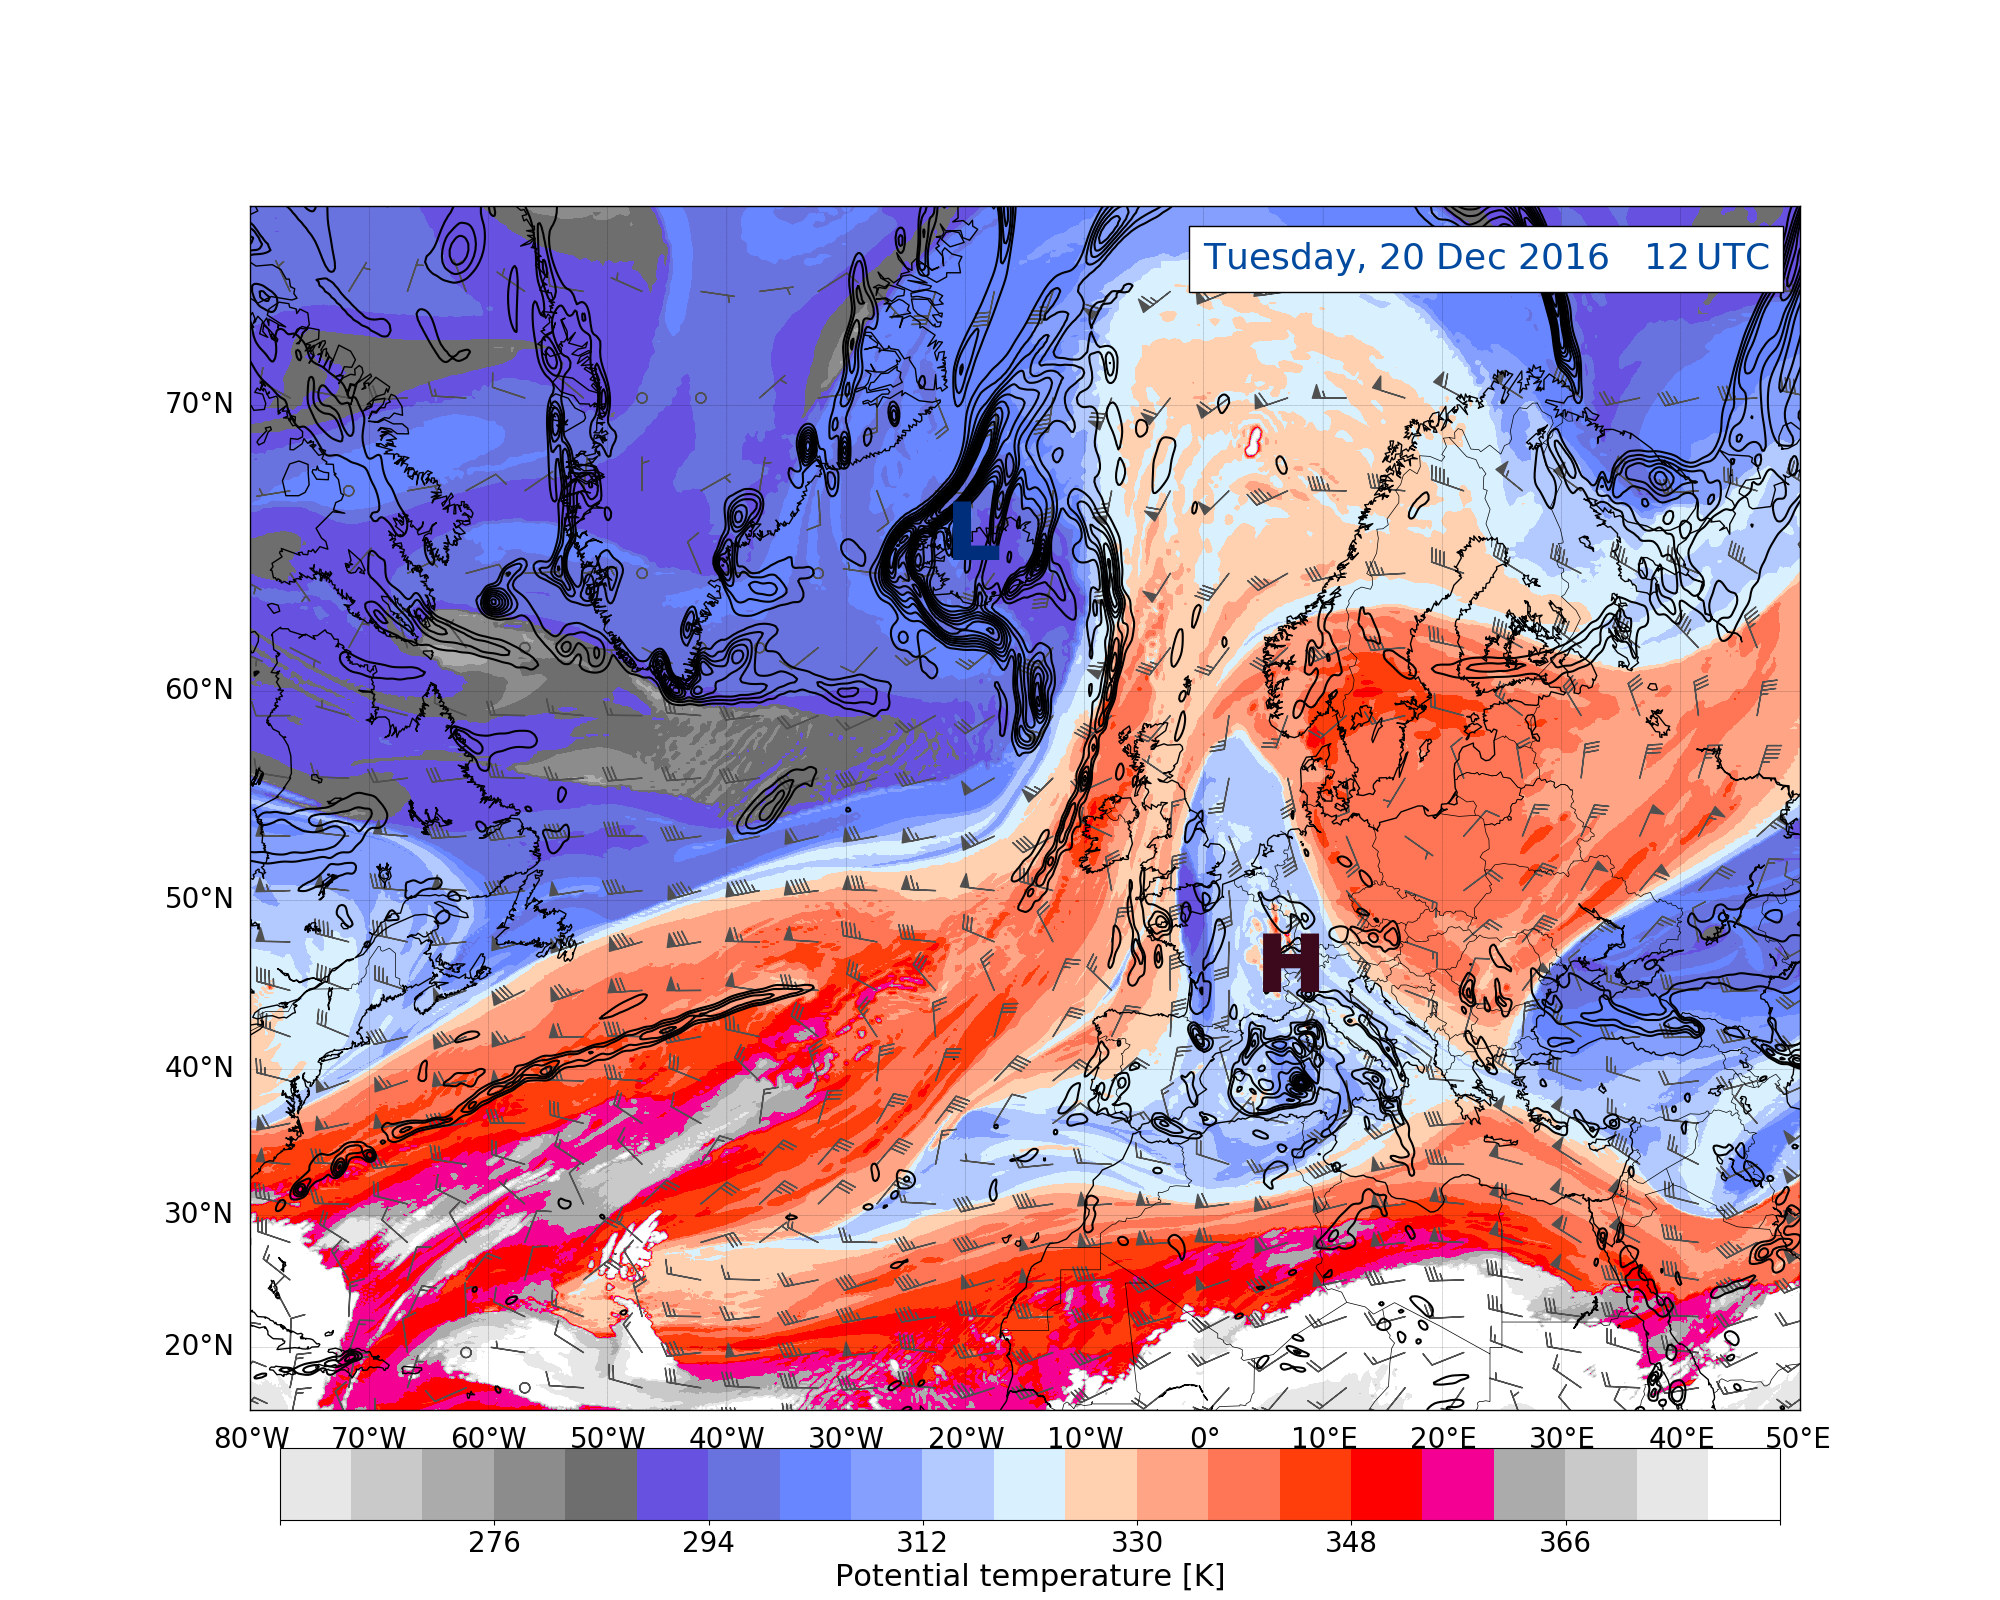
\includegraphics[trim={4.2cm 3.9cm 4.3cm 5.1cm},clip,
        width=\textwidth]{./fig_DynTropo/20161220_12}
        \caption{} \label{fig:DT20}
    \end{subfigure}
%%%%%% 21/12
    \begin{subfigure}[b]{0.49\textwidth}
        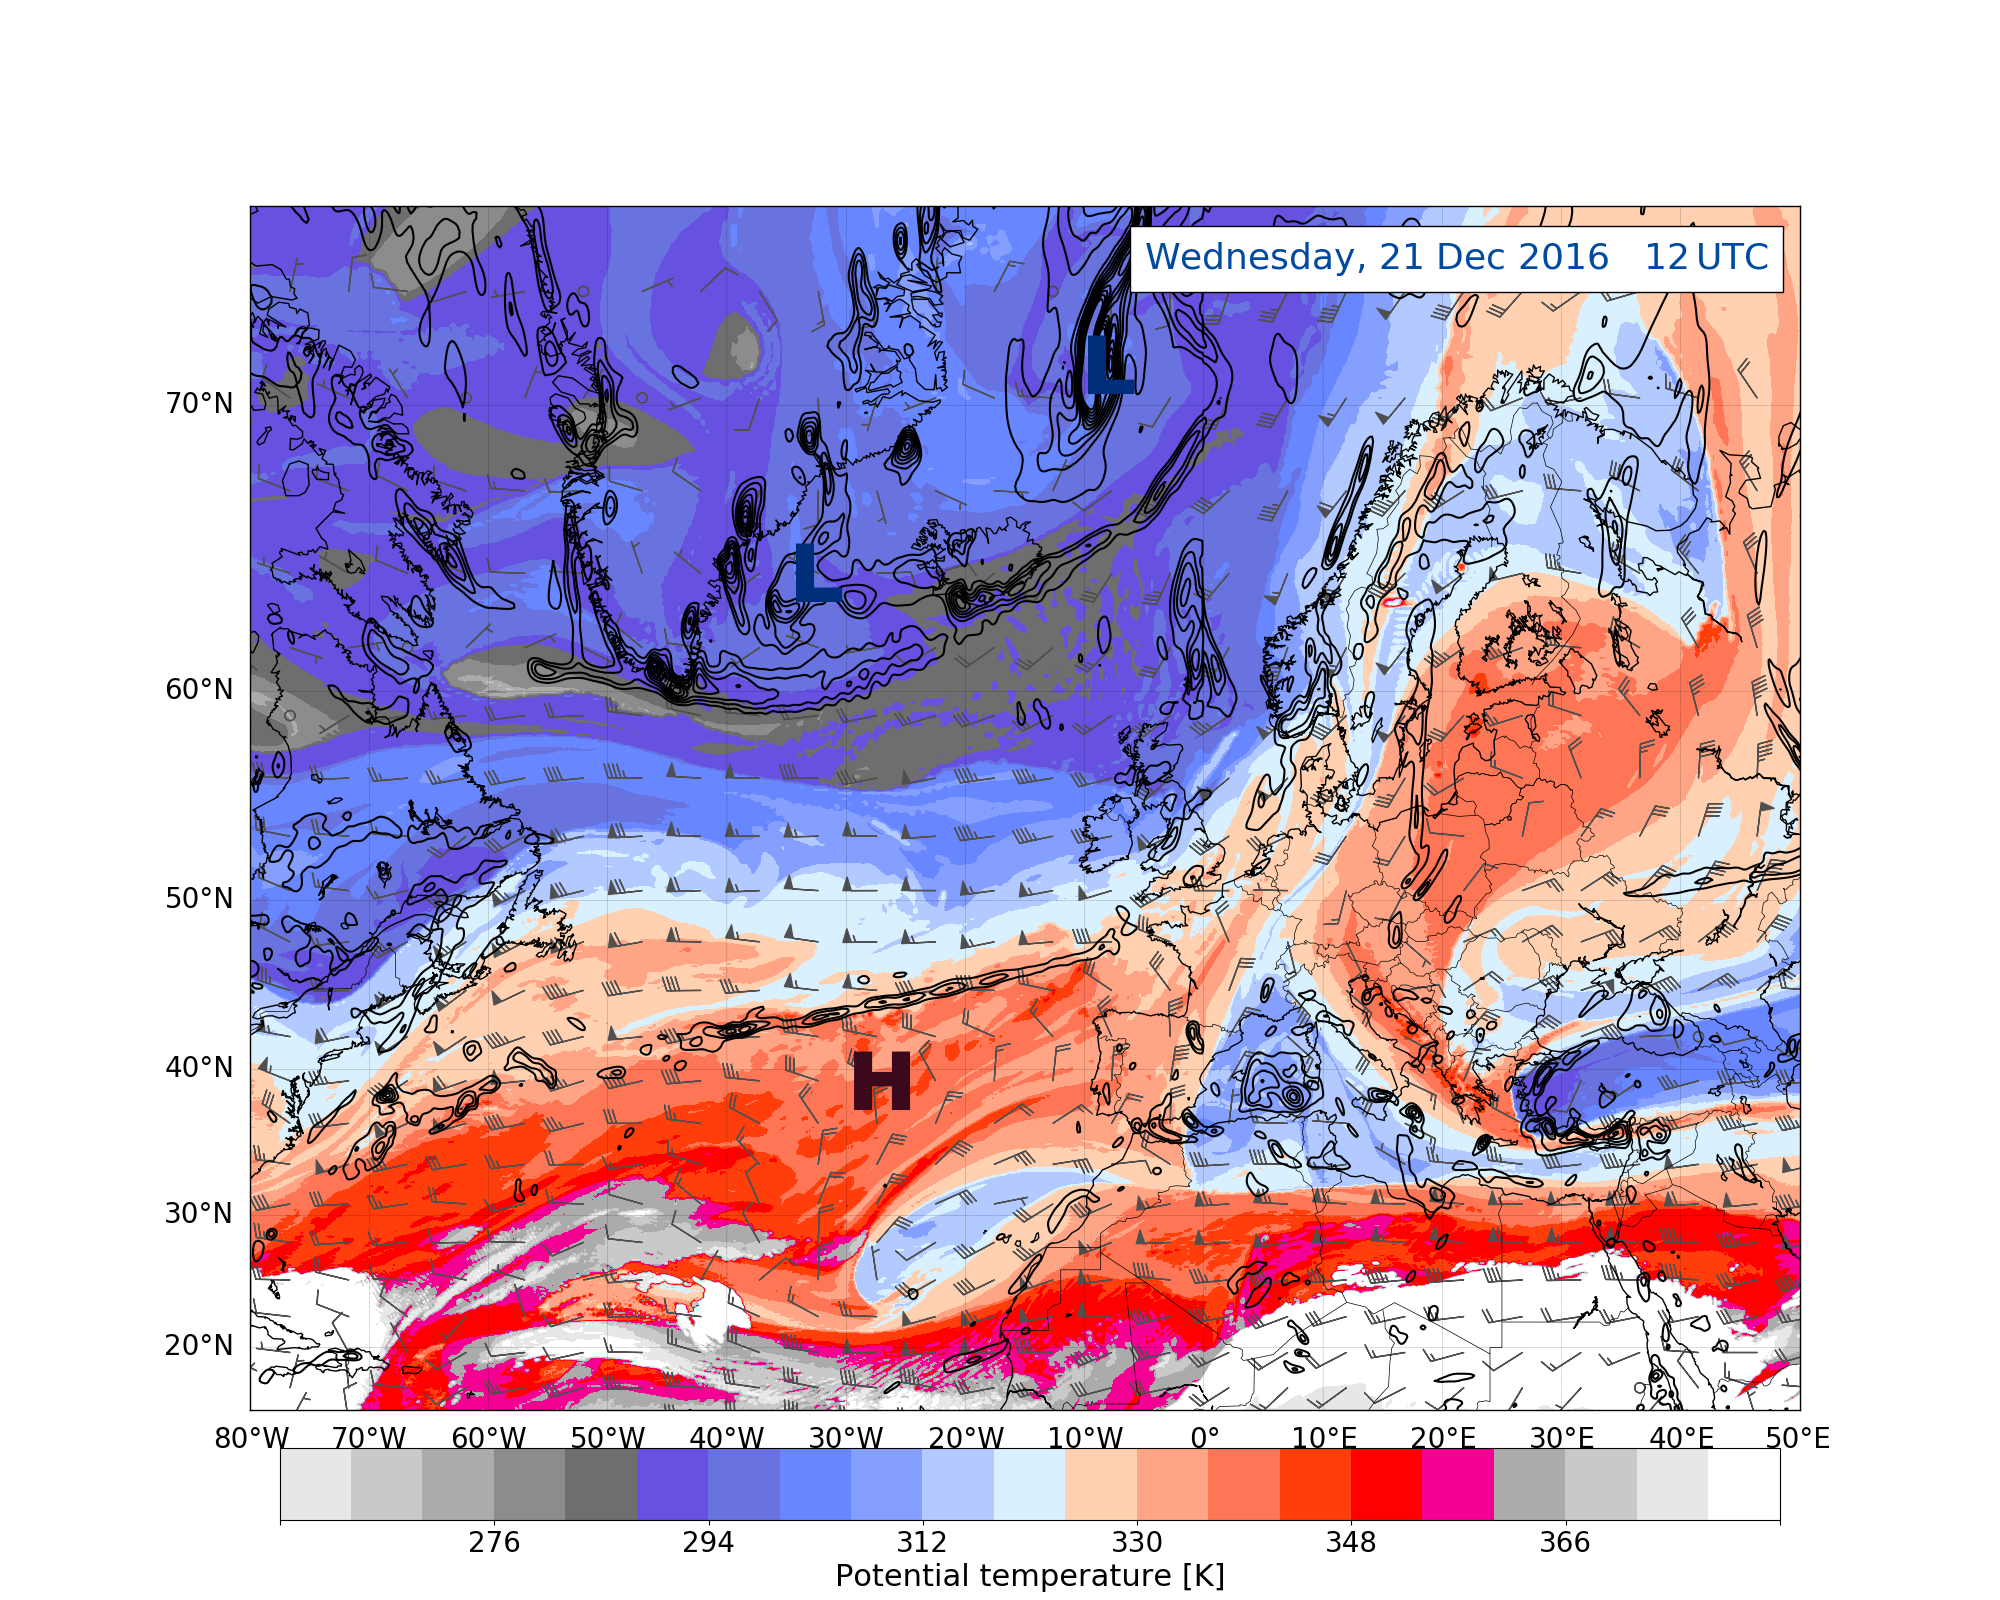
\includegraphics[trim={4.2cm 3.9cm 4.3cm 5.1cm},clip,
        width=\textwidth]{./fig_DynTropo/20161221_12}
        \caption{}\label{fig:DT21}
    \end{subfigure}

%%%%%% 22/12
\begin{subfigure}[b]{0.49\textwidth}
	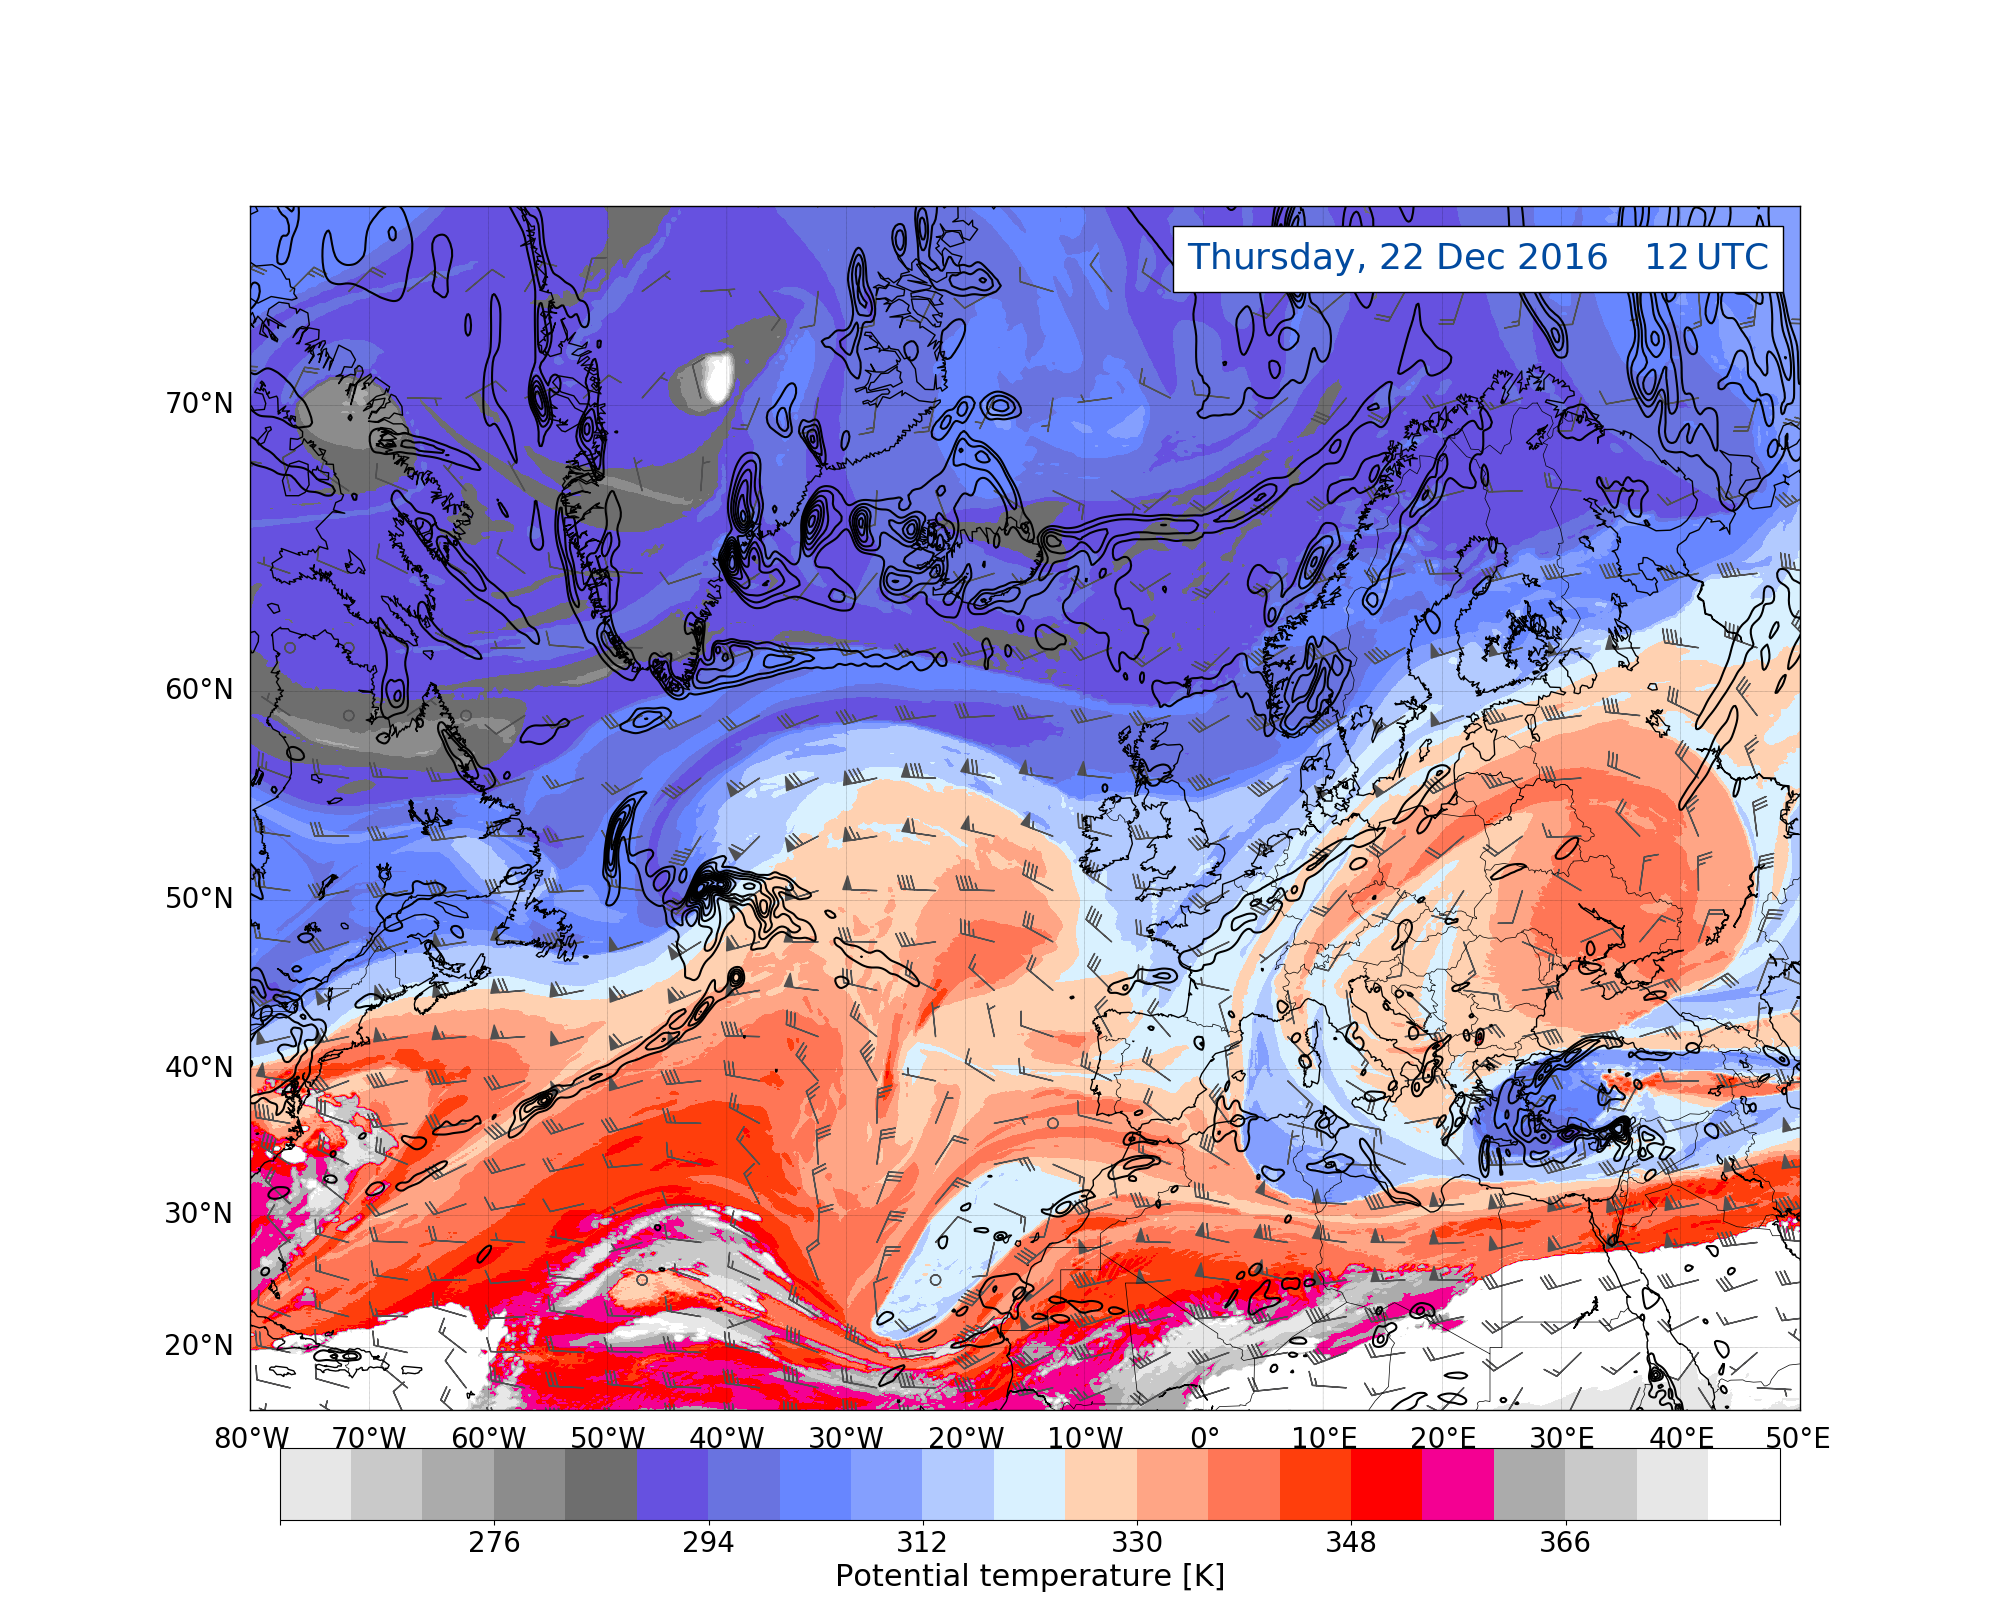
\includegraphics[trim={4.2cm 3.9cm 4.3cm 5.1cm},clip,
	width=\textwidth]{./fig_DynTropo/20161222_12}
	\caption{}\label{fig:DT22}
\end{subfigure}
%%%%%% 23/12
\begin{subfigure}[b]{0.49\textwidth}
	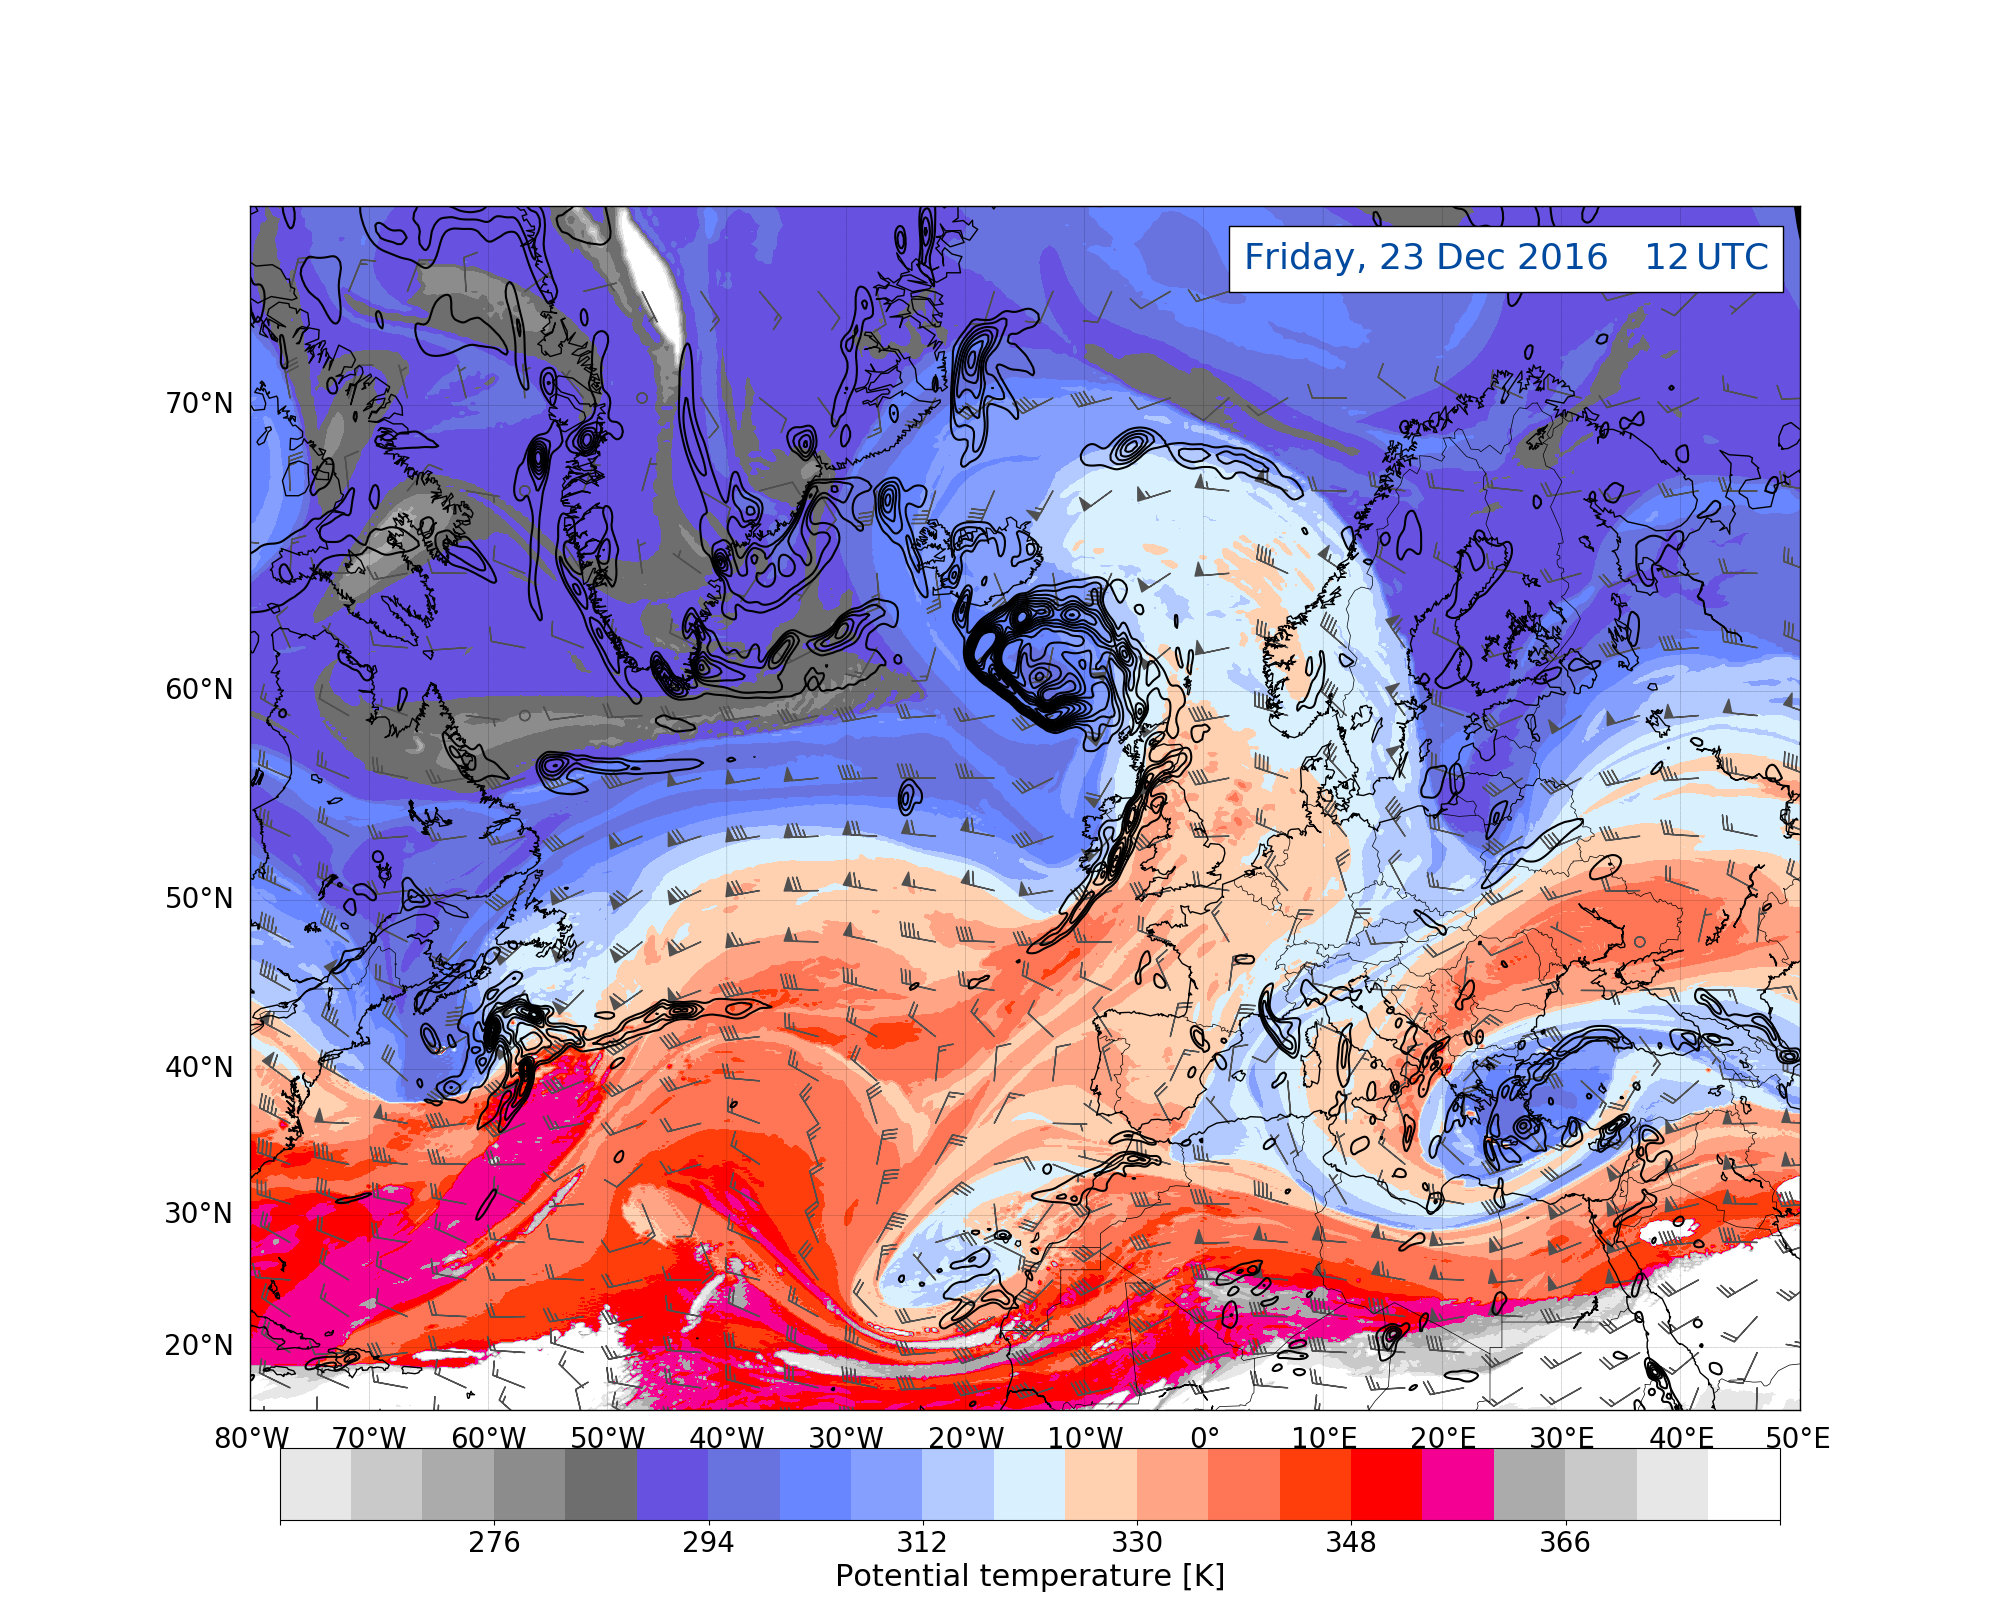
\includegraphics[trim={4.2cm 3.9cm 4.3cm 5.1cm},clip,
	width=\textwidth]{./fig_DynTropo/20161223_12}
	\caption{}\label{fig:DT23}
\end{subfigure}

%%%%%% label
    \begin{subfigure}[b]{\textwidth}
        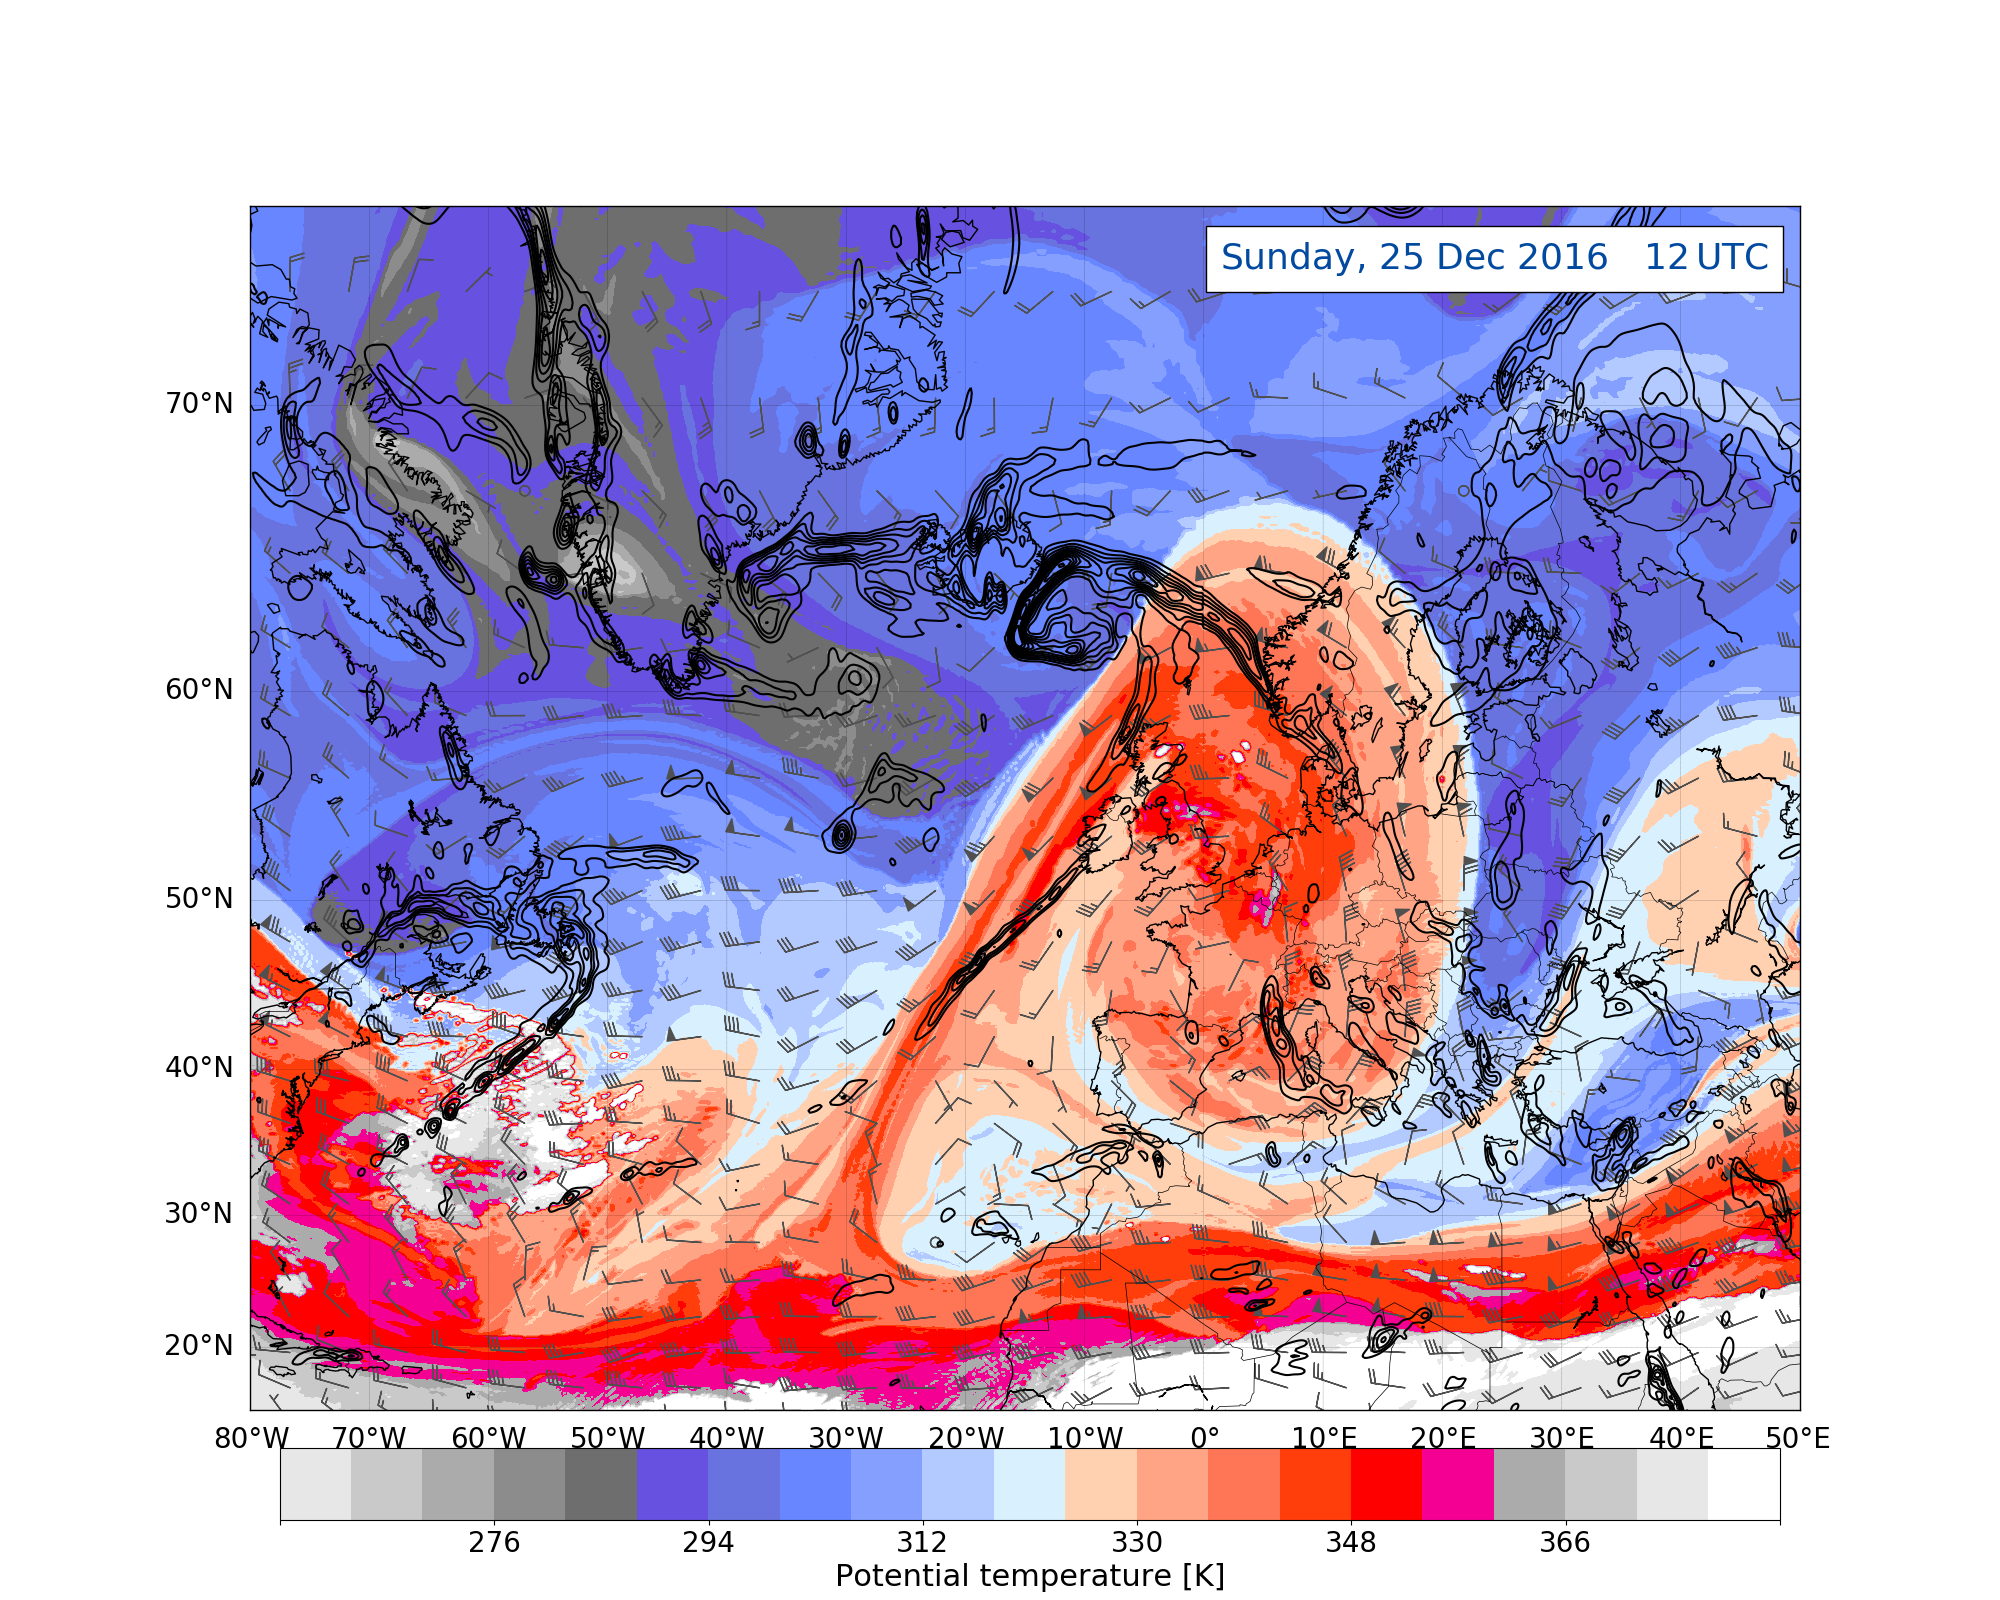
\includegraphics[trim={4.2cm 0cm 4.3cm 36.8cm},clip,
        width=\textwidth]{./fig_DynTropo/20161225_12}
    \end{subfigure}
\end{figure}
%
\begin{figure}\ContinuedFloat
	\centering
%%%%%% 24/12
    \begin{subfigure}[b]{0.49\textwidth}
        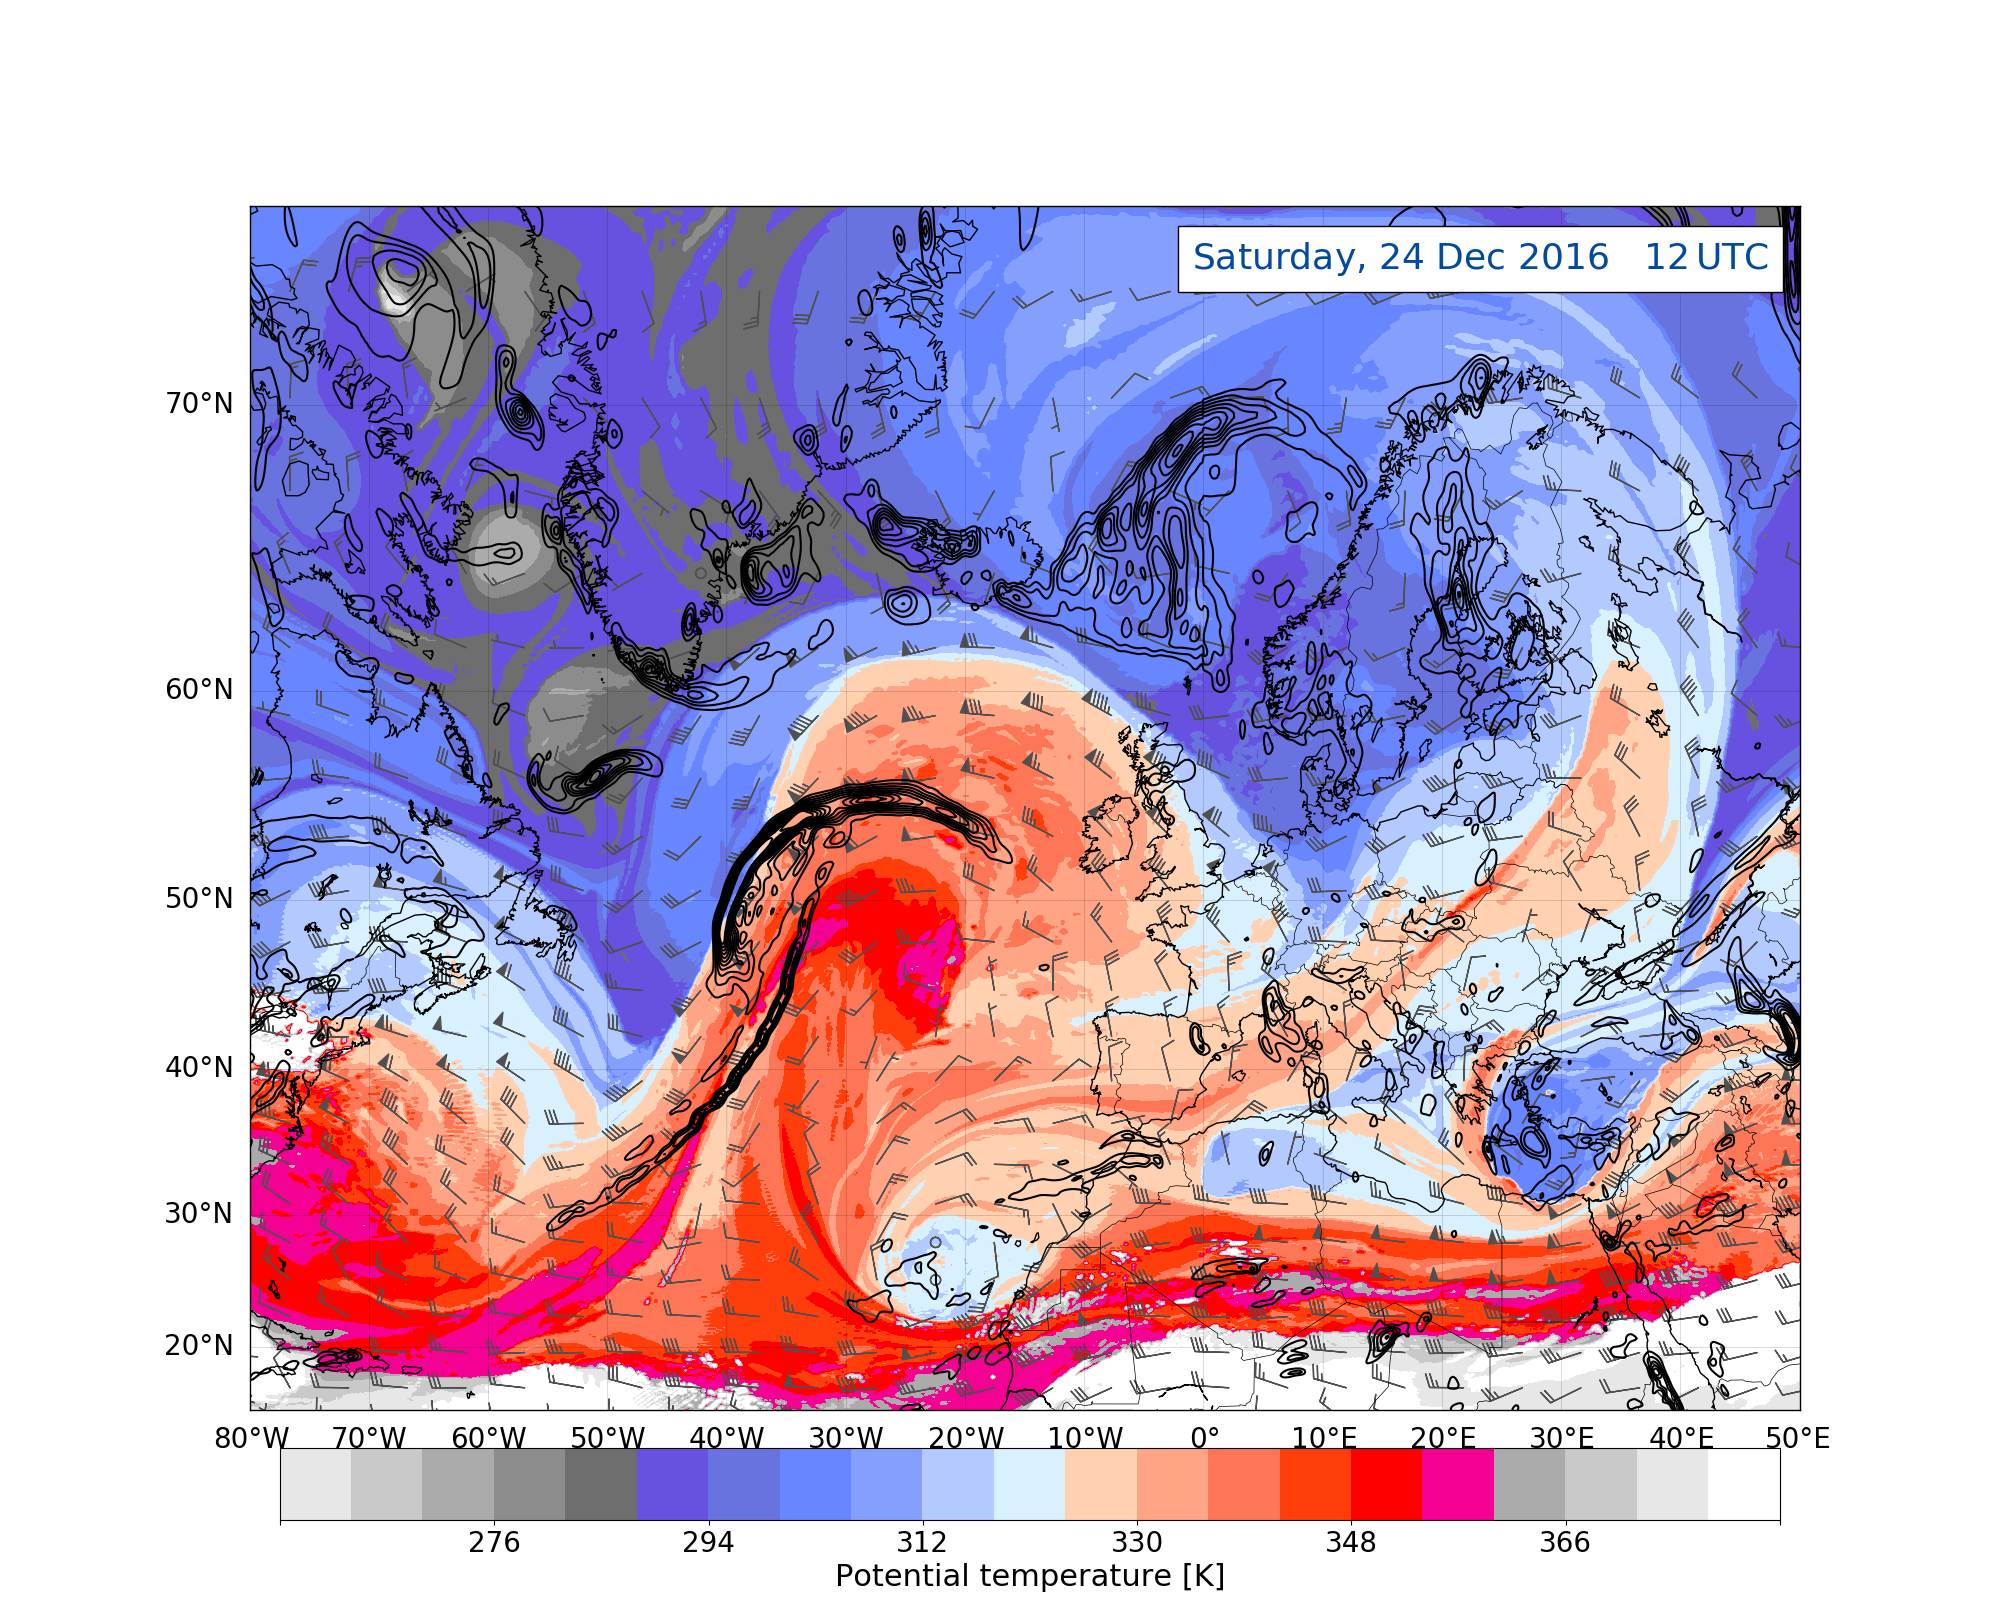
\includegraphics[trim={4.2cm 3.9cm 4.3cm 5.1cm},clip,
        width=\textwidth]{./fig_DynTropo/20161224_12}
        \caption{}\label{fig:DT24}
    \end{subfigure}
%%%%%% 25/12
    \begin{subfigure}[b]{0.49\textwidth}
        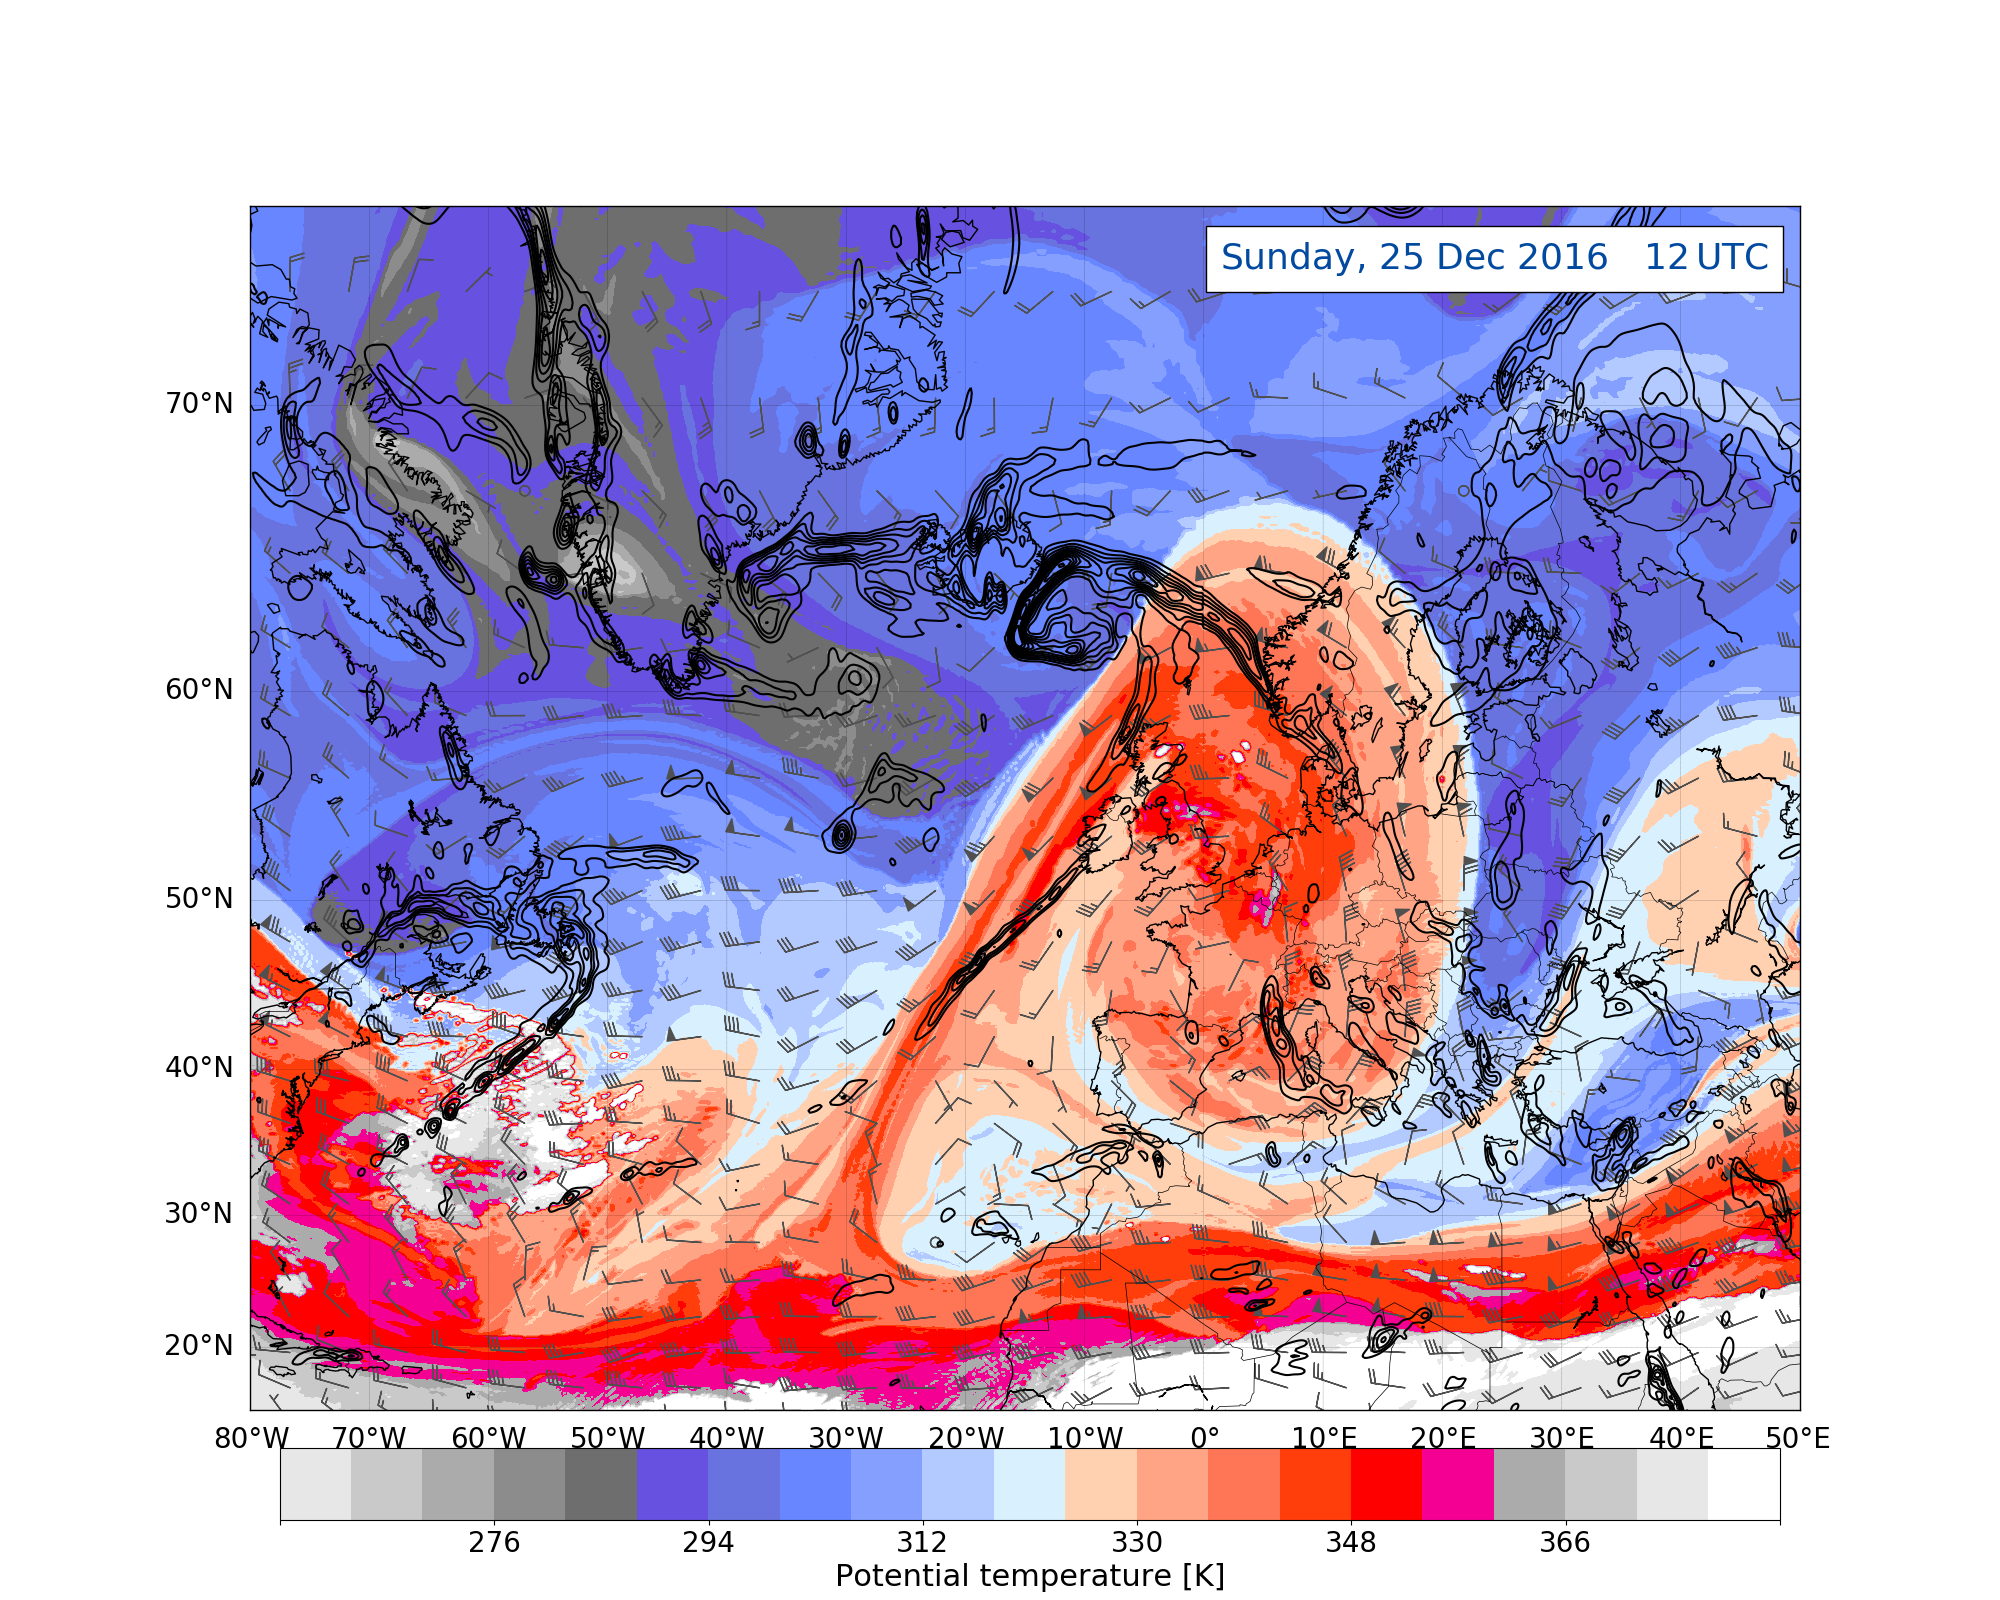
\includegraphics[trim={4.2cm 3.9cm 4.3cm 5.1cm},clip,
        width=\textwidth]{./fig_DynTropo/20161225_12}
        \caption{}\label{fig:DT25}
    \end{subfigure}    
%%%%%% 26/12
    \begin{subfigure}[b]{0.49\textwidth}
        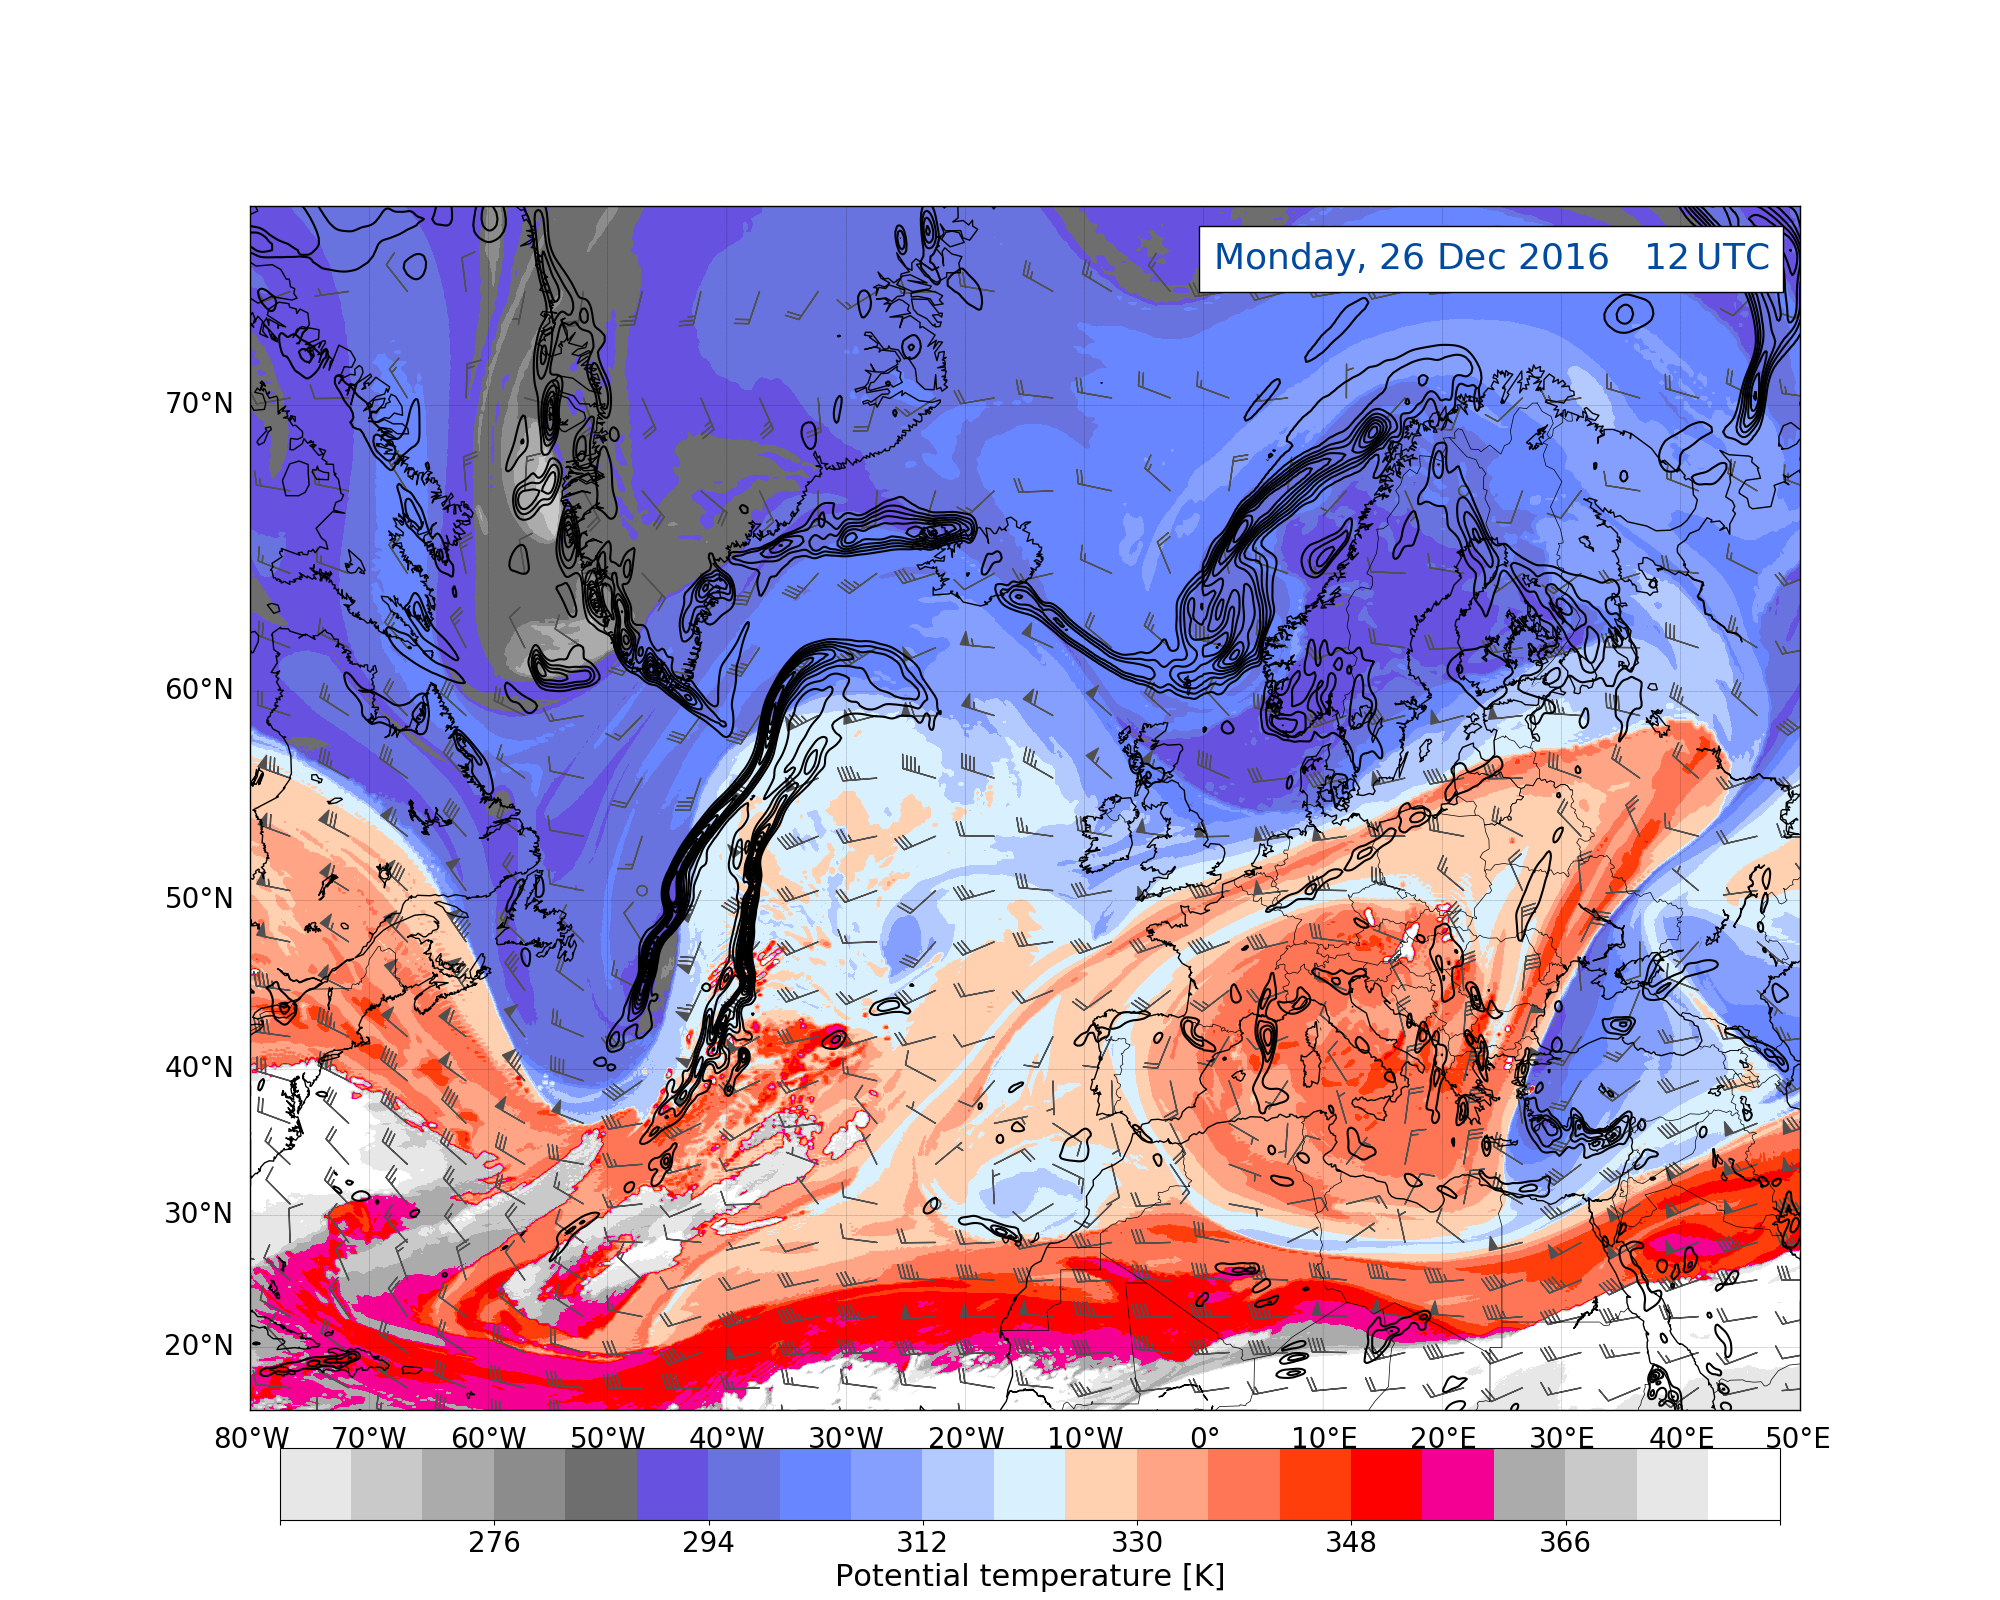
\includegraphics[trim={4.2cm 3.9cm 4.3cm 5.1cm},clip,
        width=\textwidth]{./fig_DynTropo/20161226_12}
        \caption{}\label{fig:DT26}
    \end{subfigure}
%%%%%% 27/12
    \begin{subfigure}[b]{0.49\textwidth}
        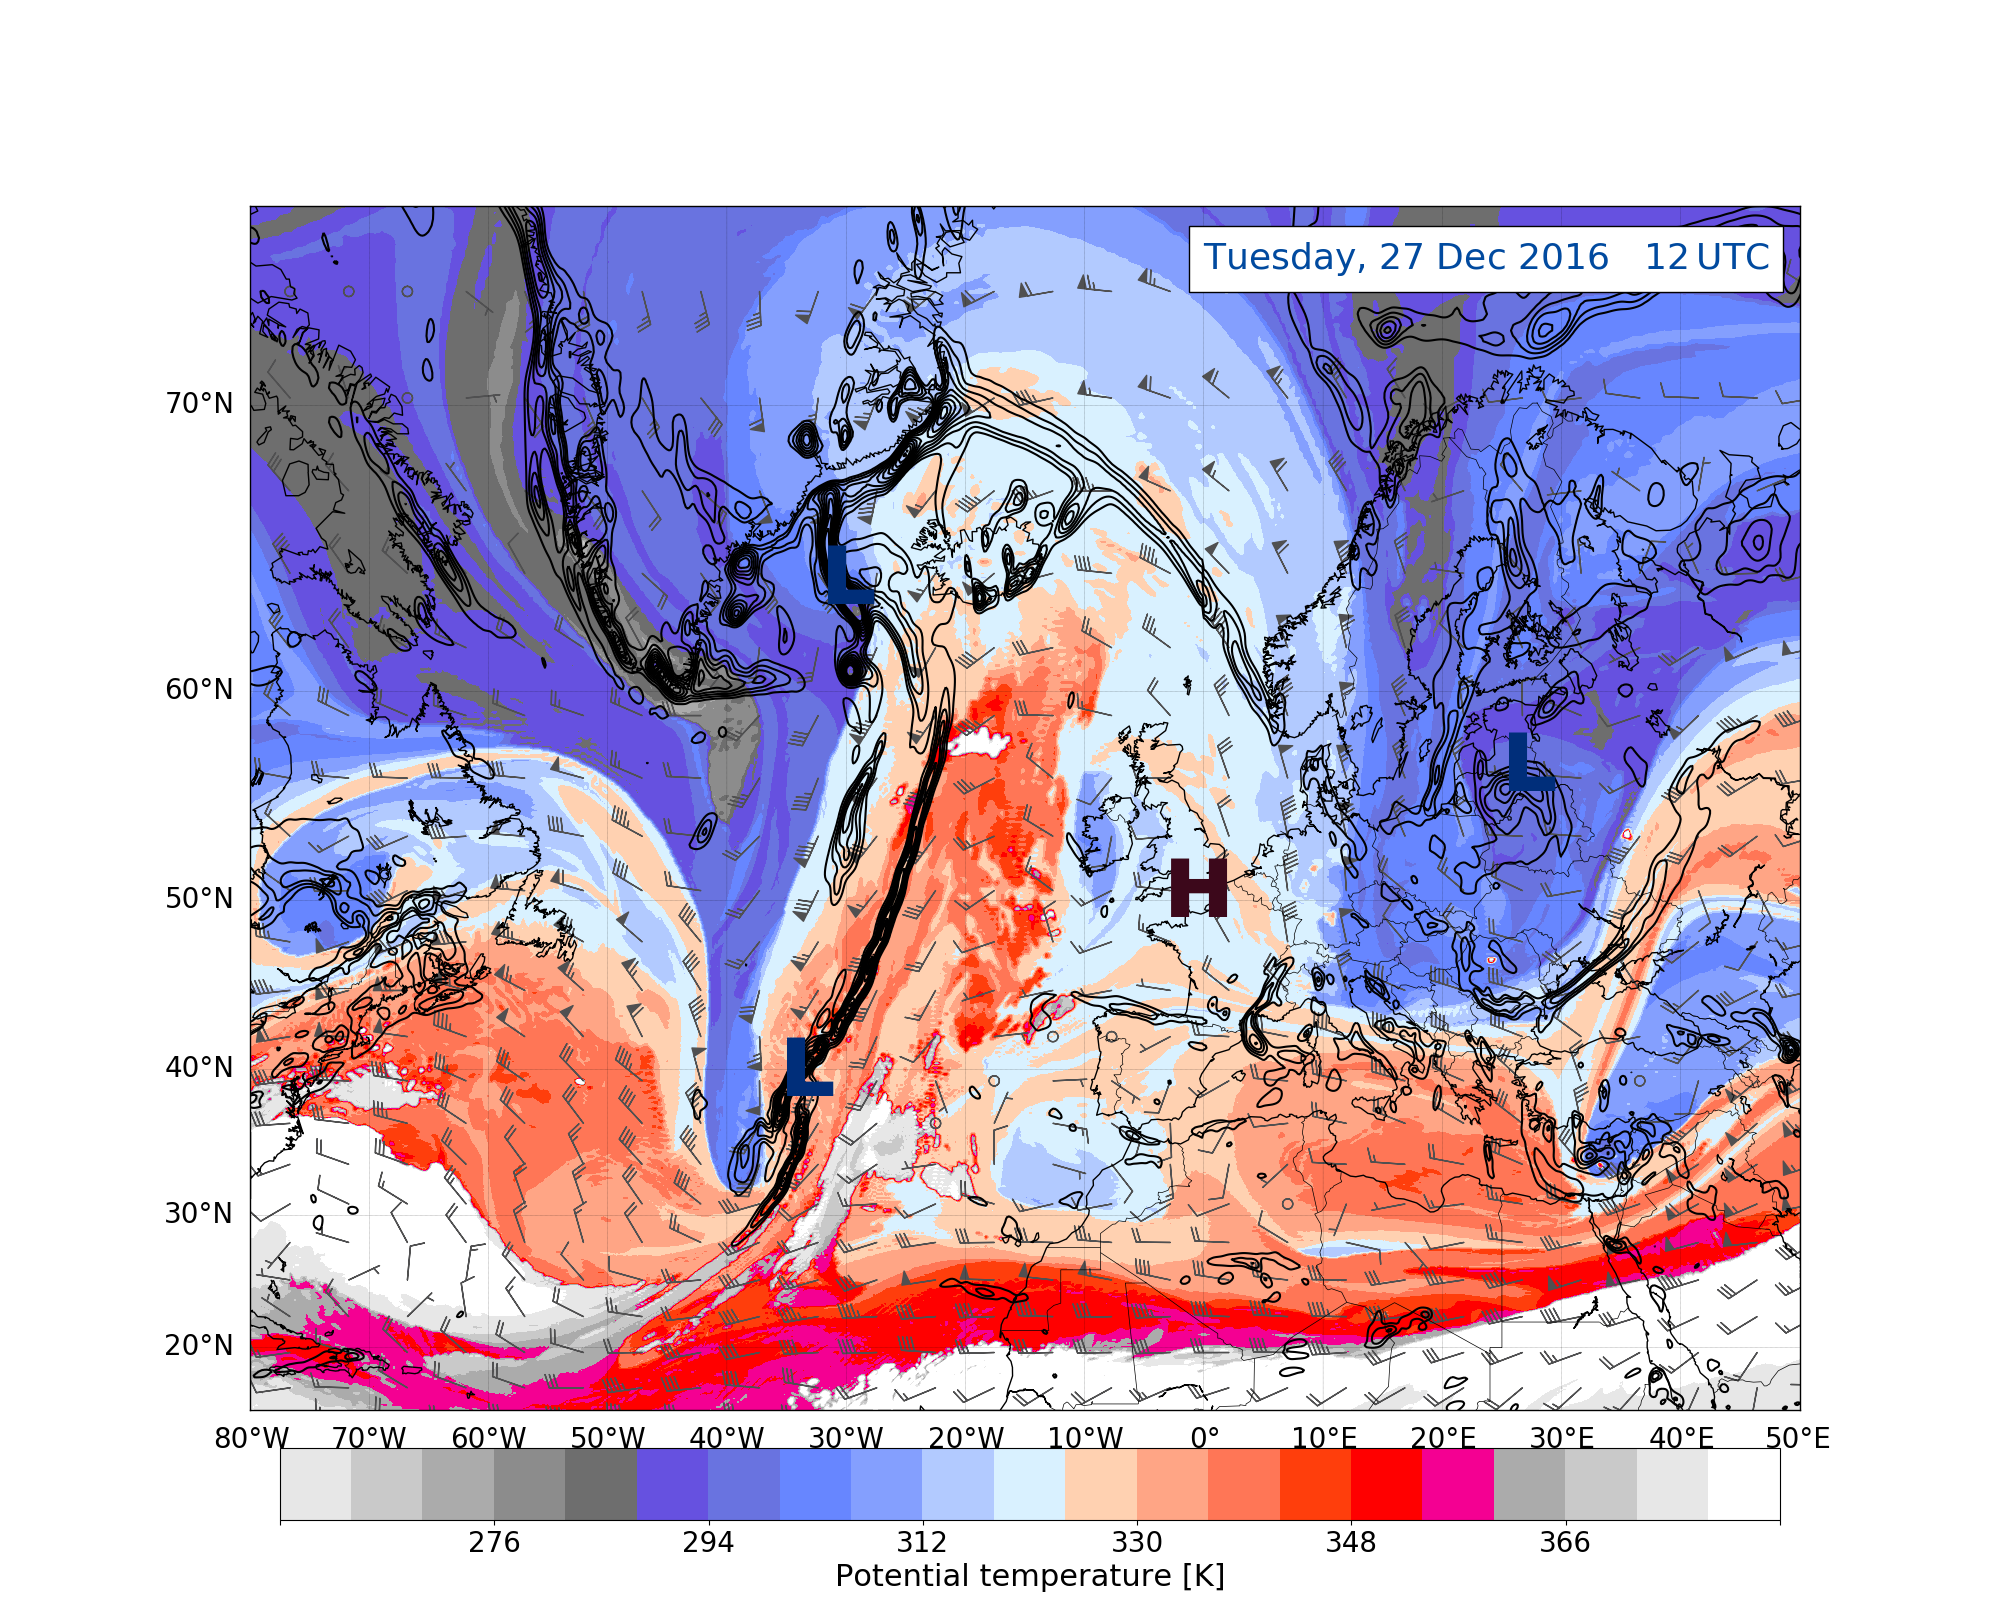
\includegraphics[trim={4.2cm 3.9cm 4.3cm 5.1cm},clip,
        width=\textwidth]{./fig_DynTropo/20161227_12}
        \caption{}\label{fig:DT27}
    \end{subfigure}   
%%%%%% label
    \begin{subfigure}[b]{\textwidth}
        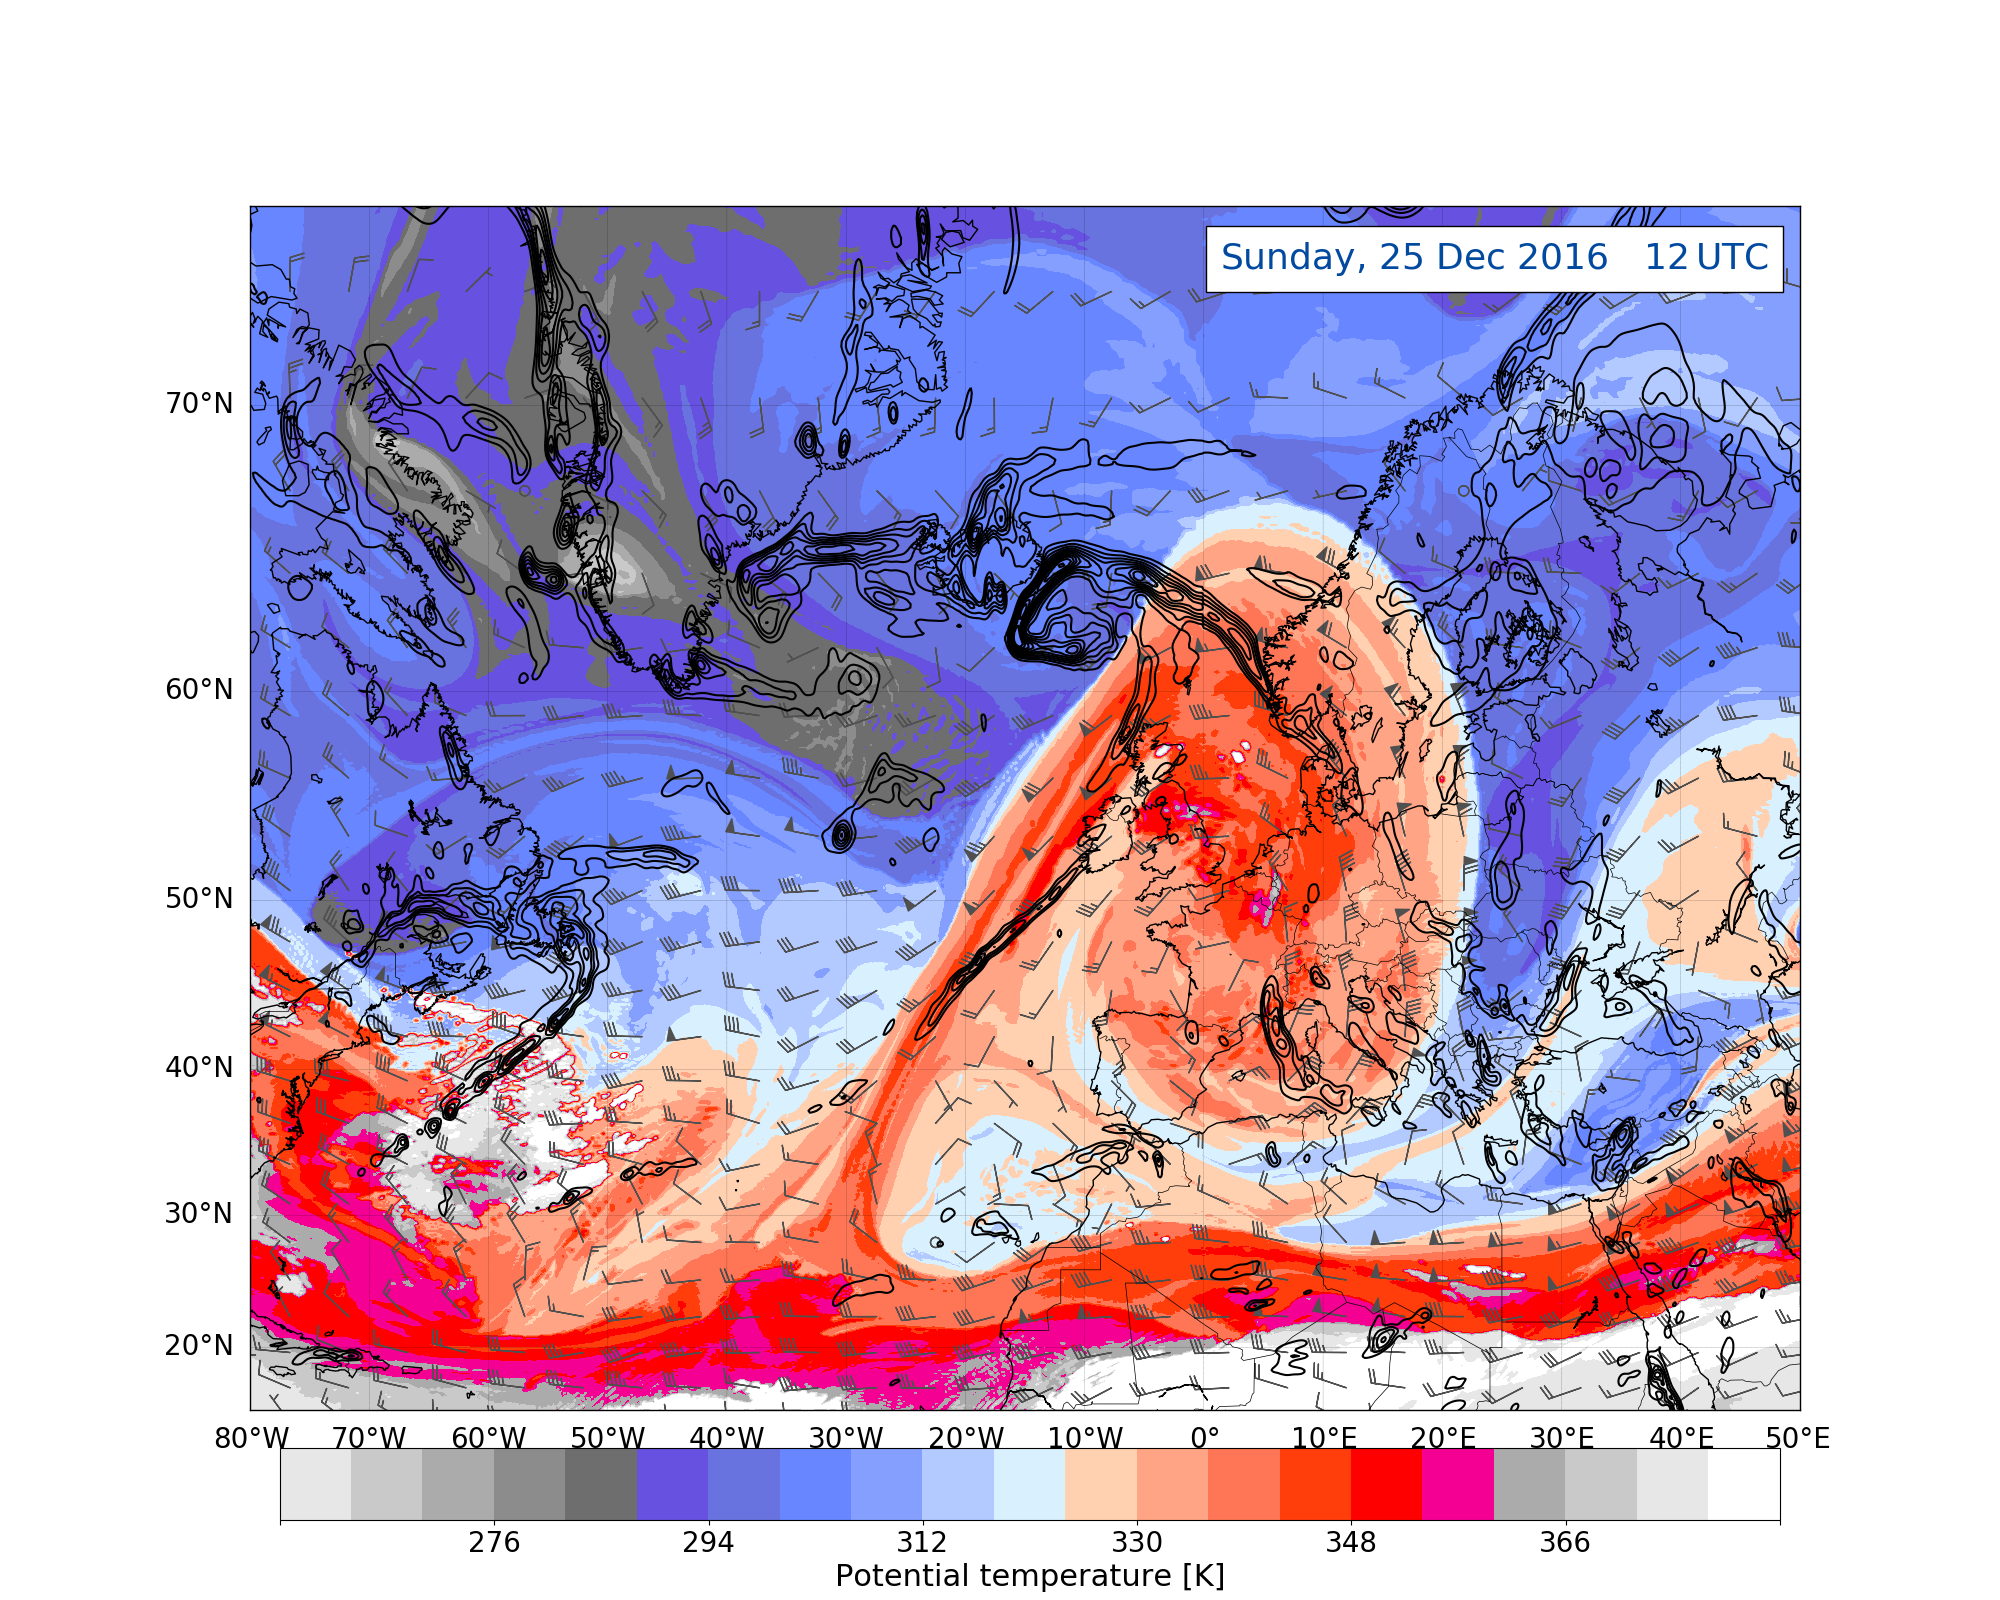
\includegraphics[trim={4.2cm 0cm 4.3cm 36.8cm},clip,
        width=\textwidth]{./fig_DynTropo/20161225_12}
    \end{subfigure}
    \caption{Dynamic tropopause analysis map, data from ECMWF at \SI{2}{PVU}. During \SIrange{20}{27}{\dec}. Potential temperature [K] at the \SI{2}{PVU} surface, shaded according to the colour bar. Total wind, barbs [\SI{}{\mPs}], and \SI{925}-\SI{850}{\hPa} layer-averaged surface relative vorticity (black contours, every \SI{.5e-4}{\per\second}).  }\label{fig:DynTropo}
\end{figure}
%%%%%%%%%%%%%%%%%%%%%%%%%%%%%%%%%%%%%%%%%%%%%%%%%%%%%%%%%%%%%%%%%%%%%%%%%%


%%%%%%%%%%%%%%%%%%%%%%%%%%%%%%%%%%%%%%%%%%%%%%%%%%%%%%%%%%%%%%%%%%%%%%%%%%
%%%%%%%%% THICKNESS MAP %%%%%%%%%%%%%%
% !TeX spellcheck = en_GB
\section{Thickness, Sea Level Pressure, Total Precipitable Water, and Wind at \SI{250}{\hPa}}
\label{sec:Geop}
%A good overview gives the sea level pressure, \SI{1000}-\SI{500}{\hPa} thickness map and winds at \SI{250}{\hPa}. \Cref{fig:GeopJet} shows, that it combines several important features of the vertical distribution within the atmosphere, for example.\\
%Black contour lines indicate sea level pressure in \SI{}{\hPa} and makes it possible to observe cyclones and anticyclones at the sea surface. 
A complementary view of the three-dimensional structure of the atmosphere is also presented:  \SI{250}{\hPa} wind speed (colour shading, \SI{}{\mPs}), mean sea level pressure (black contours, \SI{}{\hPa}), \num{1000}--\SI{500}{\hPa} thickness (dashed contours) and the total precipitable water (black-white shading, \SI{}{\mm}). See \Cref{fig:GP24_pres} for an example.
% %%% Geopot Jet maps %%%%%%%%%%%%%%%%%%%%%%%%%%%%%%%%%%%%%
% % !TeX spellcheck = en_GB

\begin{figure}[h!]
    \centering
%%%%%% 20/12
    \begin{subfigure}[b]{0.49\textwidth}
        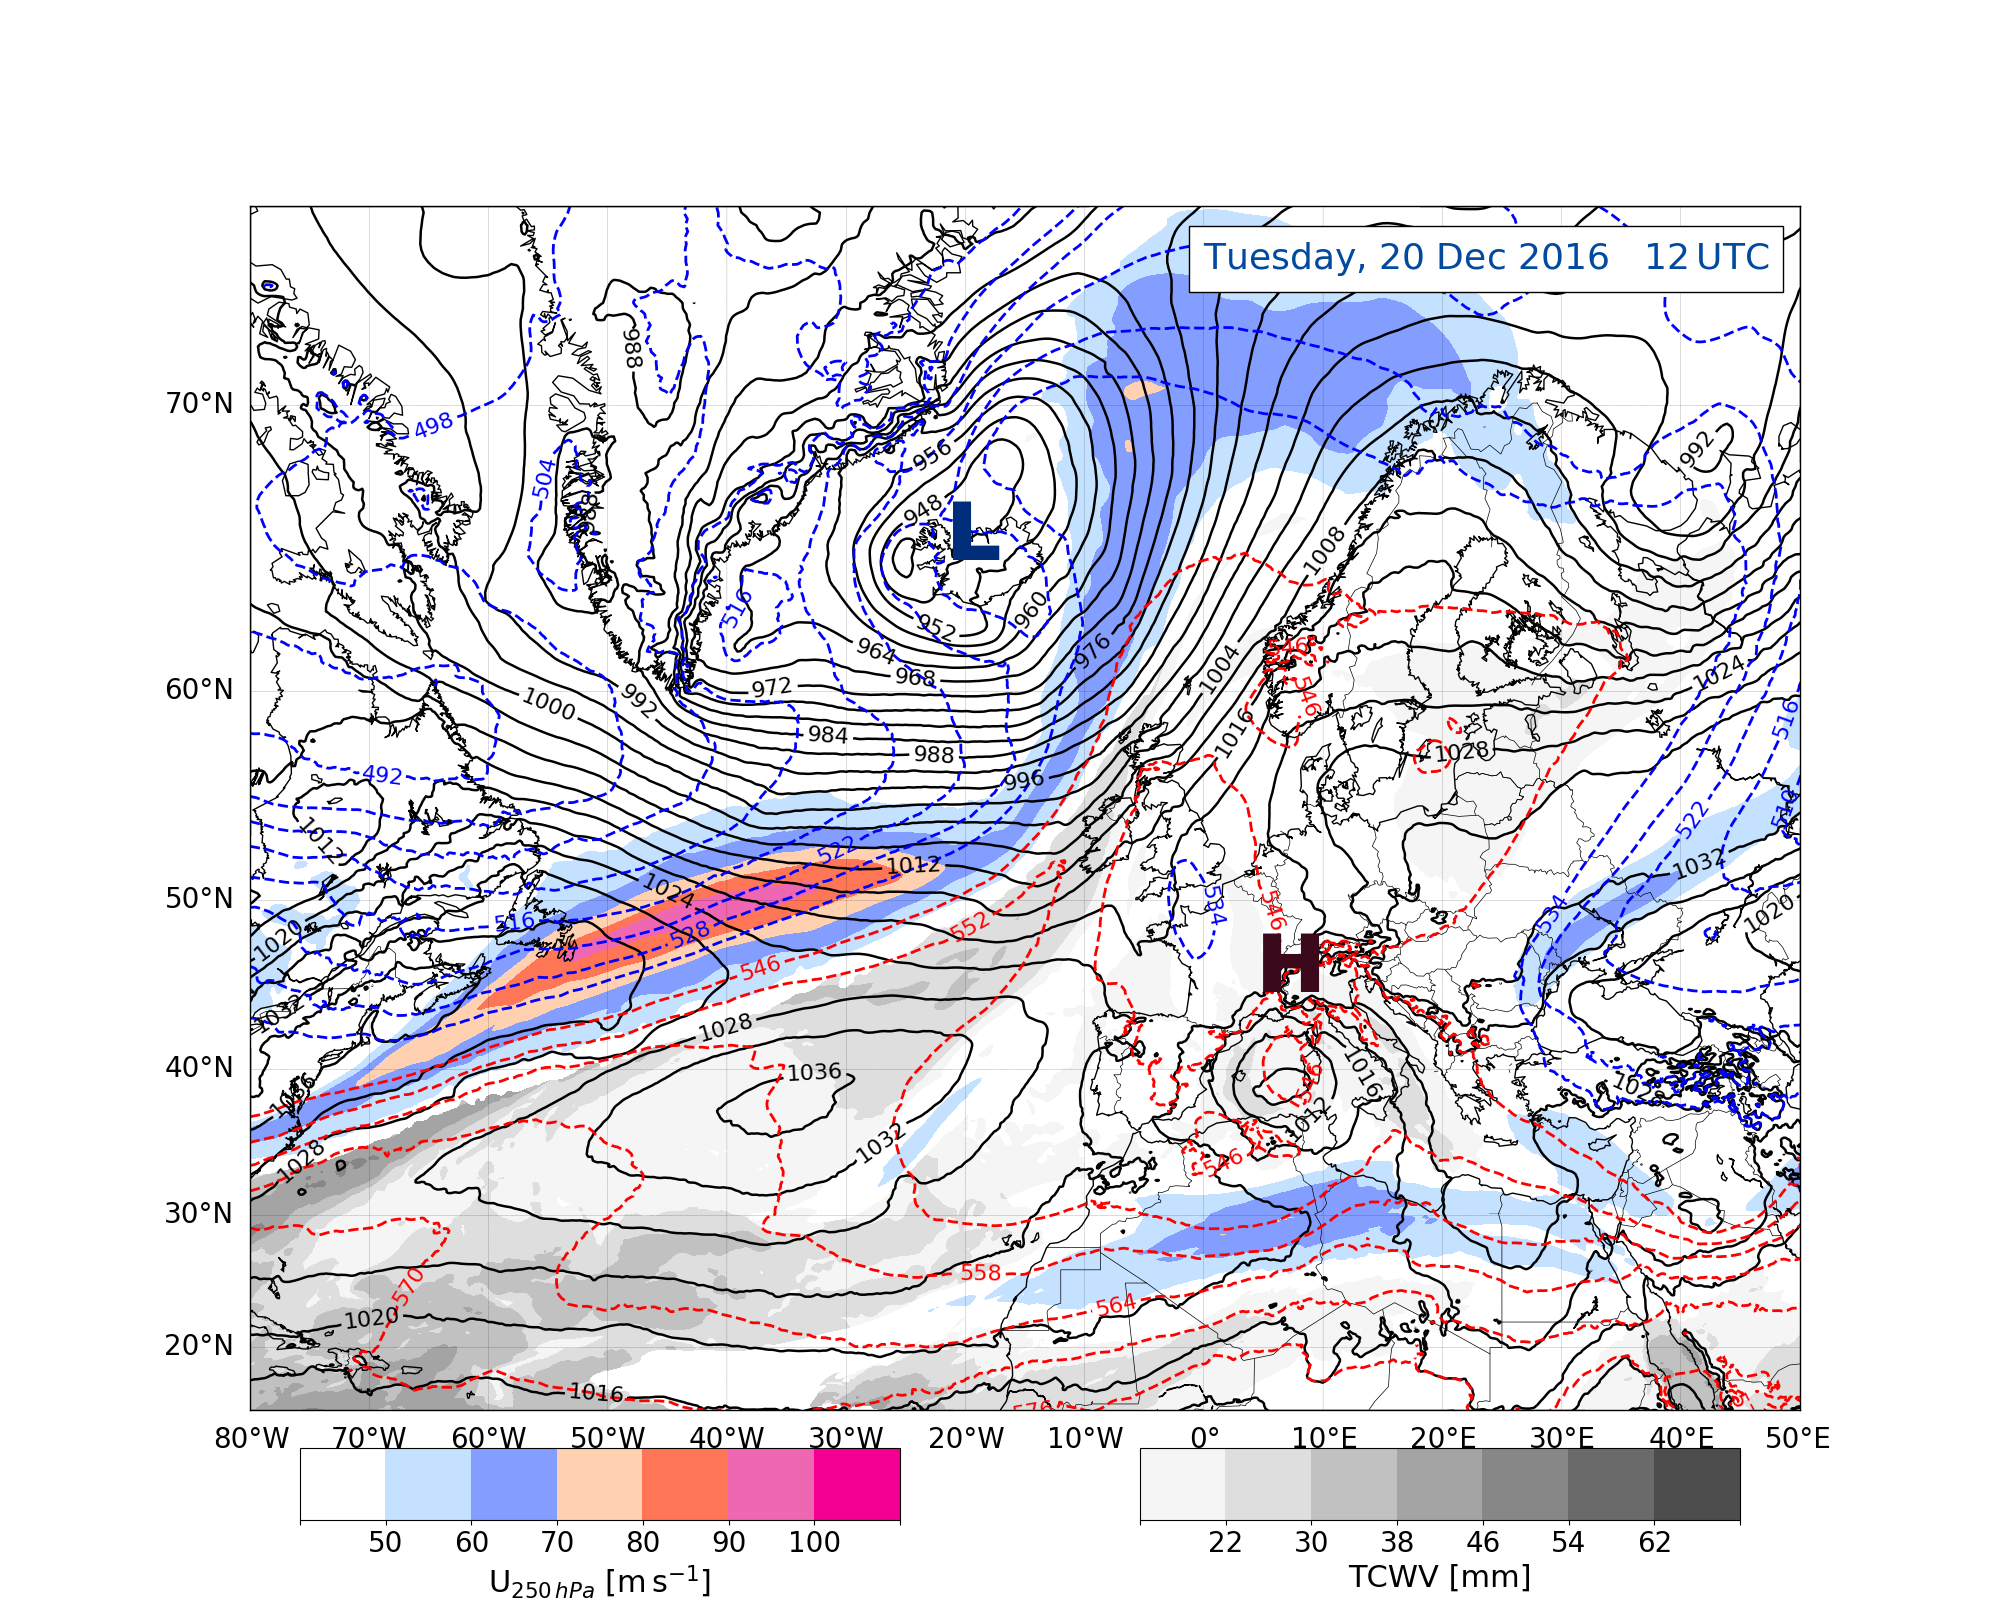
\includegraphics[trim={4.2cm 3.9cm 4.3cm 5.1cm},clip,
        width=\textwidth]{./fig_Geopot_Jet/20161220_12}
        \caption{}\label{fig:GP20}
        %\label{fig:DT2100}
    \end{subfigure}
%%%%%% 21/12
    \begin{subfigure}[b]{0.49\textwidth}
        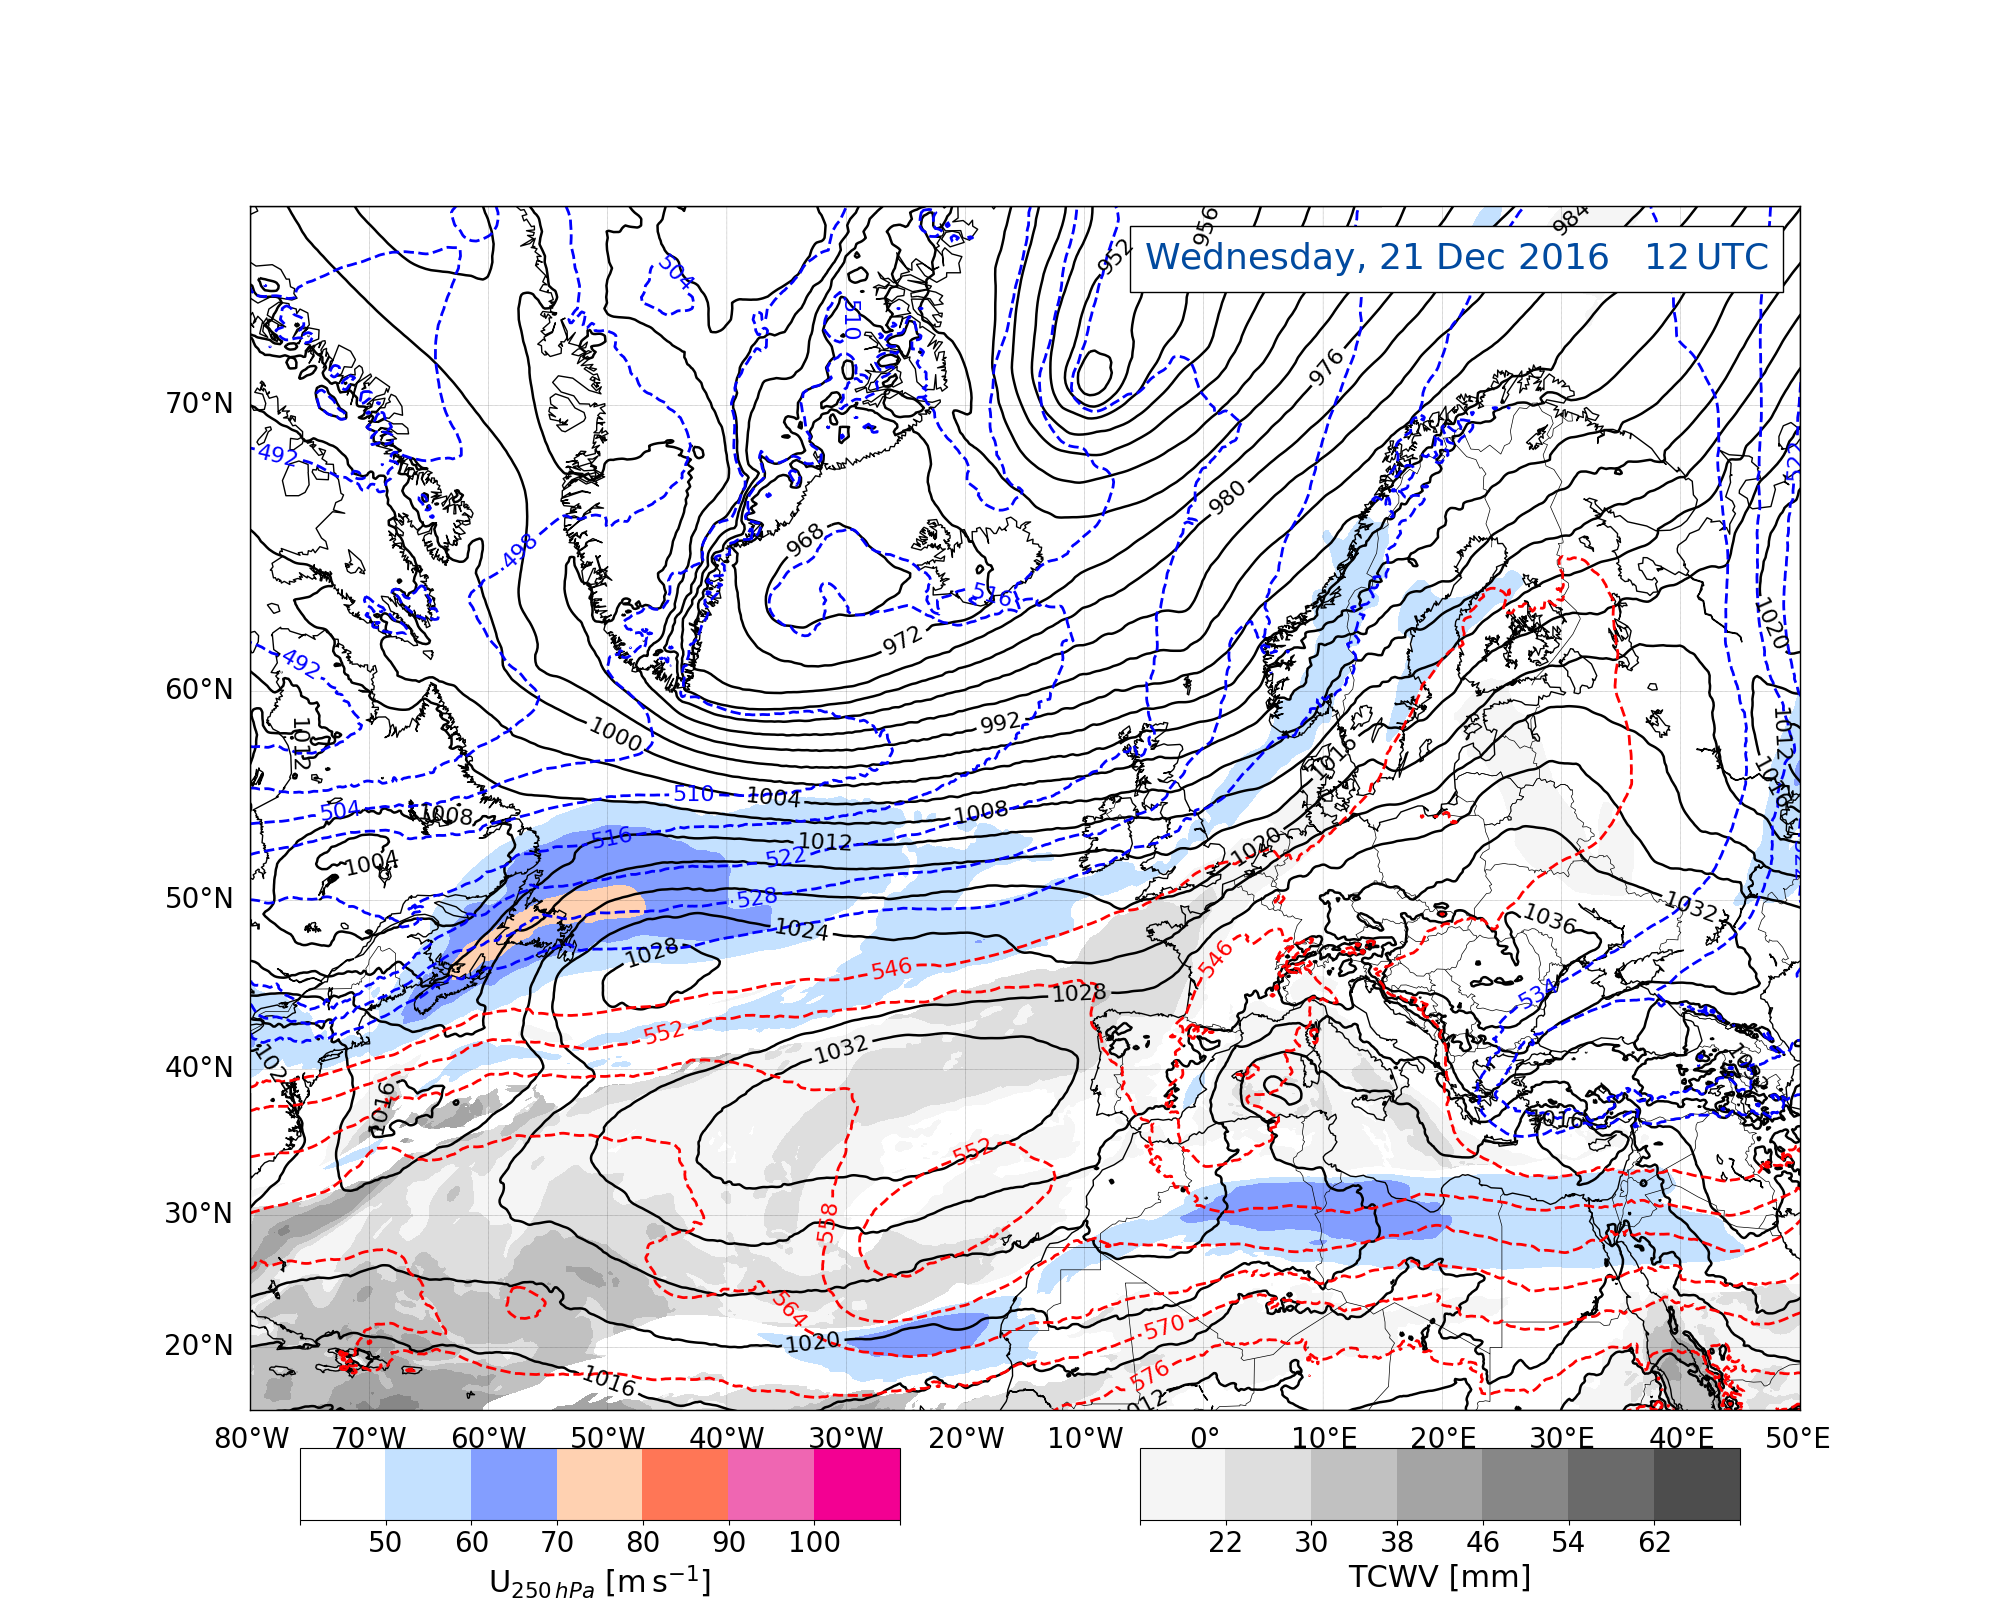
\includegraphics[trim={4.2cm 3.9cm 4.3cm 5.1cm},clip,
        width=\textwidth]{./fig_Geopot_Jet/20161221_12}
        \caption{}\label{fig:GP21}
    \end{subfigure}
%%%%%% 22/12
	\begin{subfigure}[b]{0.49\textwidth}
		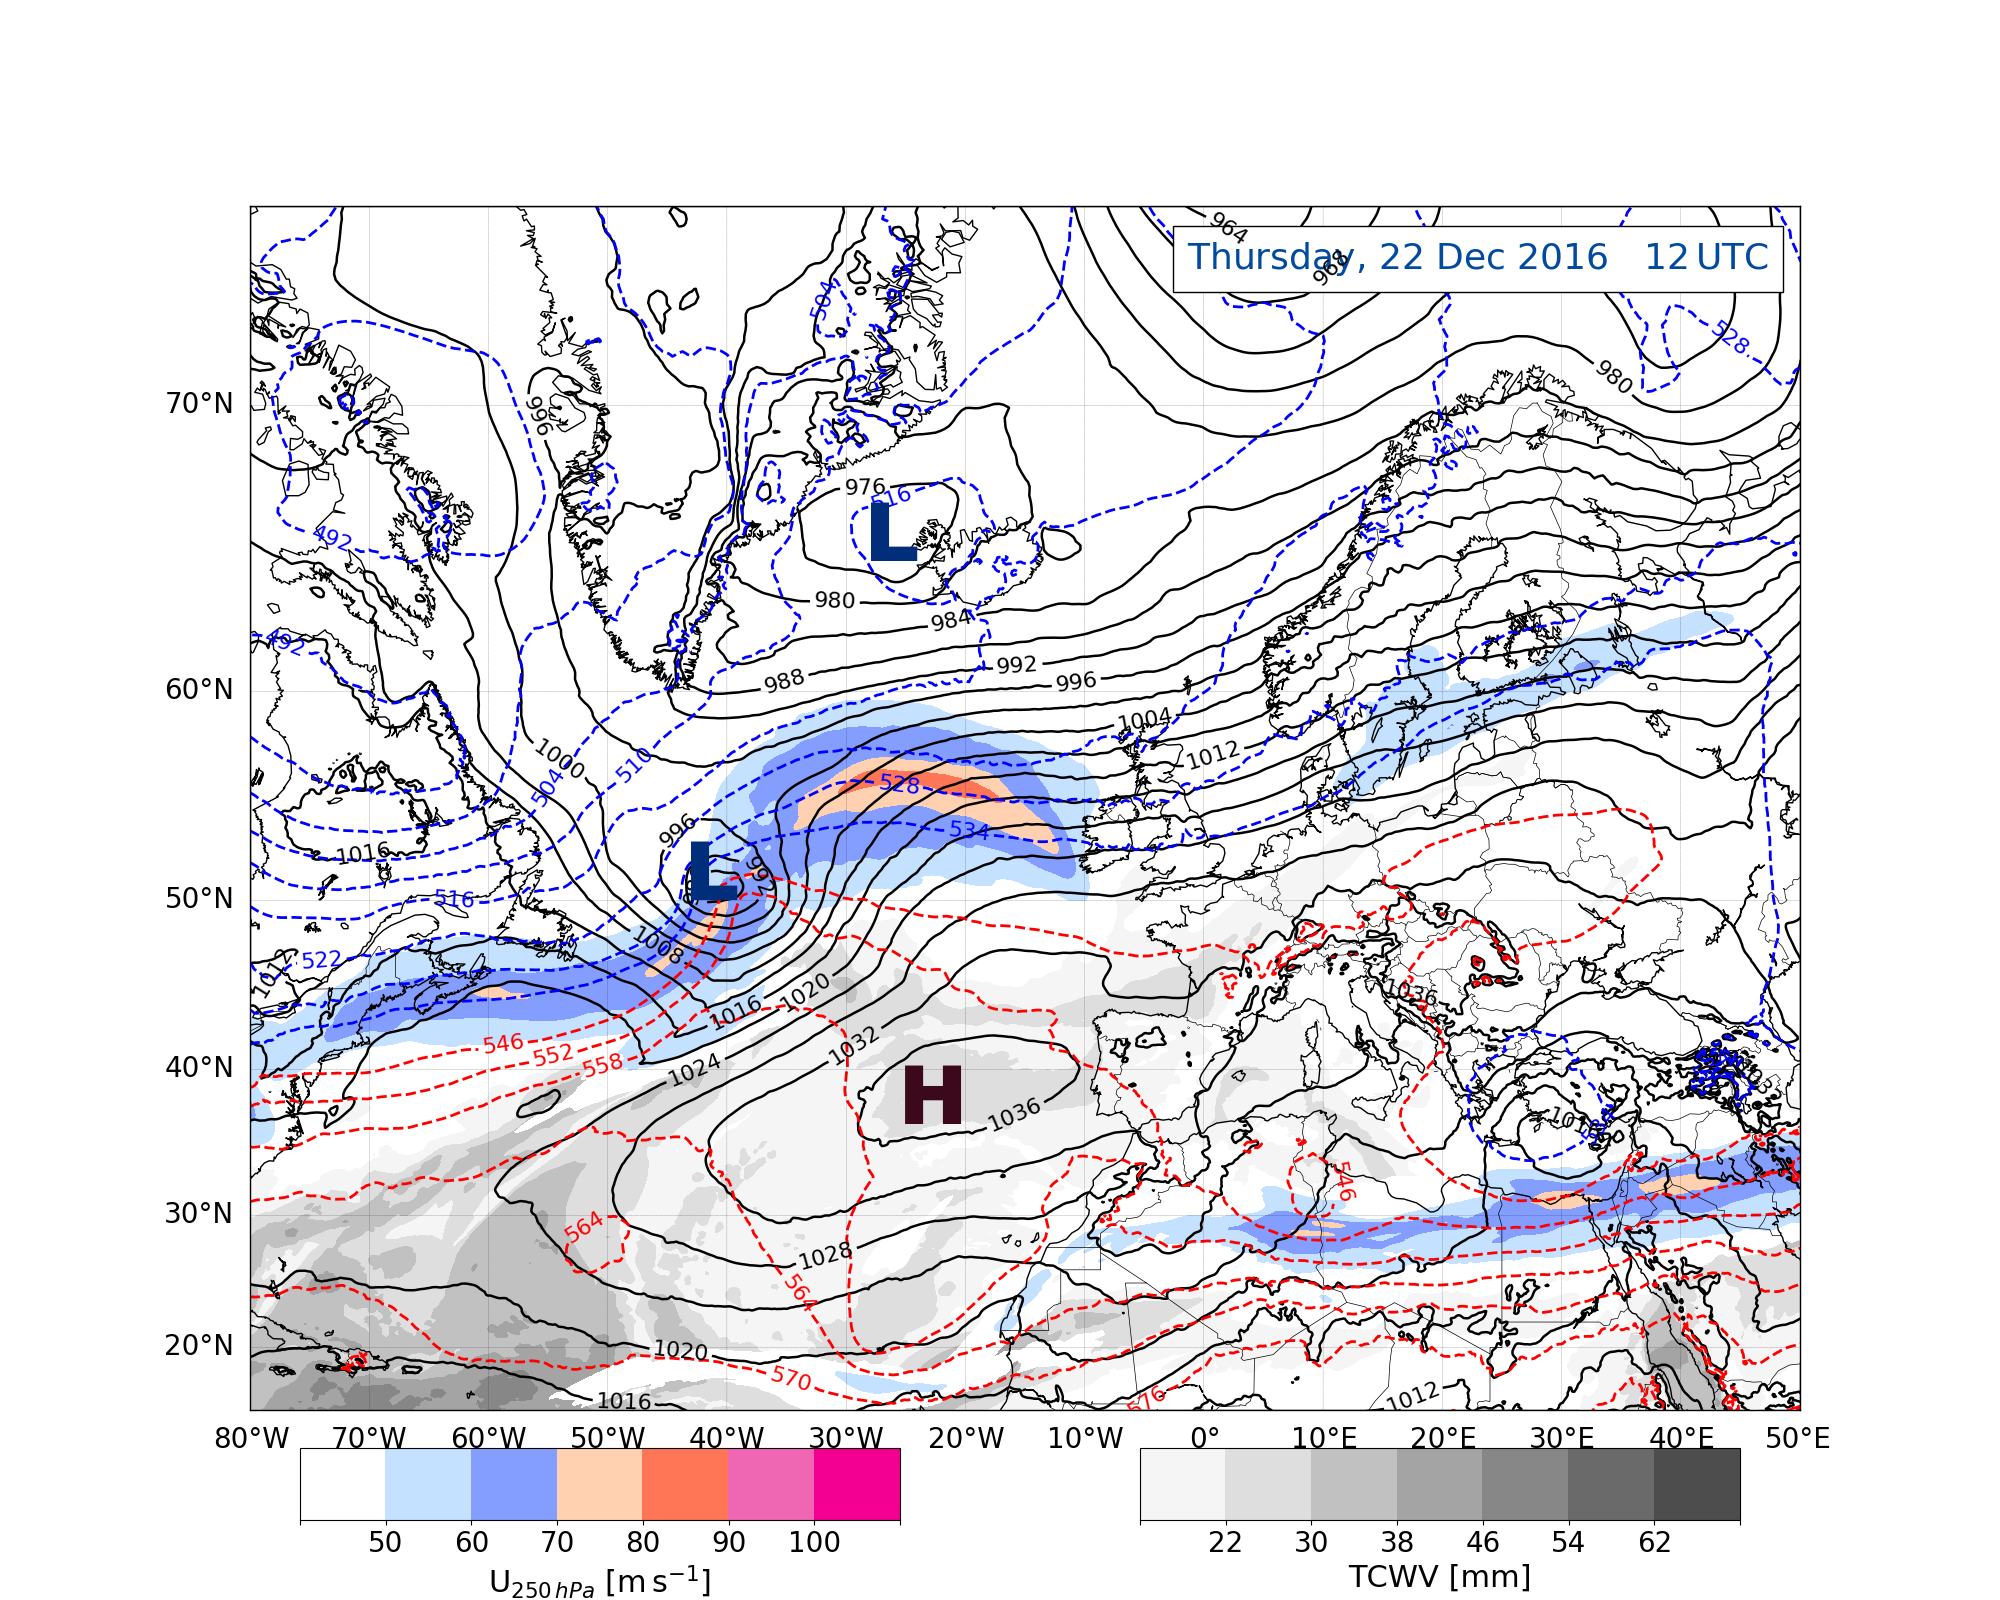
\includegraphics[trim={4.2cm 3.9cm 4.3cm 5.1cm},clip,
	width=\textwidth]{./fig_Geopot_Jet/20161222_12}
		\caption{}\label{fig:GP22}
	%\label{fig:sfc2100}
	\end{subfigure}
%%%%%% 23/12
	\begin{subfigure}[b]{0.49\textwidth}
		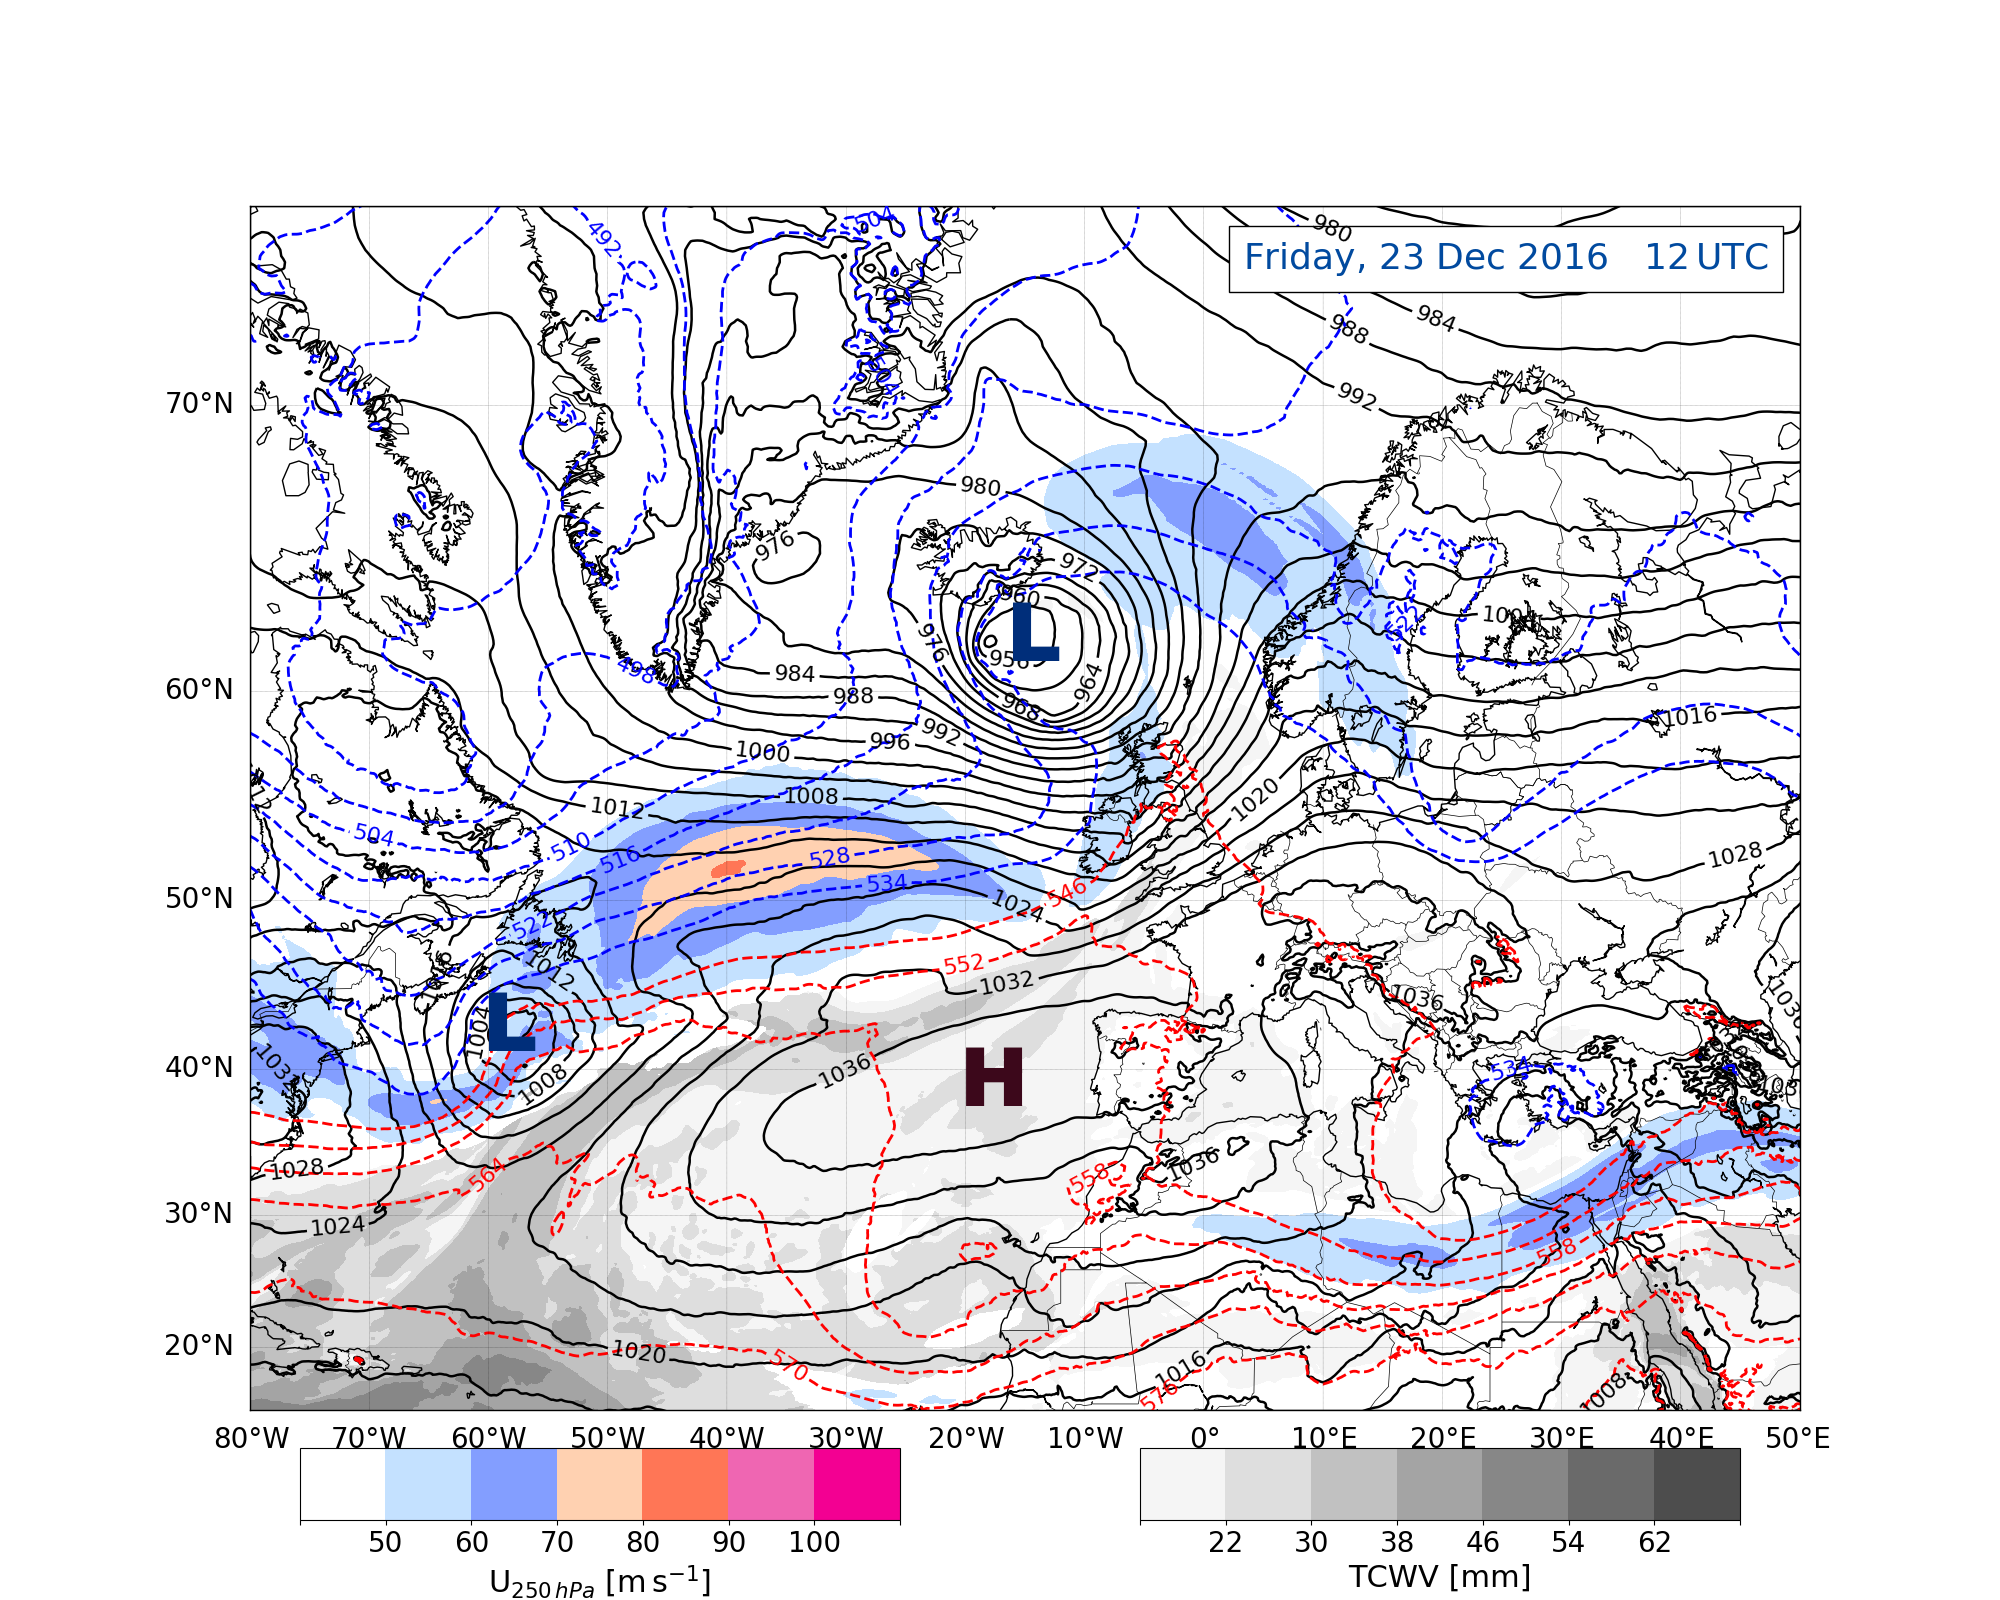
\includegraphics[trim={4.2cm 3.9cm 4.3cm 5.1cm},clip,
	width=\textwidth]{./fig_Geopot_Jet/20161223_12}
		\caption{}\label{fig:GP23}
	\end{subfigure}
%%%%%% label
    \begin{subfigure}[b]{\textwidth}
        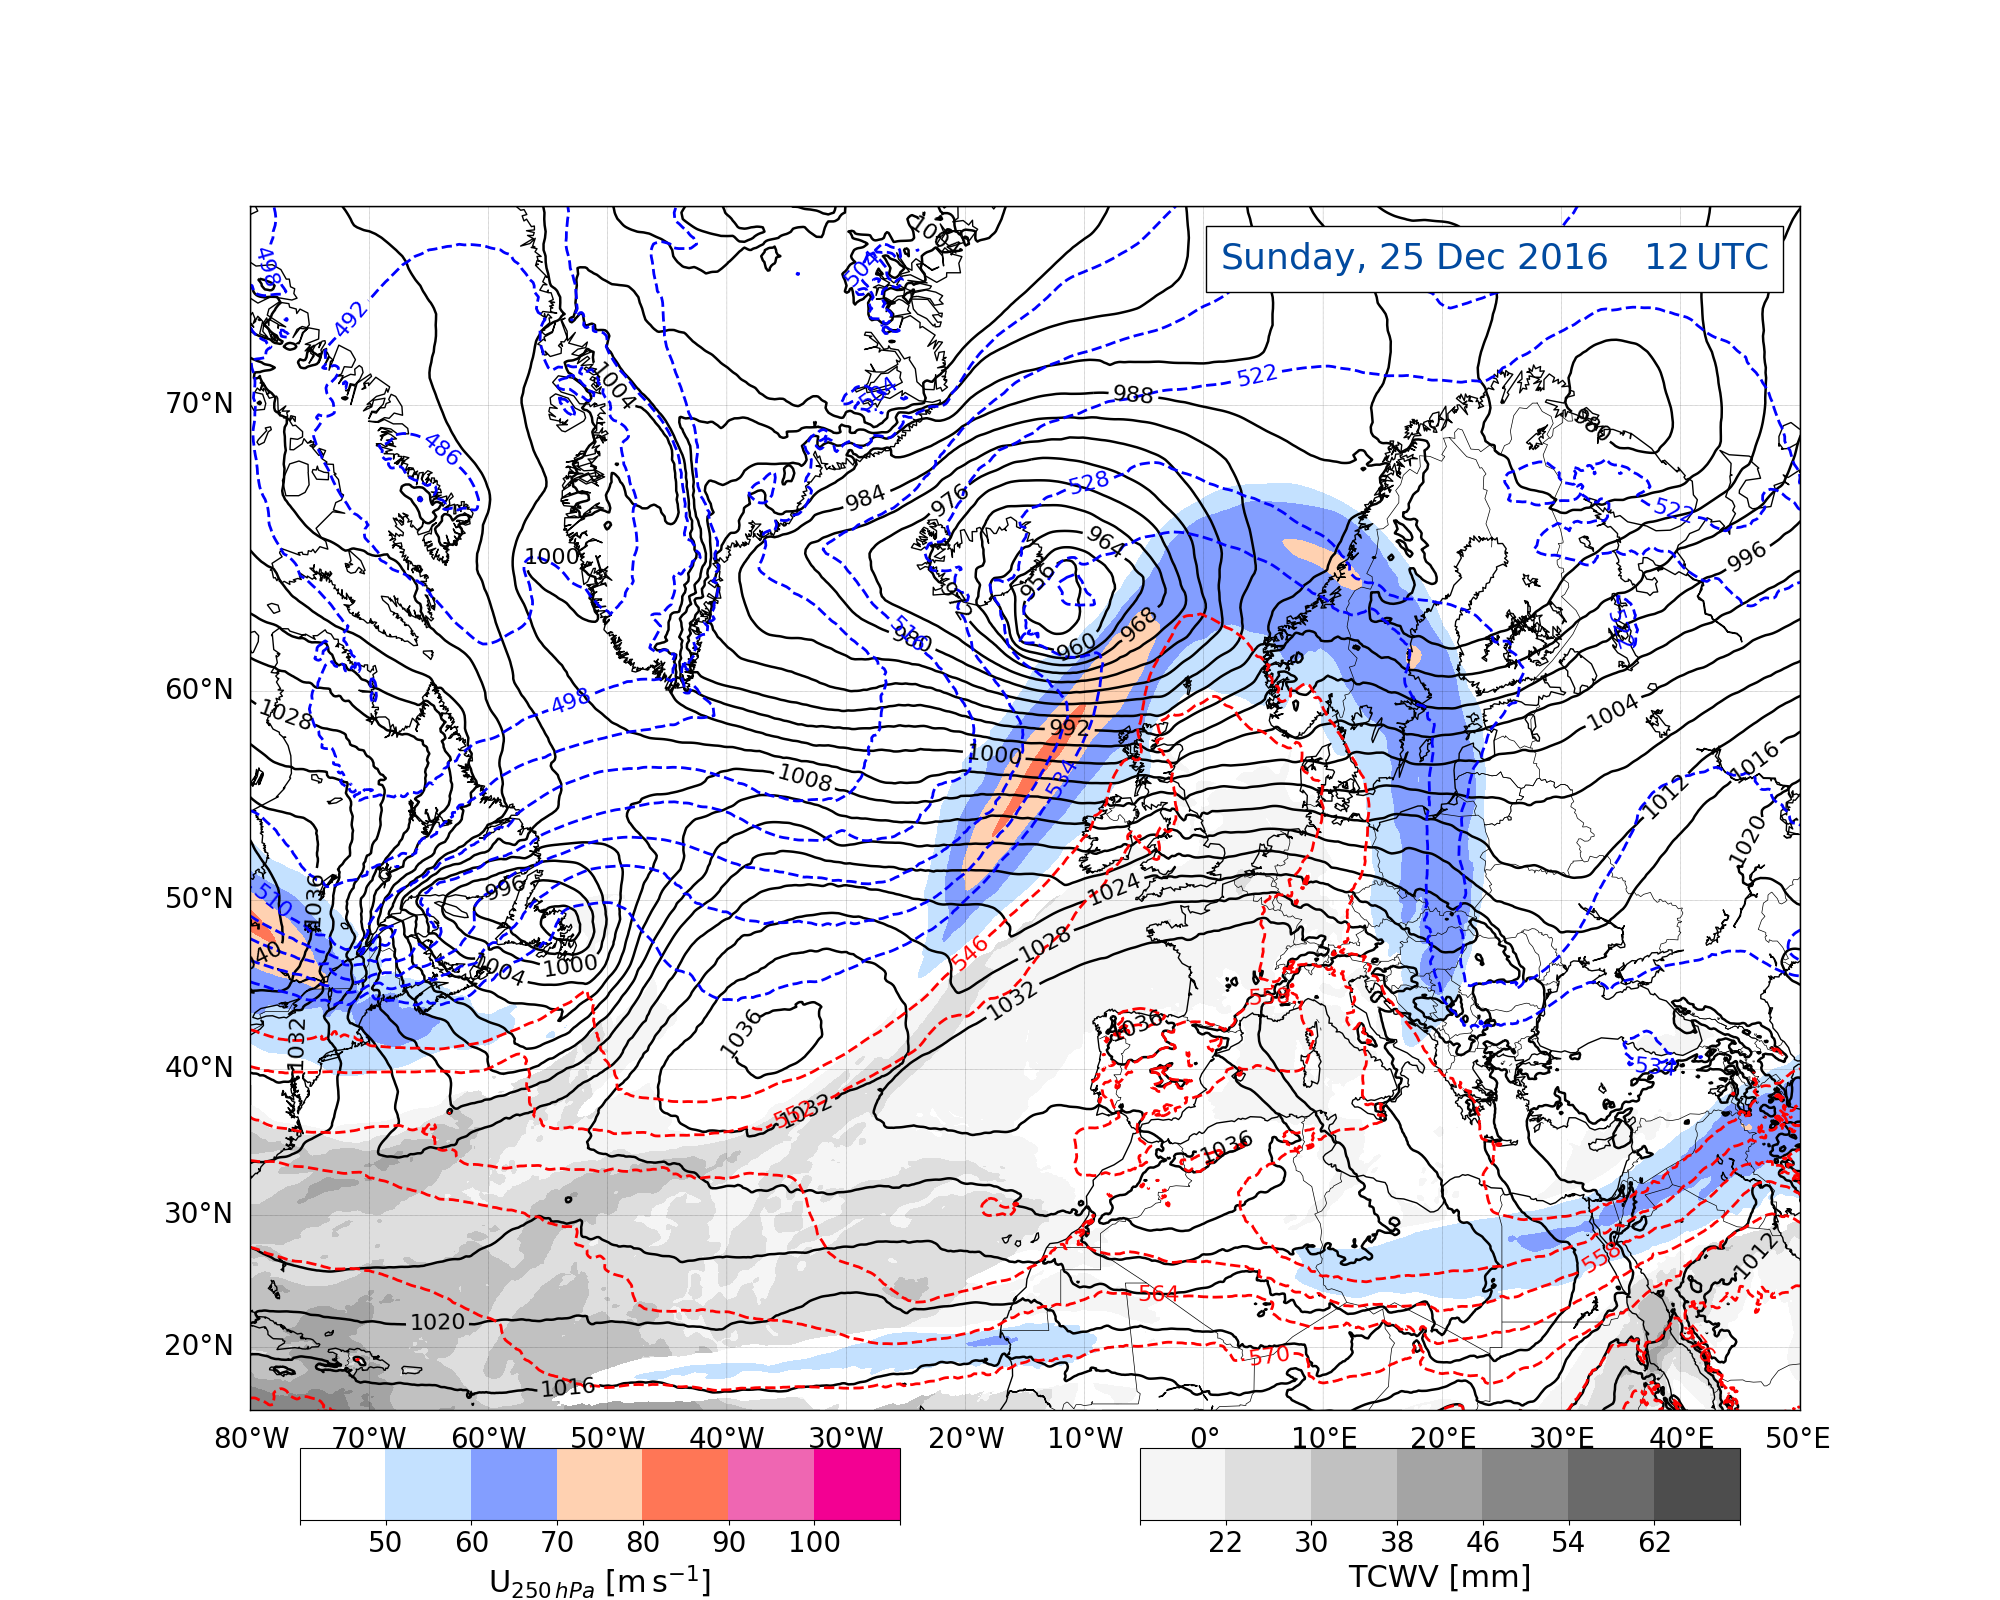
\includegraphics[trim={4.2cm 0cm 4.3cm 36.8cm},clip,
        width=\textwidth]{./fig_Geopot_Jet/20161225_12}
    \end{subfigure}
\caption{Jet, thickness, mean sea level pressure, and moisture synoptic analysis, data from ECMWF. During \SIrange{20}{27}{\dec}. \SI{250}{\hPa} wind speed, shaded according to the colour bar, [\SI{}{\mPs}]. \SI{1000}-\SI{500}{\hPa} thickness, dashed contours every \SI{6}{\deca\meter}, MSLP, black contours every \SI{4}{\hPa}, total column water vapour [\SI{}{\mm}], shaded according the grey scale.}\label{fig:GeopJet}
\end{figure}
\begin{figure}\ContinuedFloat
	\centering
%%%%%% 24/12
    \begin{subfigure}[b]{0.49\textwidth}
        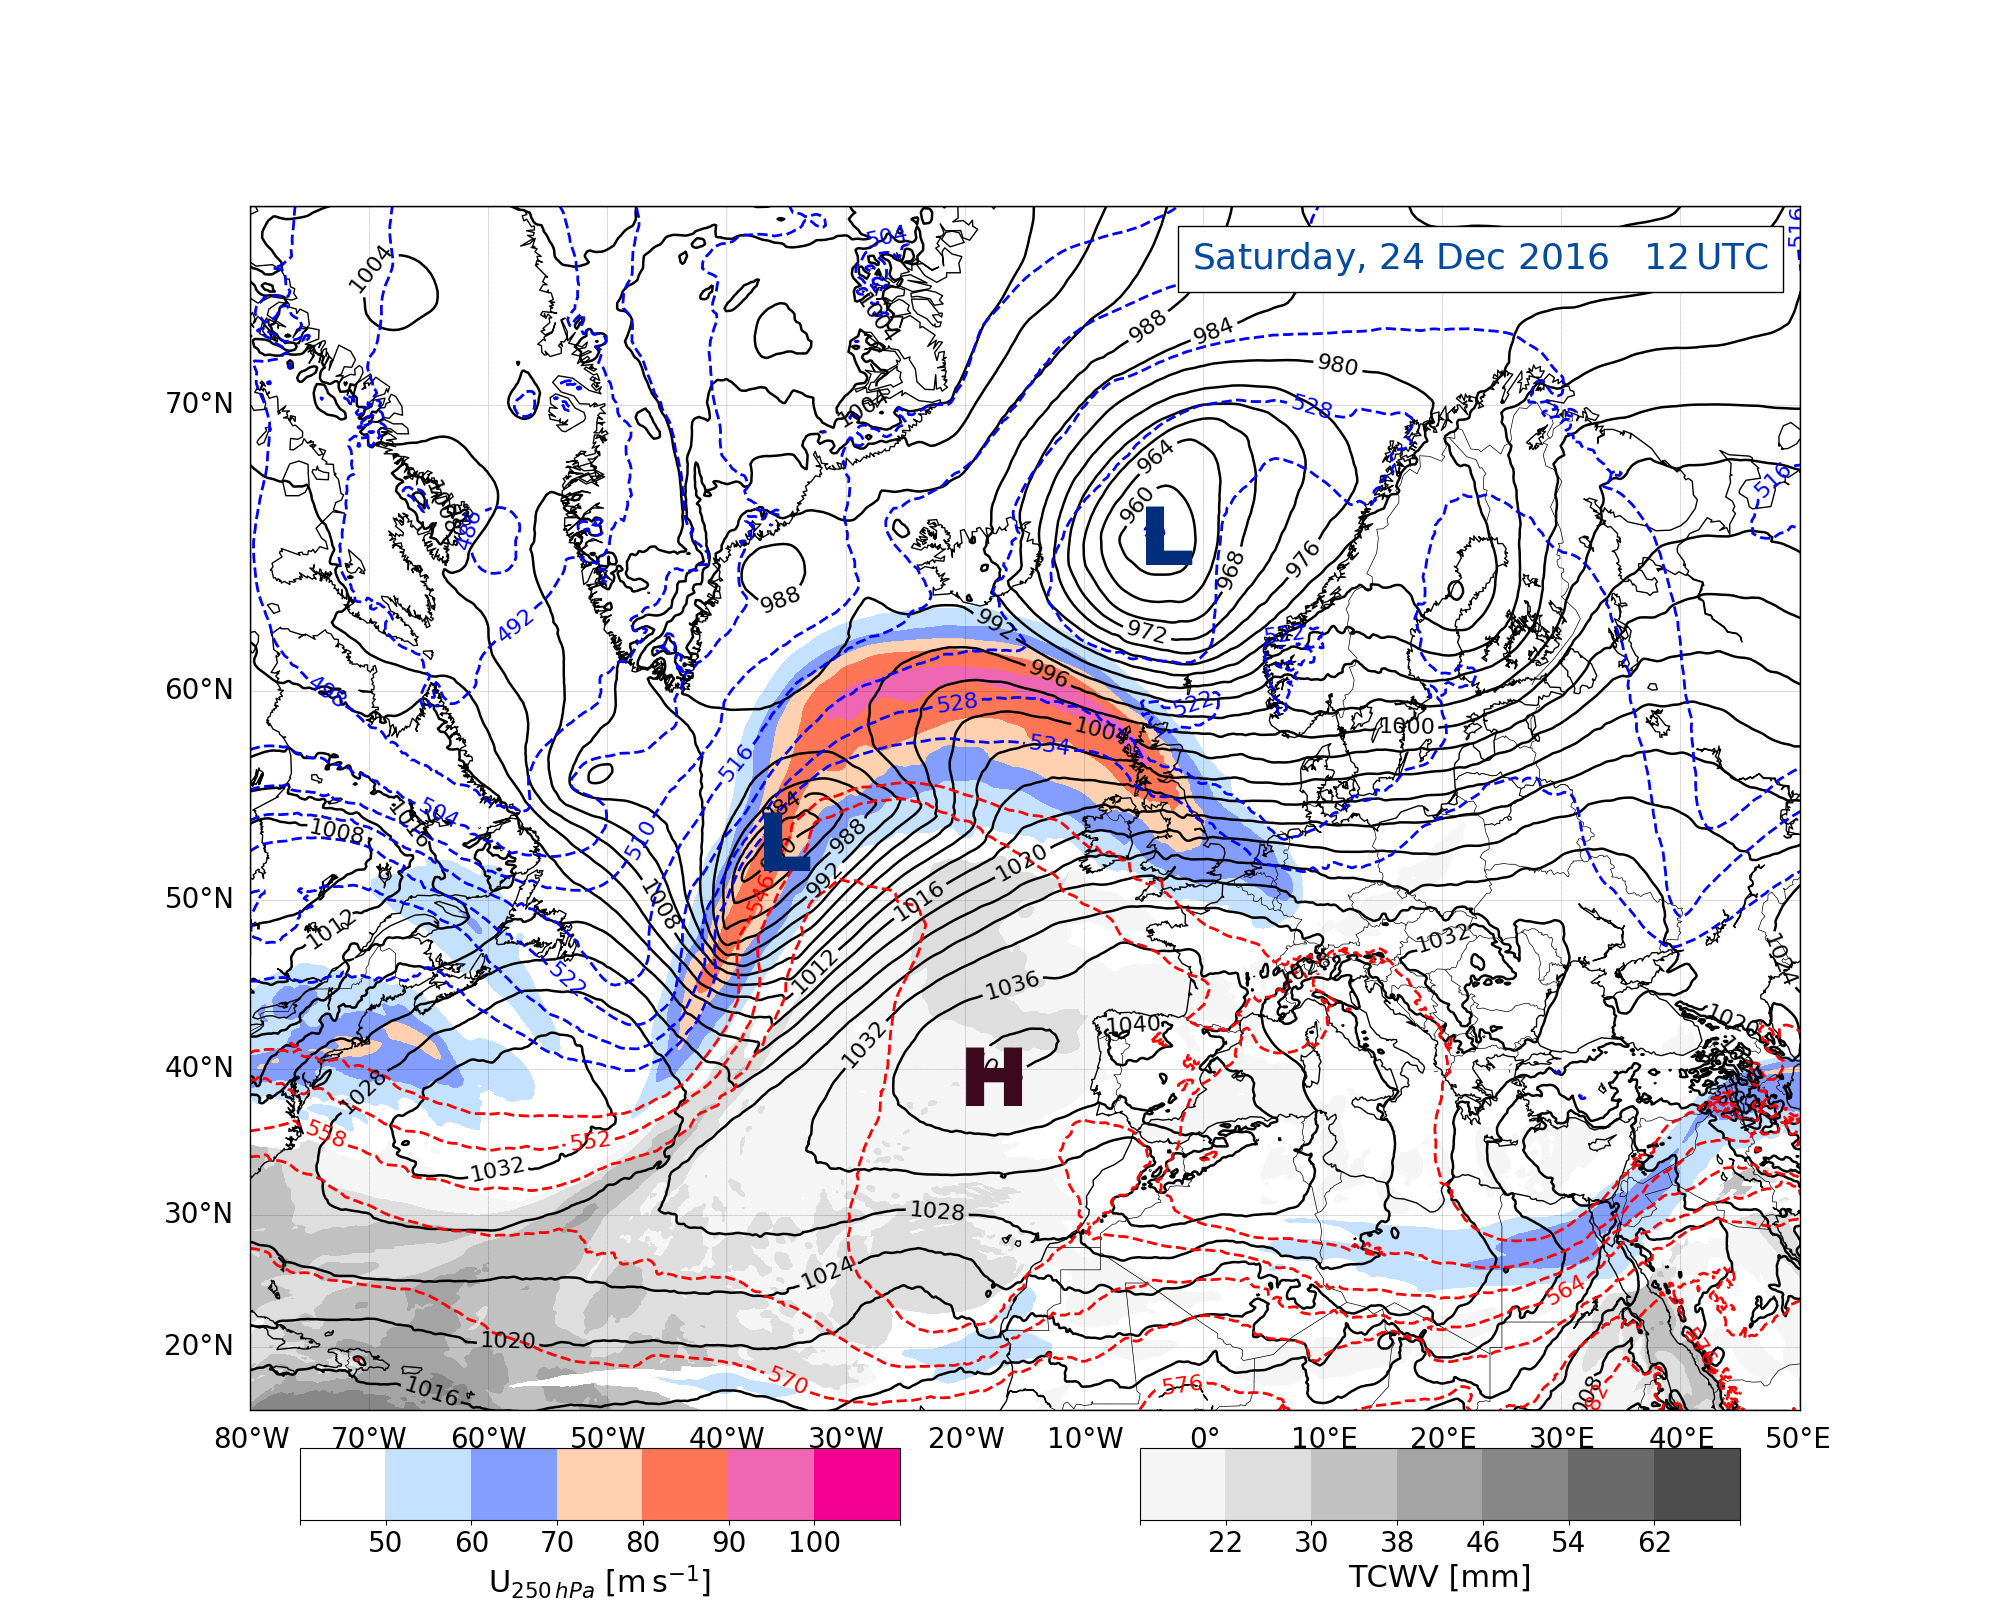
\includegraphics[trim={4.2cm 3.9cm 4.3cm 5.1cm},clip,
        width=\textwidth]{./fig_Geopot_Jet/20161224_12}
        \caption{}\label{fig:GP24}
    \end{subfigure}
%%%%%% 25/12
    \begin{subfigure}[b]{0.49\textwidth}
        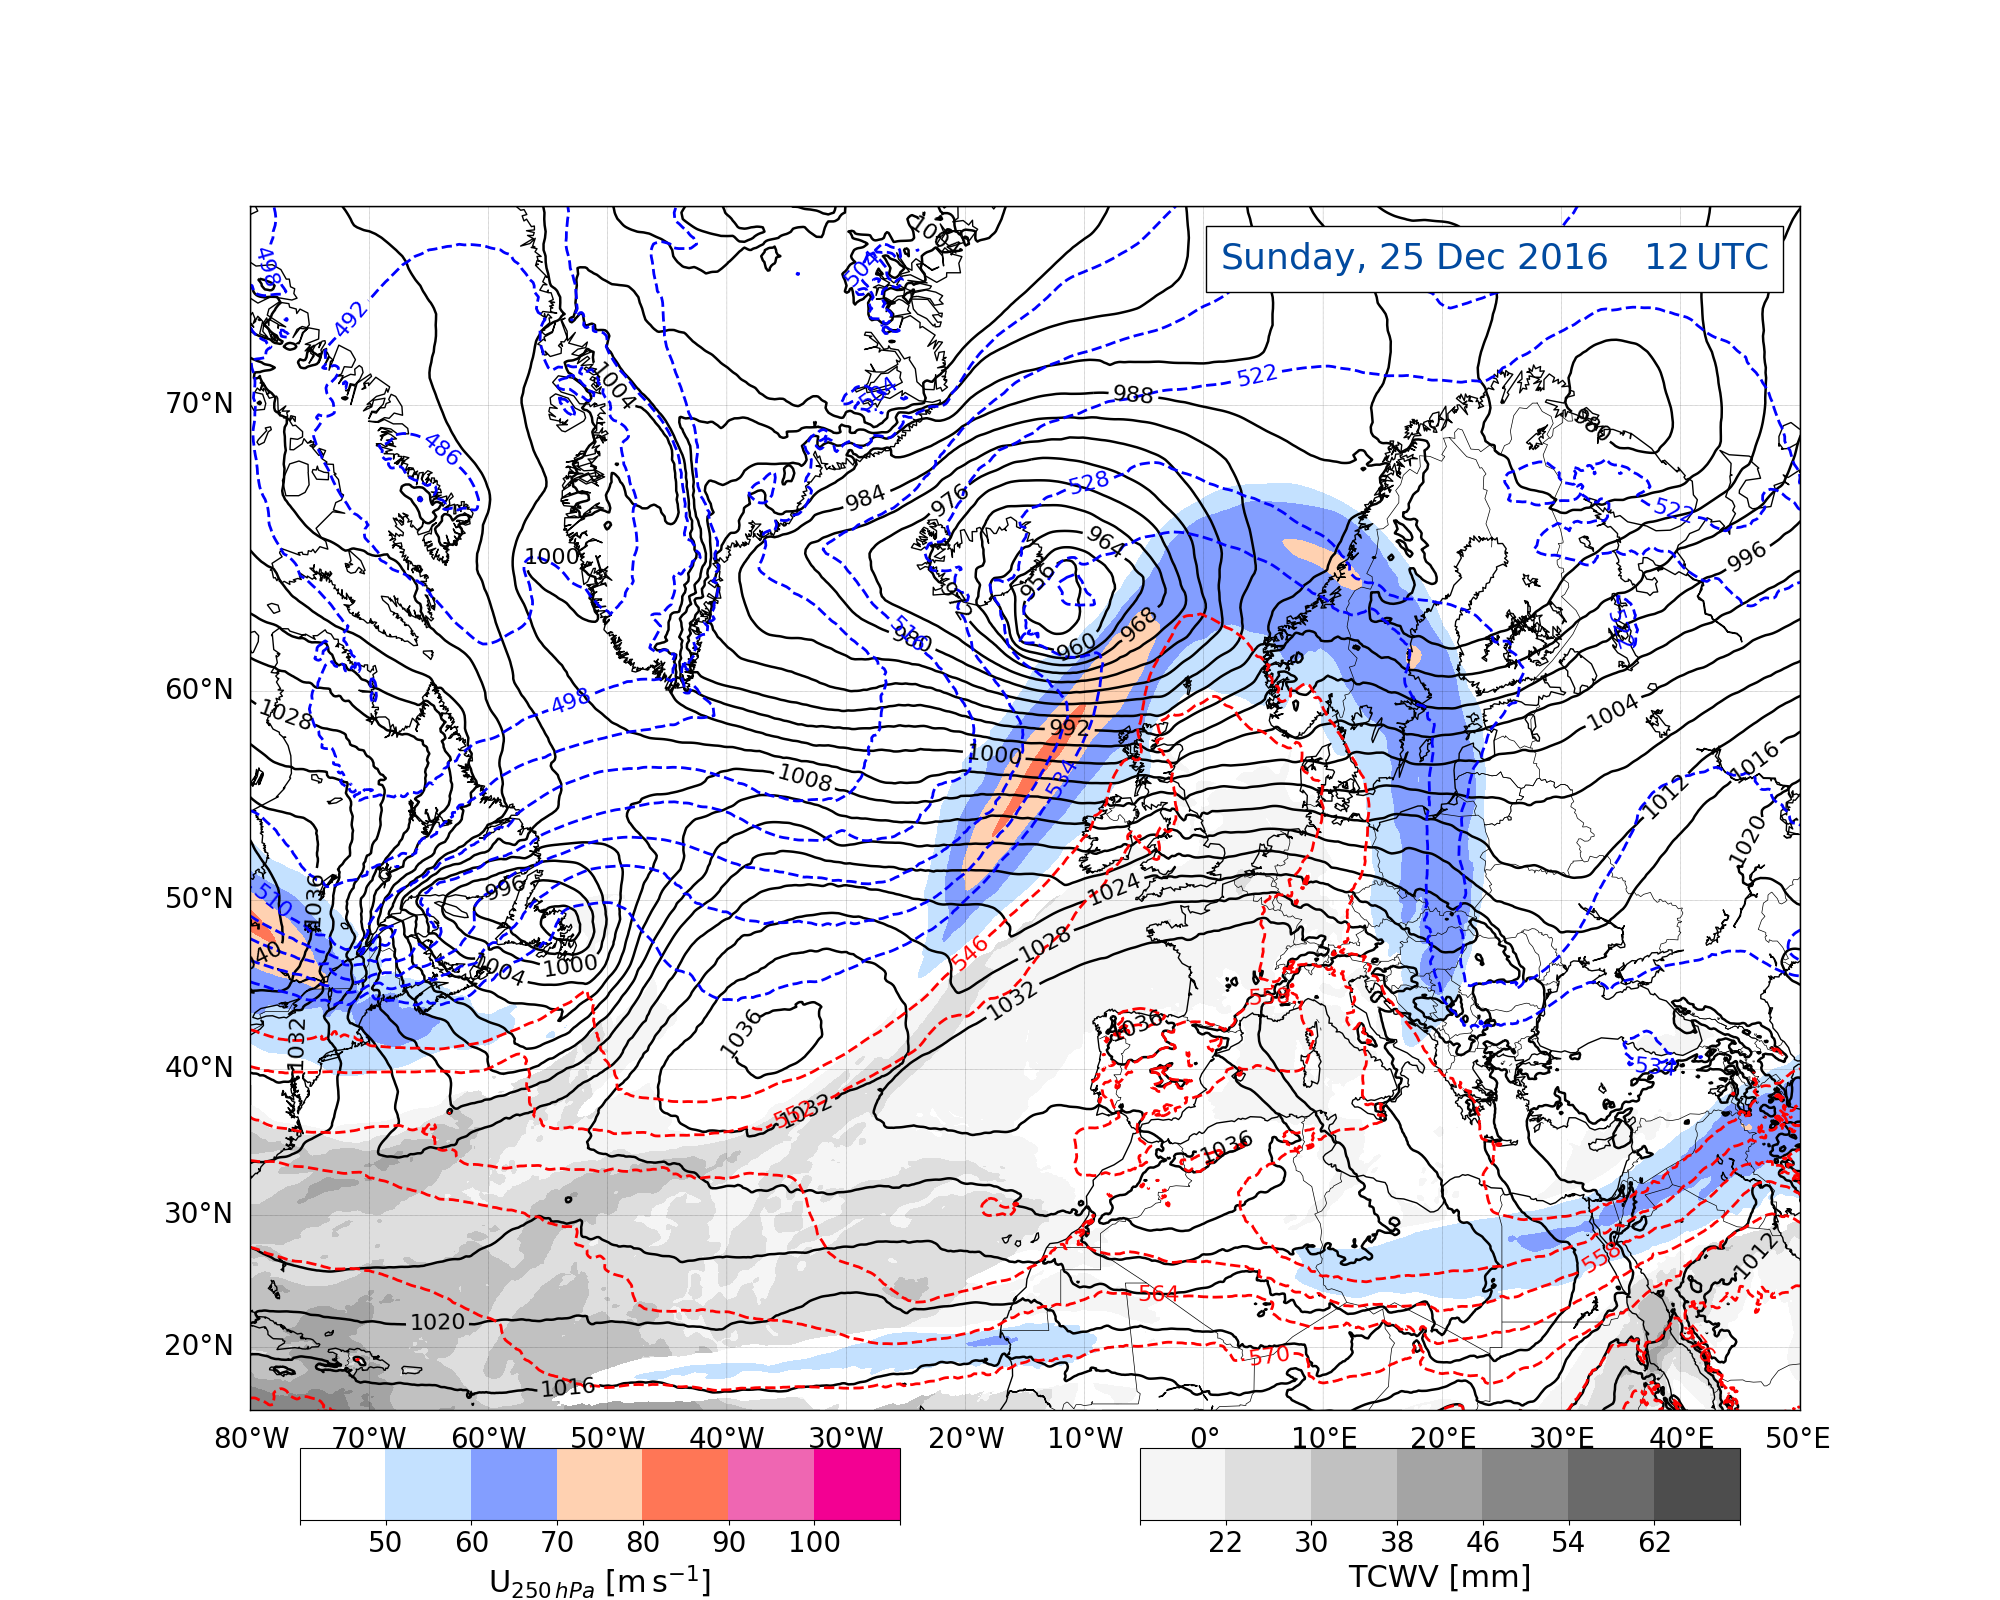
\includegraphics[trim={4.2cm 3.9cm 4.3cm 5.1cm},clip,
        width=\textwidth]{./fig_Geopot_Jet/20161225_12}
        \caption{}\label{fig:GP25}
    \end{subfigure}
%	\centering
%%%%%% 26/12
    \begin{subfigure}[b]{0.49\textwidth}
        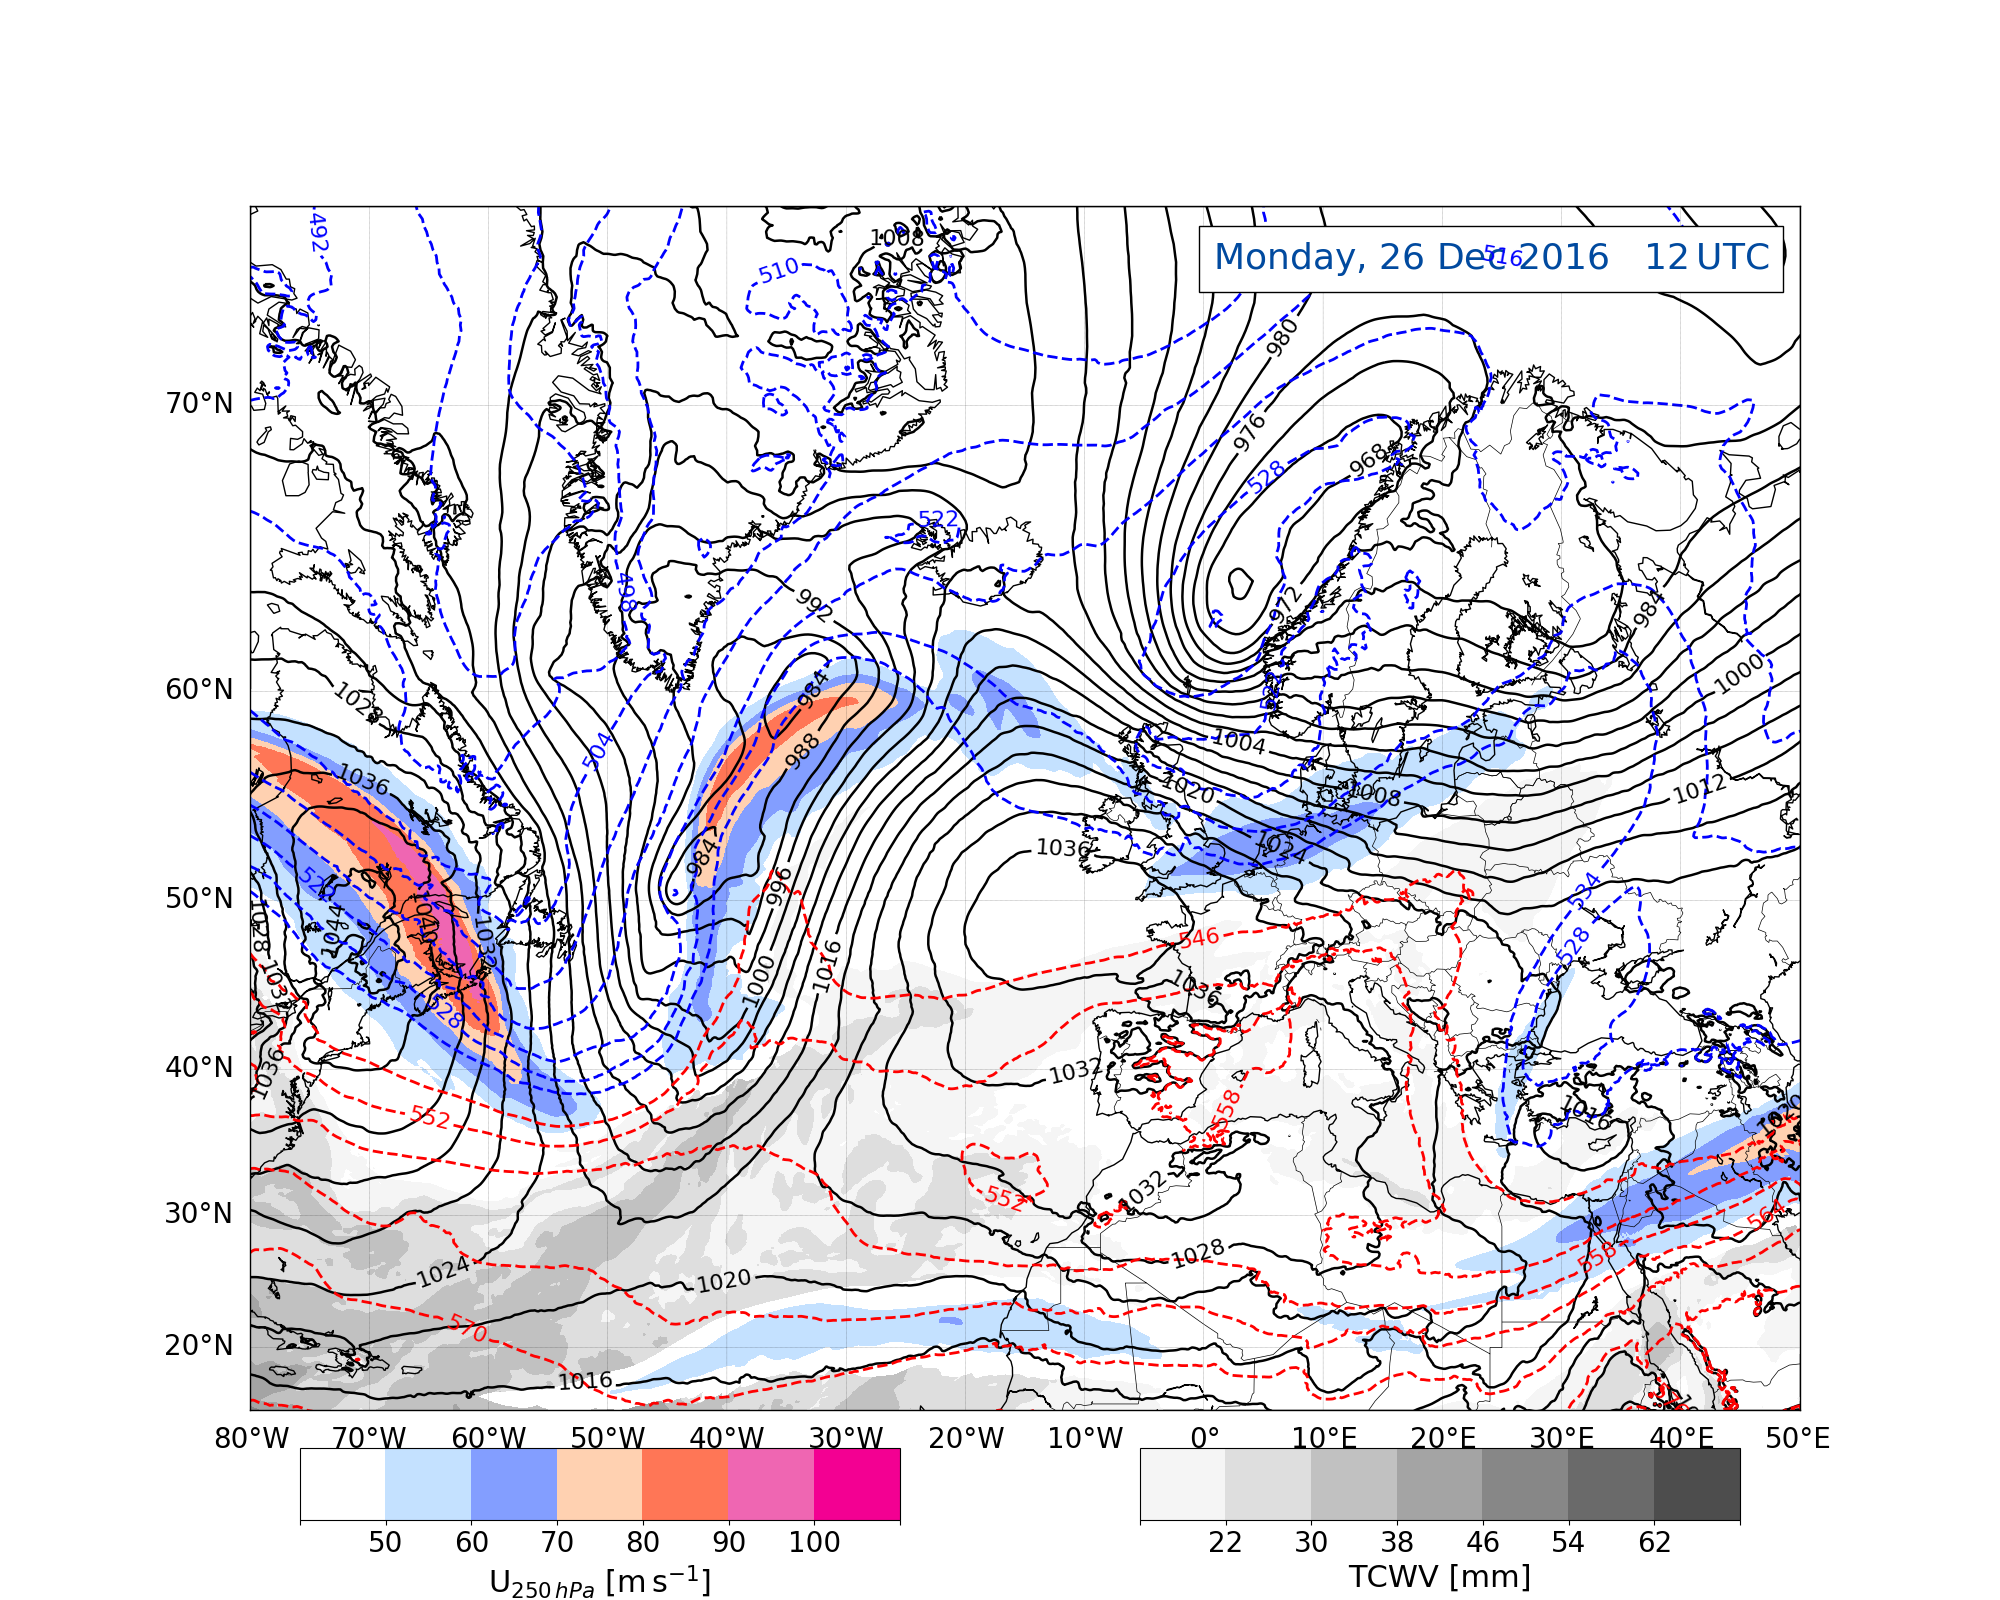
\includegraphics[trim={4.2cm 3.9cm 4.3cm 5.1cm},clip,
        width=\textwidth]{./fig_Geopot_Jet/20161226_12}
        \caption{}\label{fig:GP26}
    \end{subfigure}
%%%%%% 27/12
    \begin{subfigure}[b]{0.49\textwidth}
        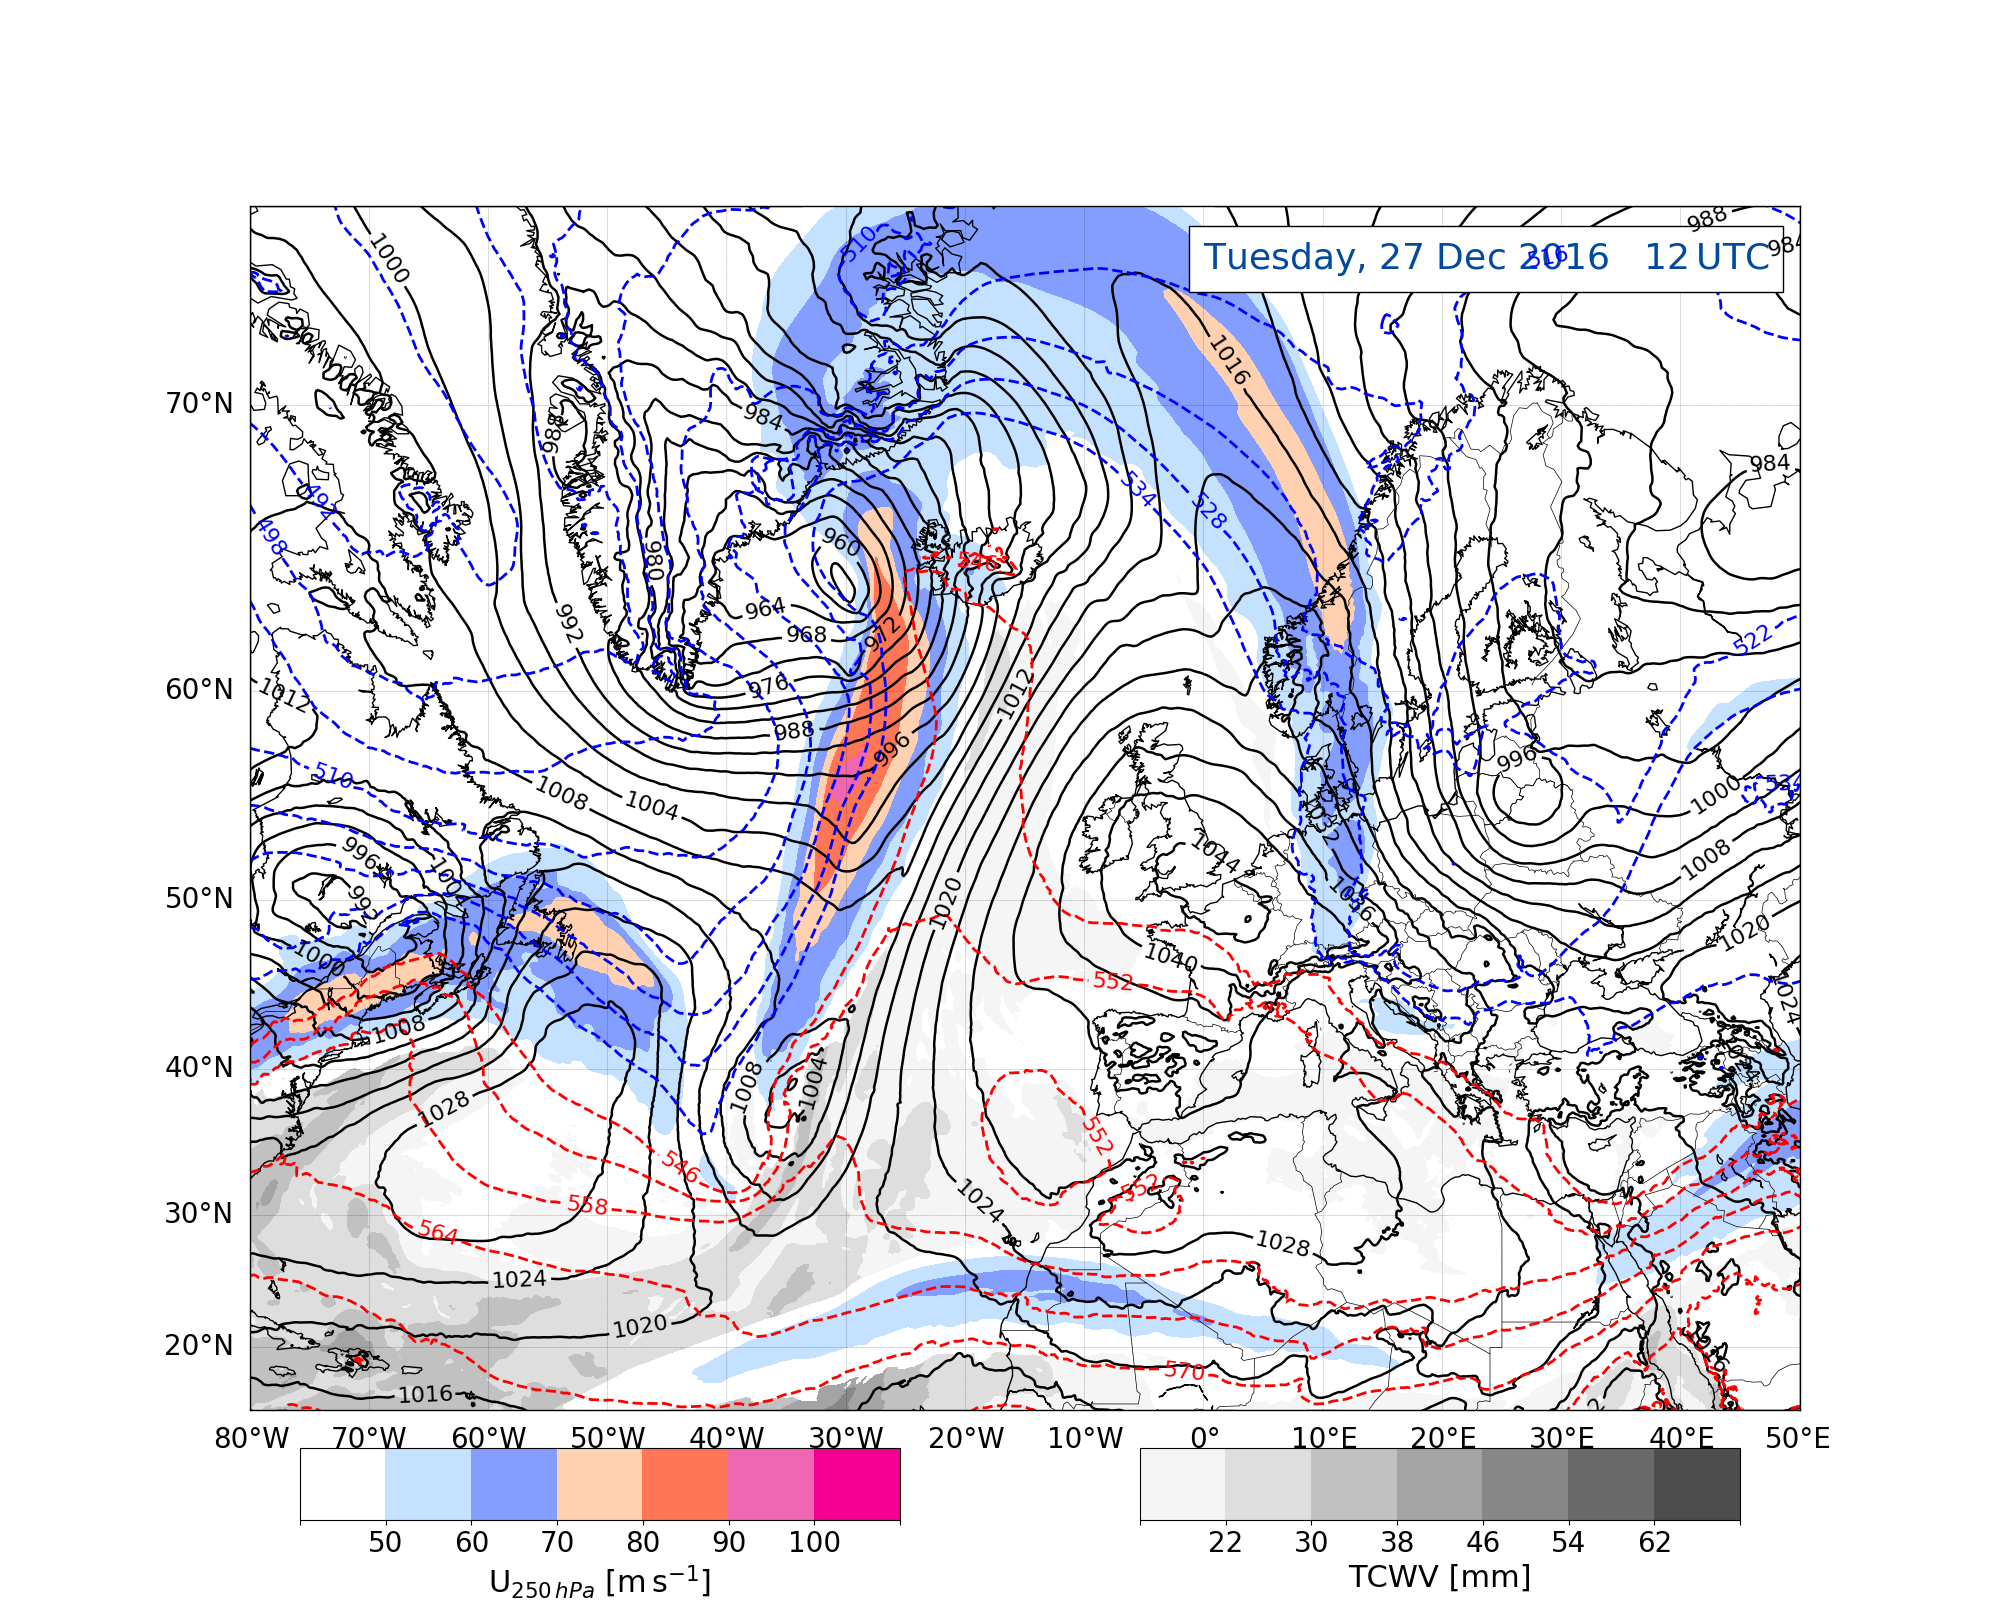
\includegraphics[trim={4.2cm 3.9cm 4.3cm 5.1cm},clip,
        width=\textwidth]{./fig_Geopot_Jet/20161227_12}
        \caption{}\label{fig:GP27}
    \end{subfigure}
%%%%%% label
    \begin{subfigure}[b]{\textwidth}
        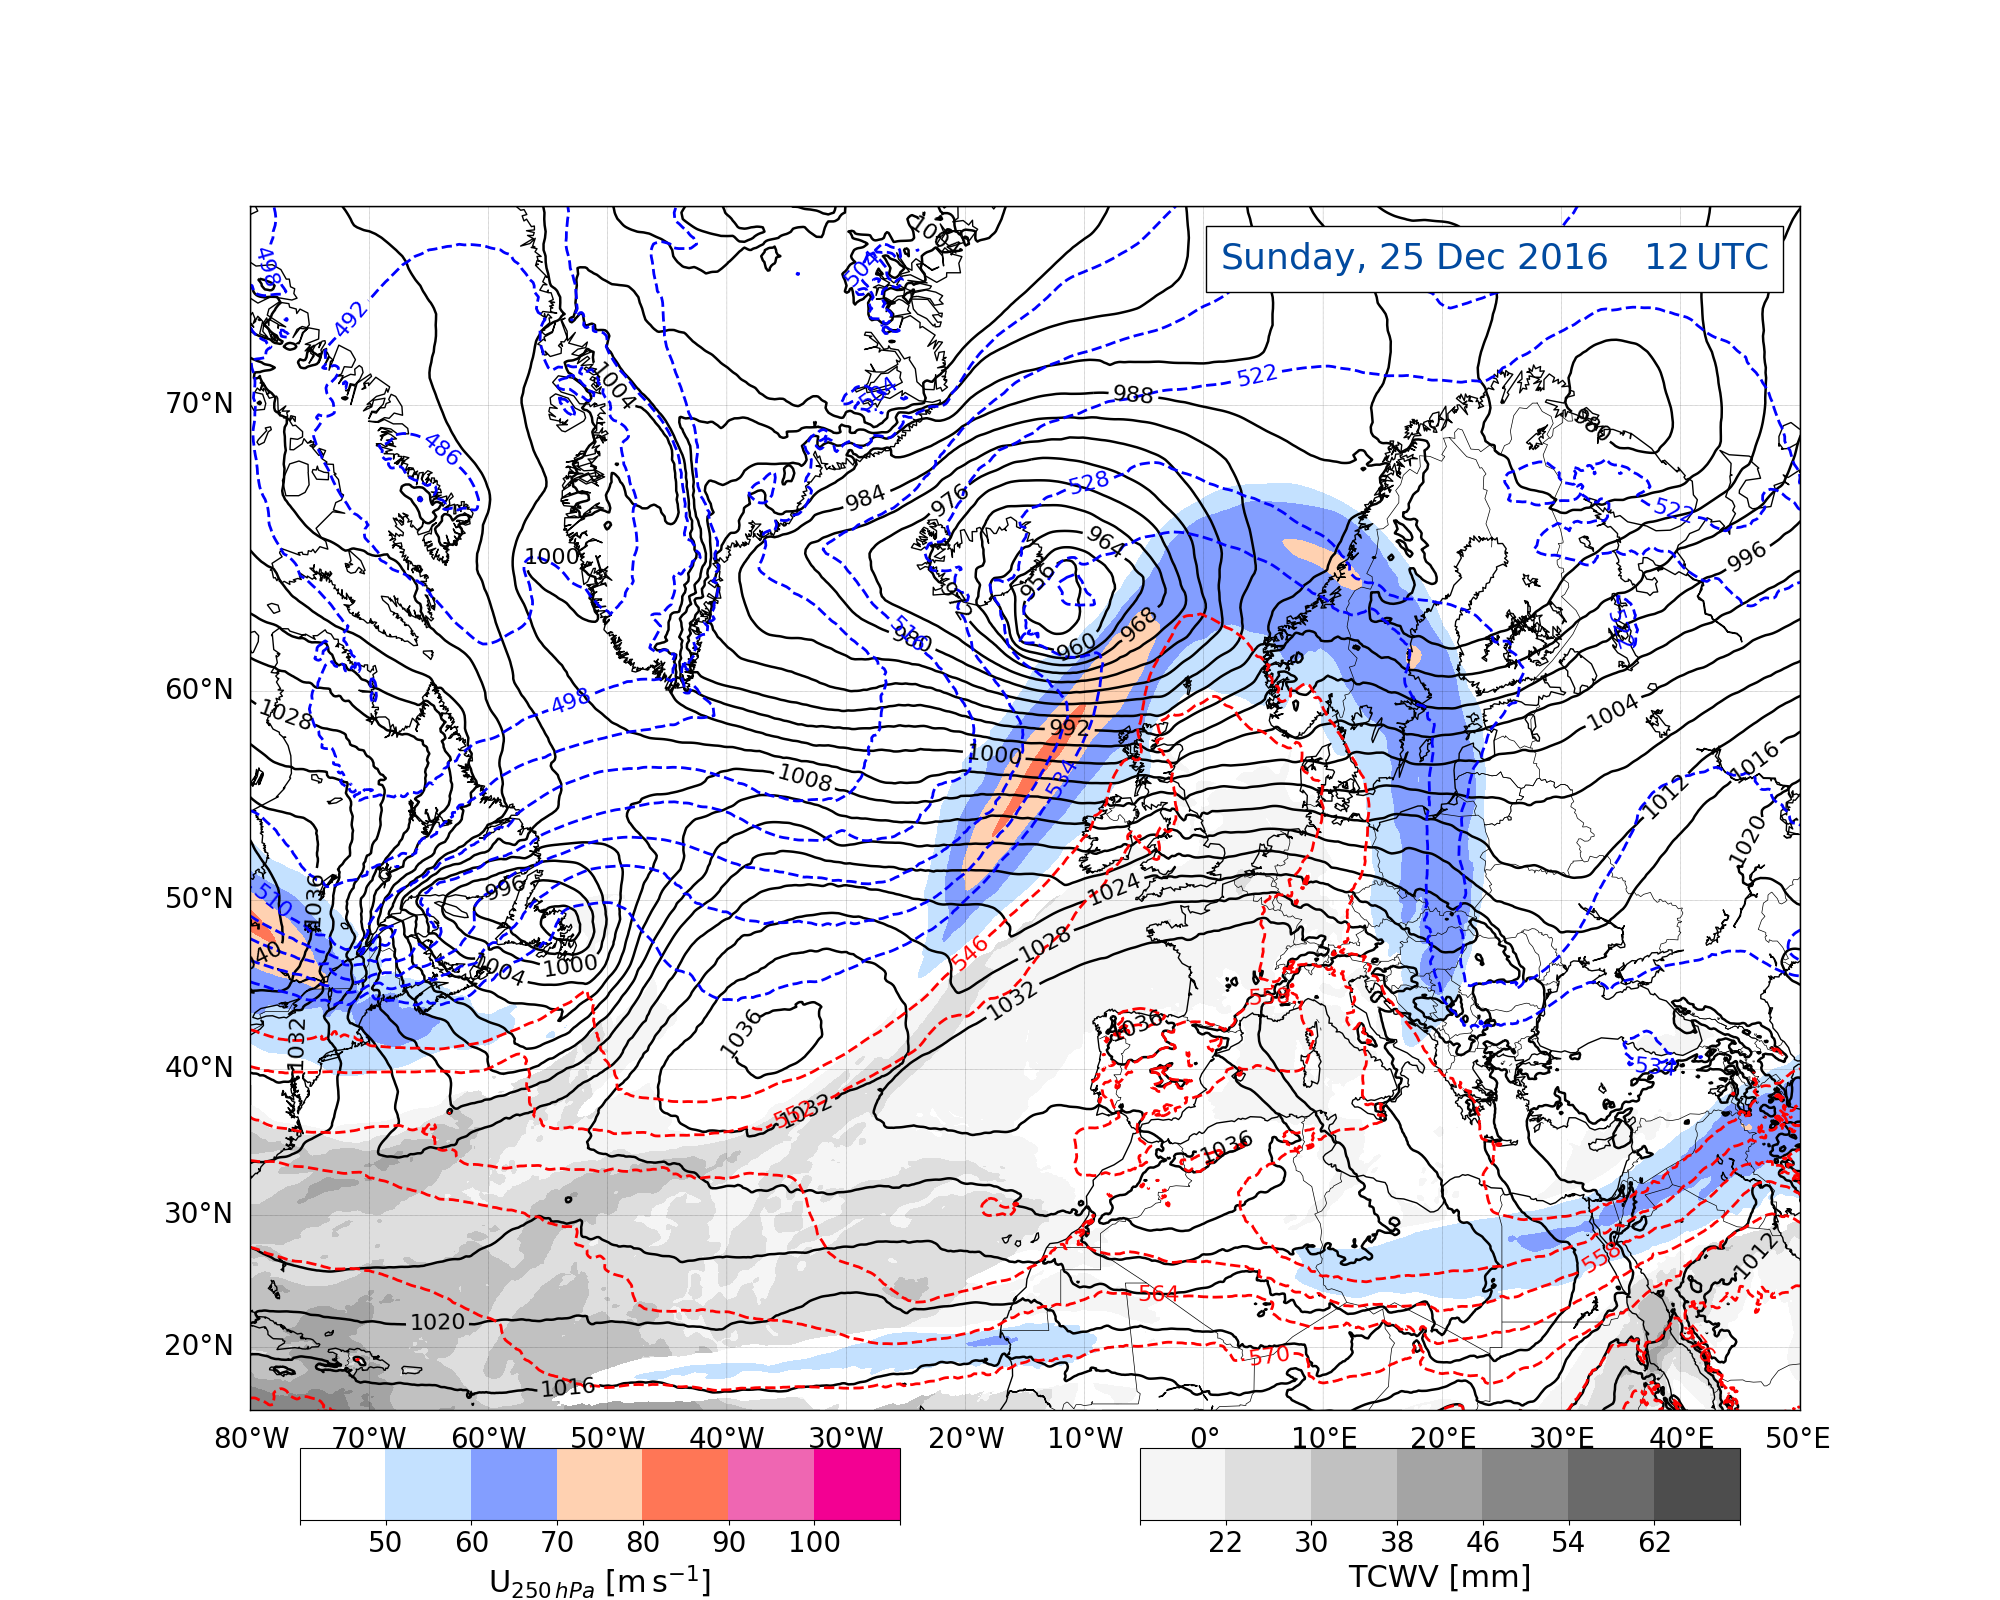
\includegraphics[trim={4.2cm 0cm 4.3cm 36.8cm},clip,
        width=\textwidth]{./fig_Geopot_Jet/20161225_12}
       % \label{fig:D}
    \end{subfigure}
\caption{\textit{(Continued from previous page.)}}   
\end{figure}
% %%%%%%%%%%%%%%%%%%%%%%%%%%%%%%%%%%%%%%%%%%%%%%%%%%%%%%%%%%%%%%%%%%%%%%%%%%
%\noindent 
\\
The dashed, coloured contours in \Cref{fig:GP24_pres} show the vertical thickness between the \SI{1000}{\hPa} and \SI{500}{\hPa} surface, every \SI{6}{\deca\meter}. The thickness between two pressure levels can be interpreted via the hypsometric equation (\Cref{eq:hypsometric}), which equates the thickness to the mean temperature of the layer in question. In a relative sense, a larger thickness indicates a warmer air mass. In addition, strong horizontal gradients in the thickness field can be related to frontal boundaries. Specific to the discussion in this thesis, the thickness field also provides useful information regarding the form of precipitation (liquid, frozen).
%This is a relation of the mean temperature of the air between two pressure levels. Thus, high values of thickness mean relative warm, moist air (red, dashed). This can then be associated to rain or snow in mid-latitudes, depending on cold or warm air advection.
\\
%Gray shaded areas describe total precipitable water in the atmosphere in \SI{}{\mm}. 
Analysis of the mean sea level pressure can be used to identify cyclones (L) and anticyclones (H) at the surface as well as provide supplementary information regarding frontal boundaries (\Cref{fig:GP24_pres}).
The total precipitable water is a measure of the column integrated moisture. It represents an instantaneous measure of moisture in time and space, which can be useful when assessing the amount of moisture that may fall as precipitation in future time steps.
The \SI{250}{\hPa} wind speeds are used to identify strong upper-level flow (i.e. the jet stream) and can be directly compared to the dynamic tropopause map (\Cref{fig:DT24_pres}).
% It is an indicator for the amount of moisture to supply rainfall, and will be used to identify where moisture was present.
% \\
% Colour shaded contours in \Cref{fig:GeopJet} indicate the mid-latitudal jet streaks at \SI{250}{\hPa}. Warmer colour is associated with higher wind speeds at this level.  

% %% Geopot Jet maps %%%%%%%%%%%%%%%%%%%%%%%%%%%%%%%%%%%%%
% % !TeX spellcheck = en_GB

\begin{figure}[h!]
    \centering
%%%%%% 20/12
    \begin{subfigure}[b]{0.49\textwidth}
        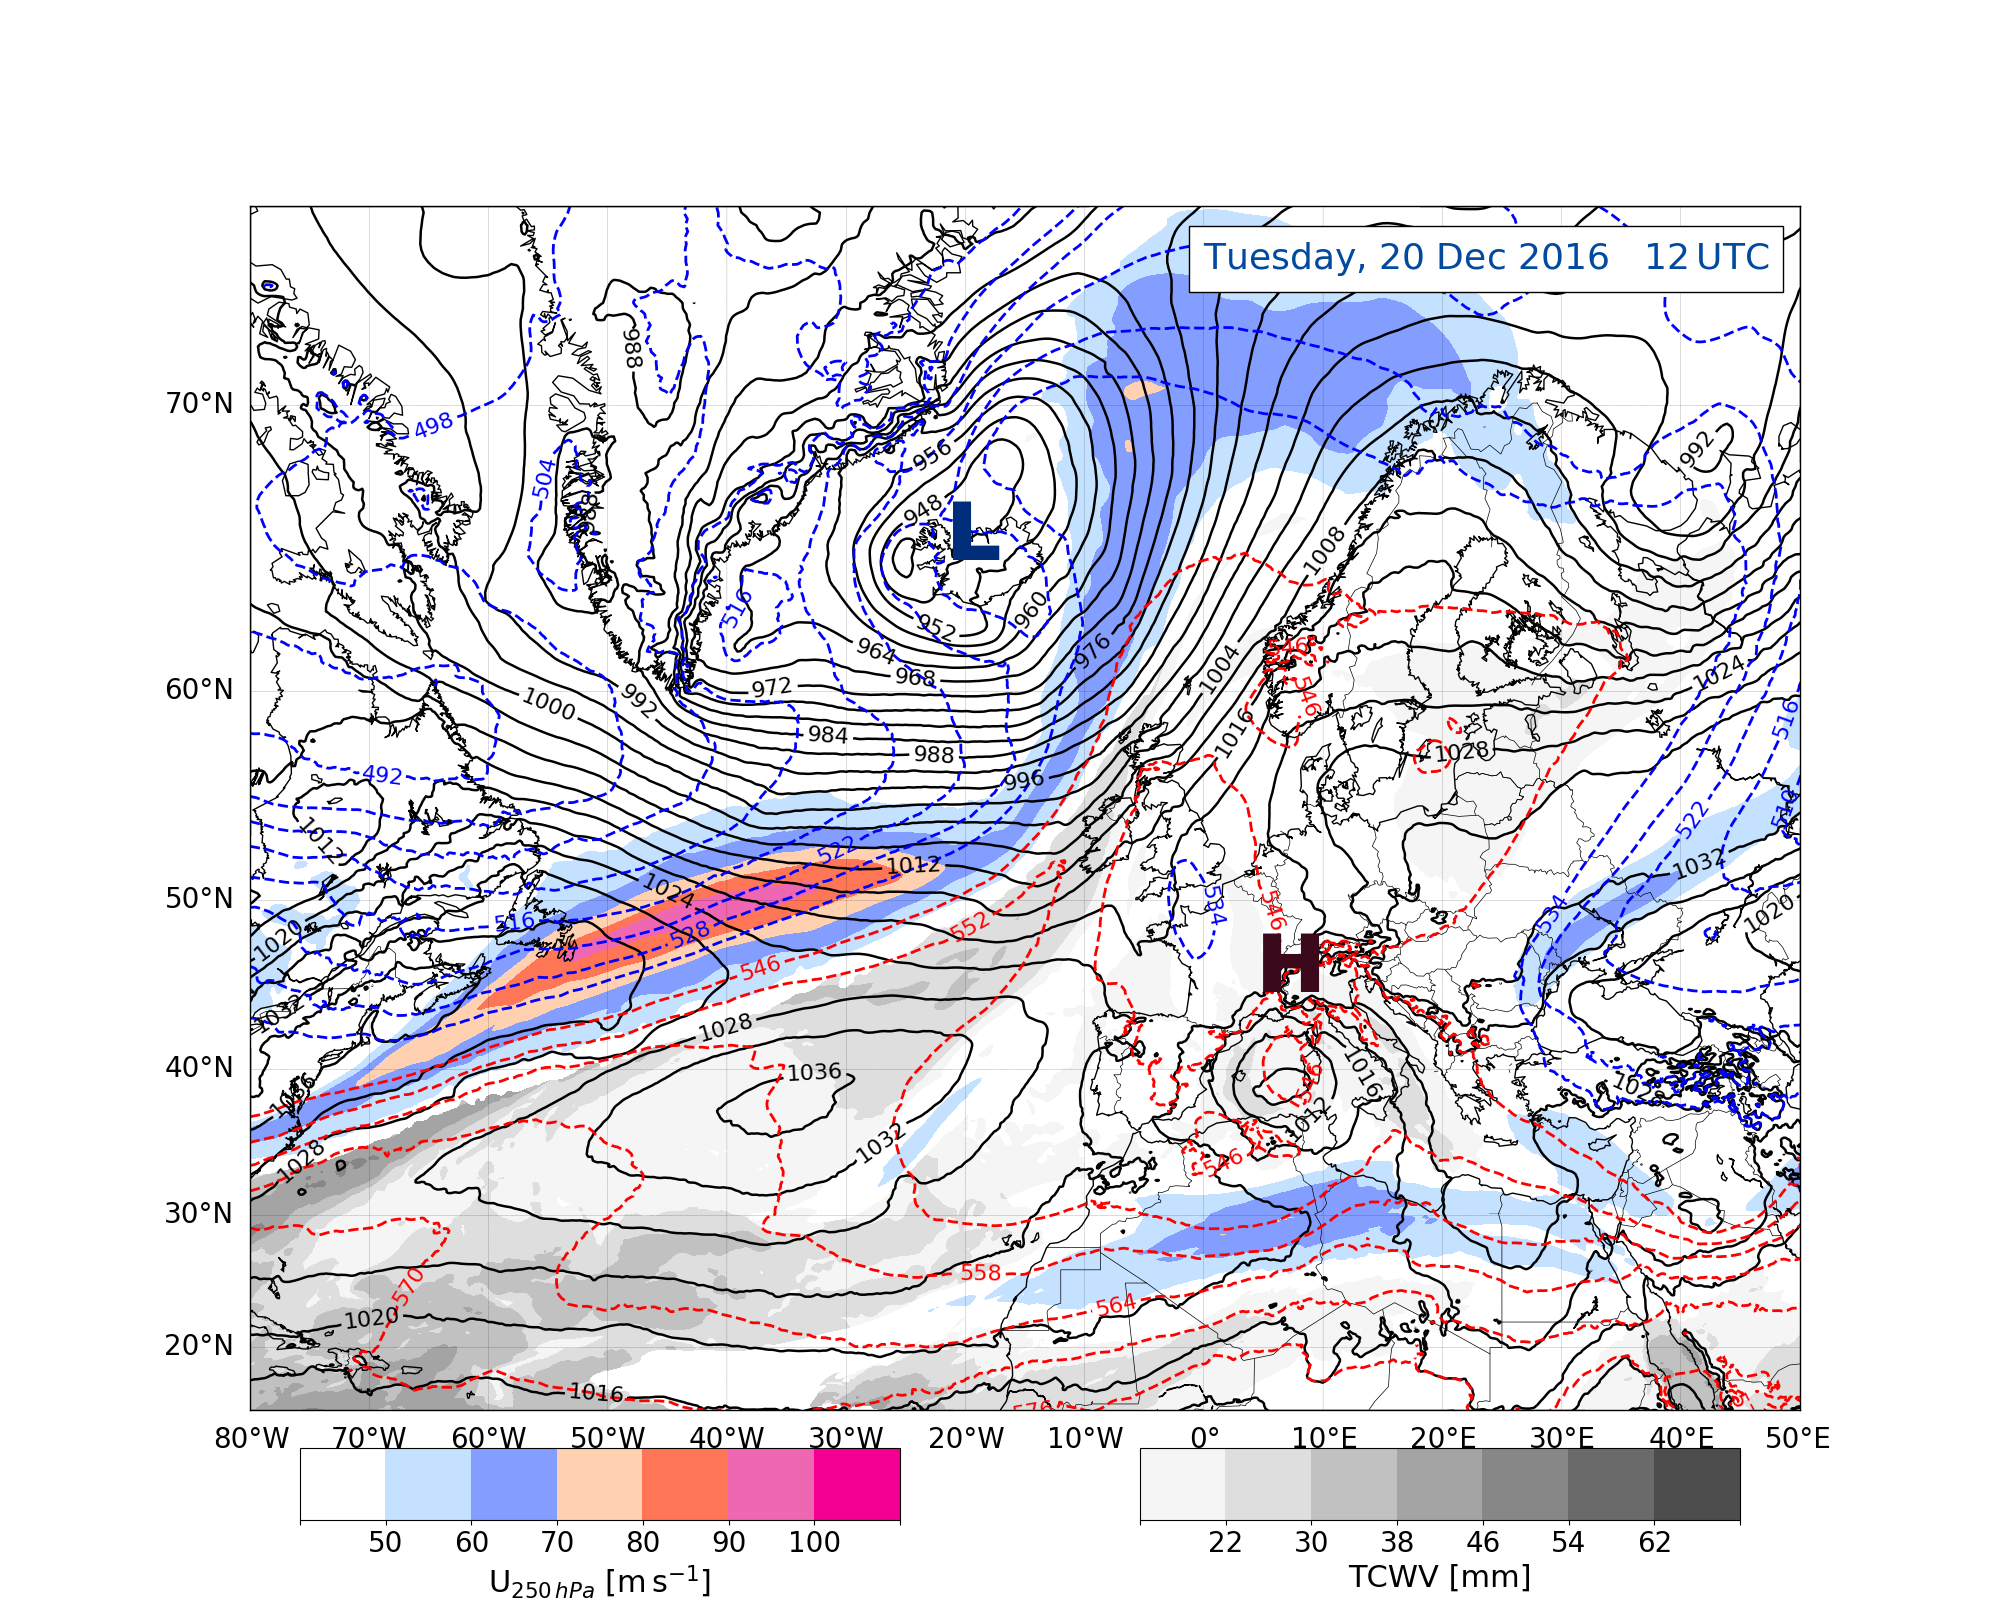
\includegraphics[trim={4.2cm 3.9cm 4.3cm 5.1cm},clip,
        width=\textwidth]{./fig_Geopot_Jet/20161220_12}
        \caption{}\label{fig:GP20}
        %\label{fig:DT2100}
    \end{subfigure}
%%%%%% 21/12
    \begin{subfigure}[b]{0.49\textwidth}
        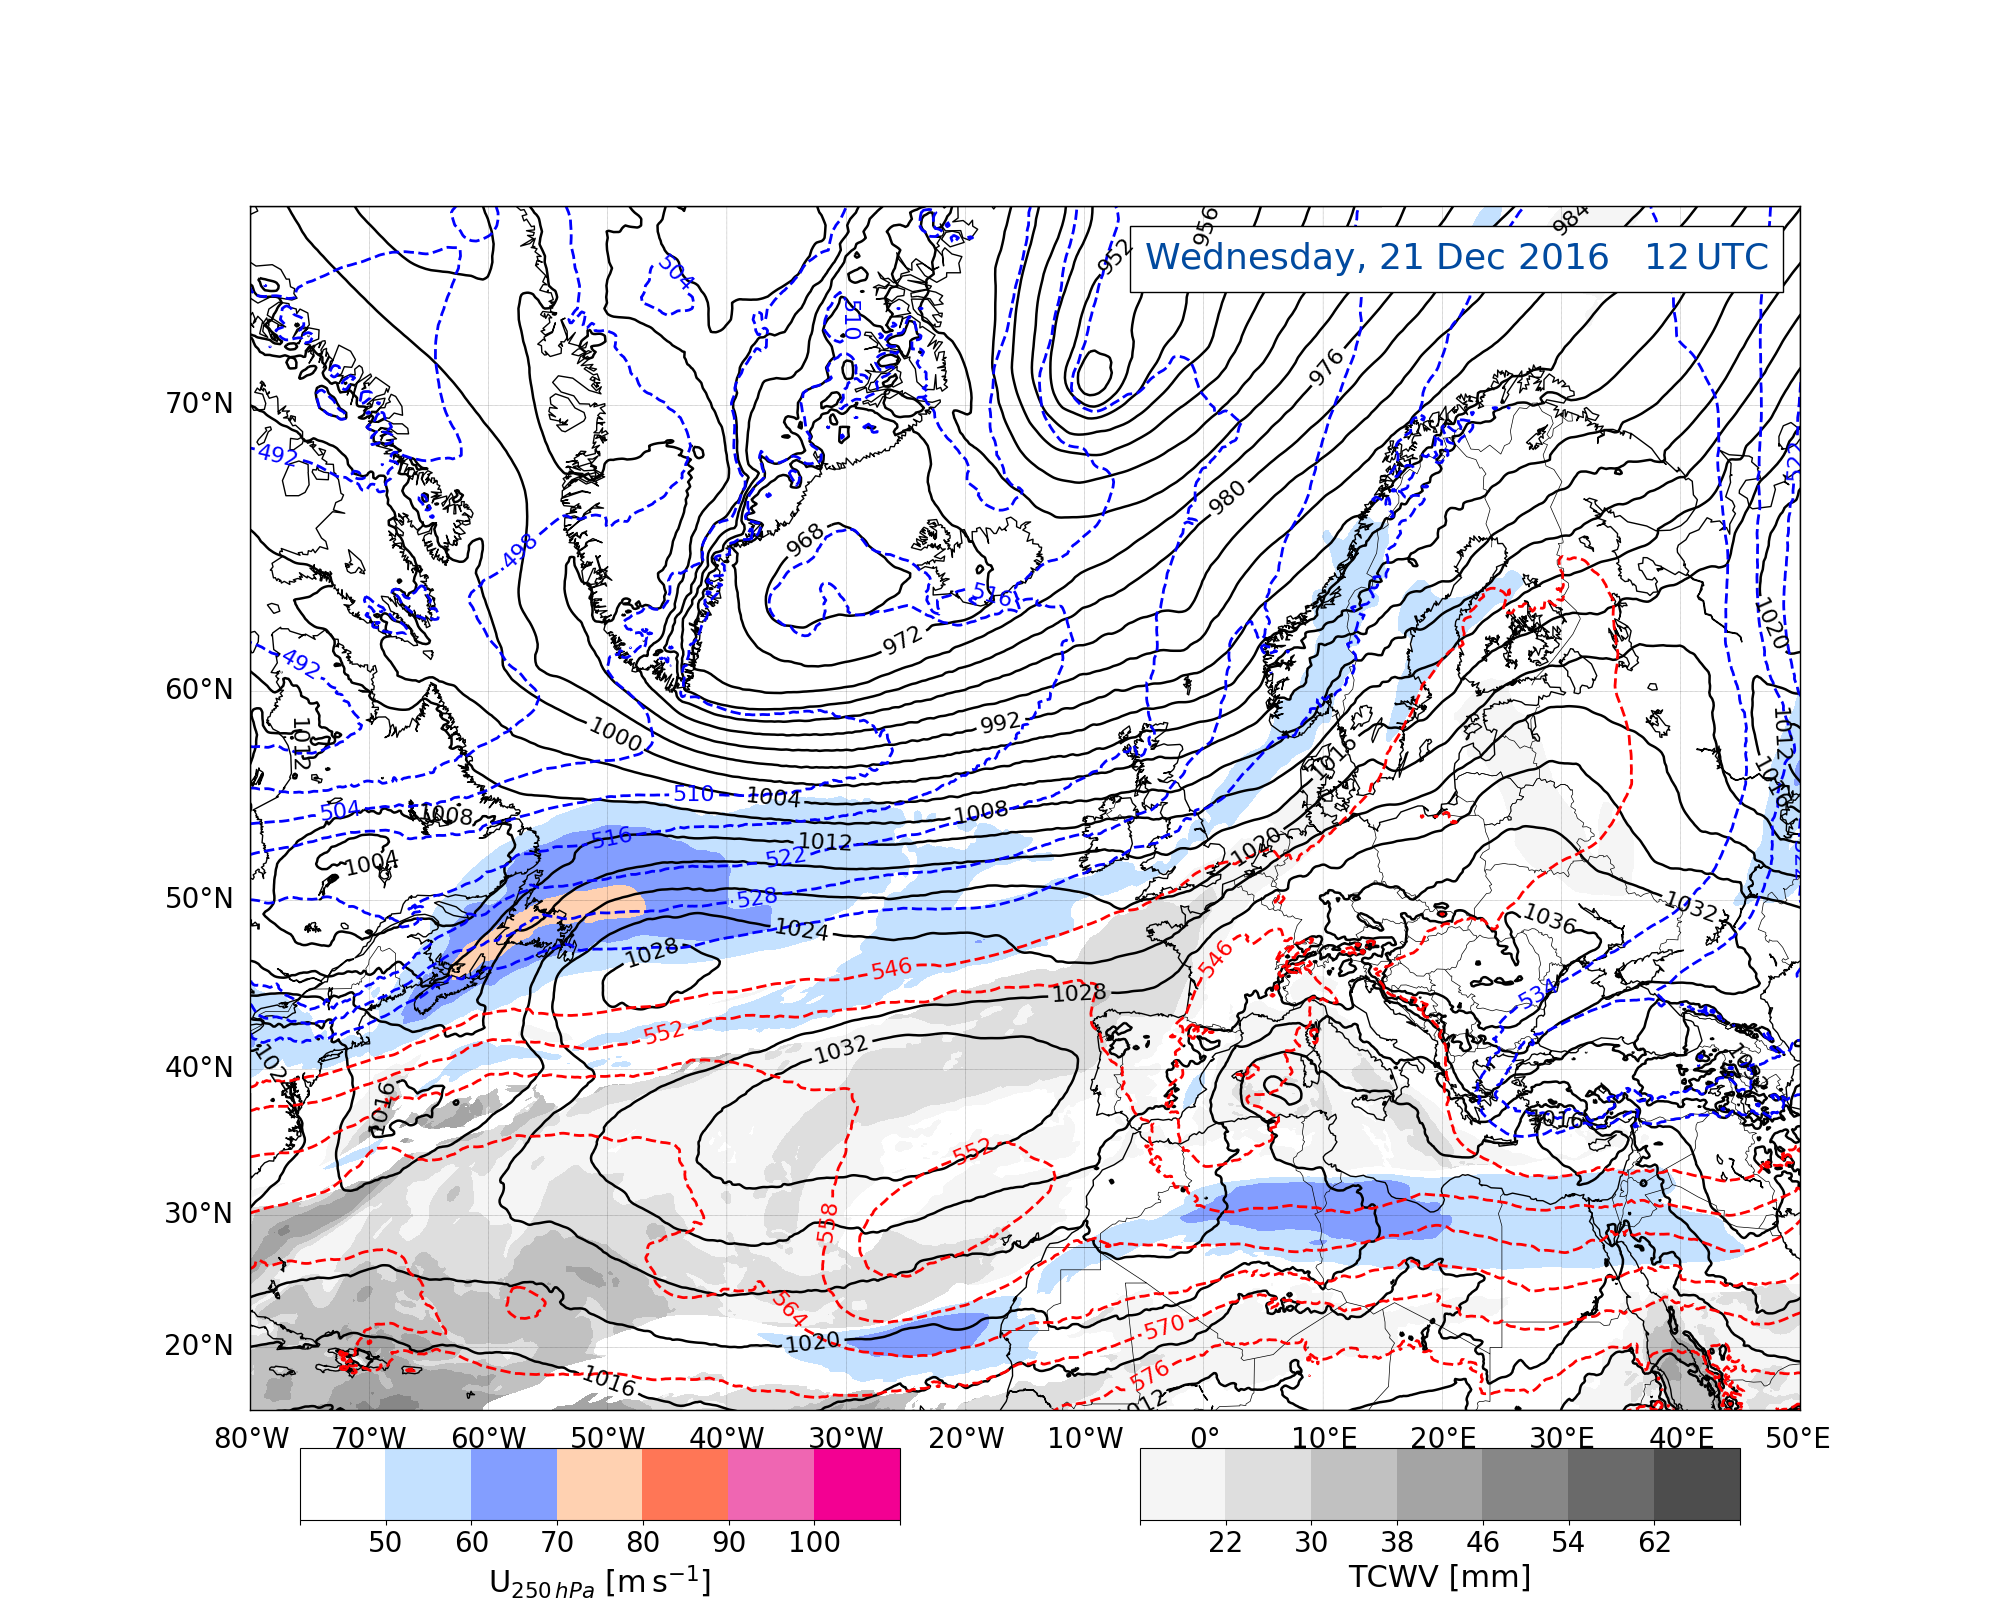
\includegraphics[trim={4.2cm 3.9cm 4.3cm 5.1cm},clip,
        width=\textwidth]{./fig_Geopot_Jet/20161221_12}
        \caption{}\label{fig:GP21}
    \end{subfigure}
%%%%%% 22/12
	\begin{subfigure}[b]{0.49\textwidth}
		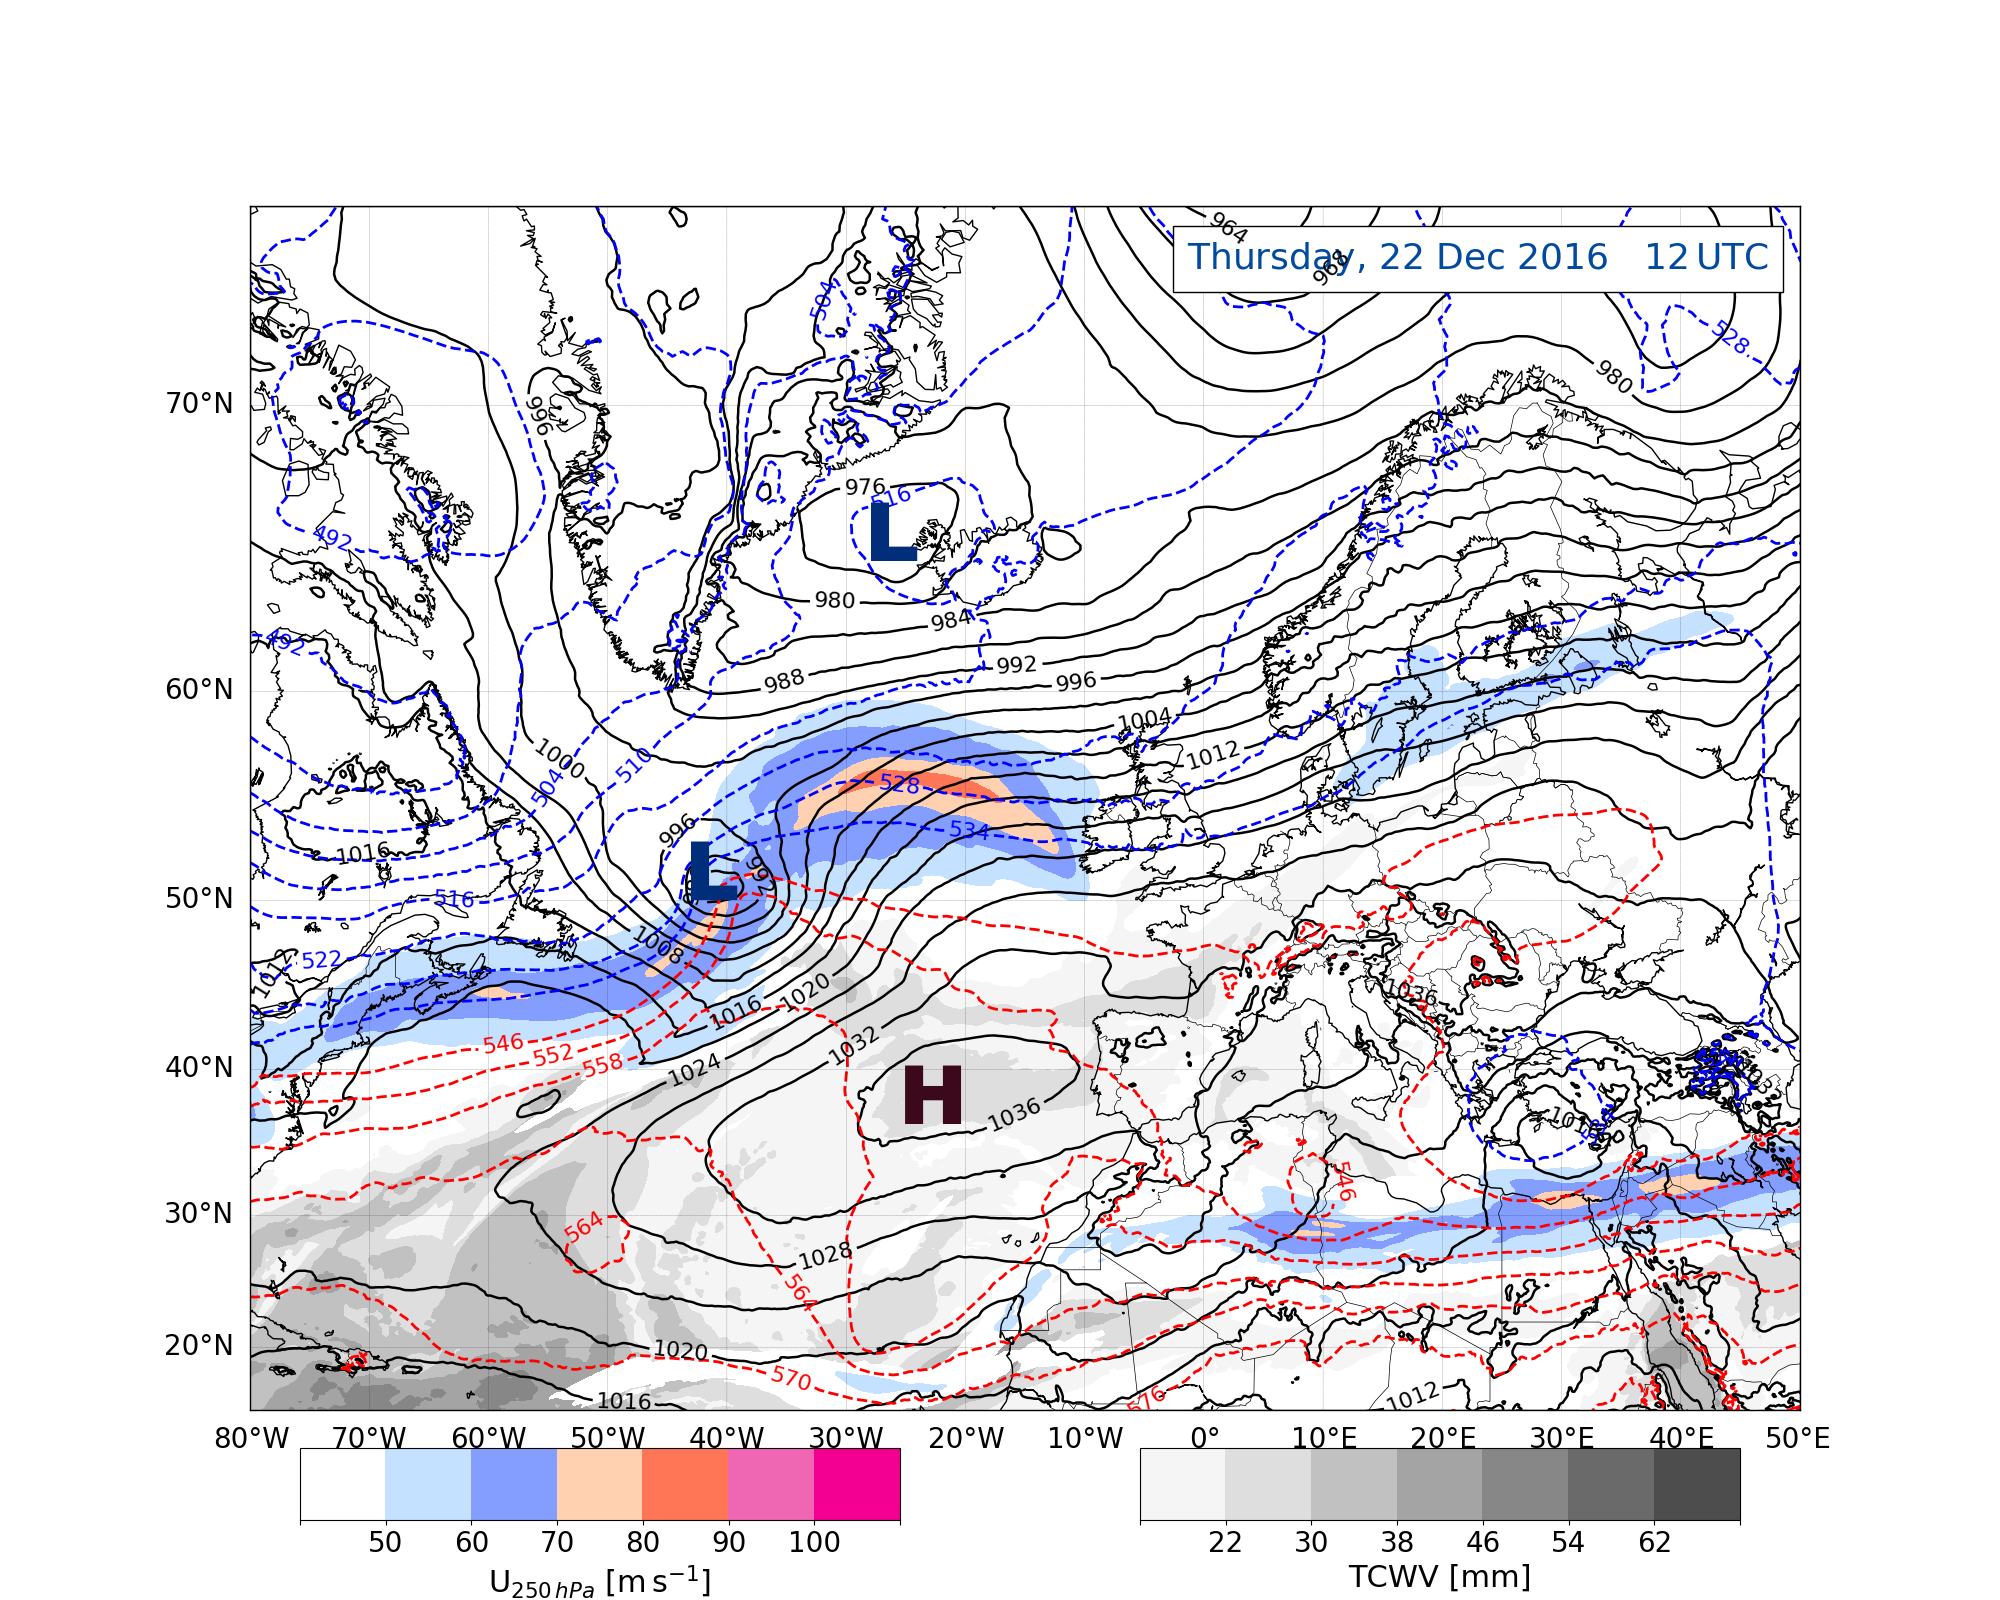
\includegraphics[trim={4.2cm 3.9cm 4.3cm 5.1cm},clip,
	width=\textwidth]{./fig_Geopot_Jet/20161222_12}
		\caption{}\label{fig:GP22}
	%\label{fig:sfc2100}
	\end{subfigure}
%%%%%% 23/12
	\begin{subfigure}[b]{0.49\textwidth}
		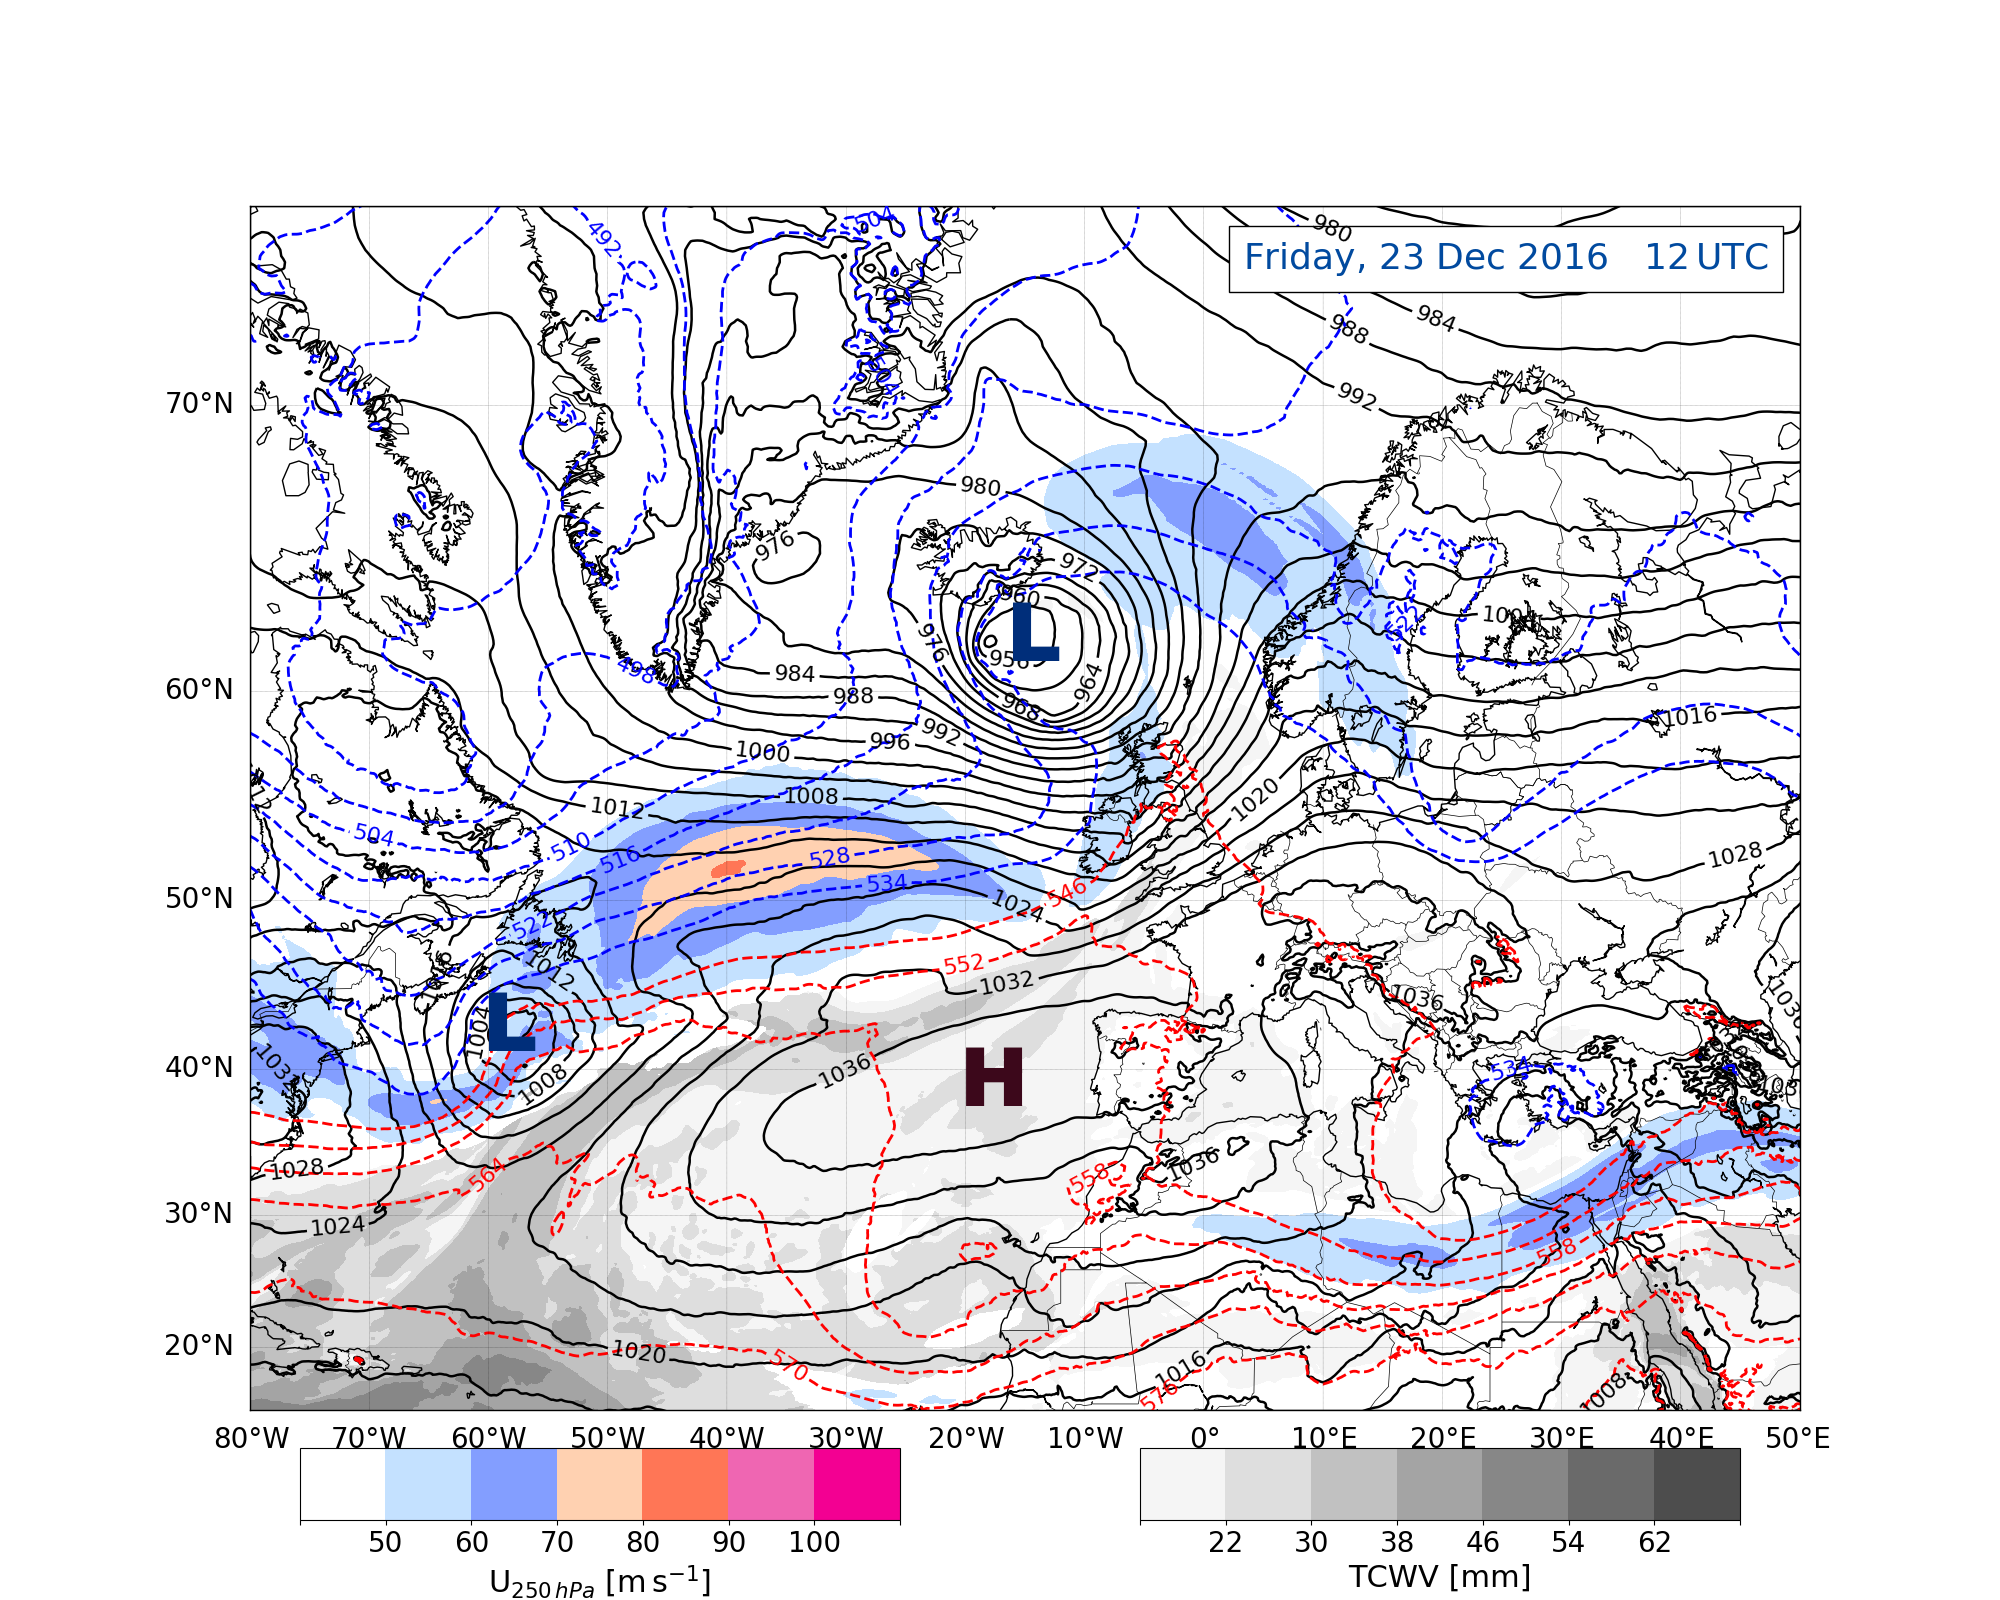
\includegraphics[trim={4.2cm 3.9cm 4.3cm 5.1cm},clip,
	width=\textwidth]{./fig_Geopot_Jet/20161223_12}
		\caption{}\label{fig:GP23}
	\end{subfigure}
%%%%%% label
    \begin{subfigure}[b]{\textwidth}
        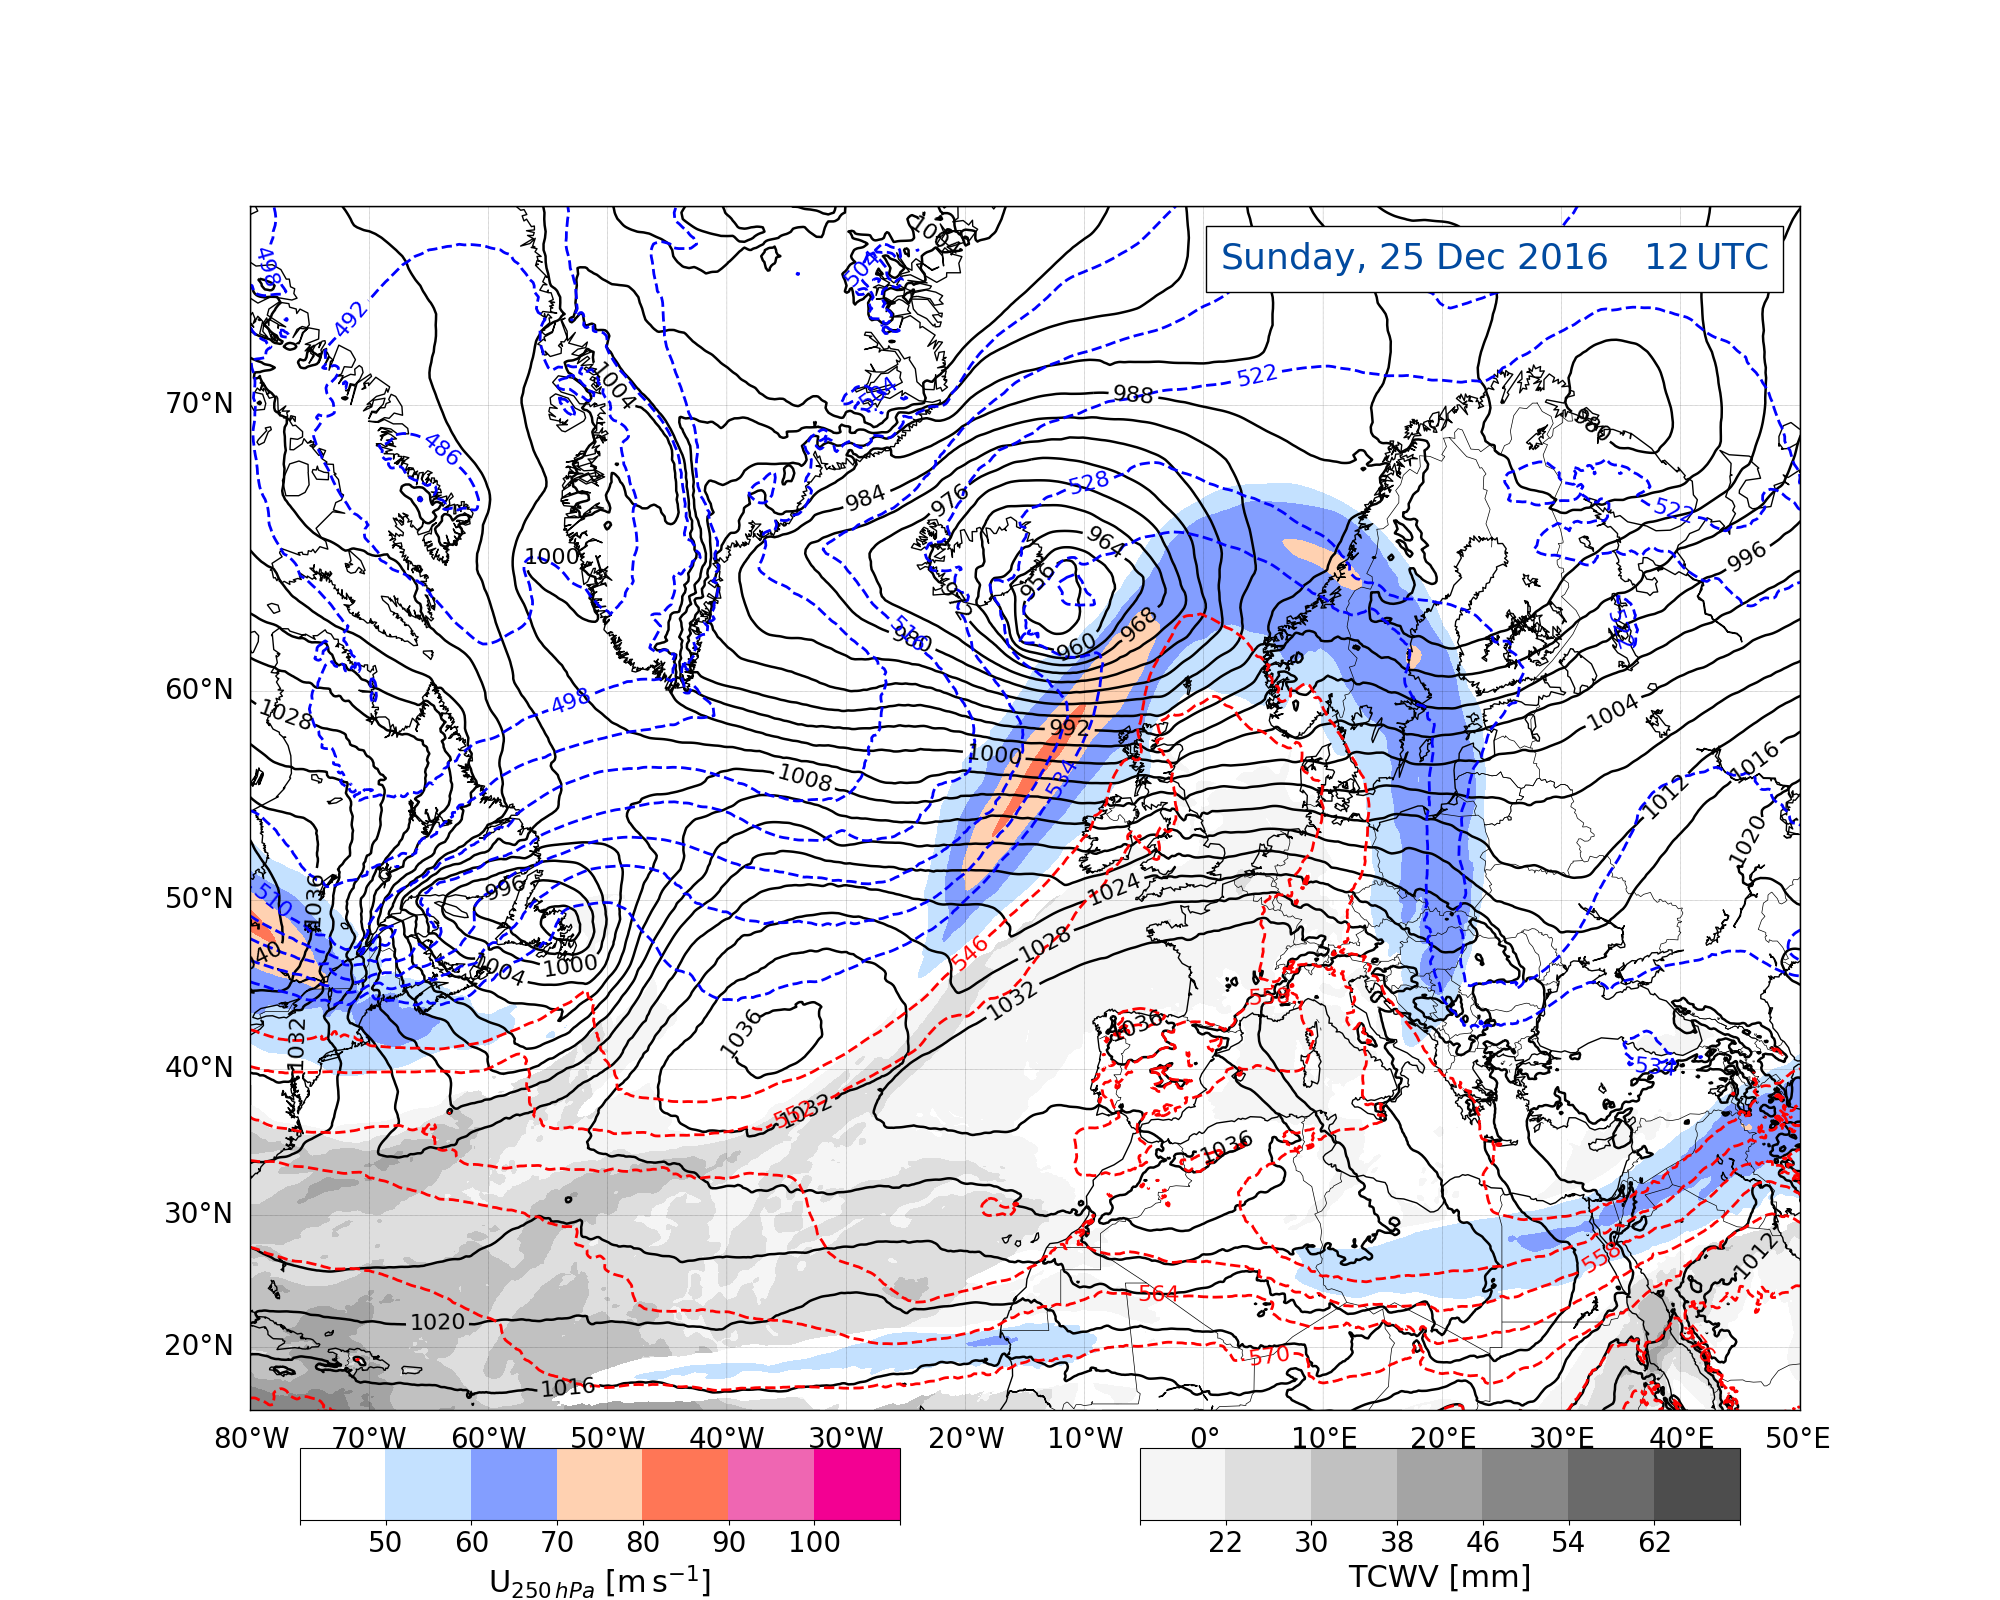
\includegraphics[trim={4.2cm 0cm 4.3cm 36.8cm},clip,
        width=\textwidth]{./fig_Geopot_Jet/20161225_12}
    \end{subfigure}
\caption{Jet, thickness, mean sea level pressure, and moisture synoptic analysis, data from ECMWF. During \SIrange{20}{27}{\dec}. \SI{250}{\hPa} wind speed, shaded according to the colour bar, [\SI{}{\mPs}]. \SI{1000}-\SI{500}{\hPa} thickness, dashed contours every \SI{6}{\deca\meter}, MSLP, black contours every \SI{4}{\hPa}, total column water vapour [\SI{}{\mm}], shaded according the grey scale.}\label{fig:GeopJet}
\end{figure}
\begin{figure}\ContinuedFloat
	\centering
%%%%%% 24/12
    \begin{subfigure}[b]{0.49\textwidth}
        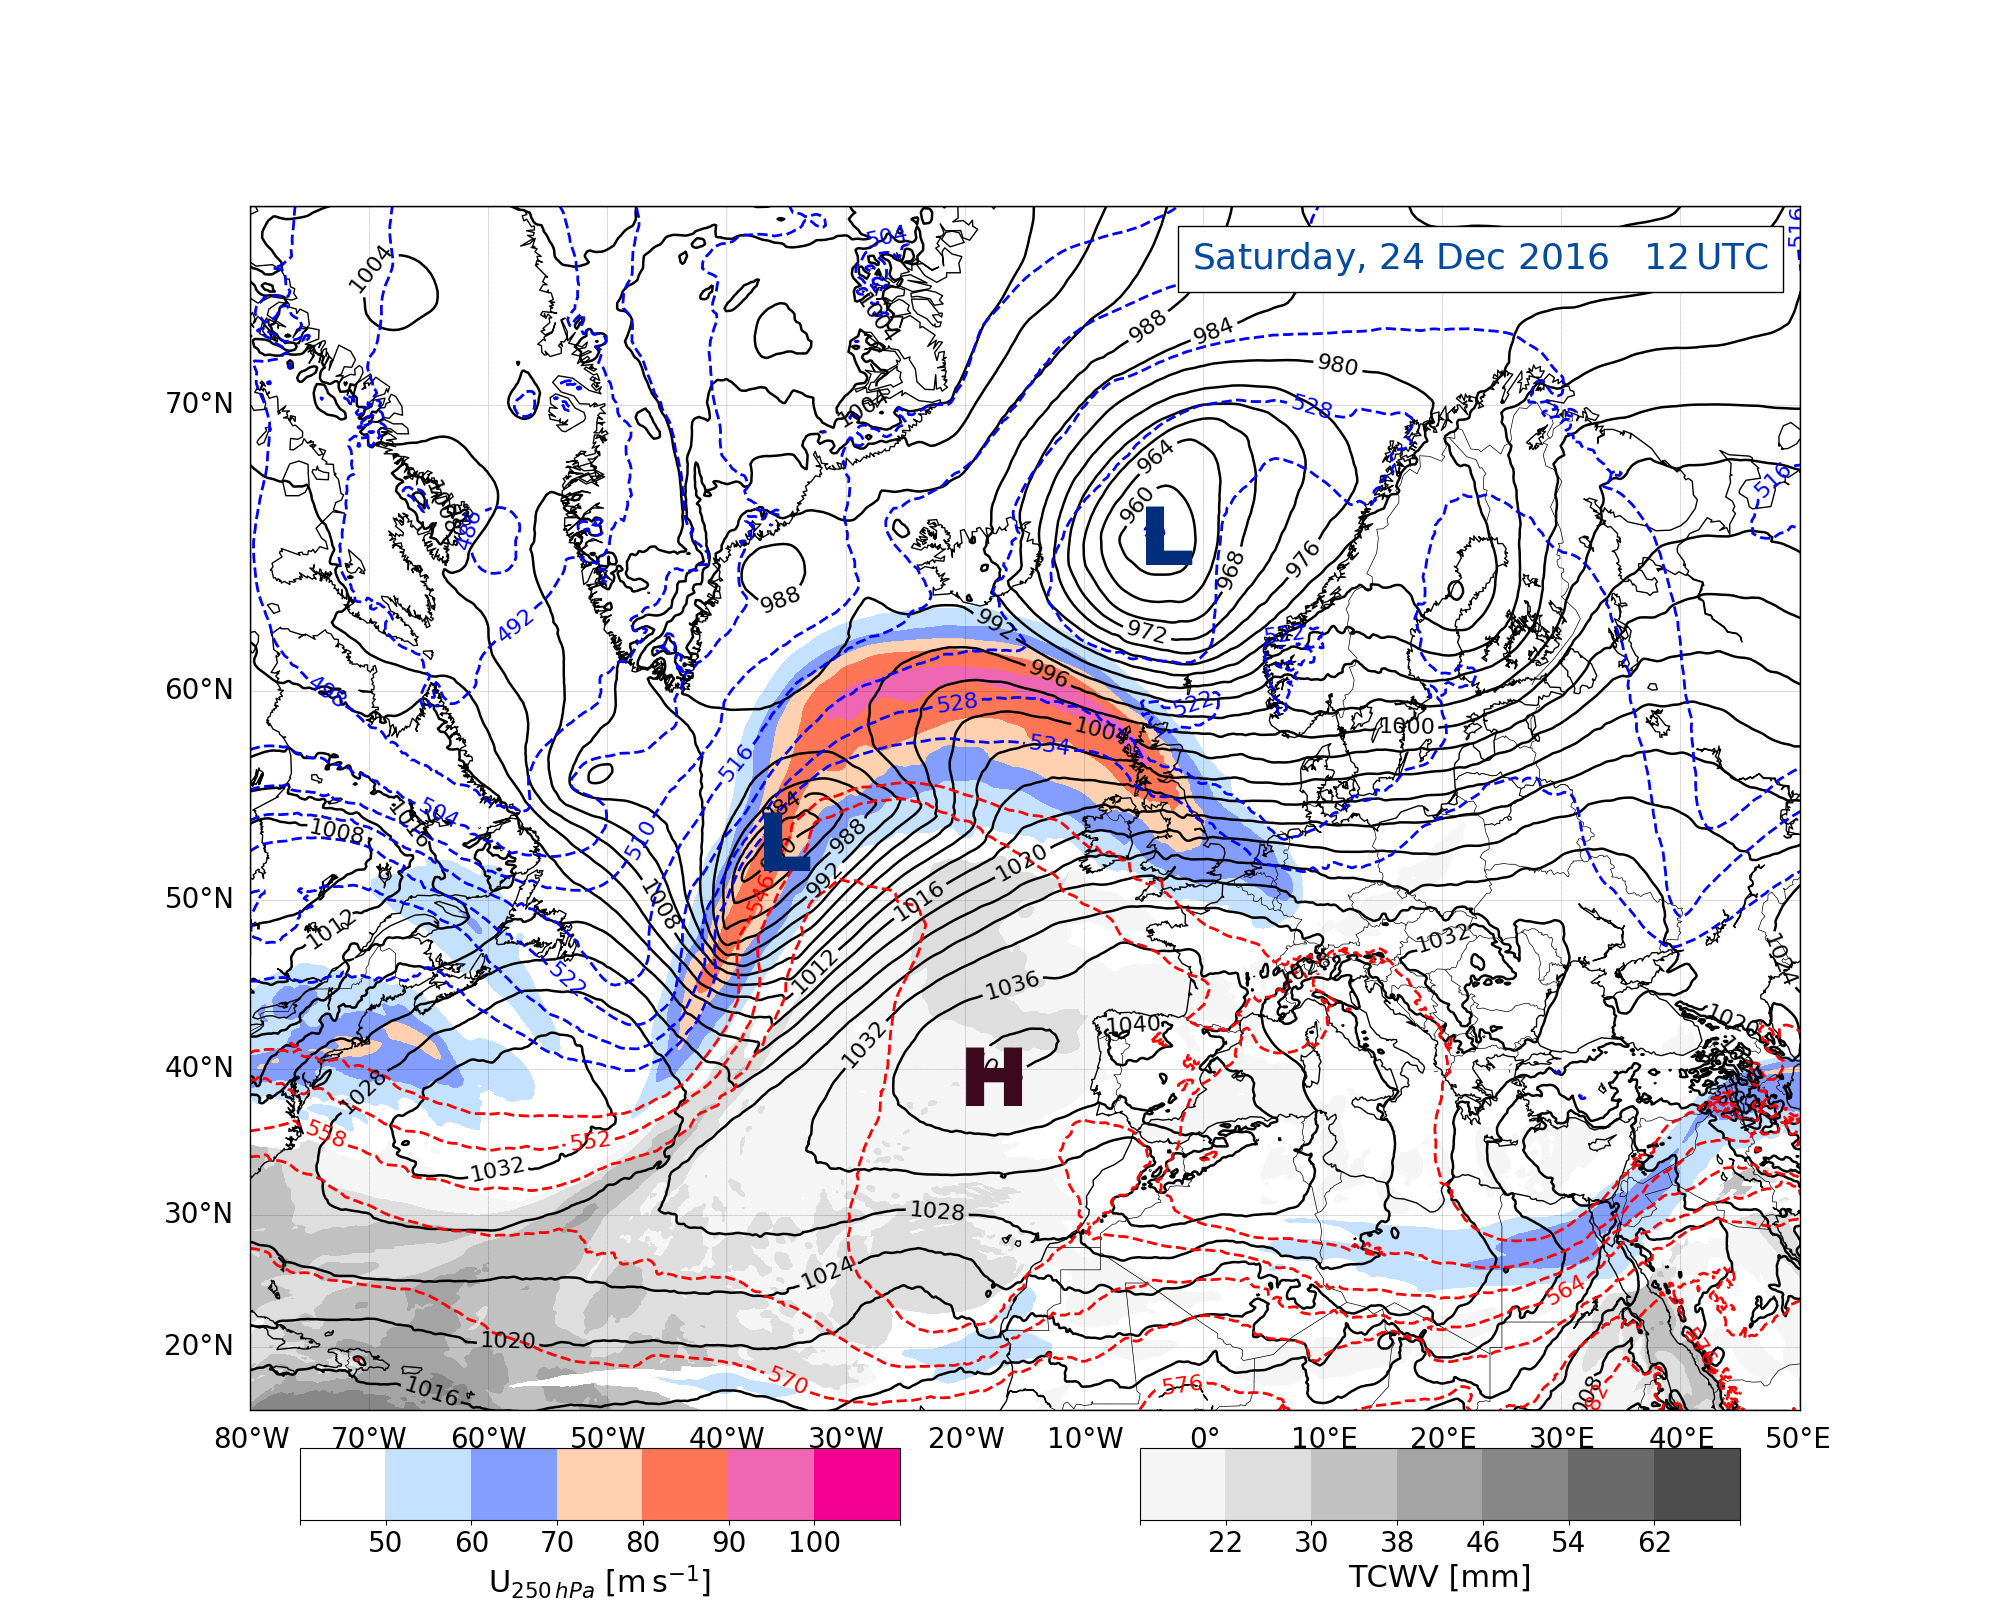
\includegraphics[trim={4.2cm 3.9cm 4.3cm 5.1cm},clip,
        width=\textwidth]{./fig_Geopot_Jet/20161224_12}
        \caption{}\label{fig:GP24}
    \end{subfigure}
%%%%%% 25/12
    \begin{subfigure}[b]{0.49\textwidth}
        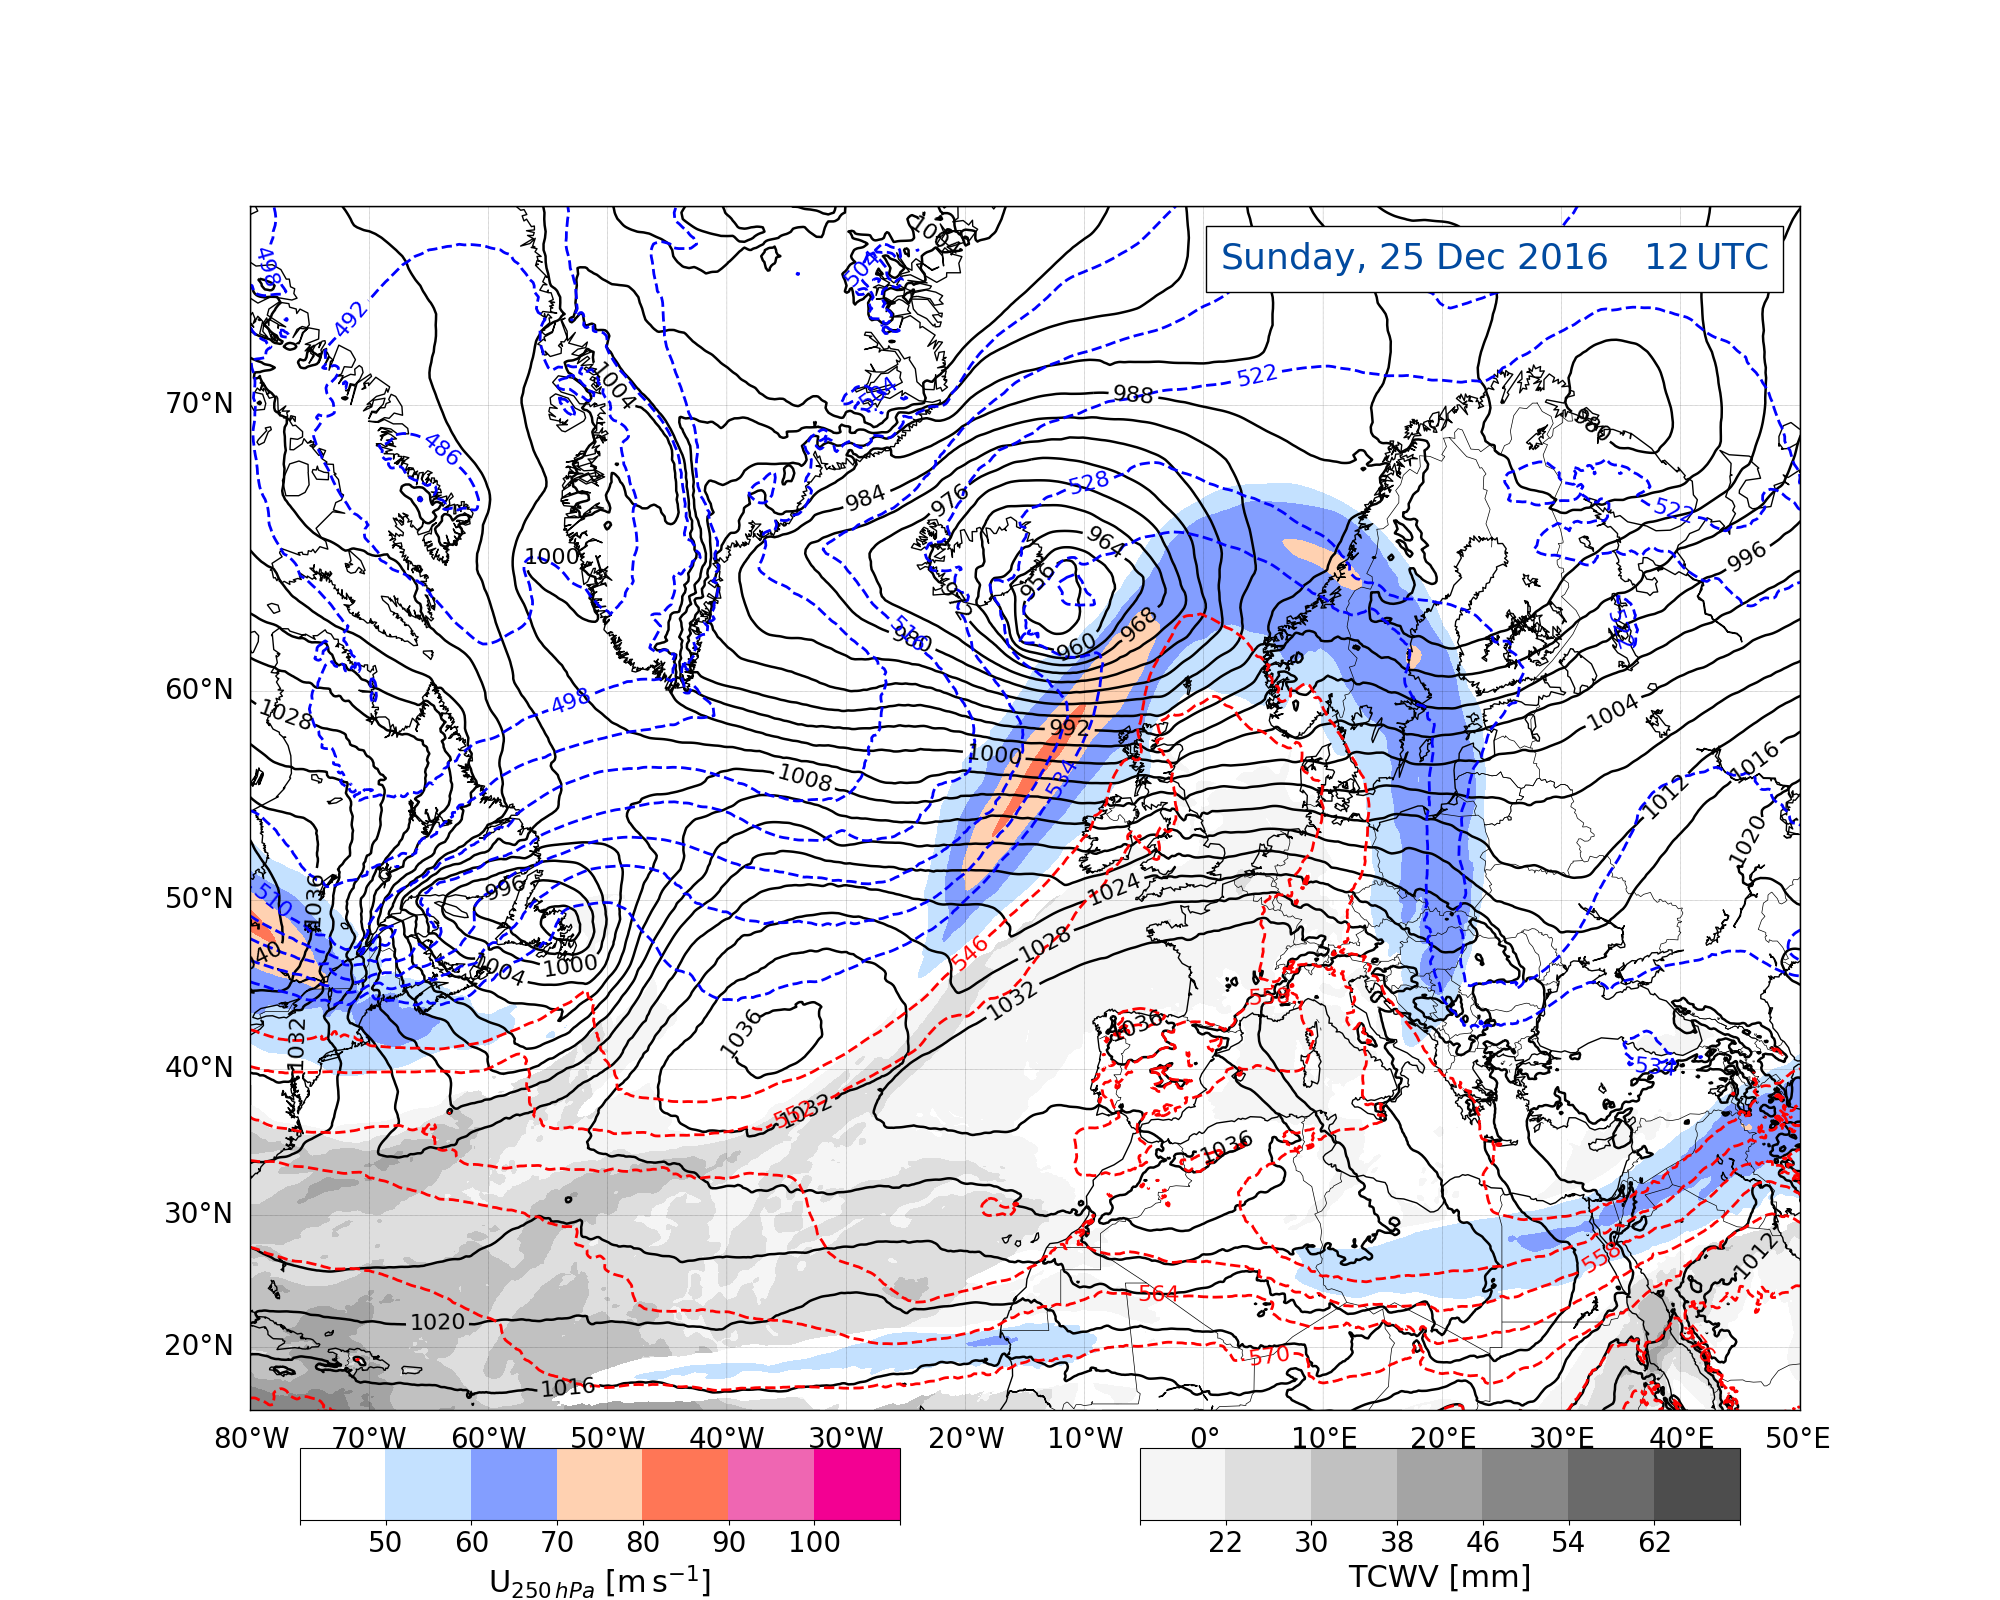
\includegraphics[trim={4.2cm 3.9cm 4.3cm 5.1cm},clip,
        width=\textwidth]{./fig_Geopot_Jet/20161225_12}
        \caption{}\label{fig:GP25}
    \end{subfigure}
%	\centering
%%%%%% 26/12
    \begin{subfigure}[b]{0.49\textwidth}
        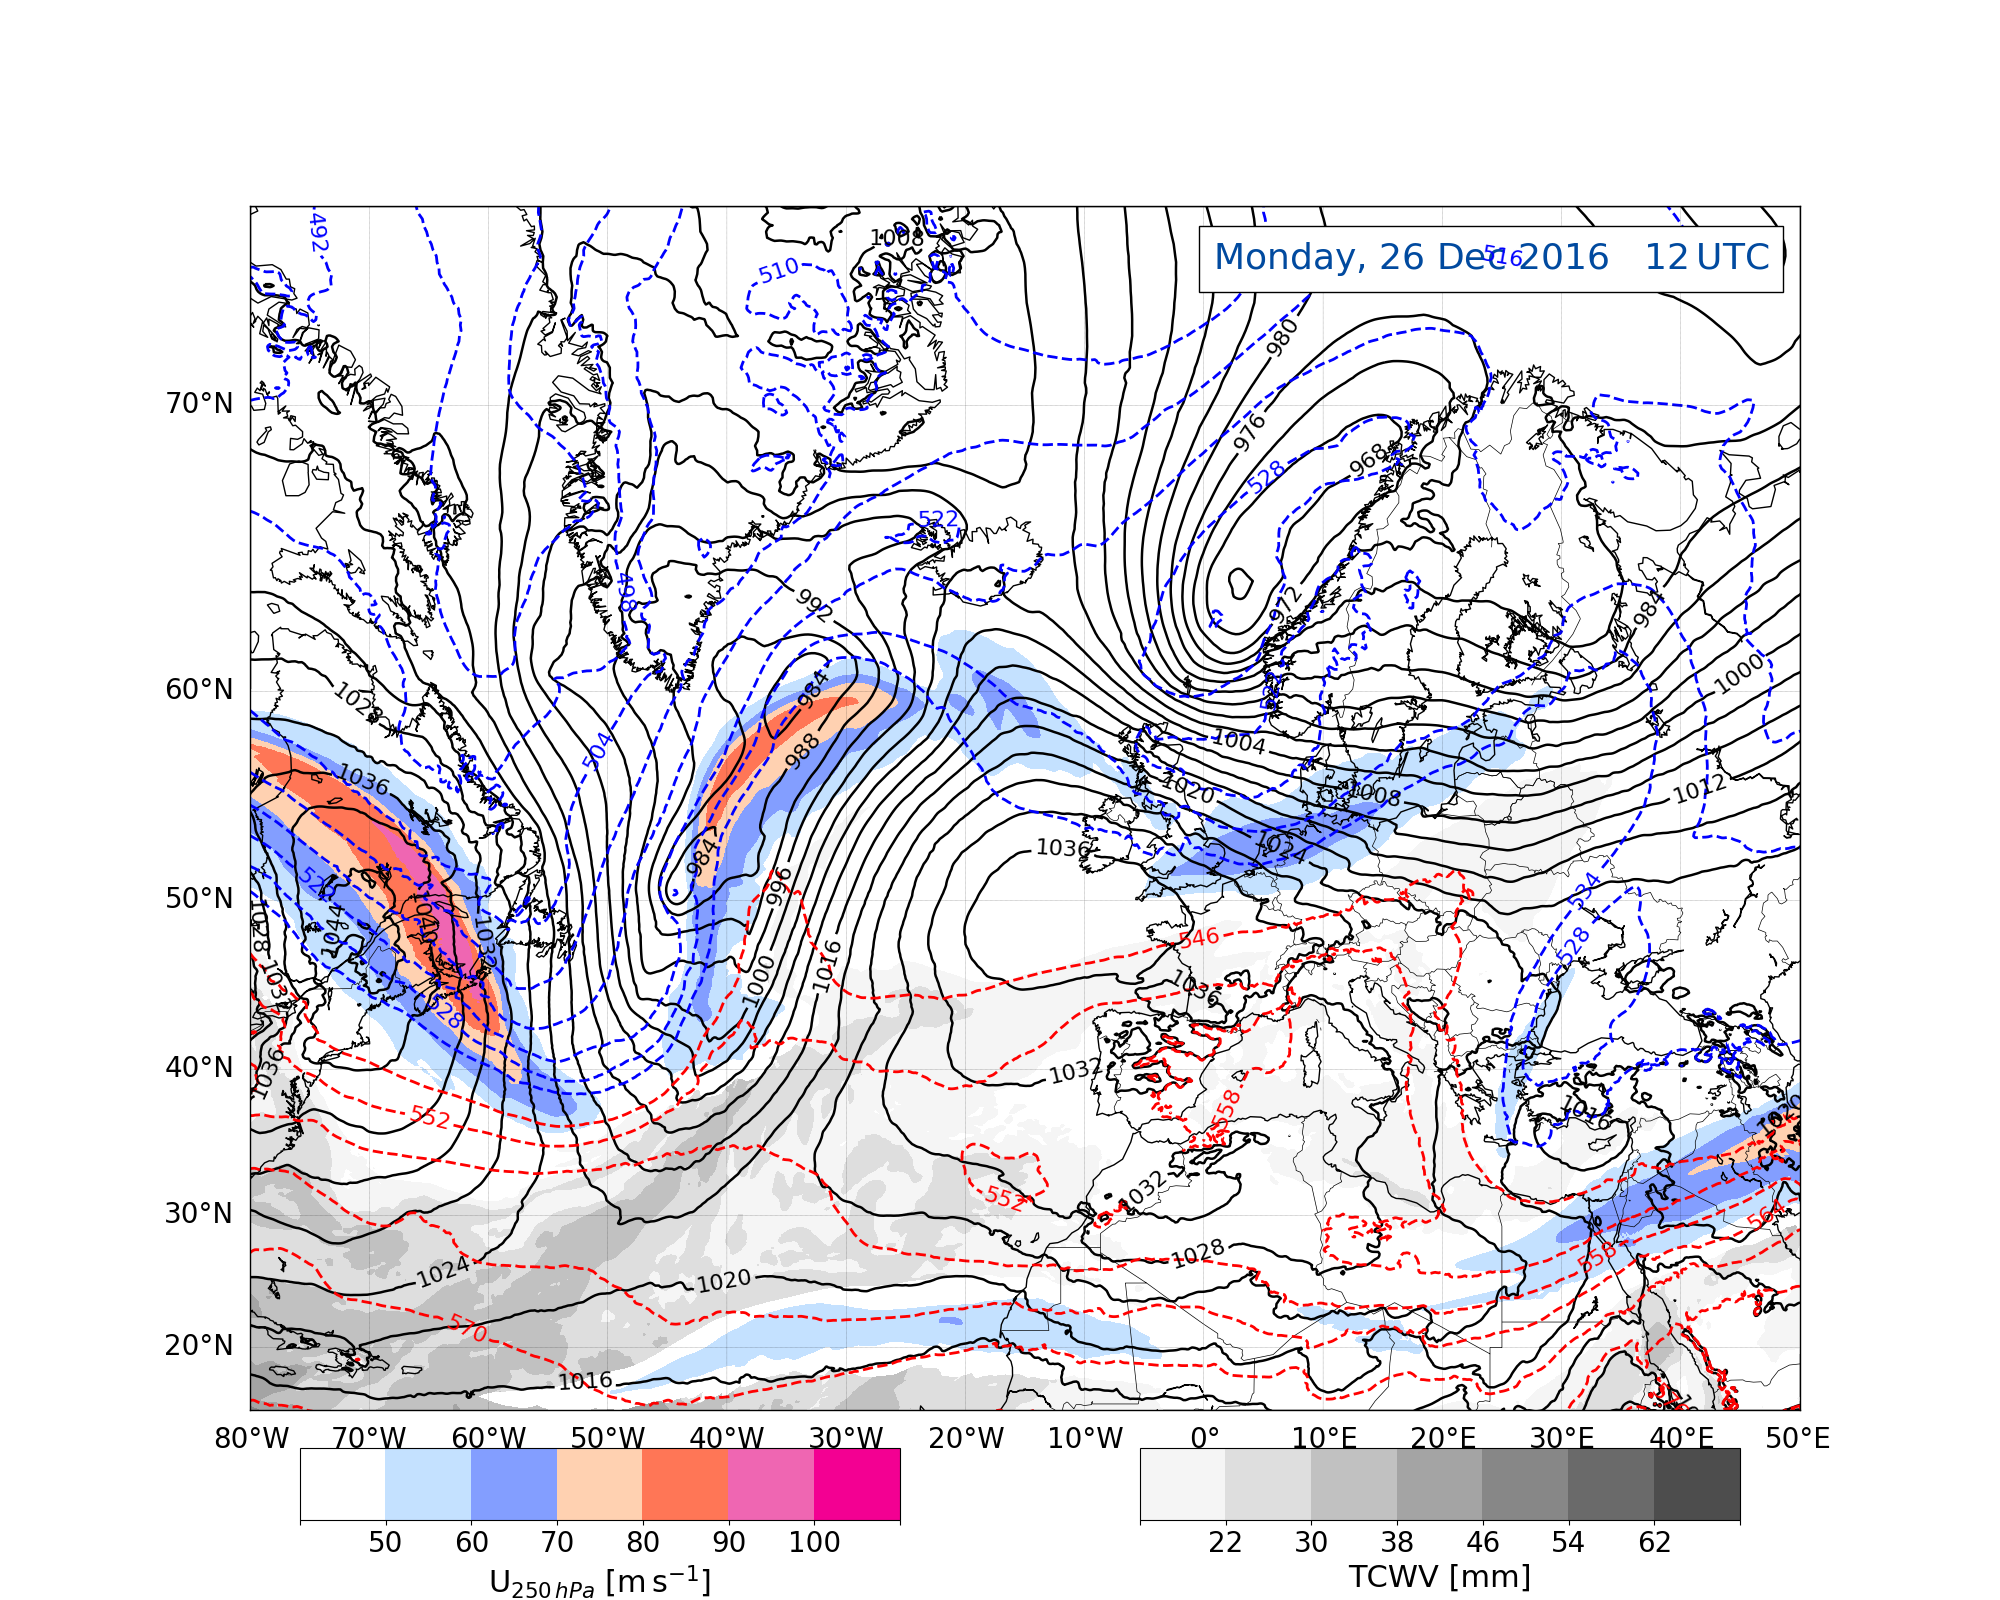
\includegraphics[trim={4.2cm 3.9cm 4.3cm 5.1cm},clip,
        width=\textwidth]{./fig_Geopot_Jet/20161226_12}
        \caption{}\label{fig:GP26}
    \end{subfigure}
%%%%%% 27/12
    \begin{subfigure}[b]{0.49\textwidth}
        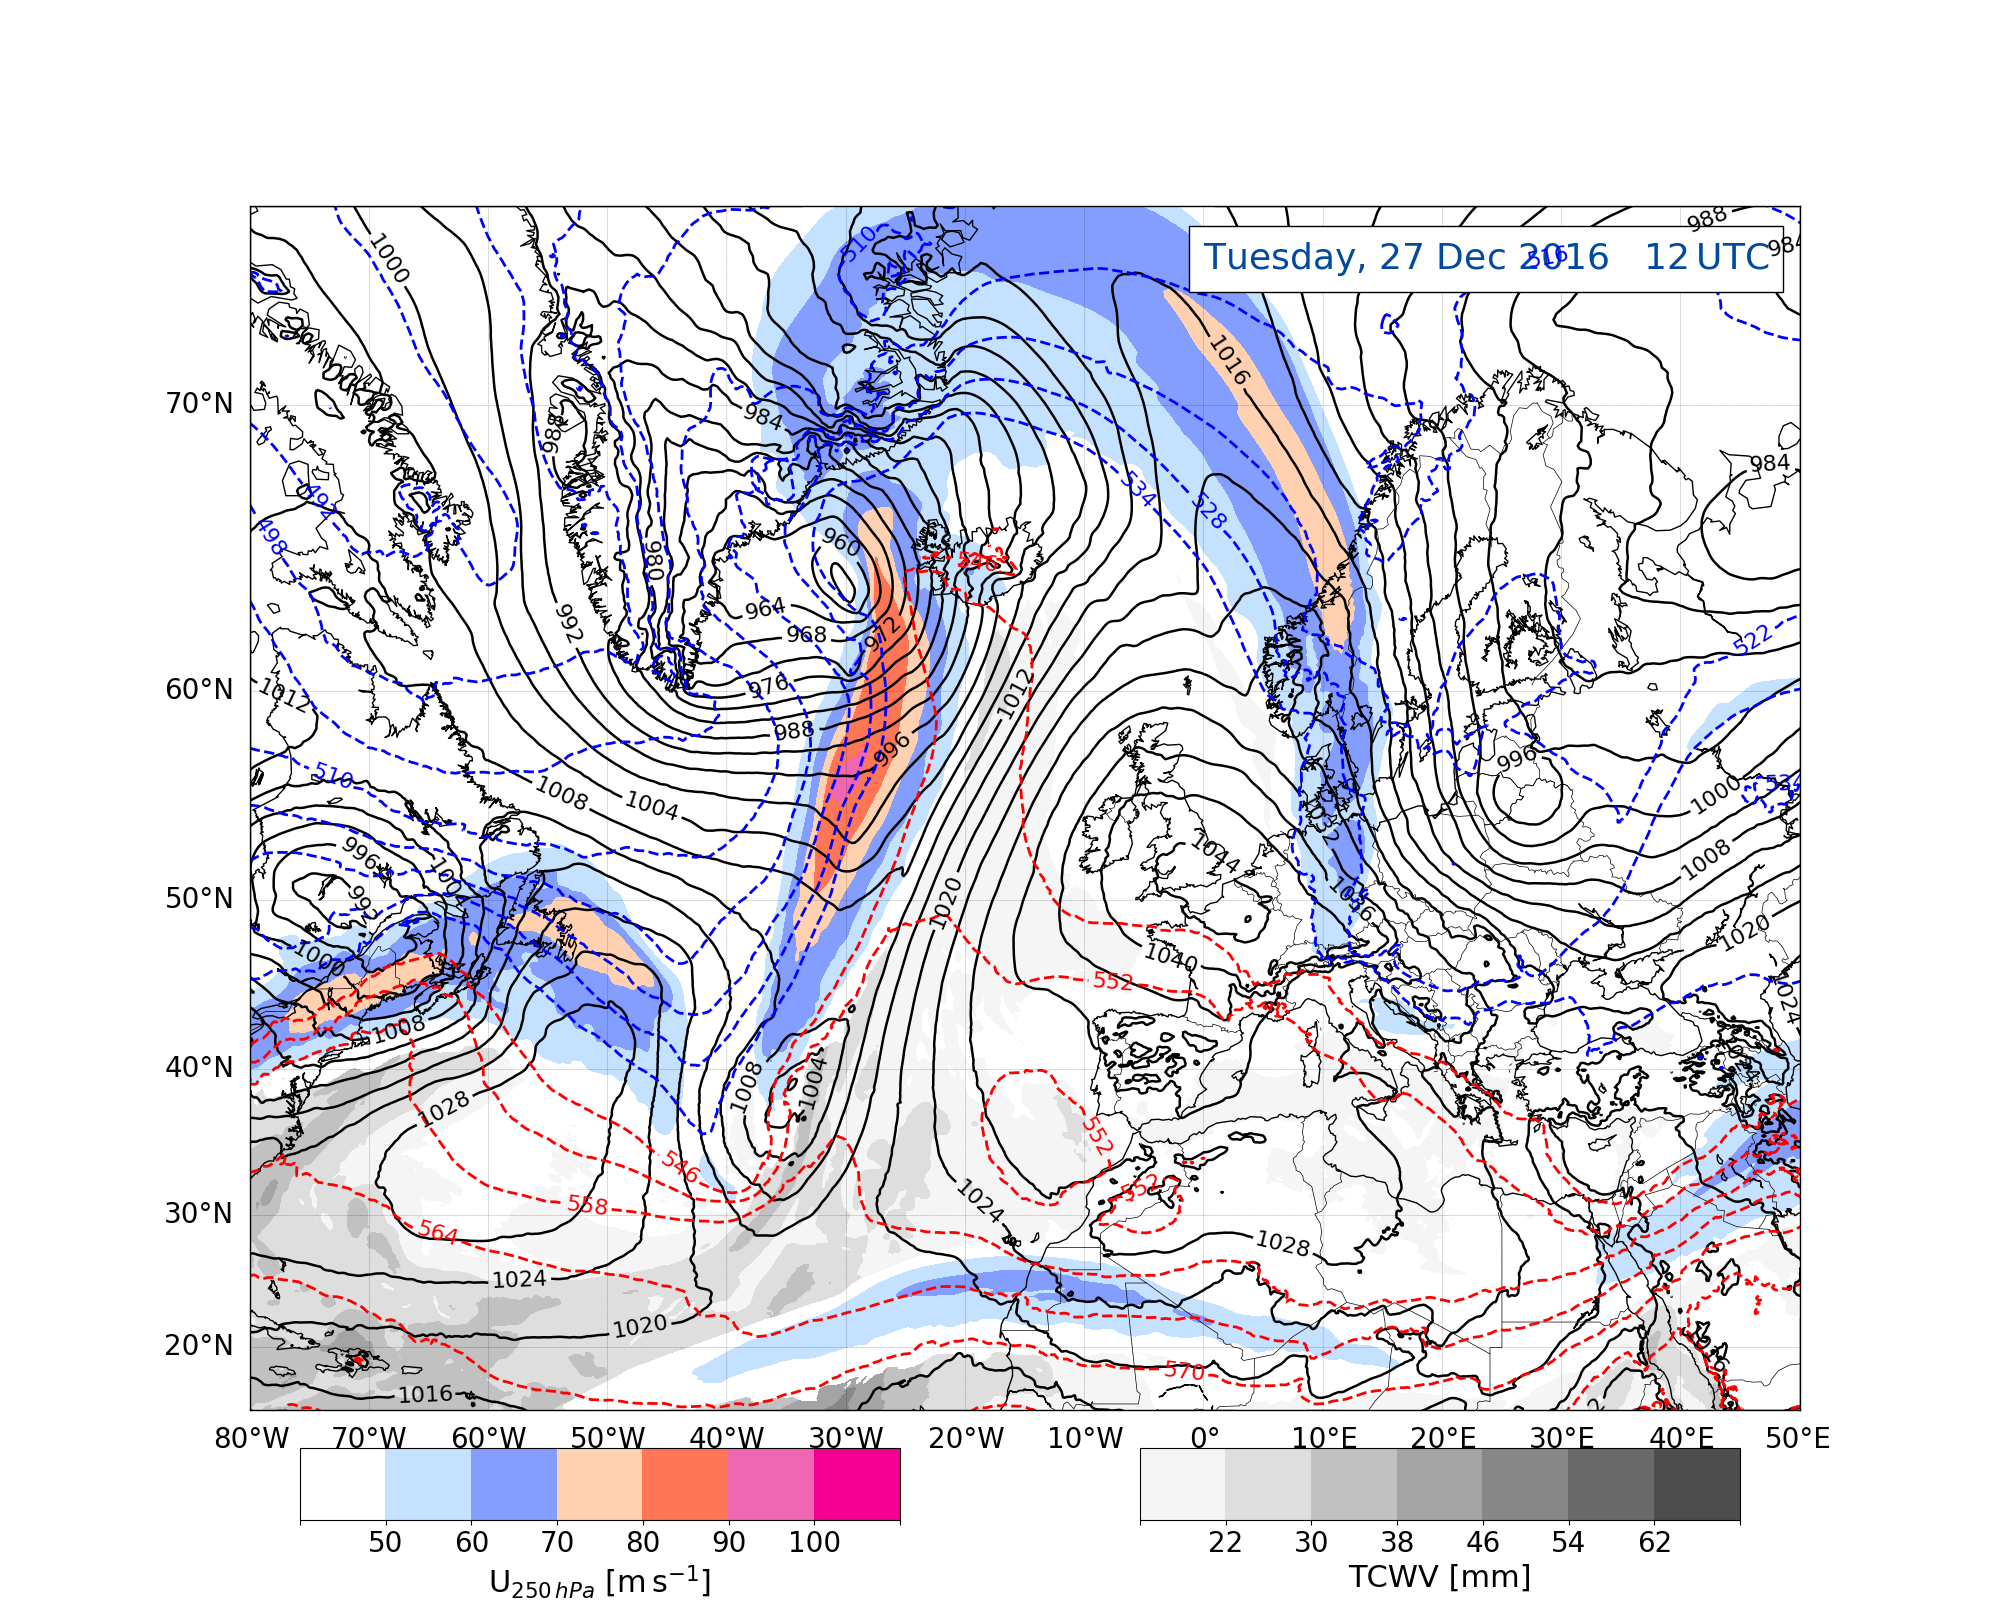
\includegraphics[trim={4.2cm 3.9cm 4.3cm 5.1cm},clip,
        width=\textwidth]{./fig_Geopot_Jet/20161227_12}
        \caption{}\label{fig:GP27}
    \end{subfigure}
%%%%%% label
    \begin{subfigure}[b]{\textwidth}
        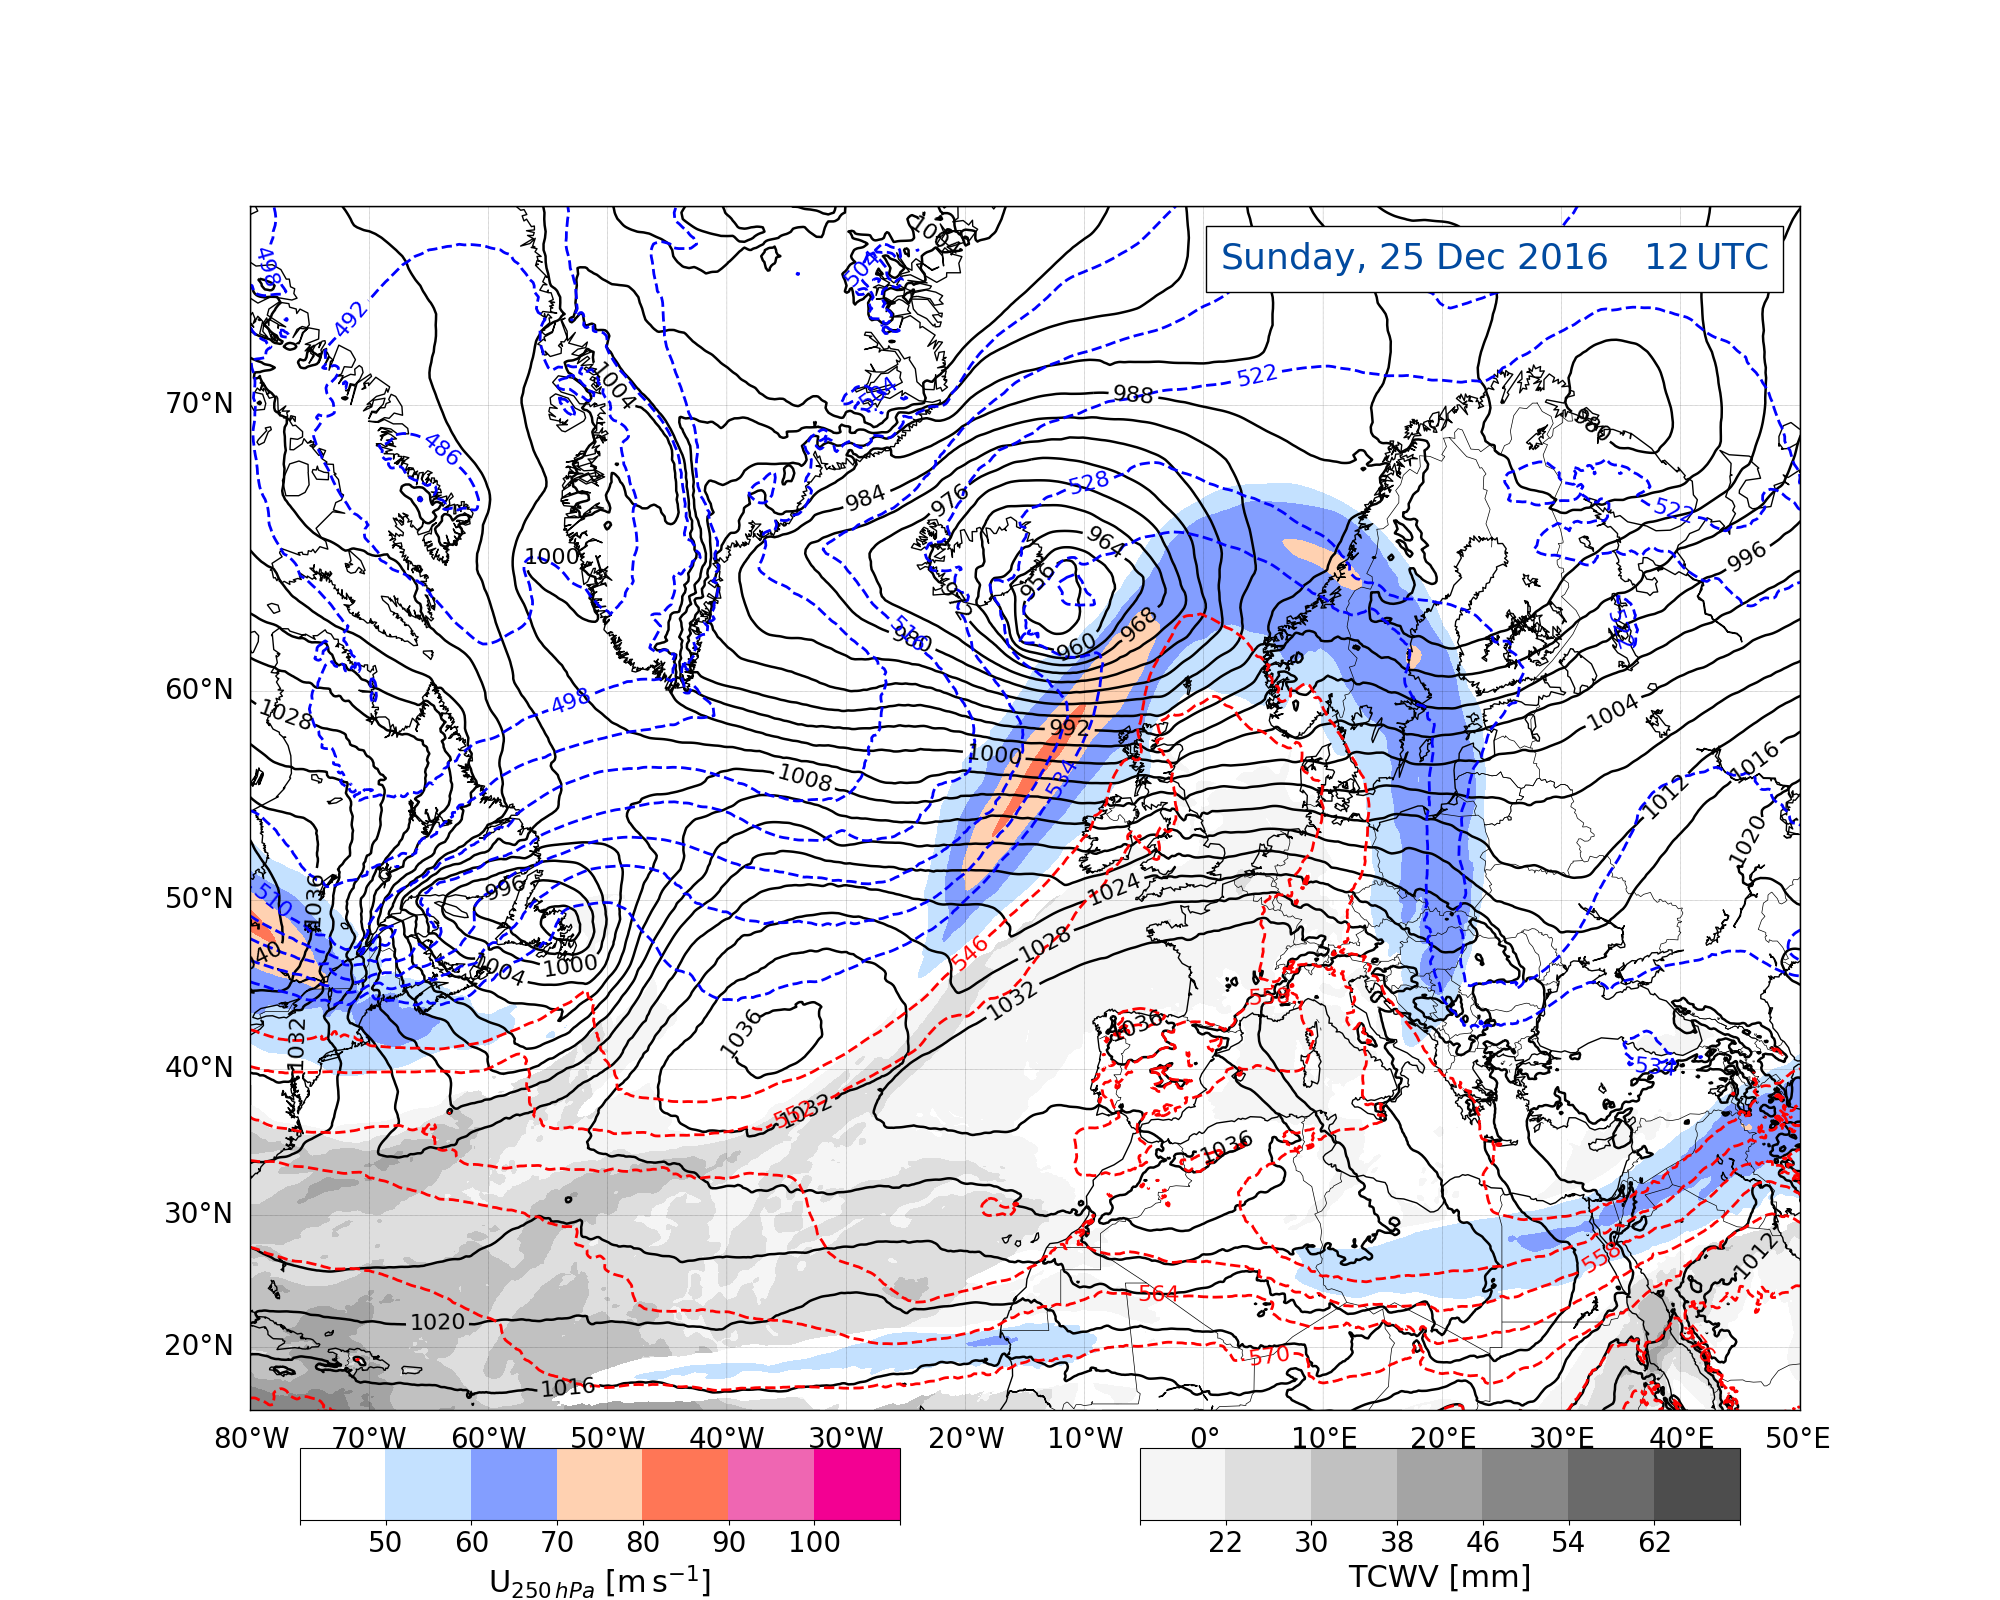
\includegraphics[trim={4.2cm 0cm 4.3cm 36.8cm},clip,
        width=\textwidth]{./fig_Geopot_Jet/20161225_12}
       % \label{fig:D}
    \end{subfigure}
\caption{\textit{(Continued from previous page.)}}   
\end{figure}
% %%%%%%%%%%%%%%%%%%%%%%%%%%%%%%%%%%%%%%%%%%%%%%%%%%%%%%%%%%%%%%%%%%%%%%%%%
\newpage
%% Presentation map %%%%%%%%%%%%%%%%%%%%%%%%%%%%%%%%%%%%%
% !TeX spellcheck = en_GB
%%%%%% 20/12 DT
\noindent\begin{minipage}%[t][0.55\textheight]
[t]{.59\textwidth}
  	\centering
  		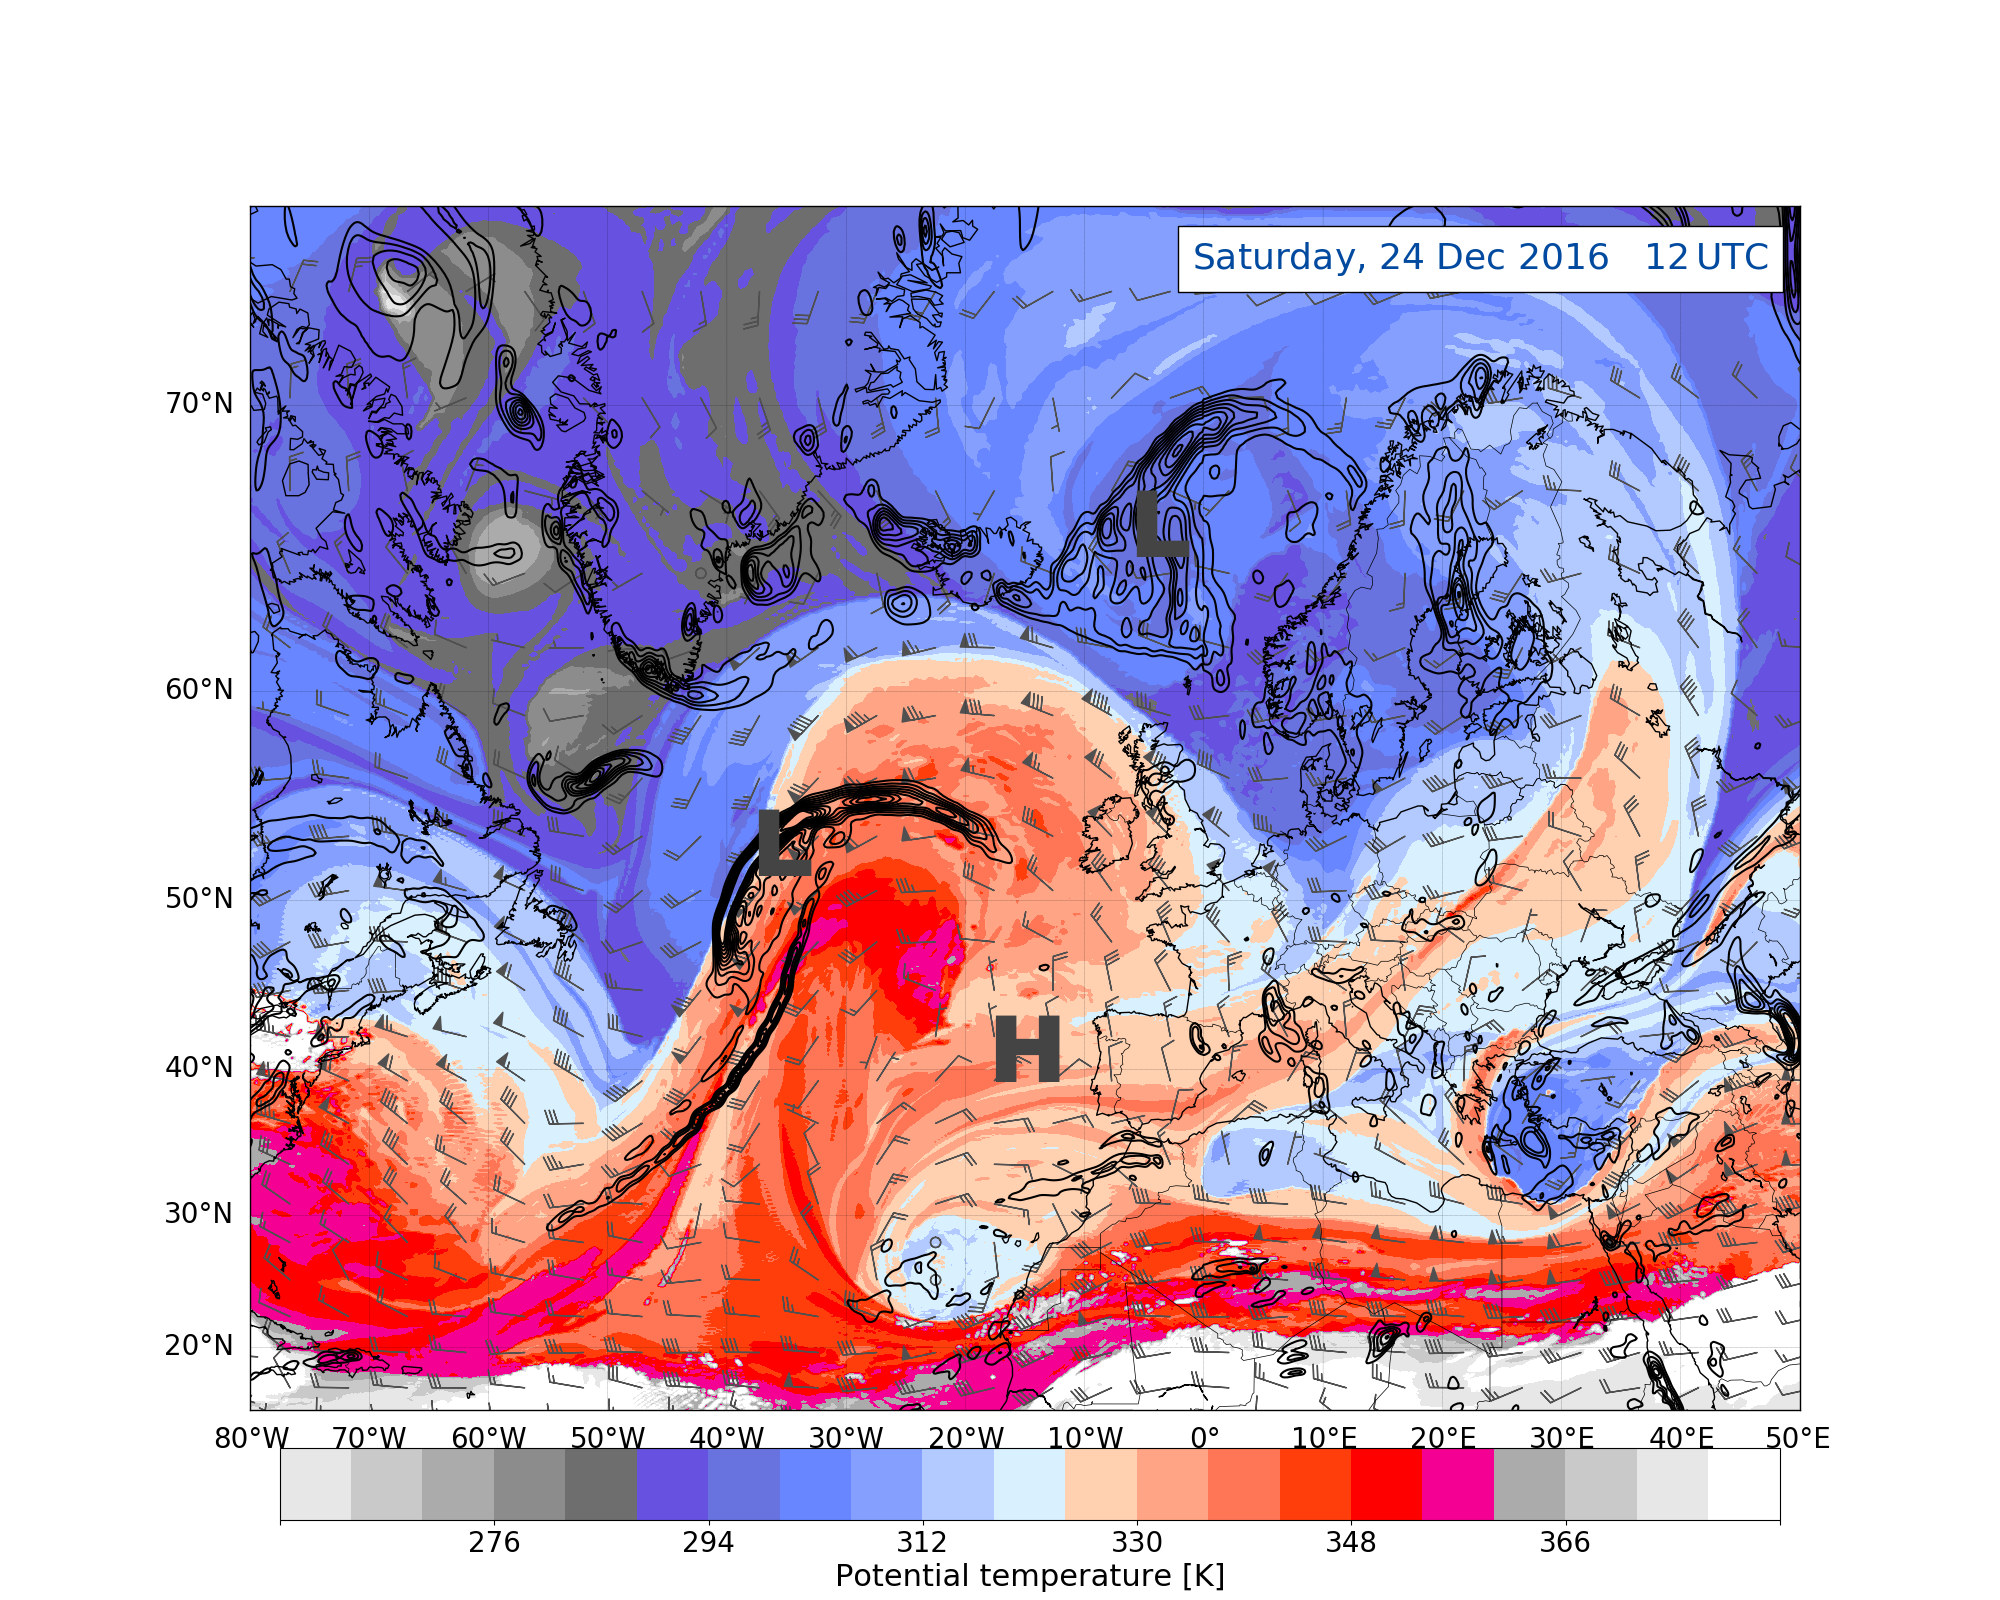
\includegraphics[trim={4.2cm 0cm 4.3cm 5.1cm},clip,
        width=\textwidth]{./fig_DynTropo/20161224_12_pres}
\end{minipage}\hfill
\begin{minipage}[b]{.4\textwidth}
	\captionof{subfigure}{Dynamic tropopause analysis map at \SI{2}{PVU}. Potential temperature [K] at the \SI{2}{PVU} surface, shaded according to the colour bar. Total wind, barbs [\SI{}{\mPs}], and \SI{925}--\SI{850}{\hPa} layer-averaged surface relative vorticity (black contours, every \SI{.5e-4}{\per\second}).} \label{fig:DT24_pres}
\end{minipage}
%%%%%% 20/12 slp thickness
\noindent\begin{minipage}%[t][0.55\textheight]
[t]{.59\textwidth}
  	\centering
  		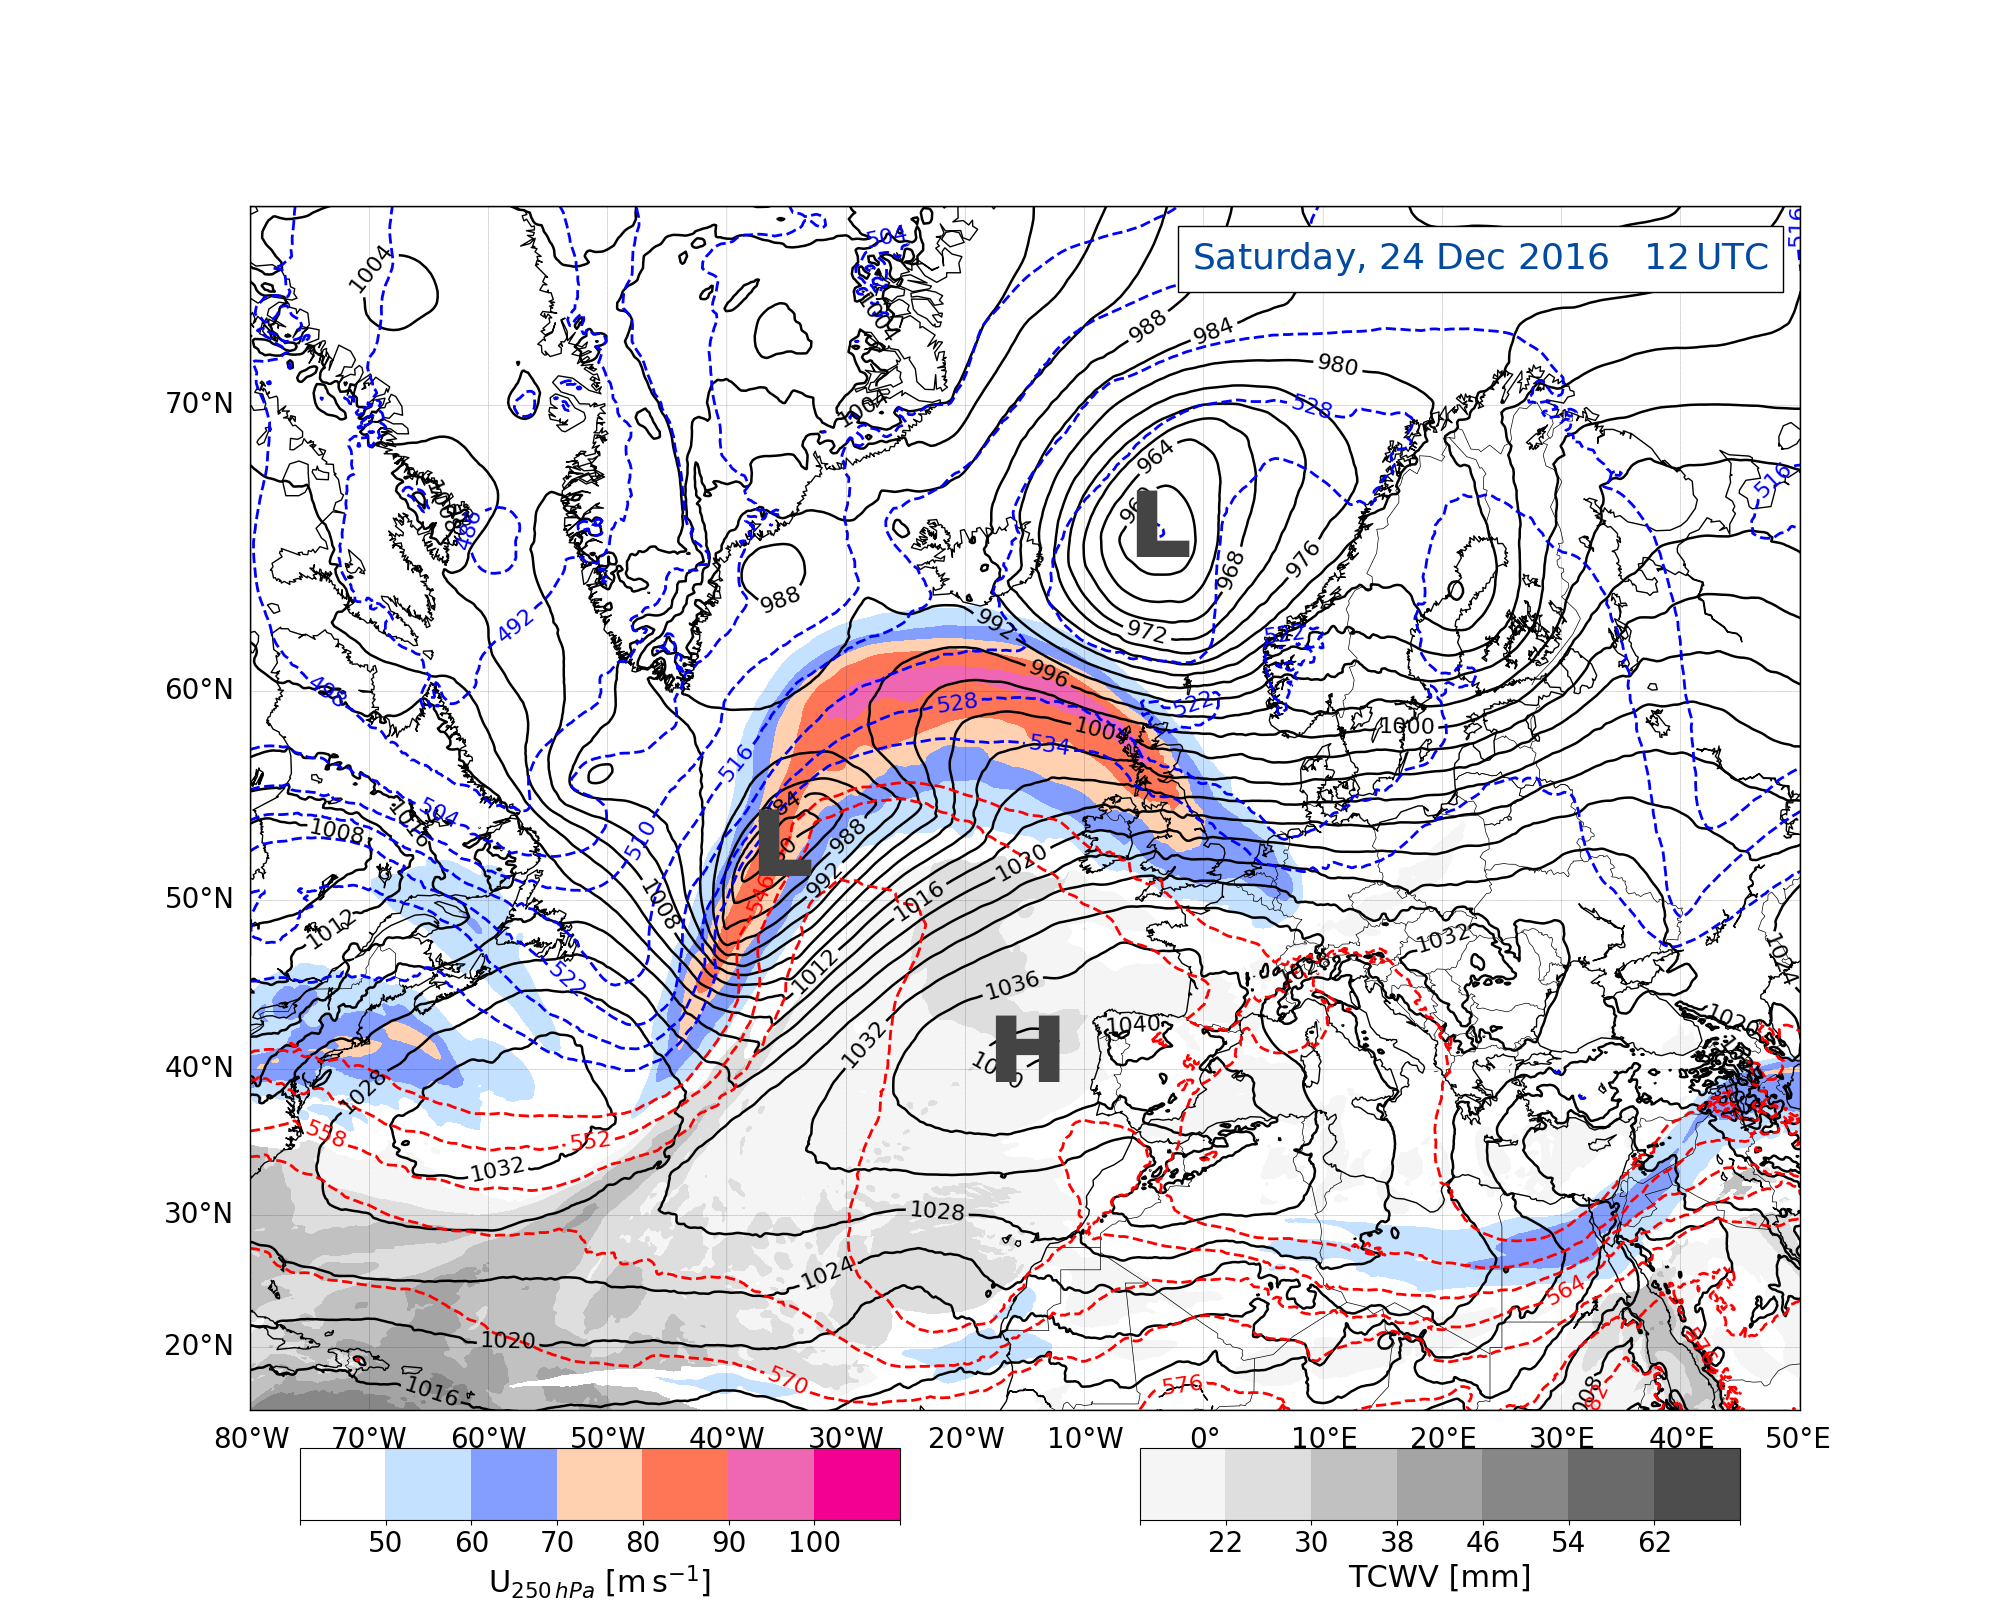
\includegraphics[trim={4.2cm 0cm 4.3cm 5.1cm},clip,
         width=\textwidth]{./fig_Geopot_Jet/20161224_12_pres}
\end{minipage}\hfill
\begin{minipage}[b]{.4\textwidth}
	\captionof{subfigure}{Jet, thickness, mean sea level pressure, and total precipitable water synoptic analysis. \SI{250}{\hPa} wind speed, shaded according to the colour bar, [\SI{}{\mPs}]. \SI{1000}-\SI{500}{\hPa} thickness, dashed contours every \SI{6}{\deca\meter}, MSLP, black contours every \SI{4}{\hPa}, total column water vapour [\SI{}{\mm}], shaded according the grey scale.} \label{fig:GP24_pres}
\end{minipage}
%%%%%% 20/12 IVT
\noindent\begin{minipage}%[t][0.55\textheight]
[t]{.59\textwidth}
  	\centering
  		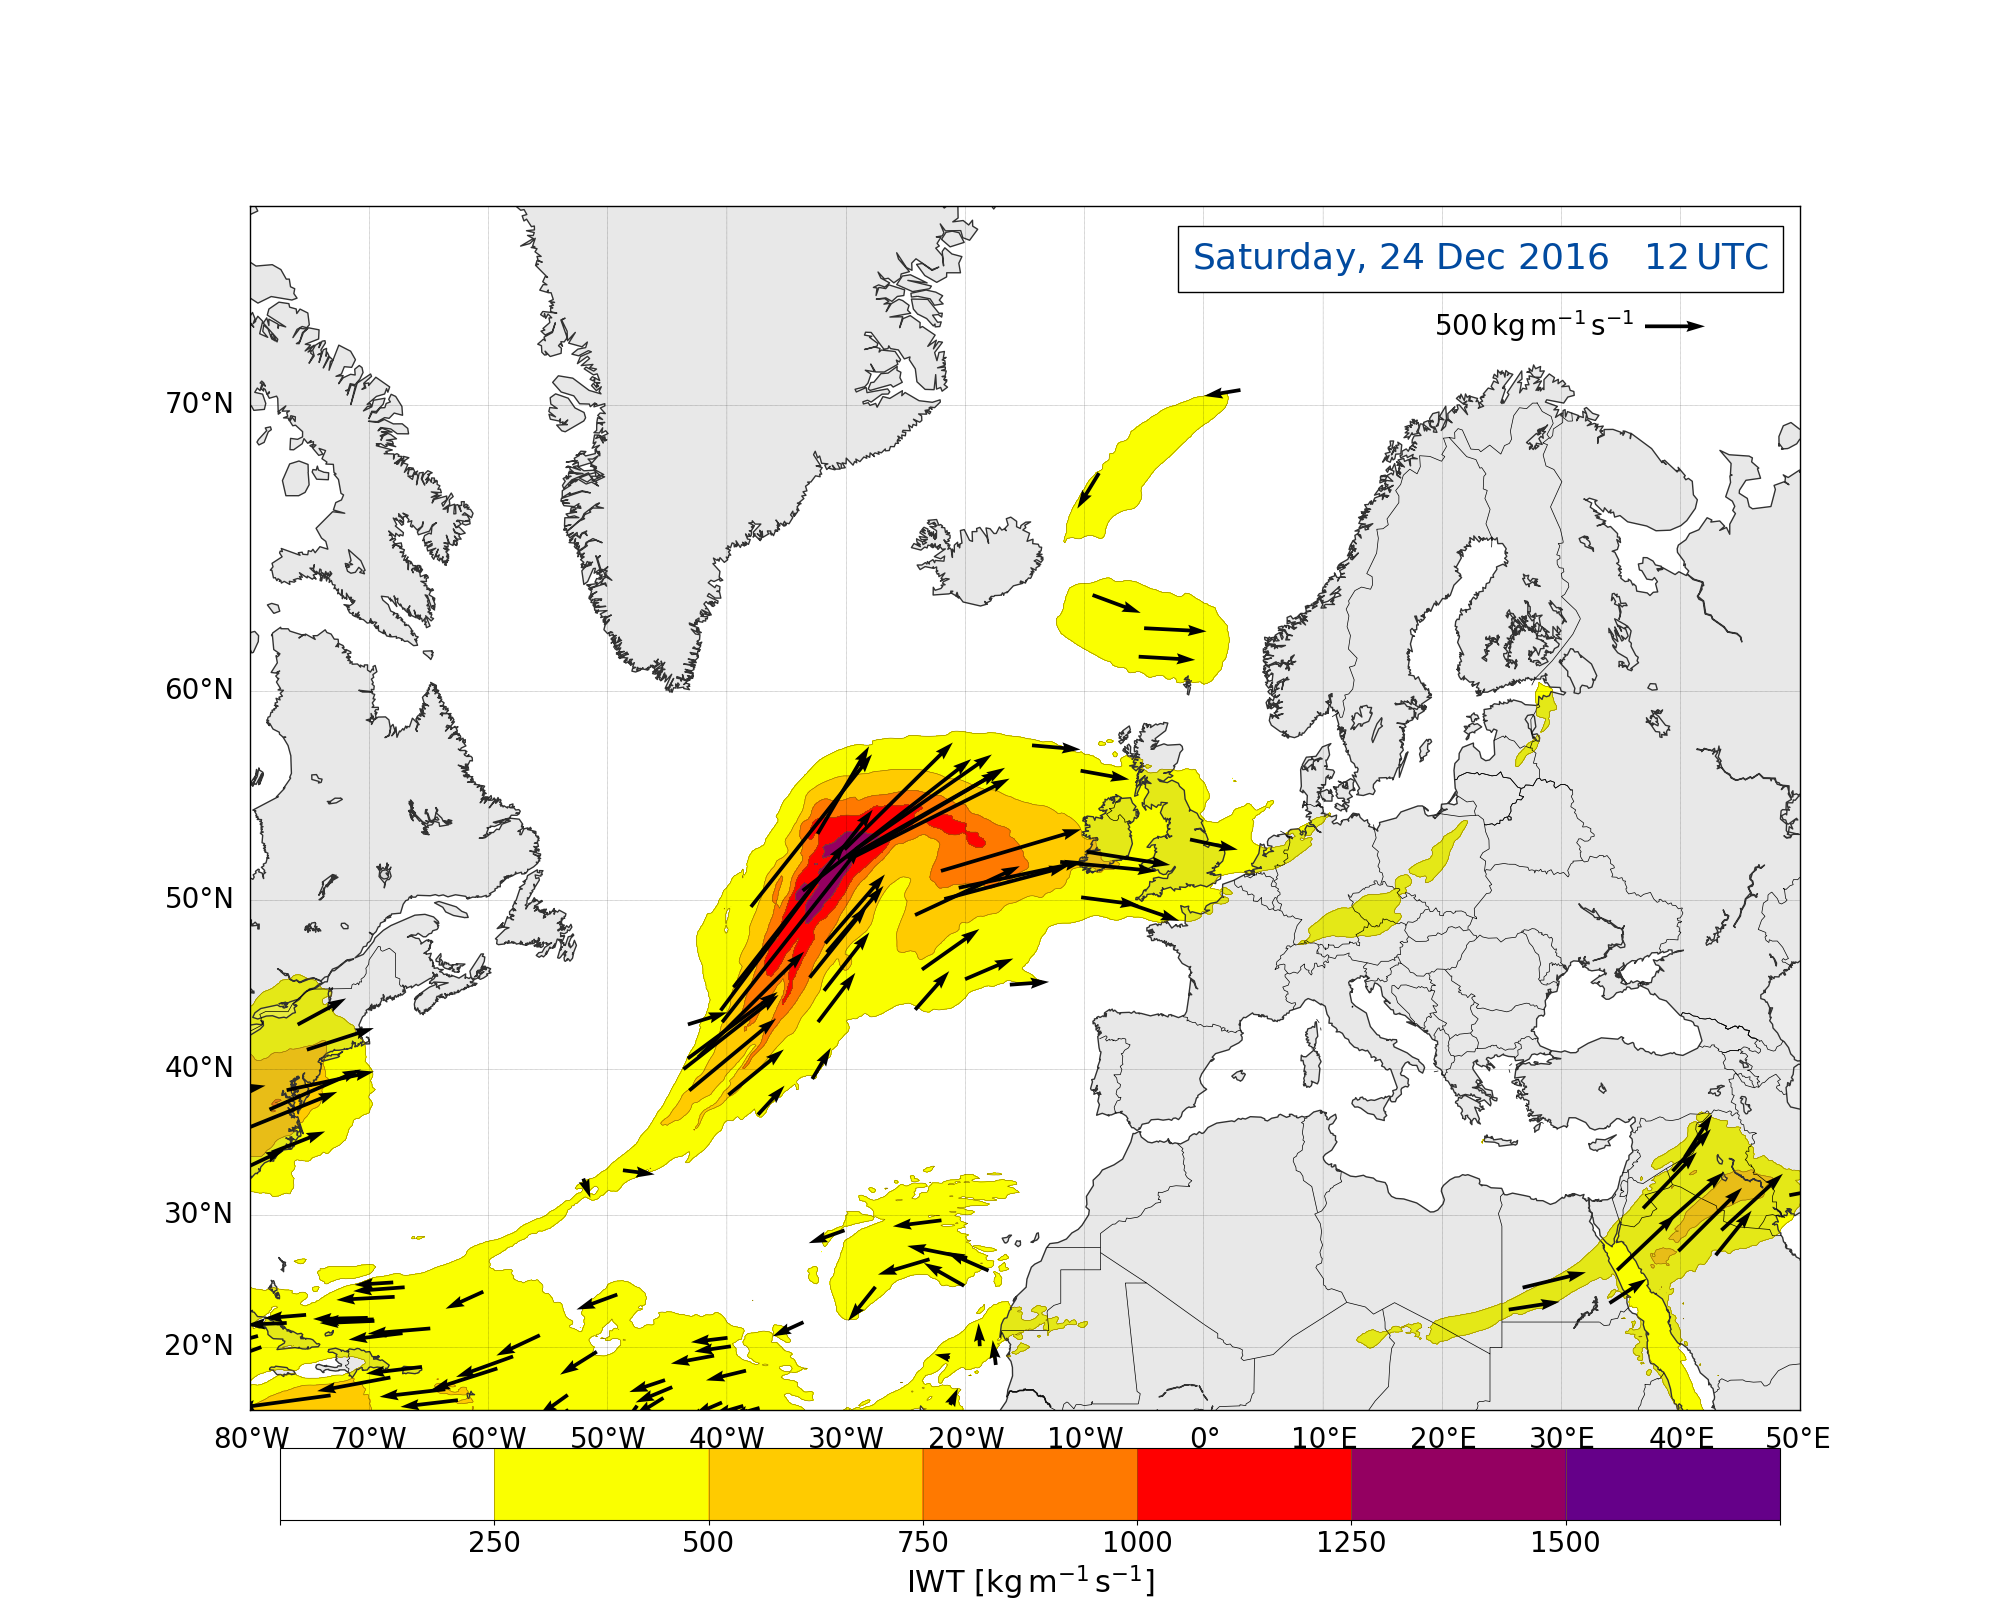
\includegraphics[trim={4.2cm 0cm 4.3cm 5.1cm},clip,
         width=\textwidth]{./fig_Atm_Riv/20161224_12}
\end{minipage}\hfill
\begin{minipage}[b]{.4\textwidth}
	\captionof{subfigure}{Integrated vapour transport analysis map. Integrated vapour transport, shaded according to the colour bar [\SI{}{\IVT}]. Vectors, indicating the direction and magnitude of the IVT. } \label{fig:AR24_pres}
\end{minipage}
\captionof{figure}{ECMWF analysis on \SI{24}{\dec} at \SI{12}{\UTC}. L and H indicating the surface low and high pressure, respectively.}\label{fig:24_12_pres}
%%%%%%%%%%%%%%%%%%%%%%%%%%%%%%%%%%%%%%%%%%%%%%%%%%%%%%%%%%%%%%%%%%%%%%%%%

%%%%%%%%% ATM_RIV %%%%%%%%%%%%%%
% !TeX spellcheck = en_GB
\section{Integrated Vapour Transport}
\label{sec:atm_riv}
% %%% Atmospheric river maps %%%%%%%%%%%%%%%%%%%%%%%%%%%%%%%%%%%%%
% % !TeX spellcheck = en_GB
\begin{figure}[h!]
	\centering
	%%%%%% 20/12
	\begin{subfigure}[b]{0.49\textwidth}
		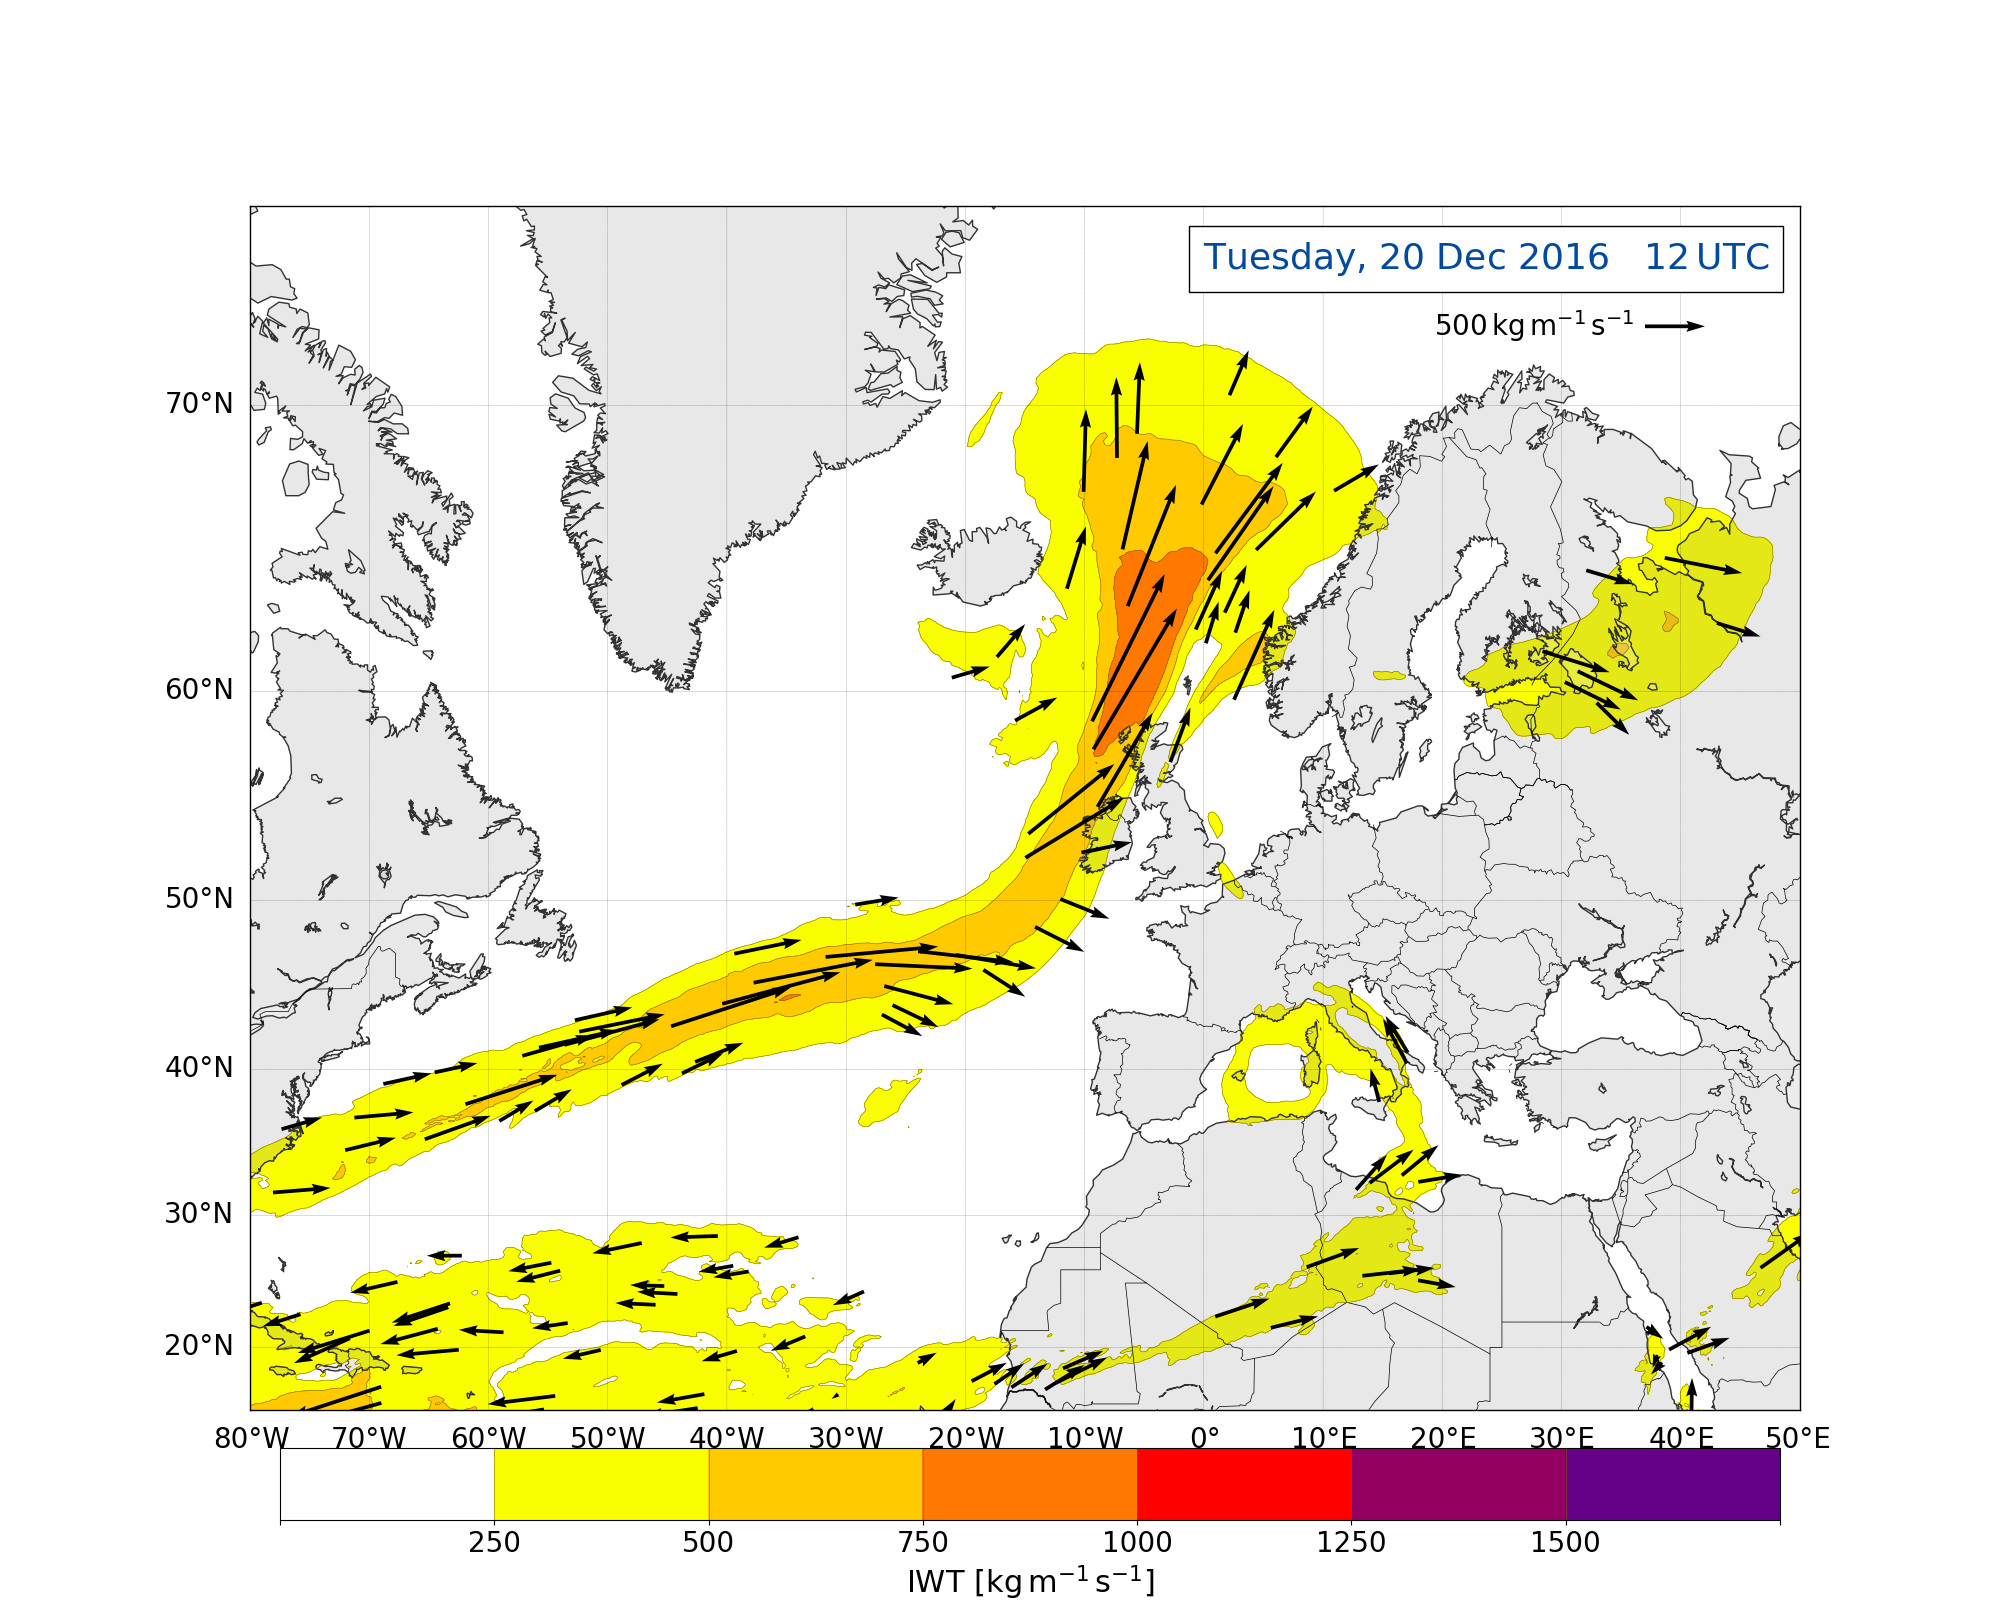
\includegraphics[trim={4.2cm 3.9cm 4.3cm 5.1cm},clip,
		width=\textwidth]{./fig_Atm_Riv/20161220_12}
		\caption{}\label{fig:AR20}
	\end{subfigure}
	%%%%%% 21/12
	\begin{subfigure}[b]{0.49\textwidth}
		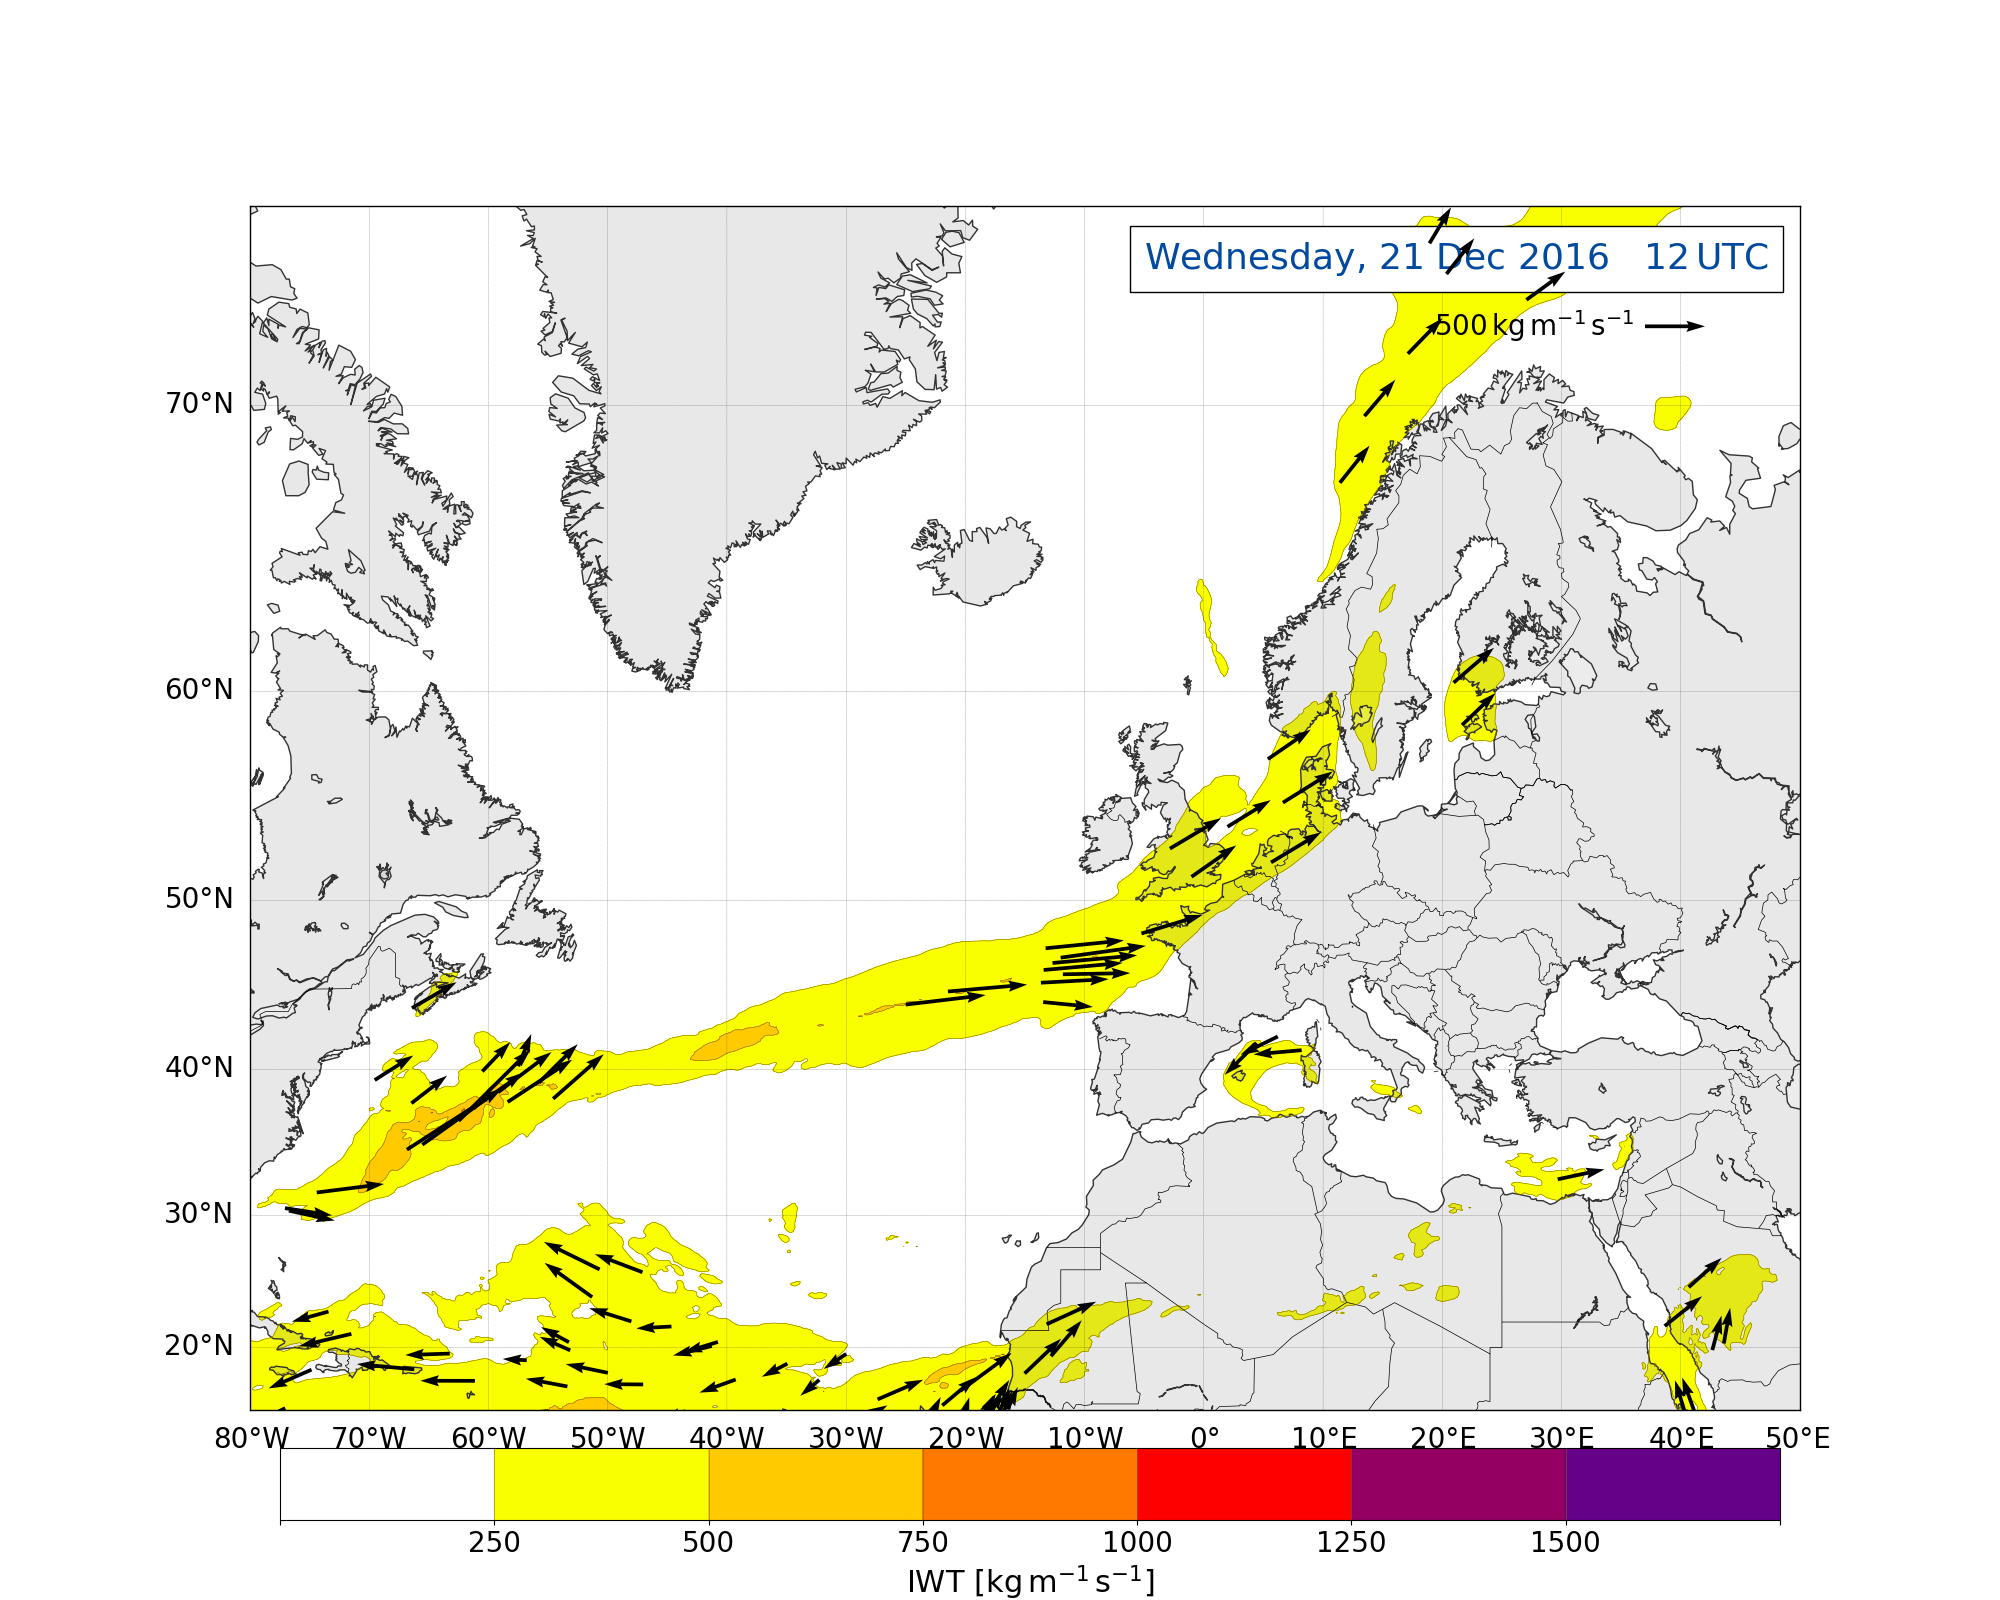
\includegraphics[trim={4.2cm 3.9cm 4.3cm 5.1cm},clip,
		width=\textwidth]{./fig_Atm_Riv/20161221_12}
		\caption{}\label{fig:AR21}
	\end{subfigure}
	%%%%%% label
	\begin{subfigure}[b]{\textwidth}
		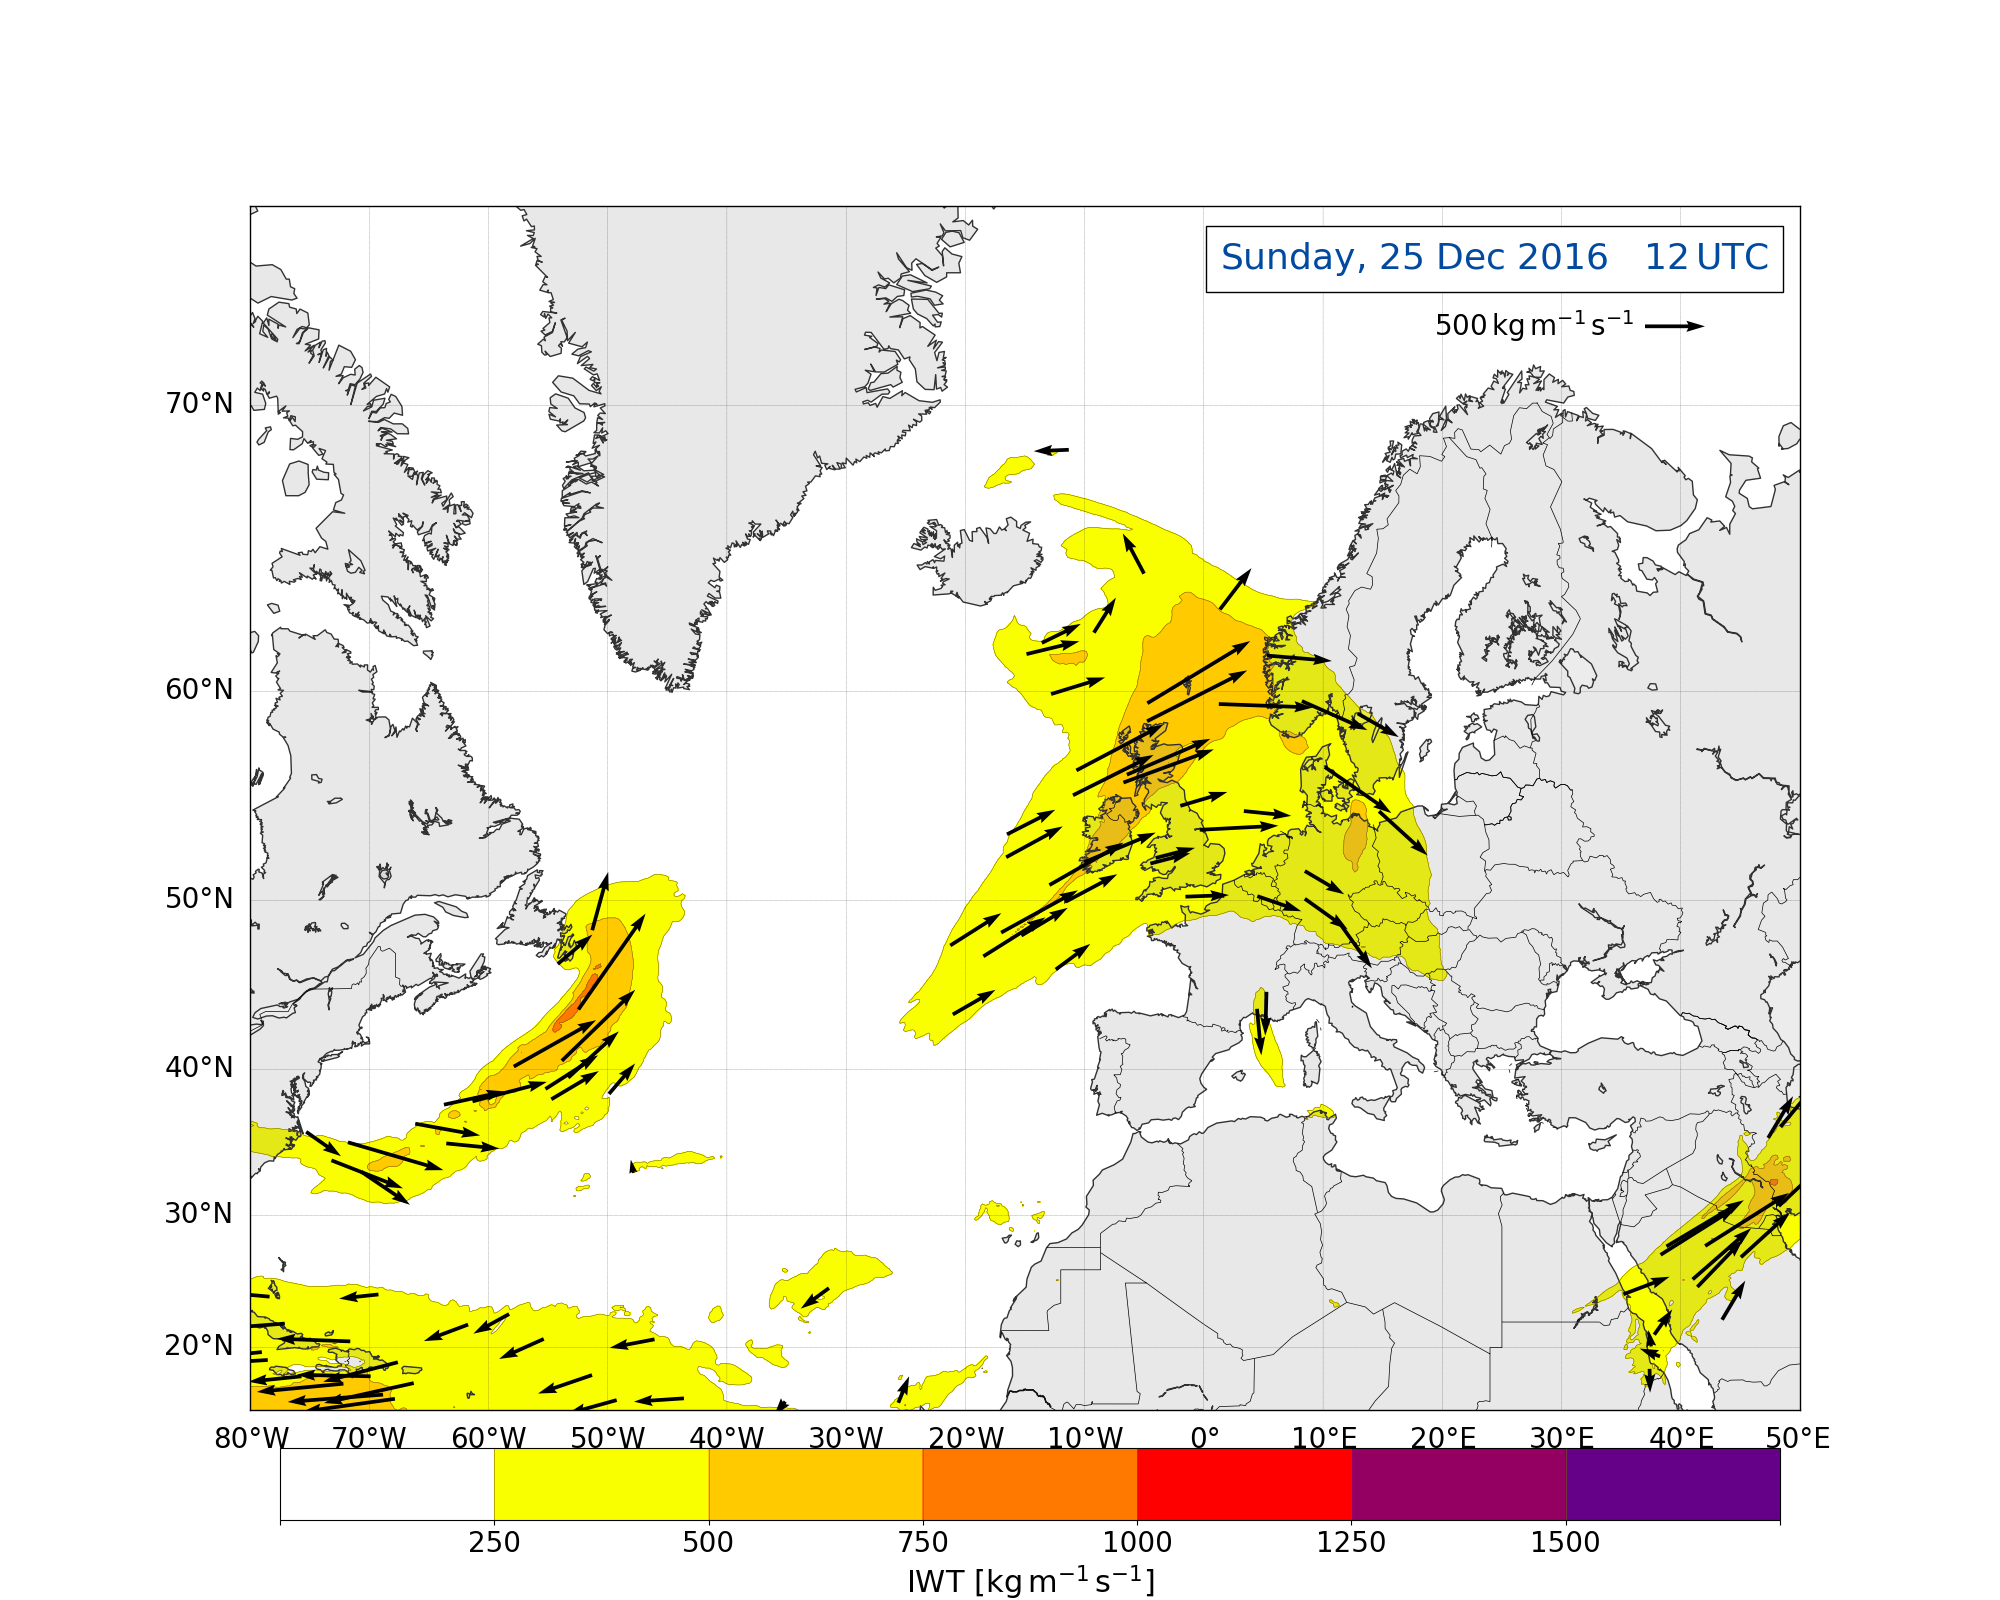
\includegraphics[trim={4.2cm 0cm 4.3cm 36.8cm},clip,
		width=\textwidth]{./fig_Atm_Riv/20161225_12}
	\end{subfigure}
\end{figure}
%
\begin{figure}\ContinuedFloat
	\centering
	%%%%%% 22/12
	\begin{subfigure}[b]{0.49\textwidth}
		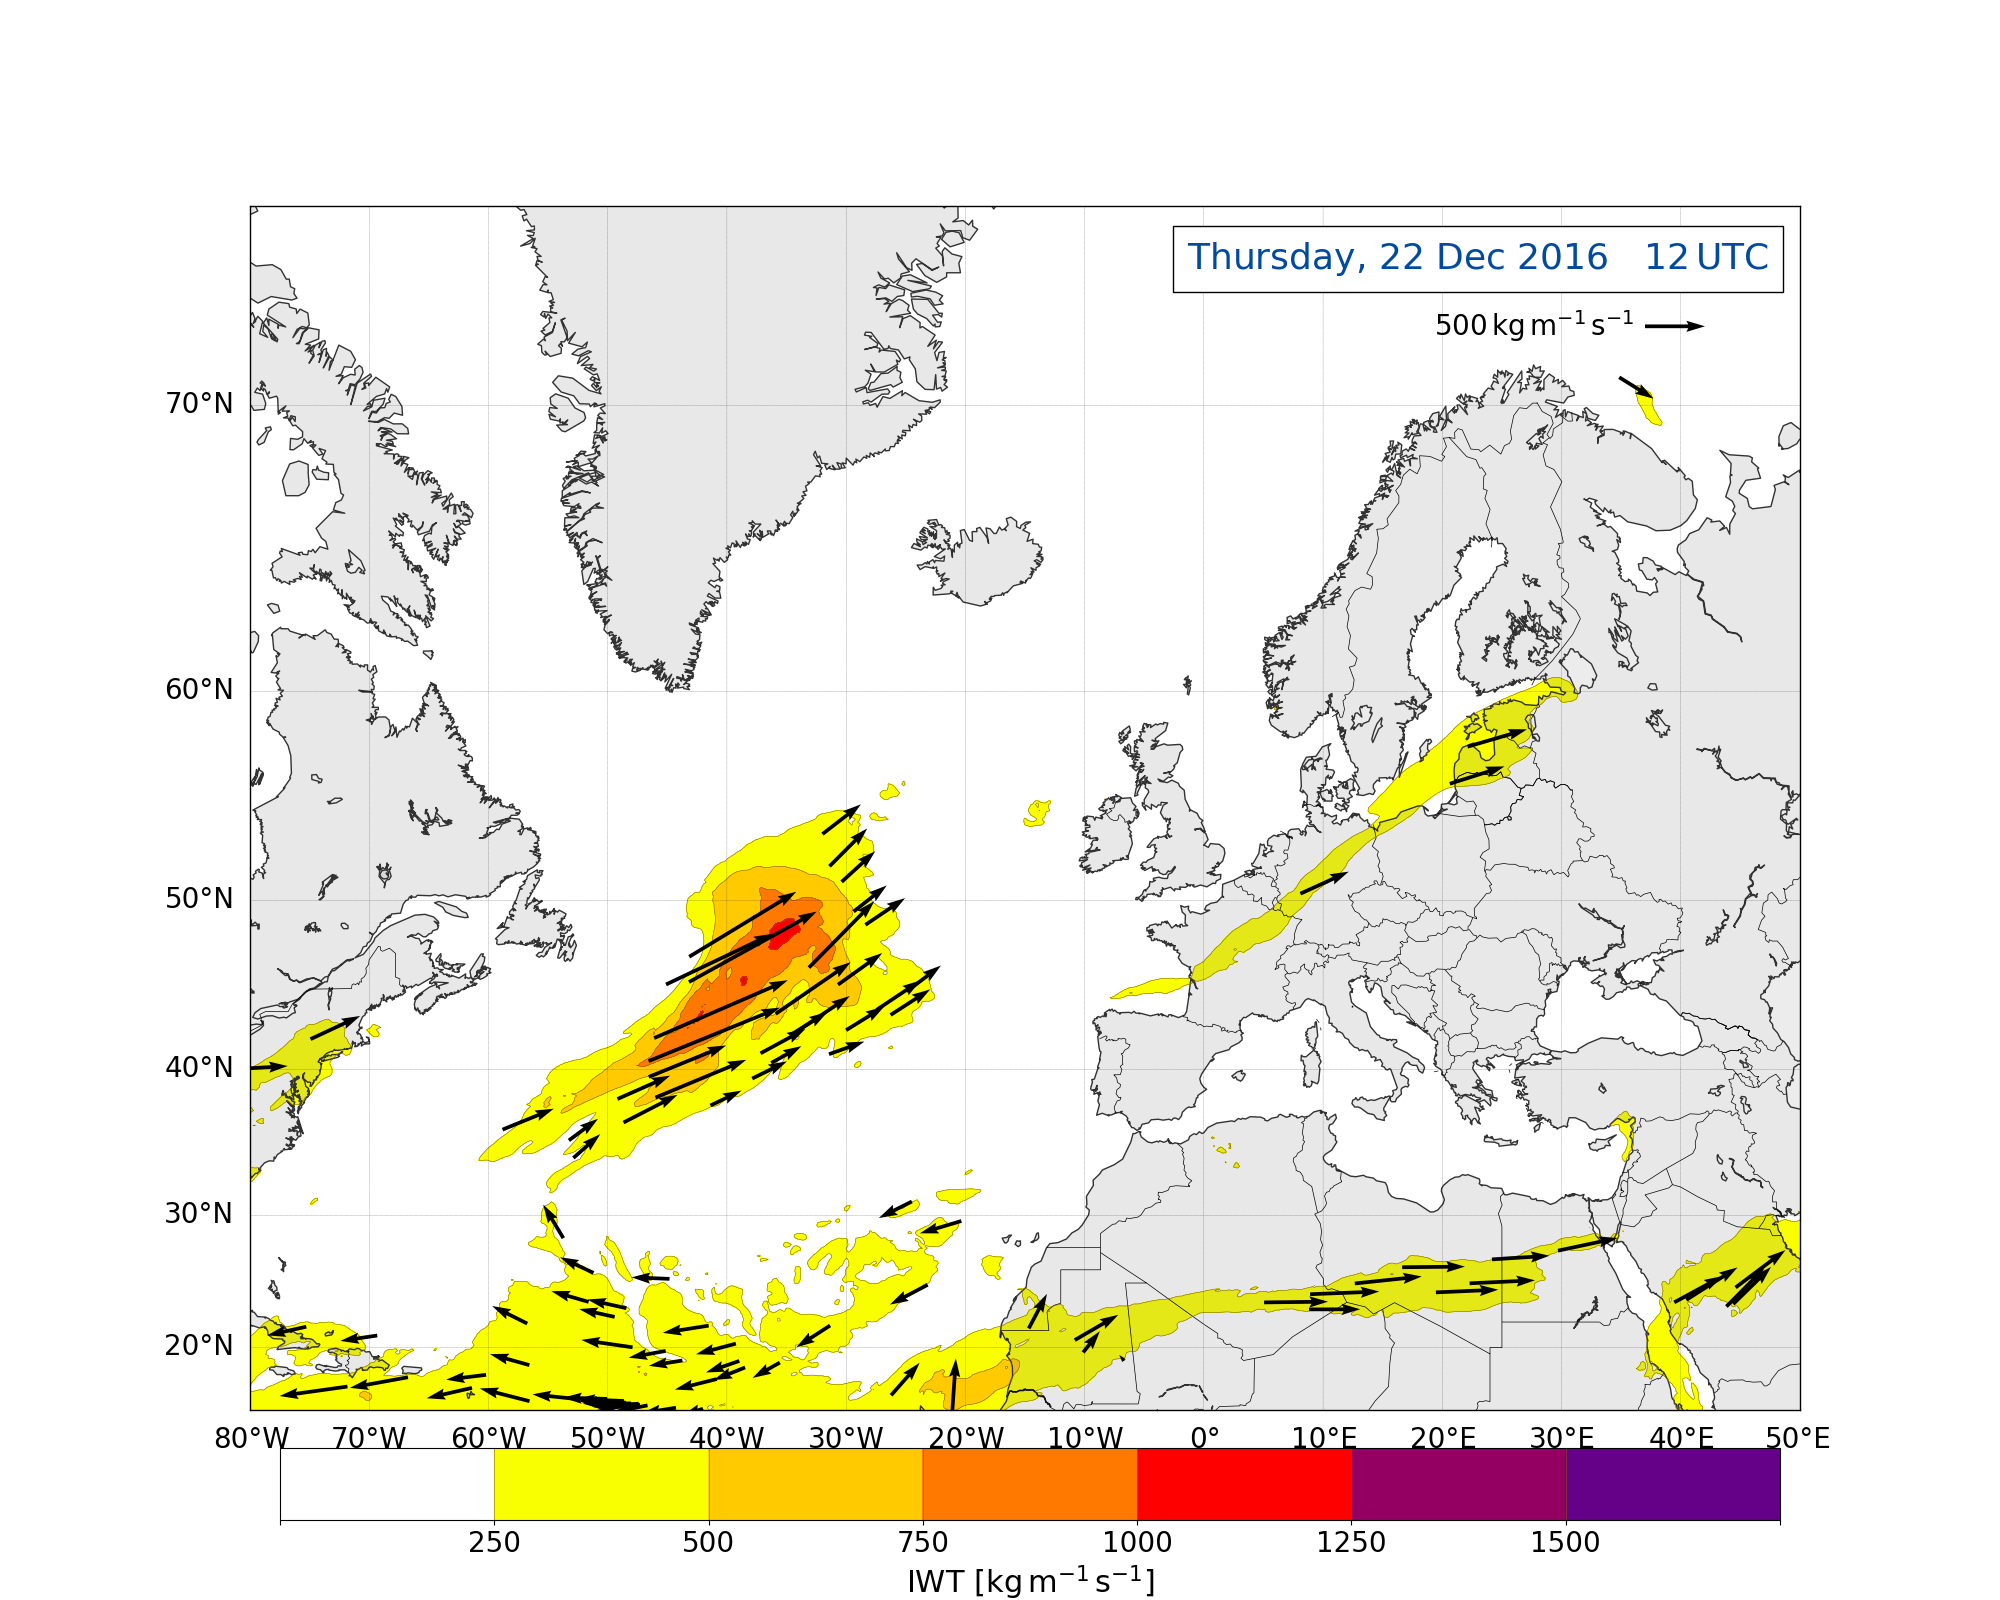
\includegraphics[trim={4.2cm 3.9cm 4.3cm 5.1cm},clip,
		width=\textwidth]{./fig_Atm_Riv/20161222_12}
		\caption{}\label{fig:AR22}
		%\label{fig:sfc2100}
	\end{subfigure}
	%%%%%% 23/12
	\begin{subfigure}[b]{0.49\textwidth}
		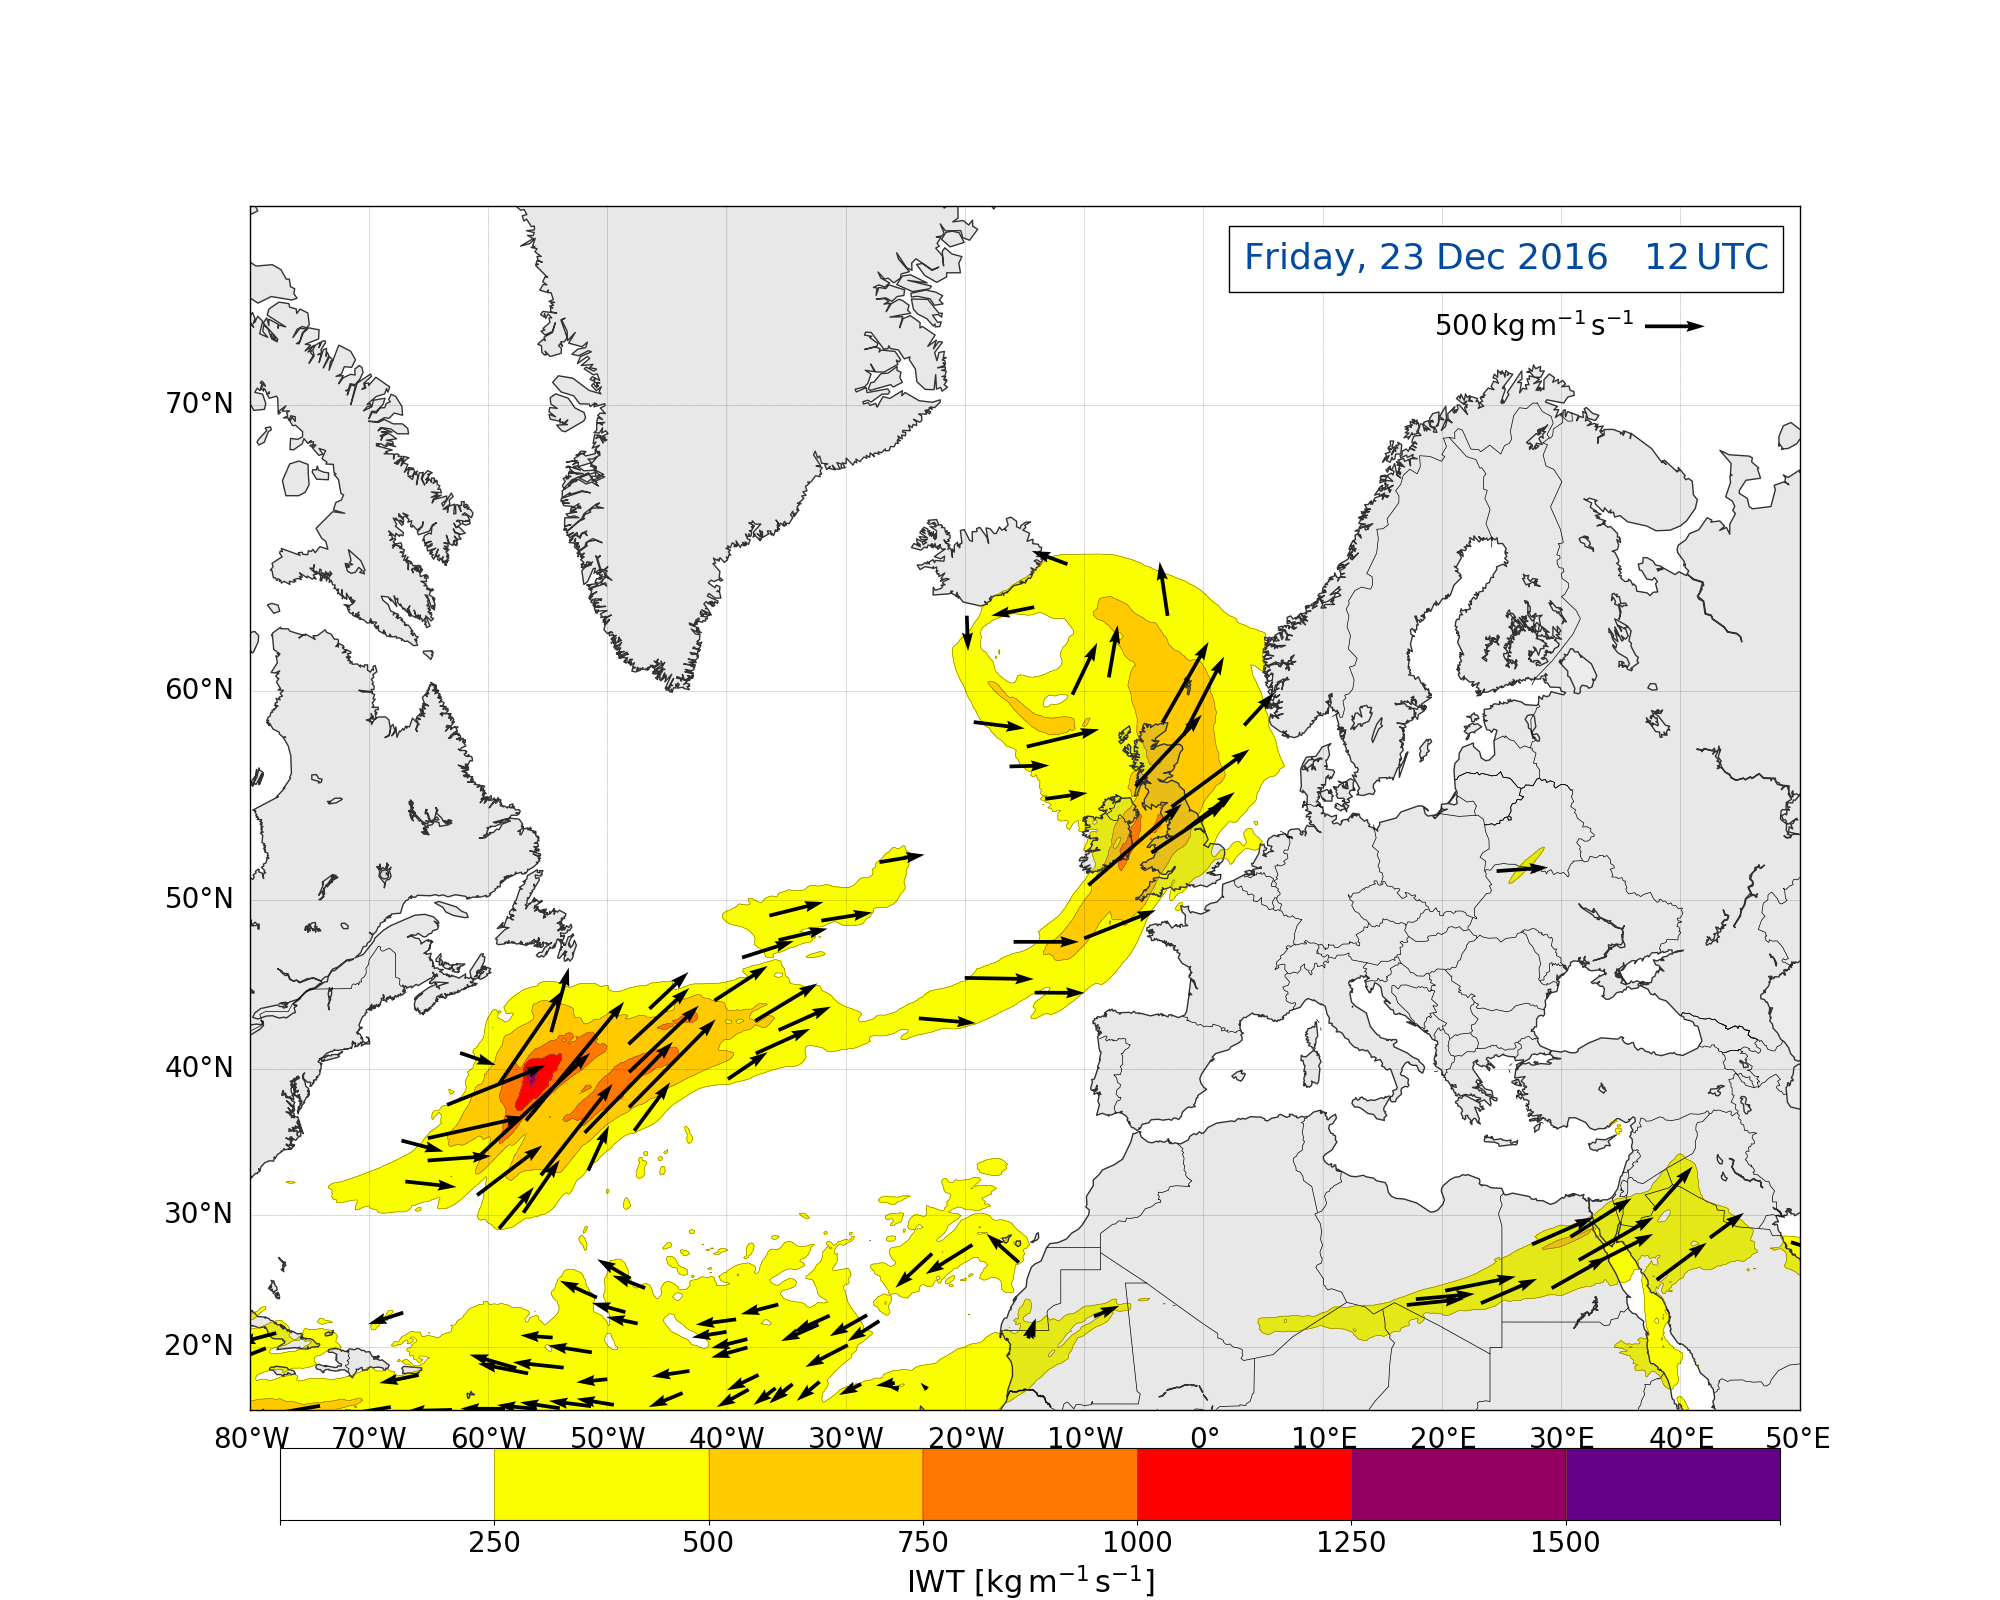
\includegraphics[trim={4.2cm 3.9cm 4.3cm 5.1cm},clip,
		width=\textwidth]{./fig_Atm_Riv/20161223_12}
		\caption{}\label{fig:AR23}
	\end{subfigure}
	%%%%%% 24/12
	\begin{subfigure}[b]{0.49\textwidth}
		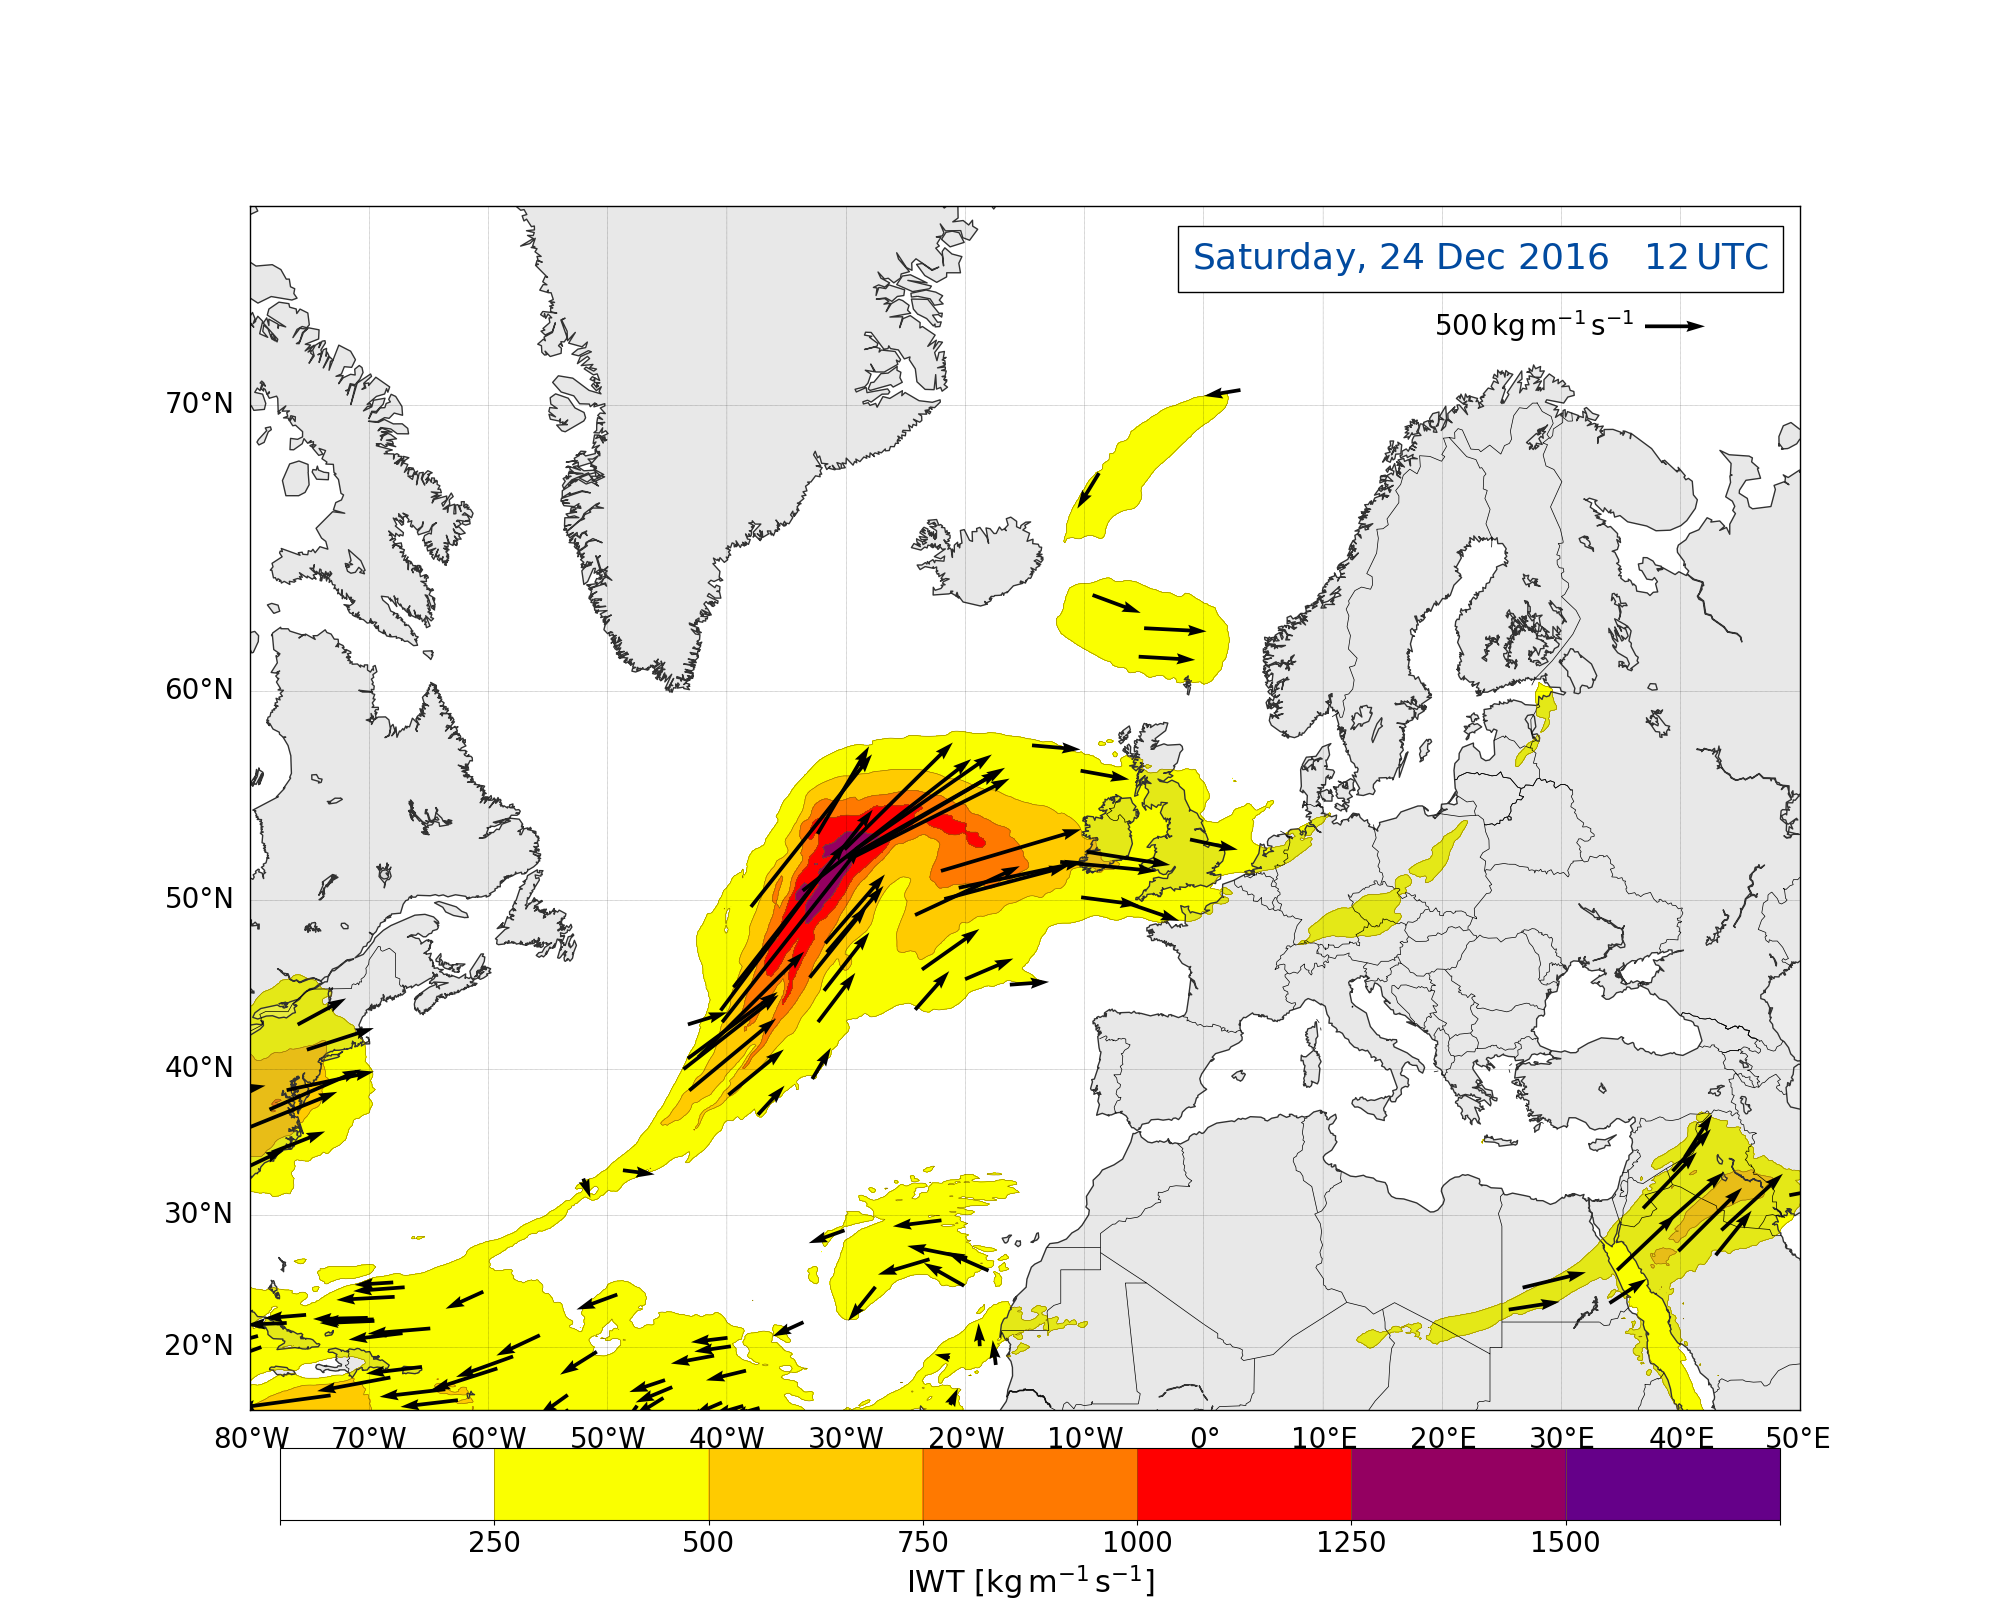
\includegraphics[trim={4.2cm 3.9cm 4.3cm 5.1cm},clip,
		width=\textwidth]{./fig_Atm_Riv/20161224_12}
		\caption{}\label{fig:AR24}
	\end{subfigure}
	%%%%%% 25/12
	\begin{subfigure}[b]{0.49\textwidth}
		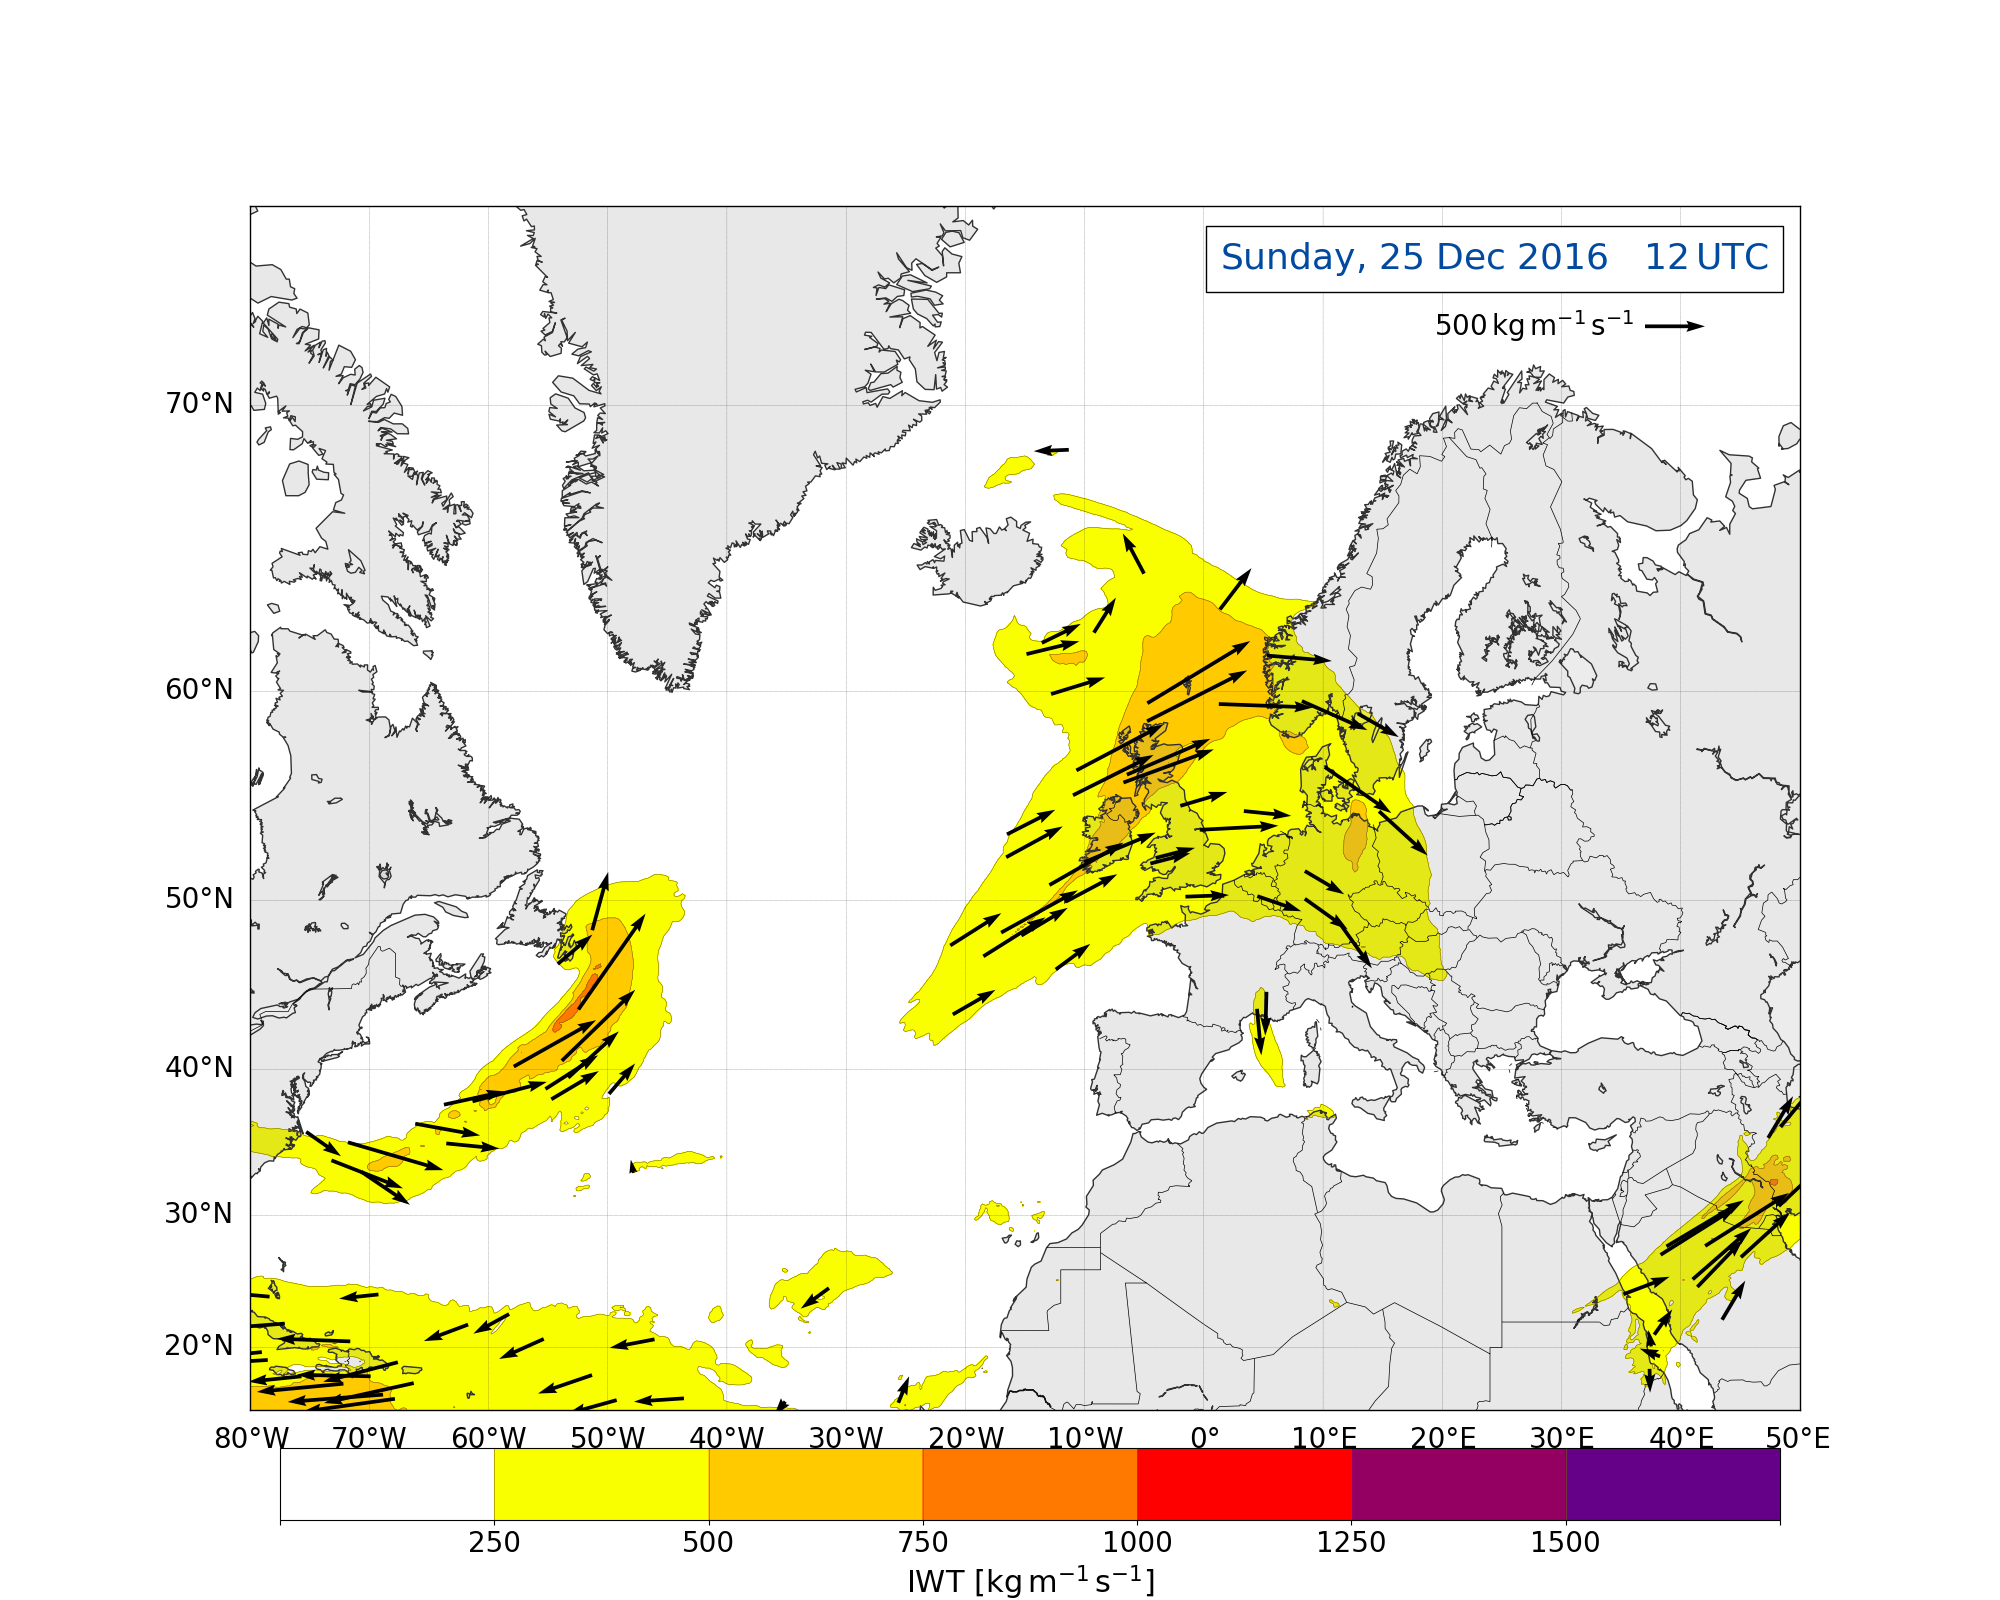
\includegraphics[trim={4.2cm 3.9cm 4.3cm 5.1cm},clip,
		width=\textwidth]{./fig_Atm_Riv/20161225_12}
		\caption{}\label{fig:AR25}
	\end{subfigure}
	%	\centering
	%%%%%% 26/12
	\begin{subfigure}[b]{0.49\textwidth}
		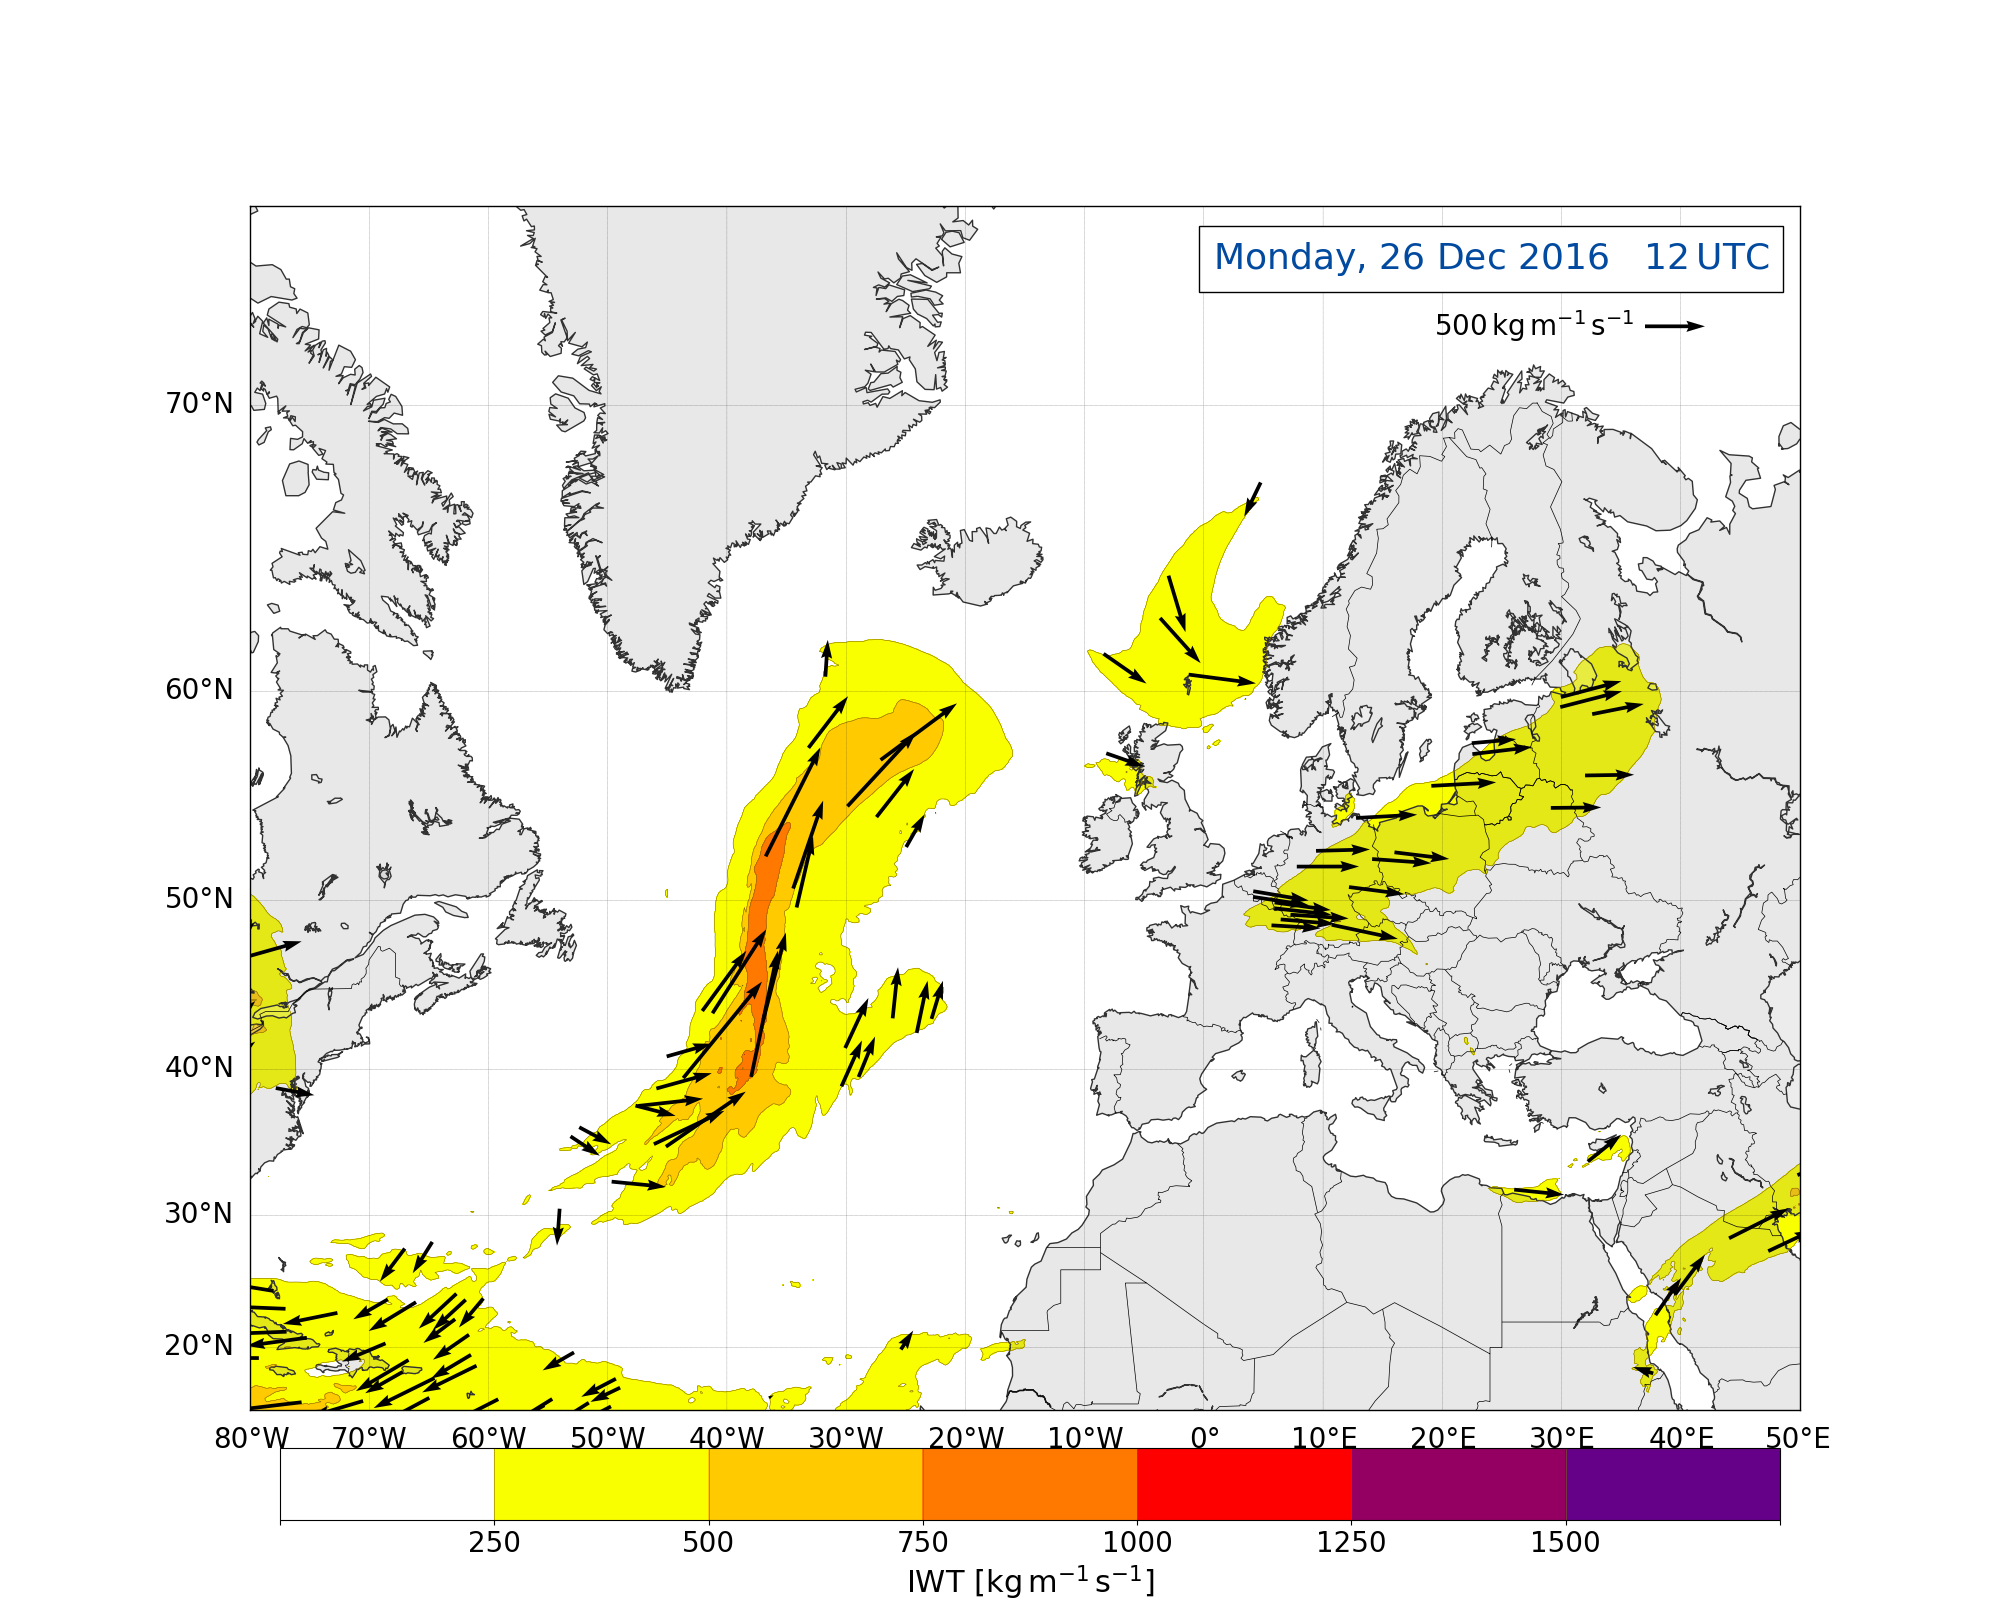
\includegraphics[trim={4.2cm 3.9cm 4.3cm 5.1cm},clip,
		width=\textwidth]{./fig_Atm_Riv/20161226_12}
		\caption{}\label{fig:AR26}
	\end{subfigure}
	%%%%%% 27/12
	\begin{subfigure}[b]{0.49\textwidth}
		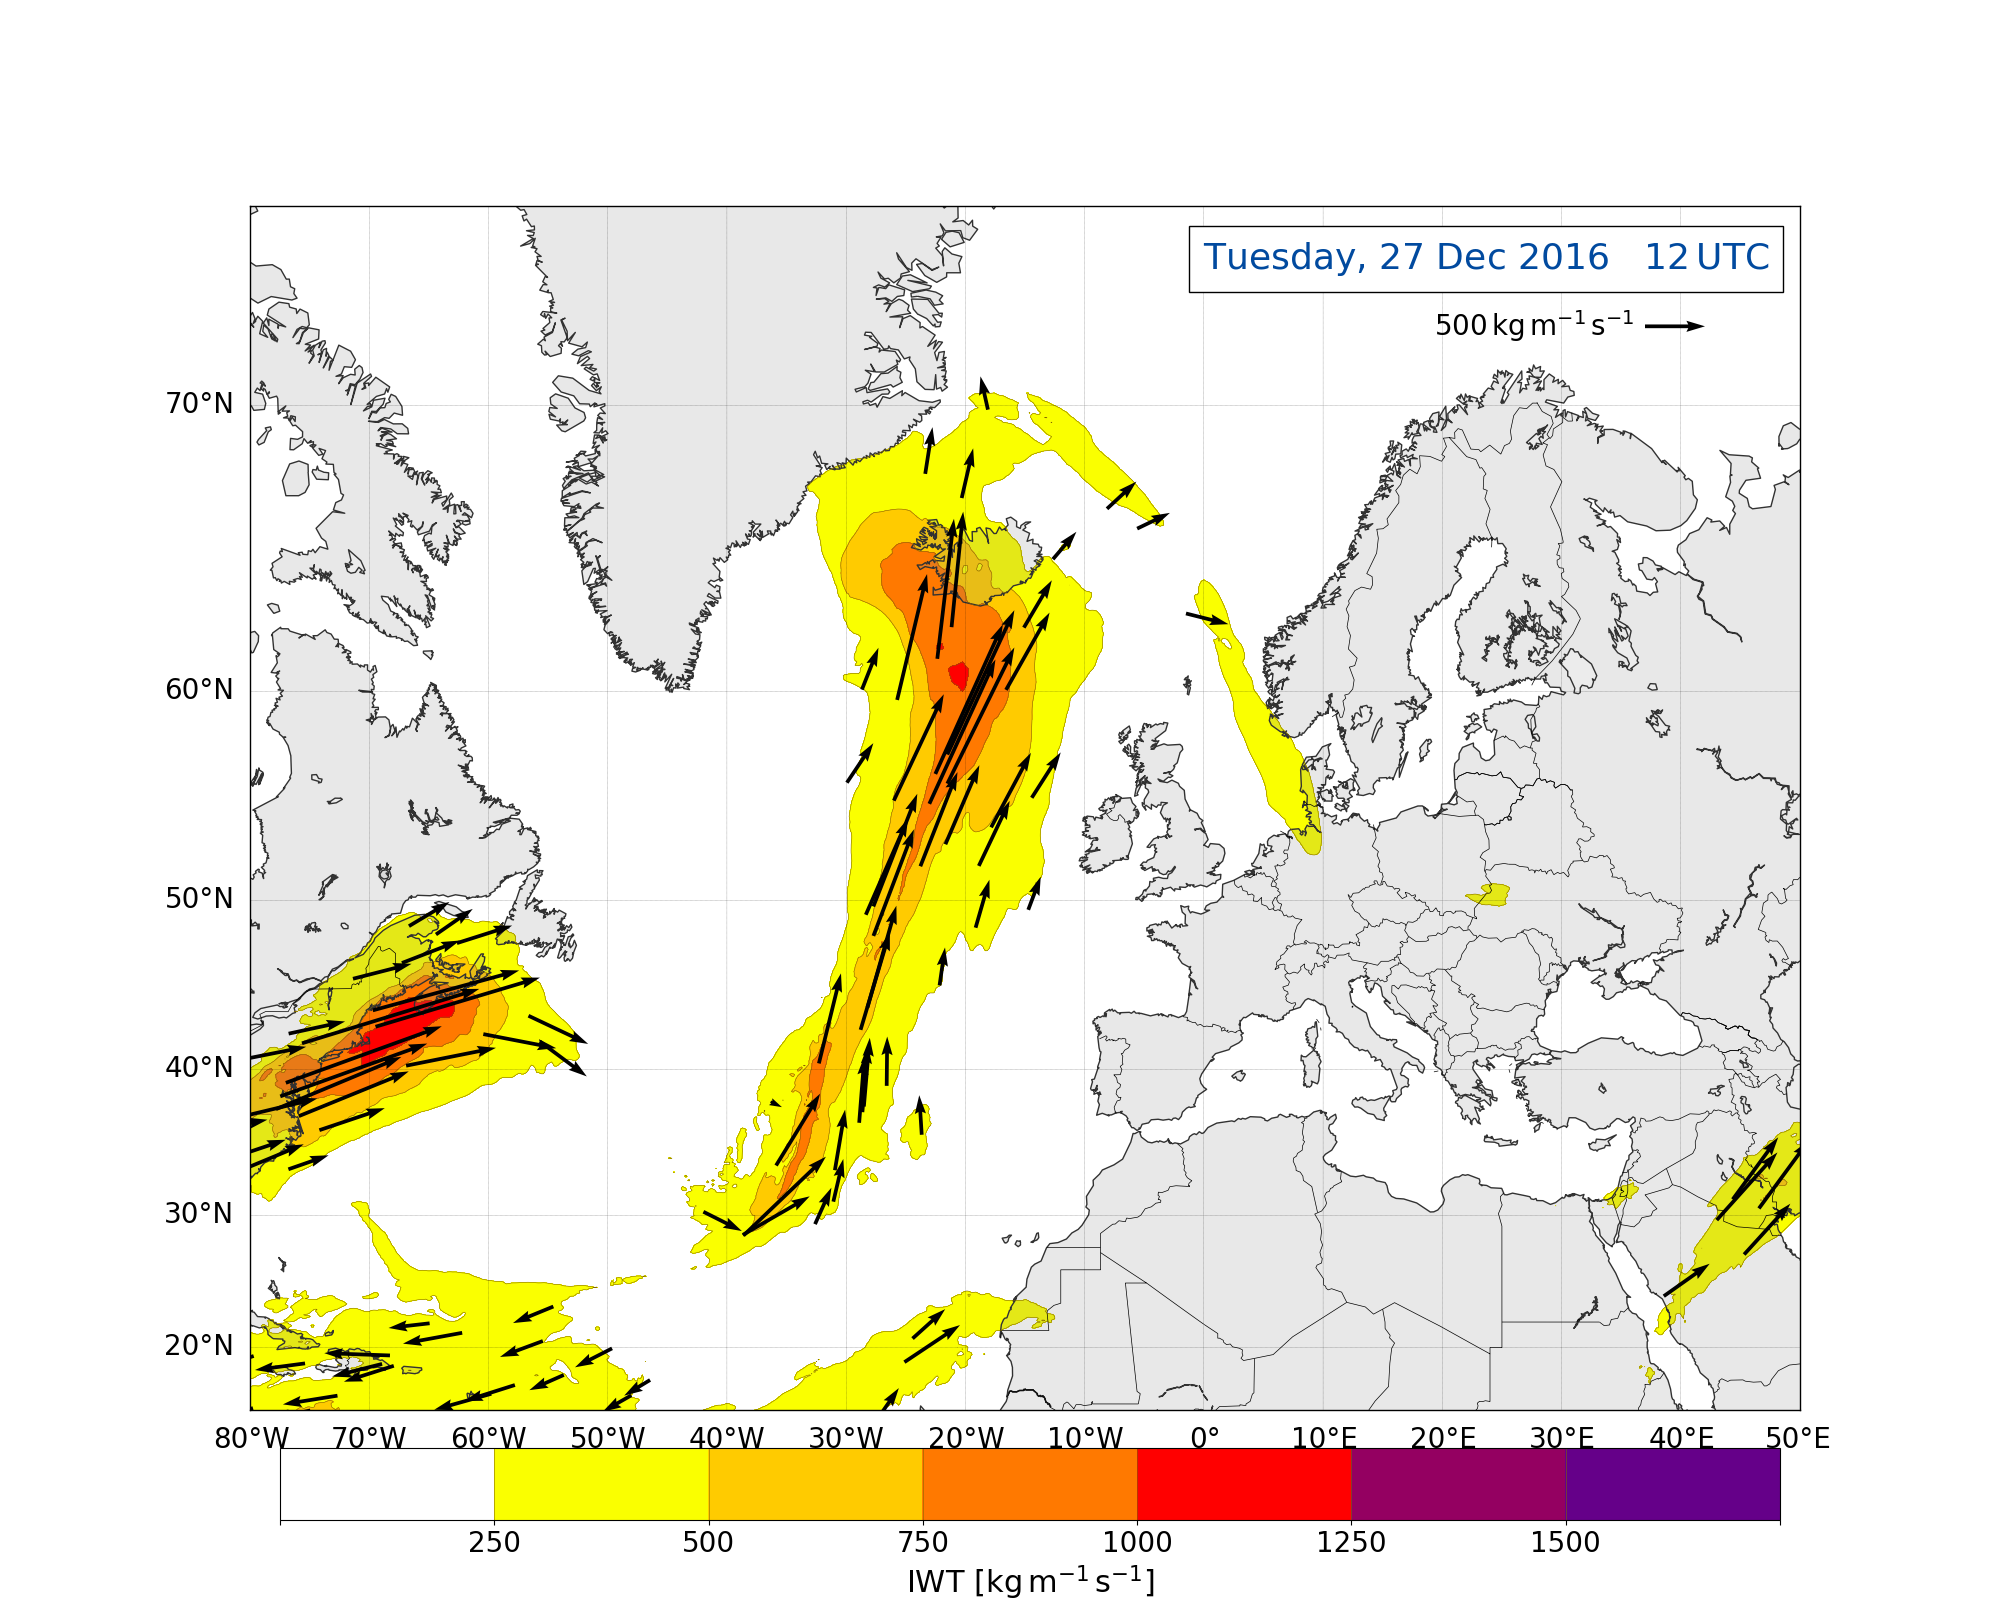
\includegraphics[trim={4.2cm 3.9cm 4.3cm 5.1cm},clip,
		width=\textwidth]{./fig_Atm_Riv/20161227_12}
		\caption{}\label{fig:AR27}
	\end{subfigure}
	%%%%%% label
	\begin{subfigure}[b]{\textwidth}
		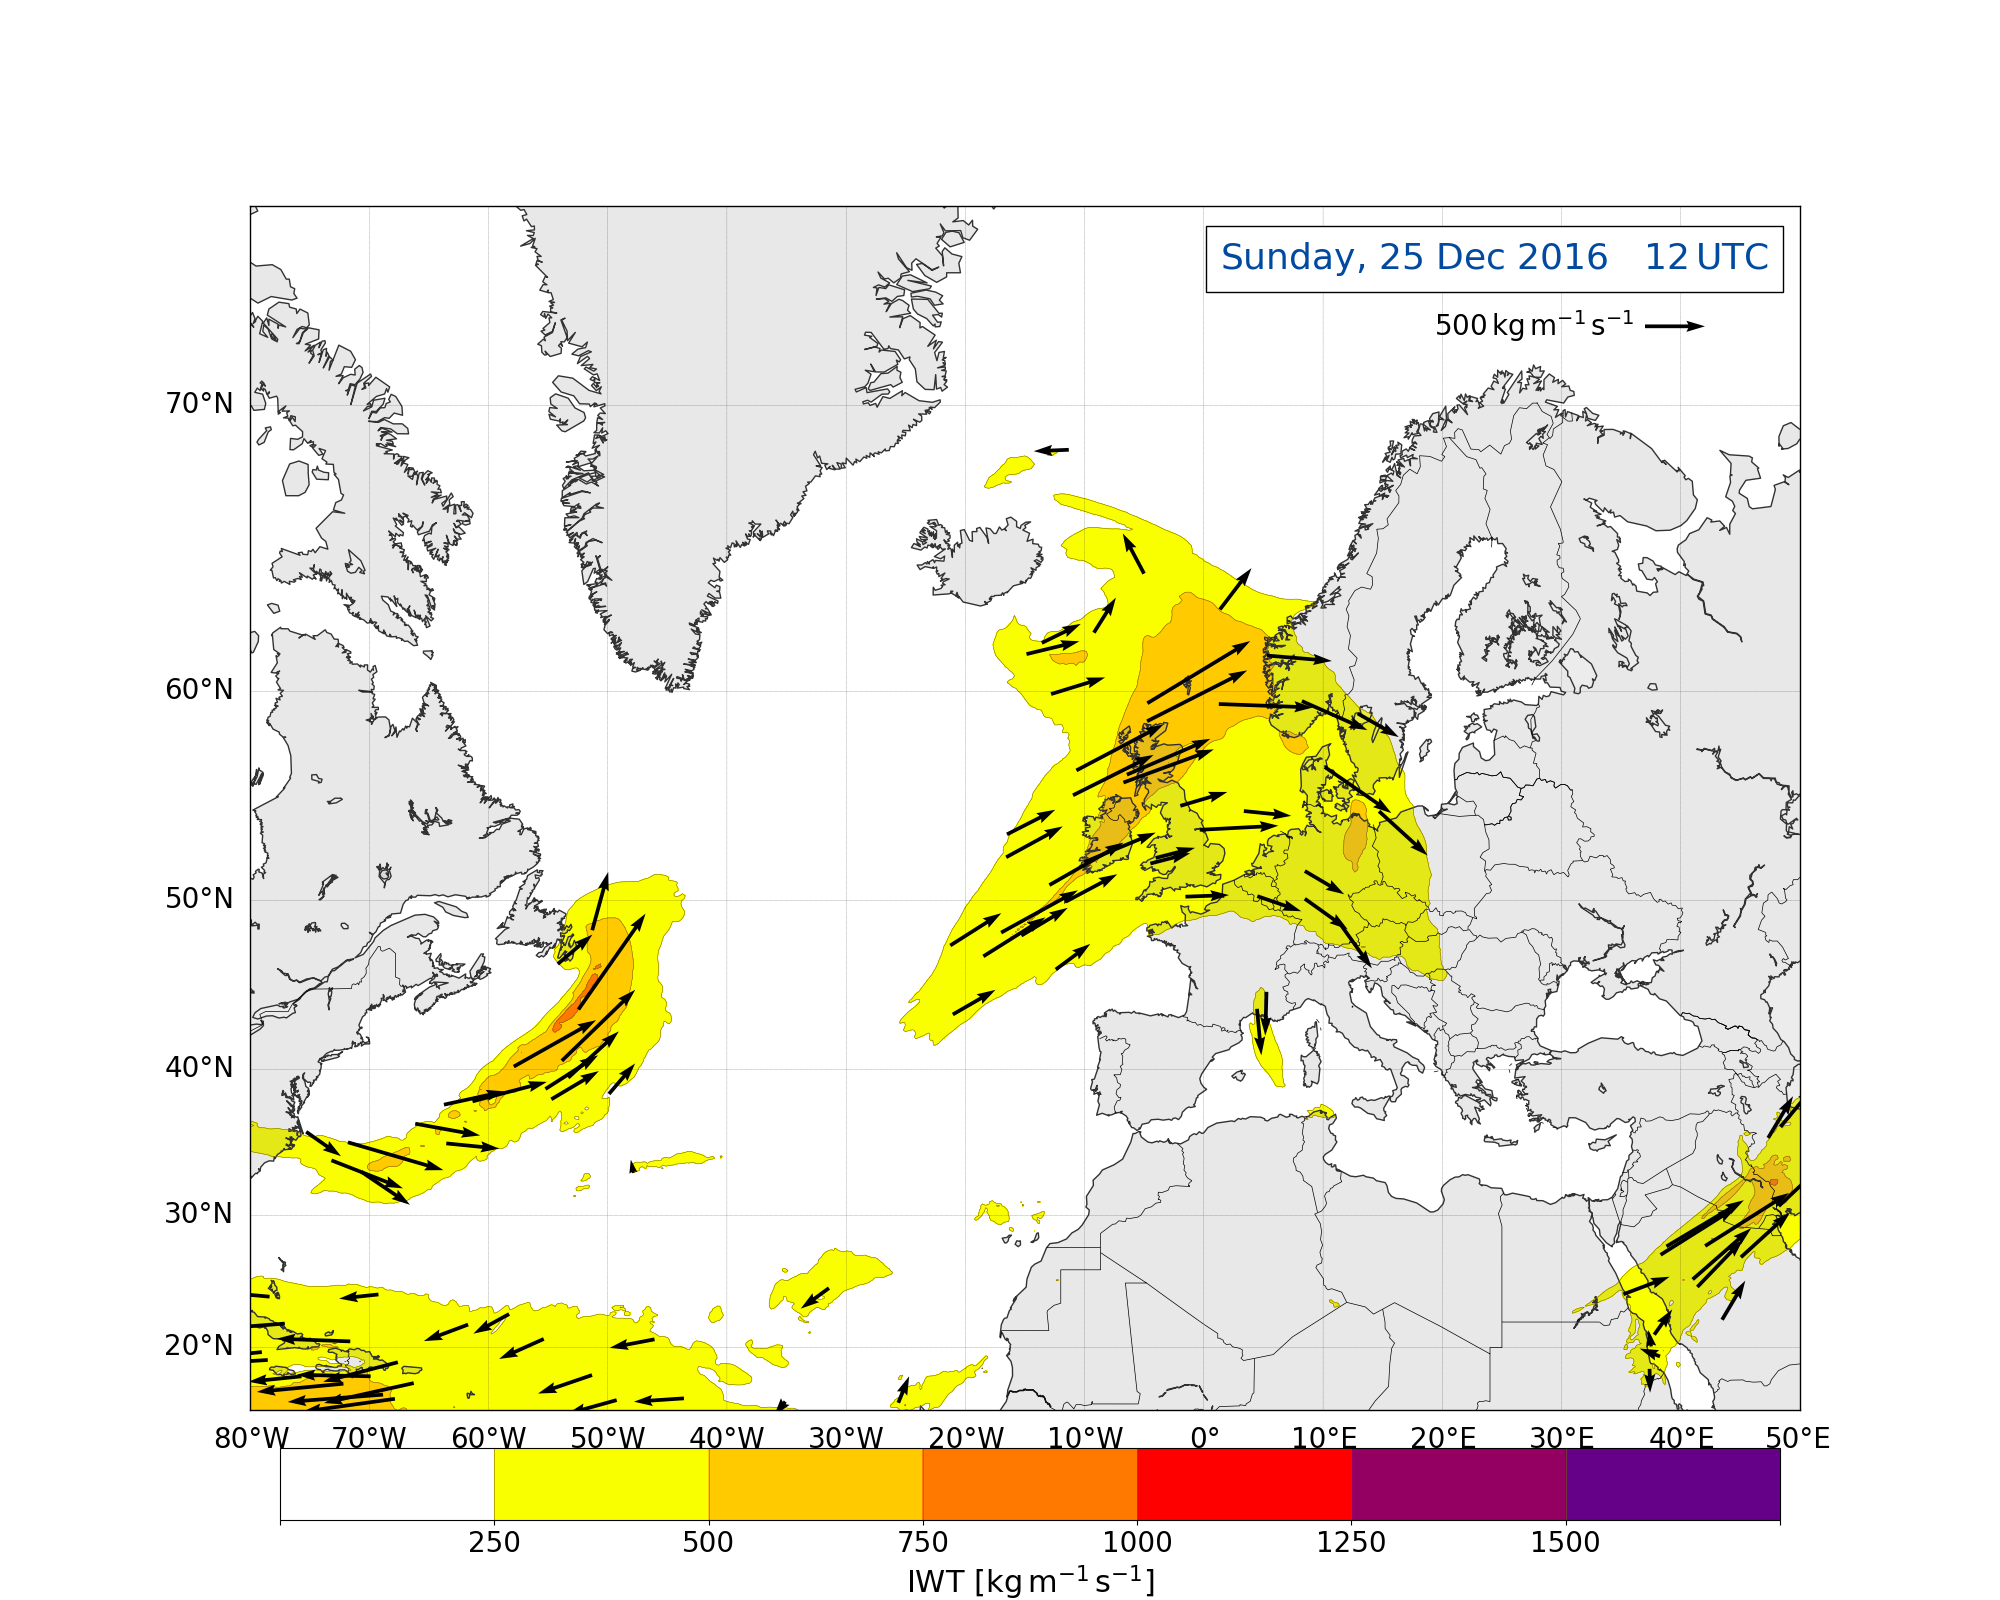
\includegraphics[trim={4.2cm 0cm 4.3cm 36.8cm},clip,
		width=\textwidth]{./fig_Atm_Riv/20161225_12}
	\end{subfigure}
	\caption{Atmospheric river analysis map, data from ECMWF. During \SIrange{20}{27}{\dec}. IVT, shaded according to the colour bar [\SI{}{\IVT}]. Vectors, indicating the direction and magnitude of the IVT. }\label{fig:AtmRiv}
\end{figure}
% %%%%%%%%%%%%%%%%%%%%%%%%%%%%%%%%%%%%%%%%%%%%%%%%%%%%%%%%%%%%%%%%%%%%%%%%%%
\Cref{fig:AR24_pres} shows coloured contours of the integrated vapour transport (IVT) in \SI{}{\IVT}, where warmer colours indicate higher IVT. Stream vectors indicate the direction and intensity of the IVT flow. An atmospheric river is characterised if the integrated vapour transport shows values higher than \SI{250}{\IVT} and a continuous region larger than \SI{2000}{\km} \citep{rutz_climatological_2014}.
\\
An atmospheric river (AR) is a filament structure of intense moisture transport from the tropics to higher latitudes. 
Heavy precipitation can be associated with it, because the air is warm and moist. This can often be observed at mountain ranges at west coasts such as in Norway \textcolor{red}{include reference here}. Due to orographic lifting will the moisture be released and follow high amounts of precipitation.  
\\
The integrated vapour transport (IVT) was calculated from the ECMWF data as followed:
\begin{align}
IVT = \frac{1}{g} \int\limits_{p_{sfc}}^{\SI{100}{\hPa}} q \mathbf{V} dp \qquad [\SI{}{\IVT}]
\label{eq:IVT}
\end{align} 
where $g$ is the standard gravity, $q$ the specific humidity, and $\mathbf{V}$ the total wind vector at each pressure level $p$. The numerical, trapezoidal integration is performed by using data from the surface pressure $p_{sfc}$ to \SI{850}{\hPa} in \SI{50}{\hPa} intervals and from \SIrange{700}{100}{\hPa} in \SI{100}{\hPa} intervals.
\\
\textcolor{red}{Add here something like this:
The Christmas storm was an atmospheric event, but not in the classical way, hence the atmospheric river case is not discussed in depth.}
%% Atmospheric river maps %%%%%%%%%%%%%%%%%%%%%%%%%%%%%%%%%%%%%
% !TeX spellcheck = en_GB
\begin{figure}[h!]
	\centering
	%%%%%% 20/12
	\begin{subfigure}[b]{0.49\textwidth}
		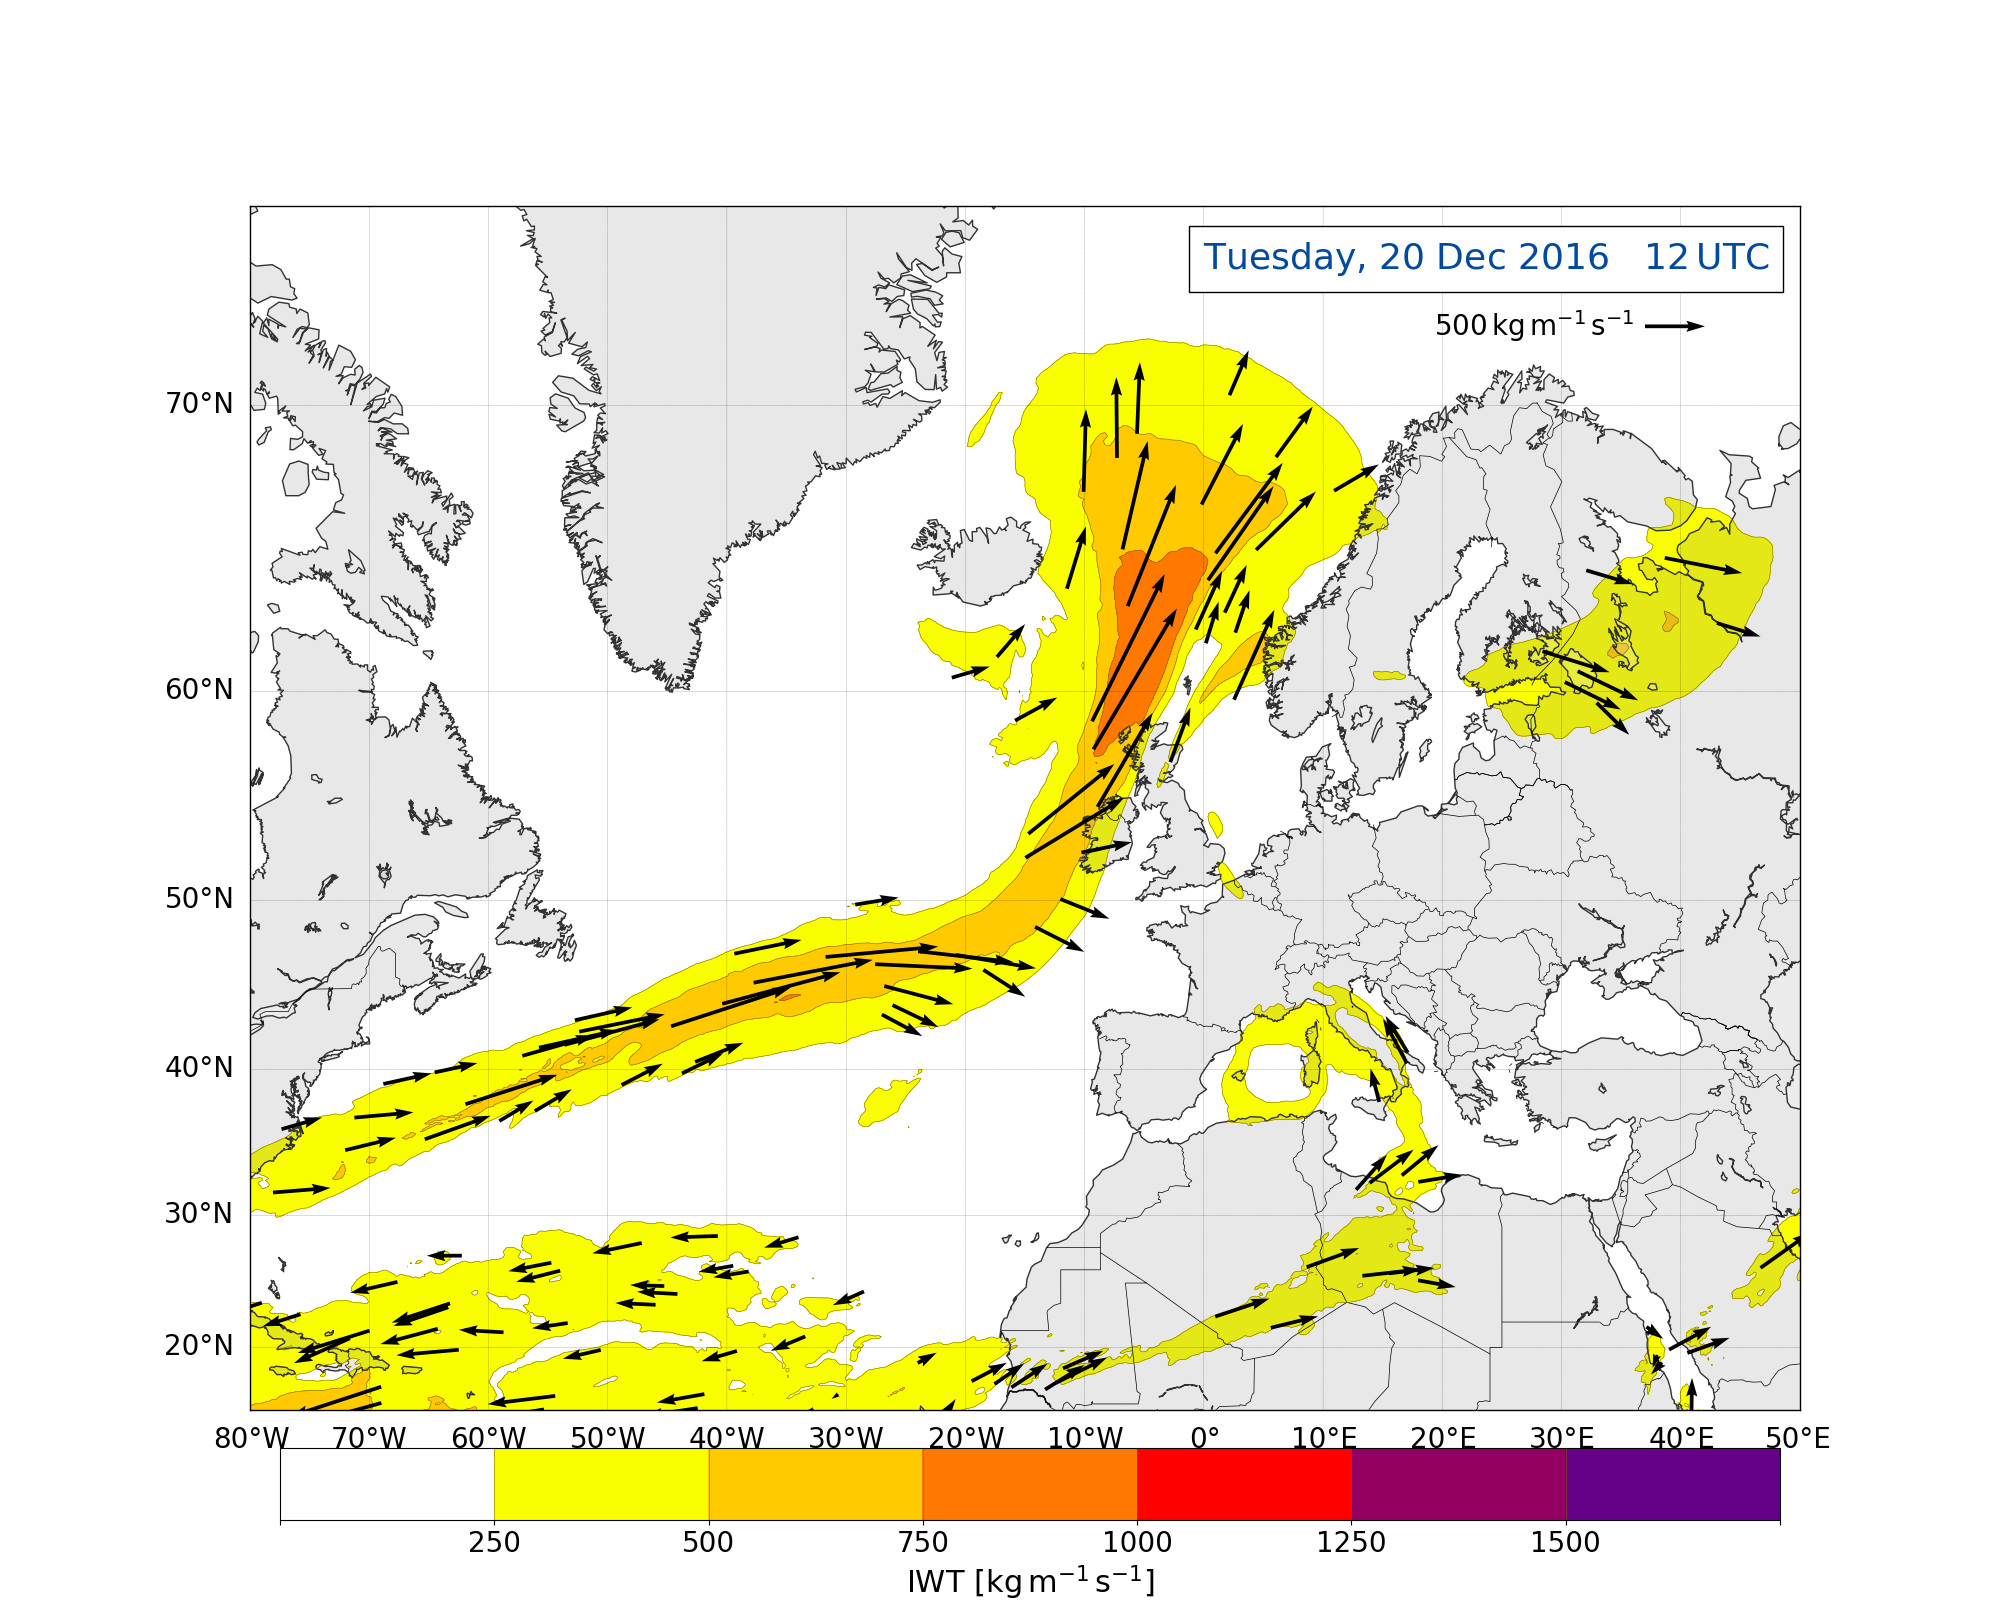
\includegraphics[trim={4.2cm 3.9cm 4.3cm 5.1cm},clip,
		width=\textwidth]{./fig_Atm_Riv/20161220_12}
		\caption{}\label{fig:AR20}
	\end{subfigure}
	%%%%%% 21/12
	\begin{subfigure}[b]{0.49\textwidth}
		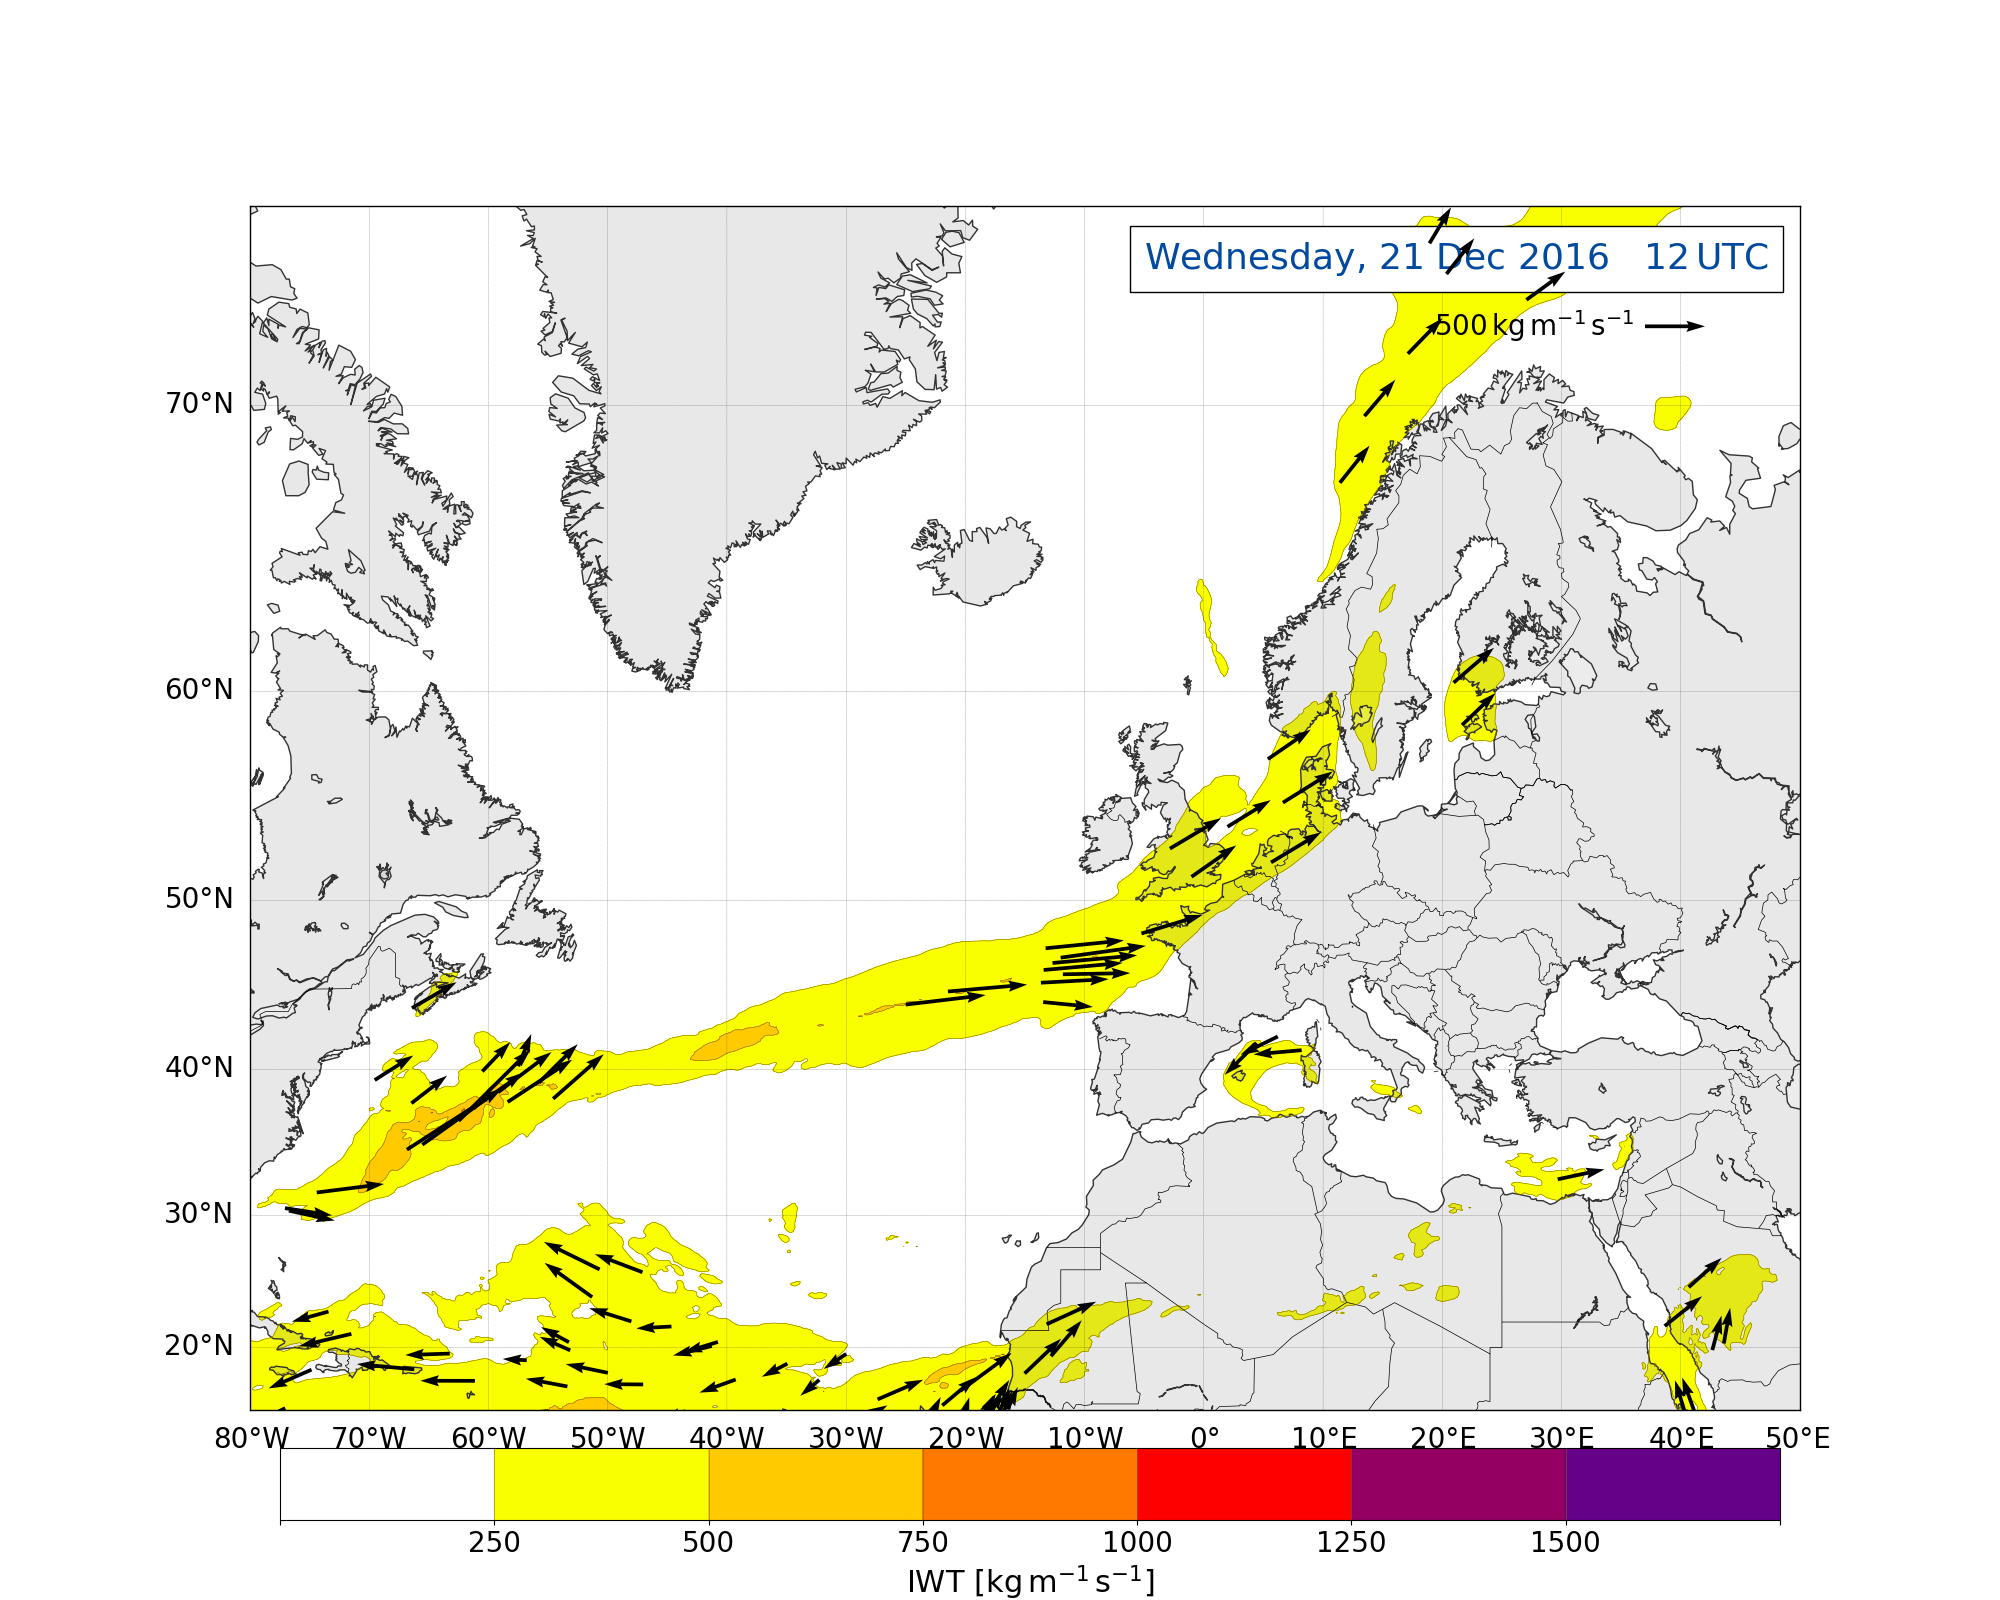
\includegraphics[trim={4.2cm 3.9cm 4.3cm 5.1cm},clip,
		width=\textwidth]{./fig_Atm_Riv/20161221_12}
		\caption{}\label{fig:AR21}
	\end{subfigure}
	%%%%%% label
	\begin{subfigure}[b]{\textwidth}
		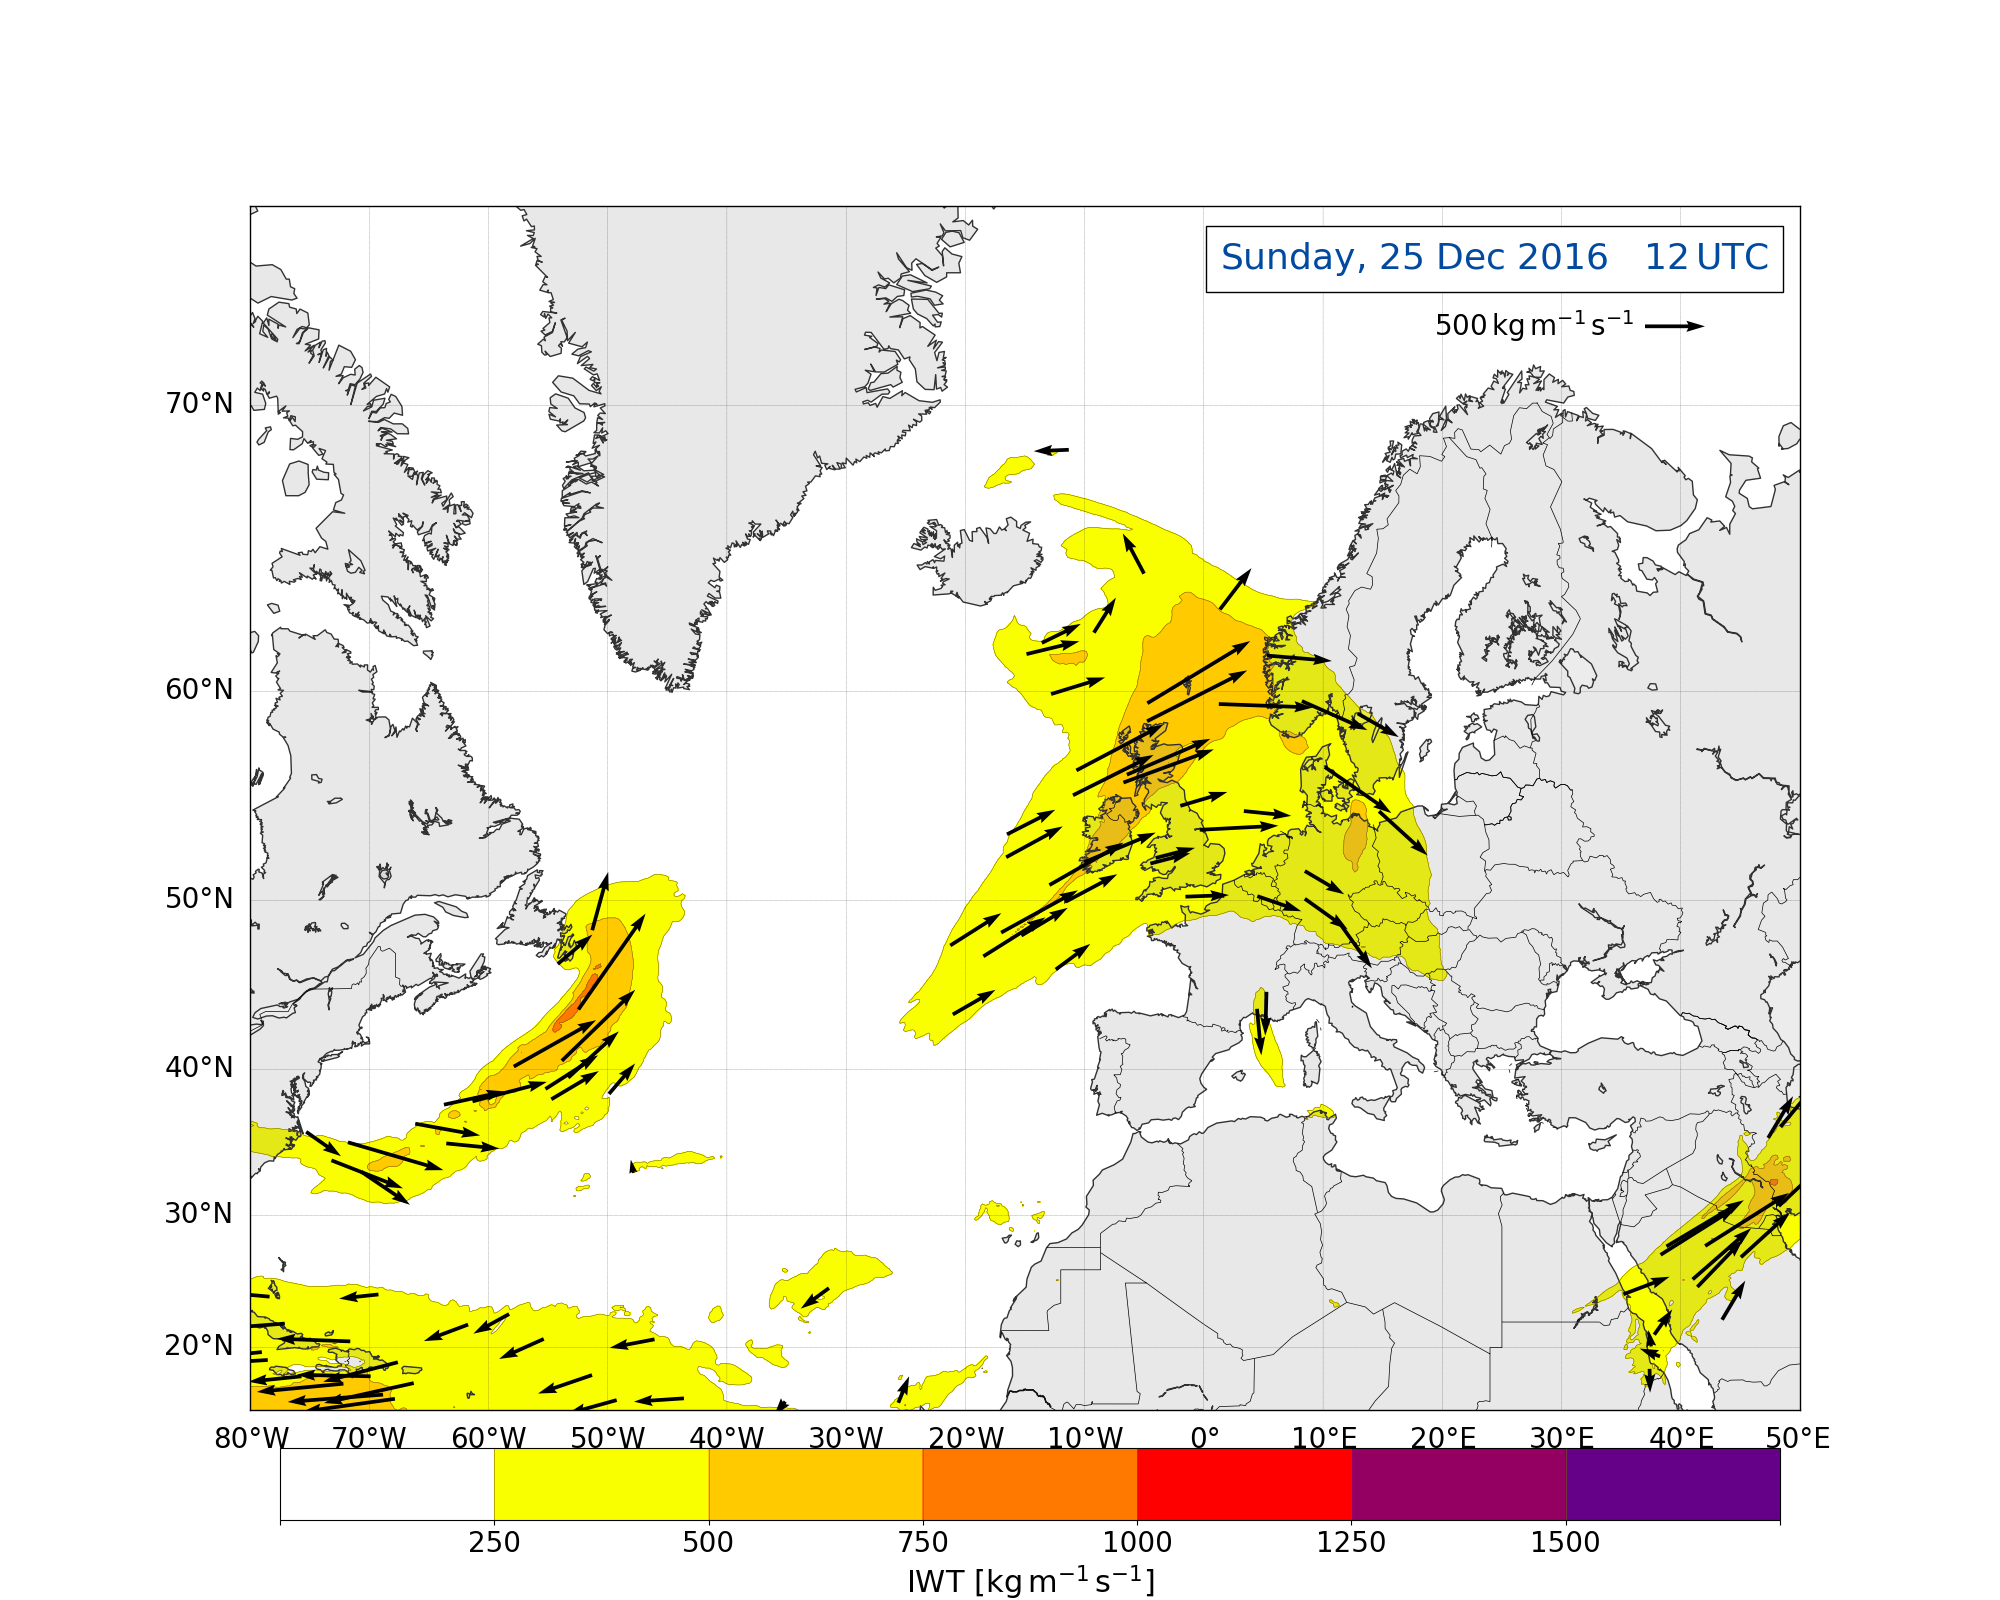
\includegraphics[trim={4.2cm 0cm 4.3cm 36.8cm},clip,
		width=\textwidth]{./fig_Atm_Riv/20161225_12}
	\end{subfigure}
\end{figure}
%
\begin{figure}\ContinuedFloat
	\centering
	%%%%%% 22/12
	\begin{subfigure}[b]{0.49\textwidth}
		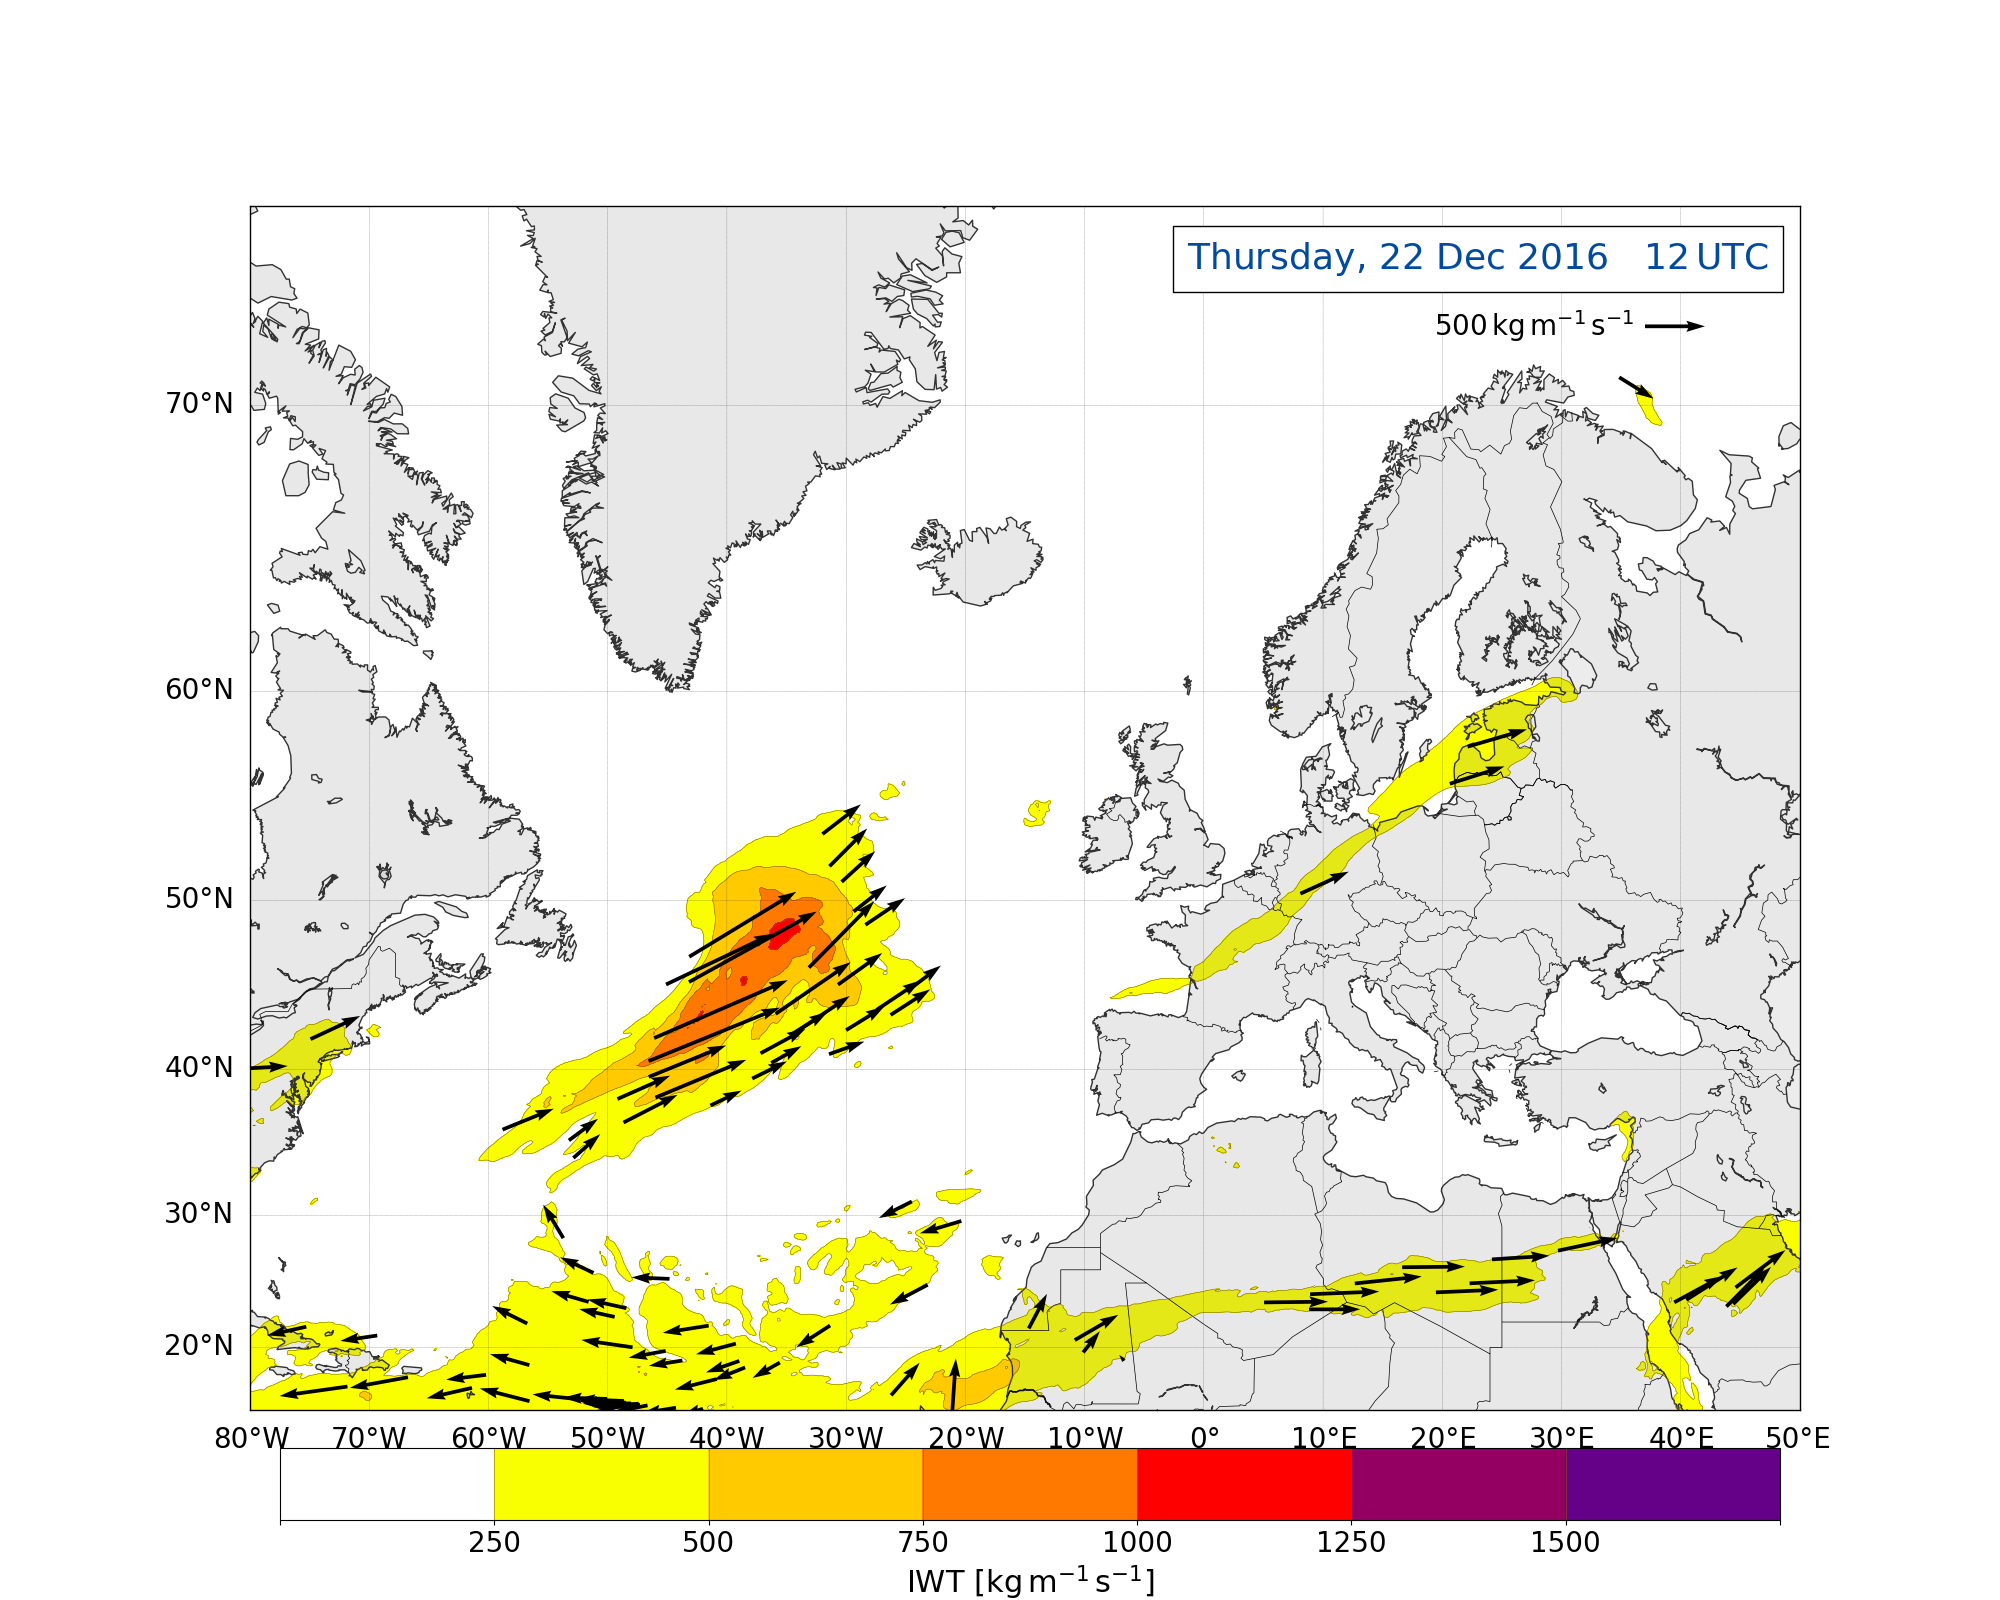
\includegraphics[trim={4.2cm 3.9cm 4.3cm 5.1cm},clip,
		width=\textwidth]{./fig_Atm_Riv/20161222_12}
		\caption{}\label{fig:AR22}
		%\label{fig:sfc2100}
	\end{subfigure}
	%%%%%% 23/12
	\begin{subfigure}[b]{0.49\textwidth}
		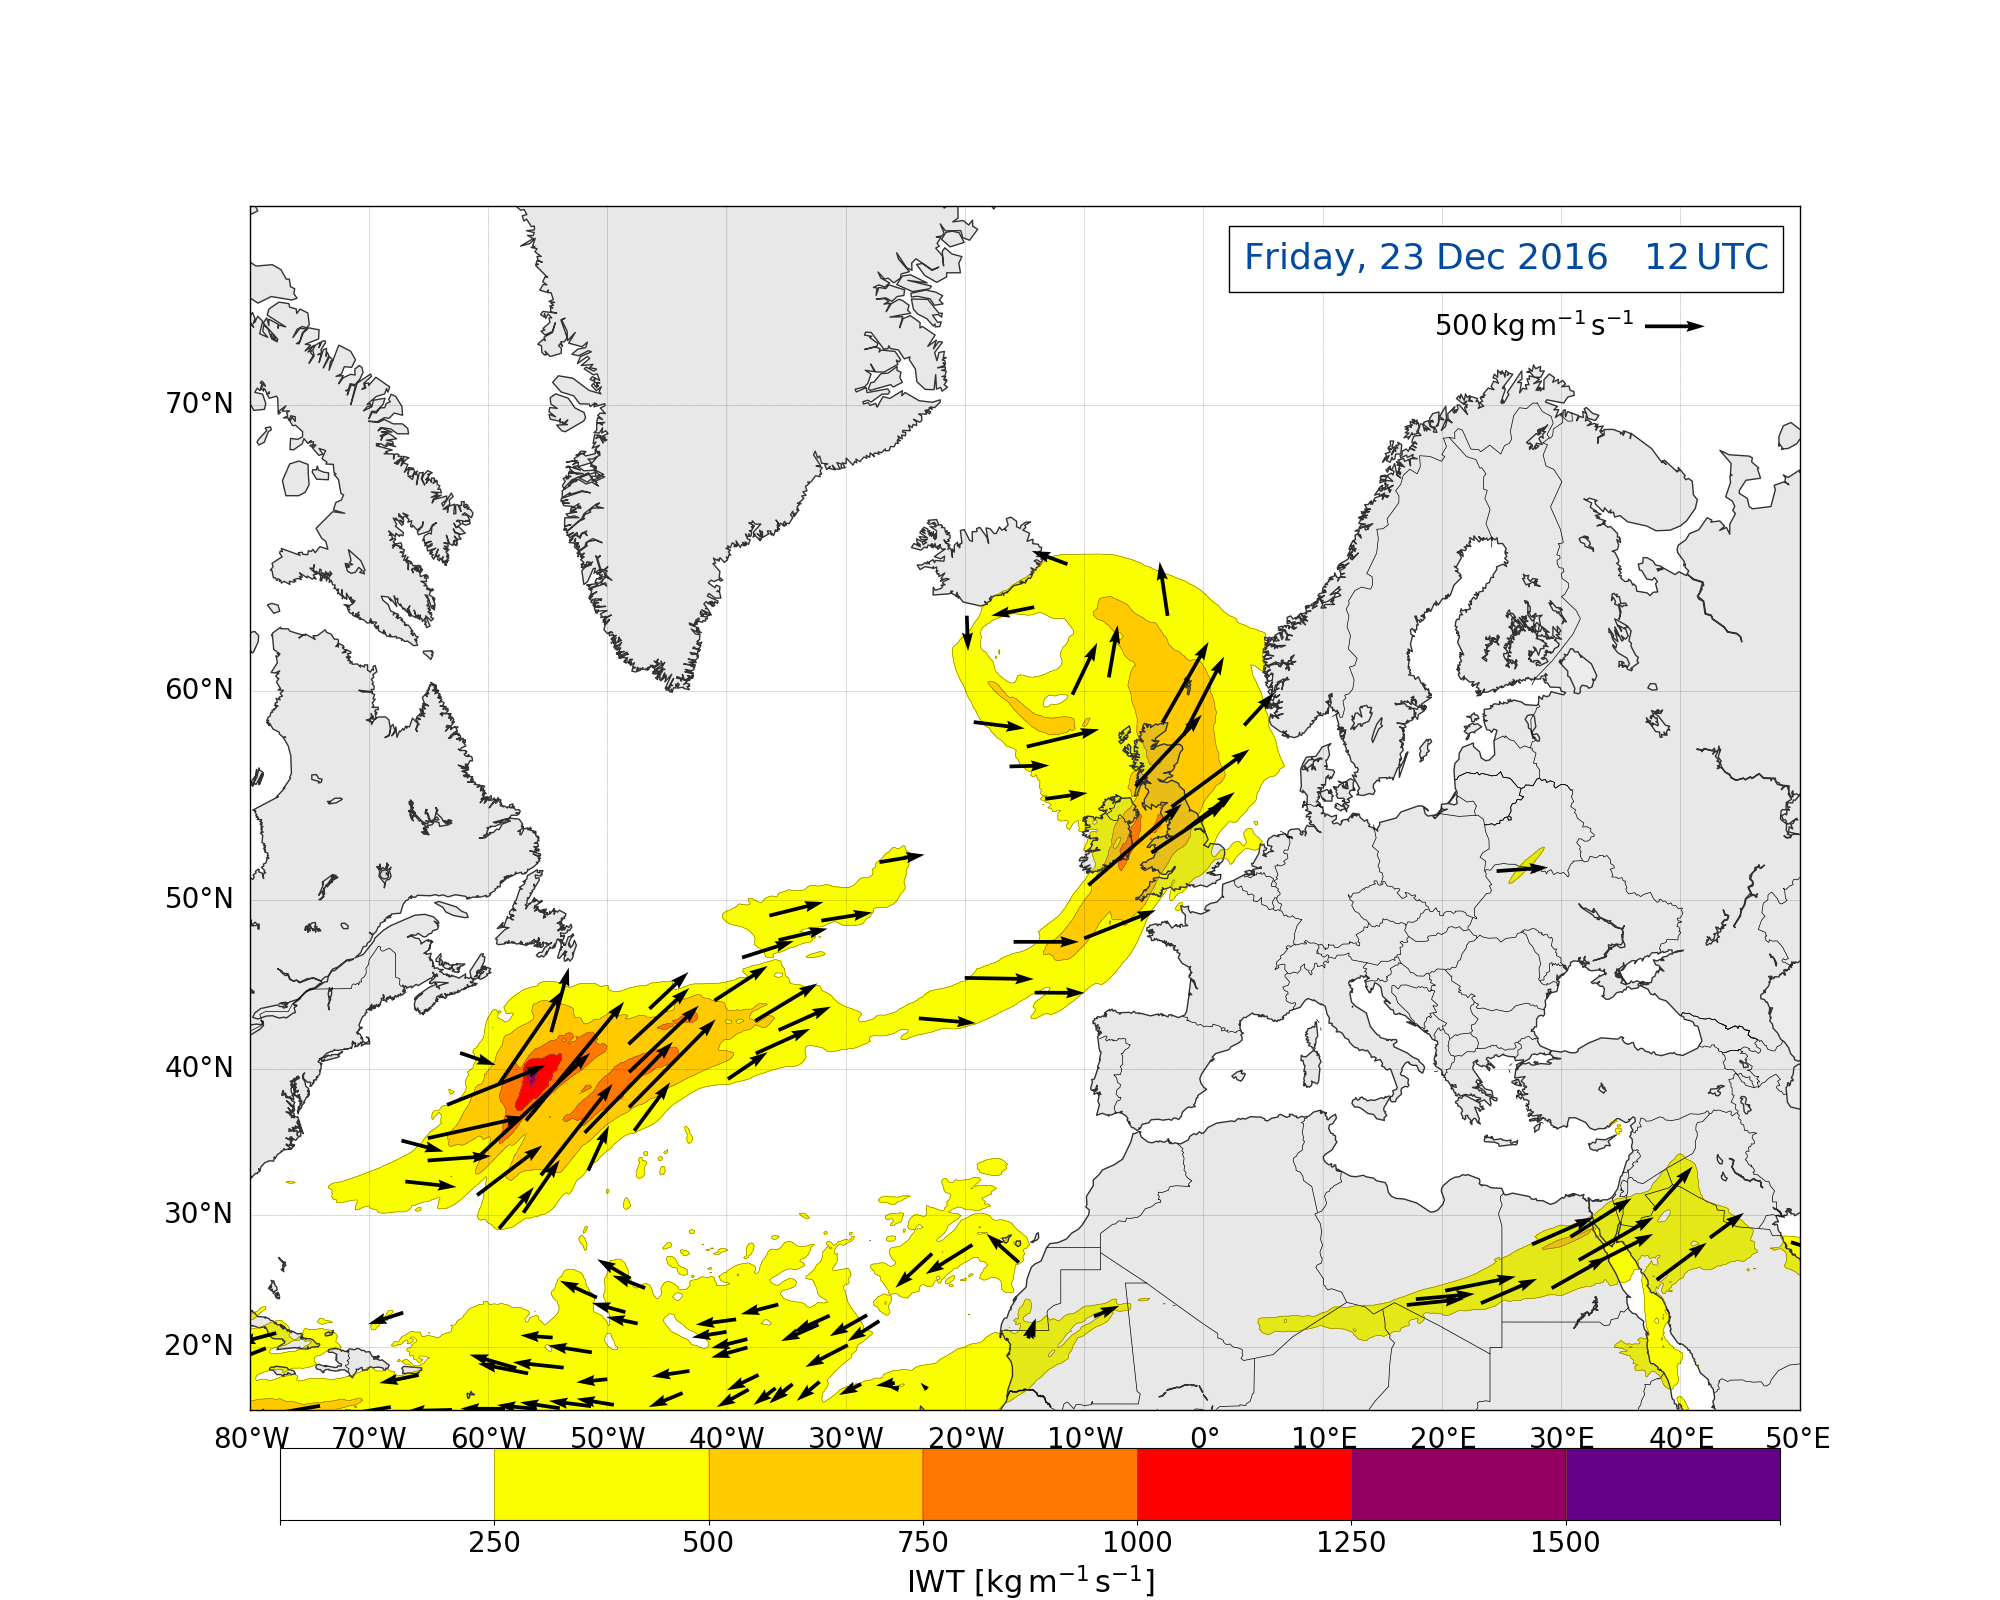
\includegraphics[trim={4.2cm 3.9cm 4.3cm 5.1cm},clip,
		width=\textwidth]{./fig_Atm_Riv/20161223_12}
		\caption{}\label{fig:AR23}
	\end{subfigure}
	%%%%%% 24/12
	\begin{subfigure}[b]{0.49\textwidth}
		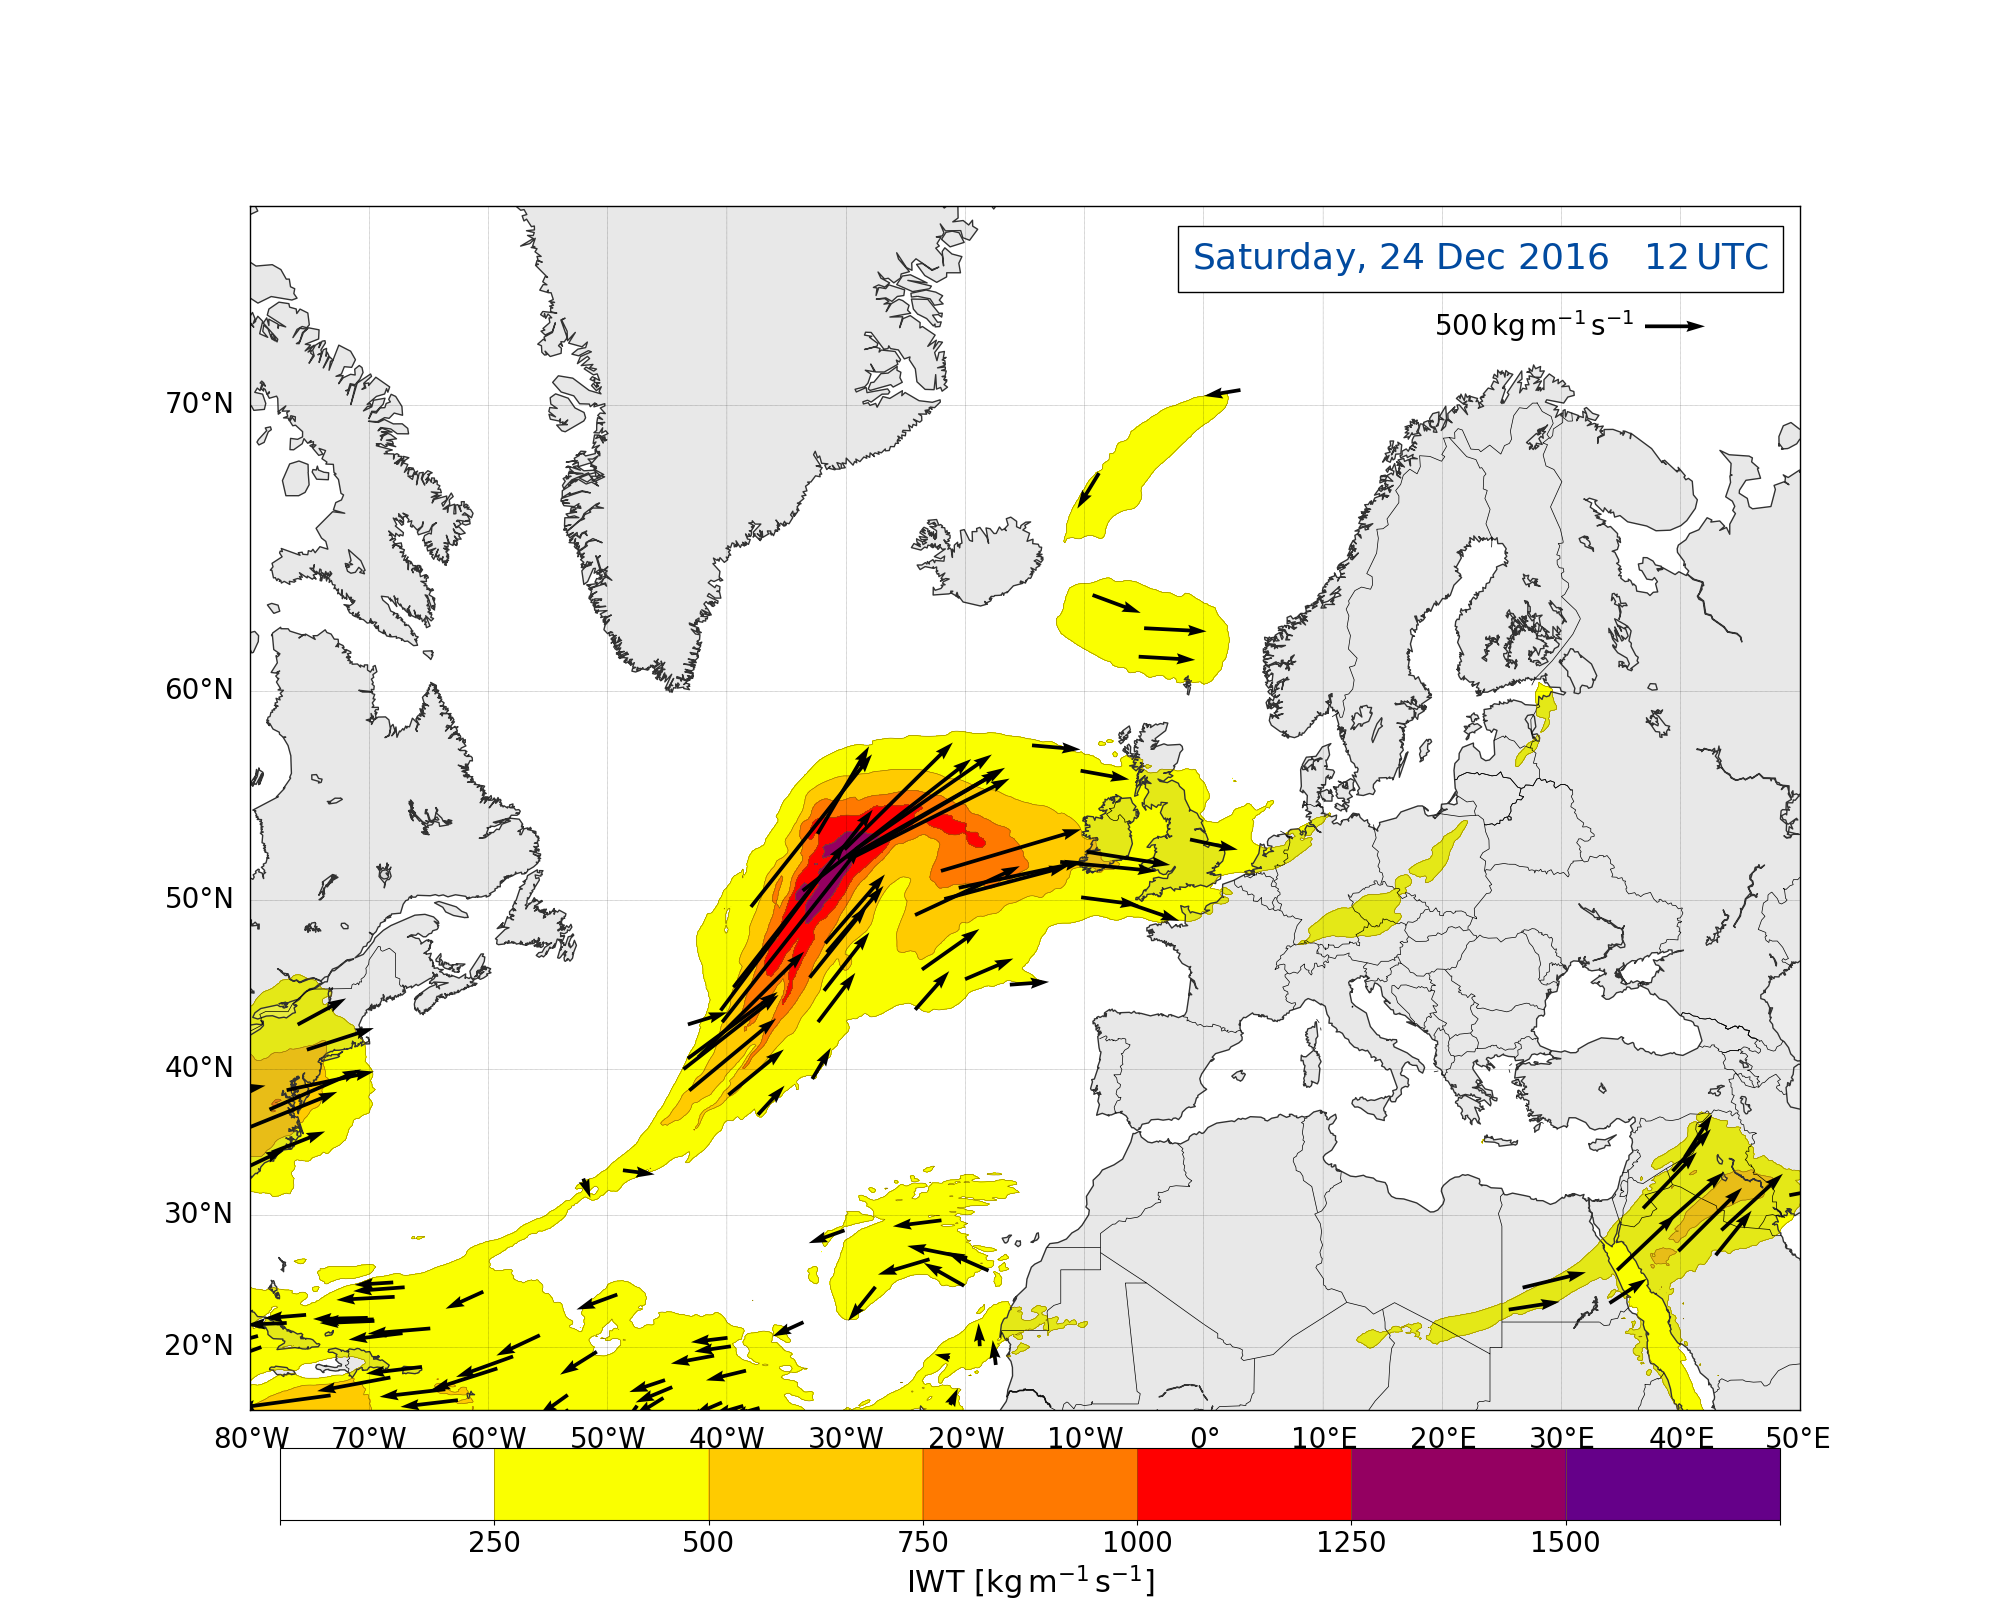
\includegraphics[trim={4.2cm 3.9cm 4.3cm 5.1cm},clip,
		width=\textwidth]{./fig_Atm_Riv/20161224_12}
		\caption{}\label{fig:AR24}
	\end{subfigure}
	%%%%%% 25/12
	\begin{subfigure}[b]{0.49\textwidth}
		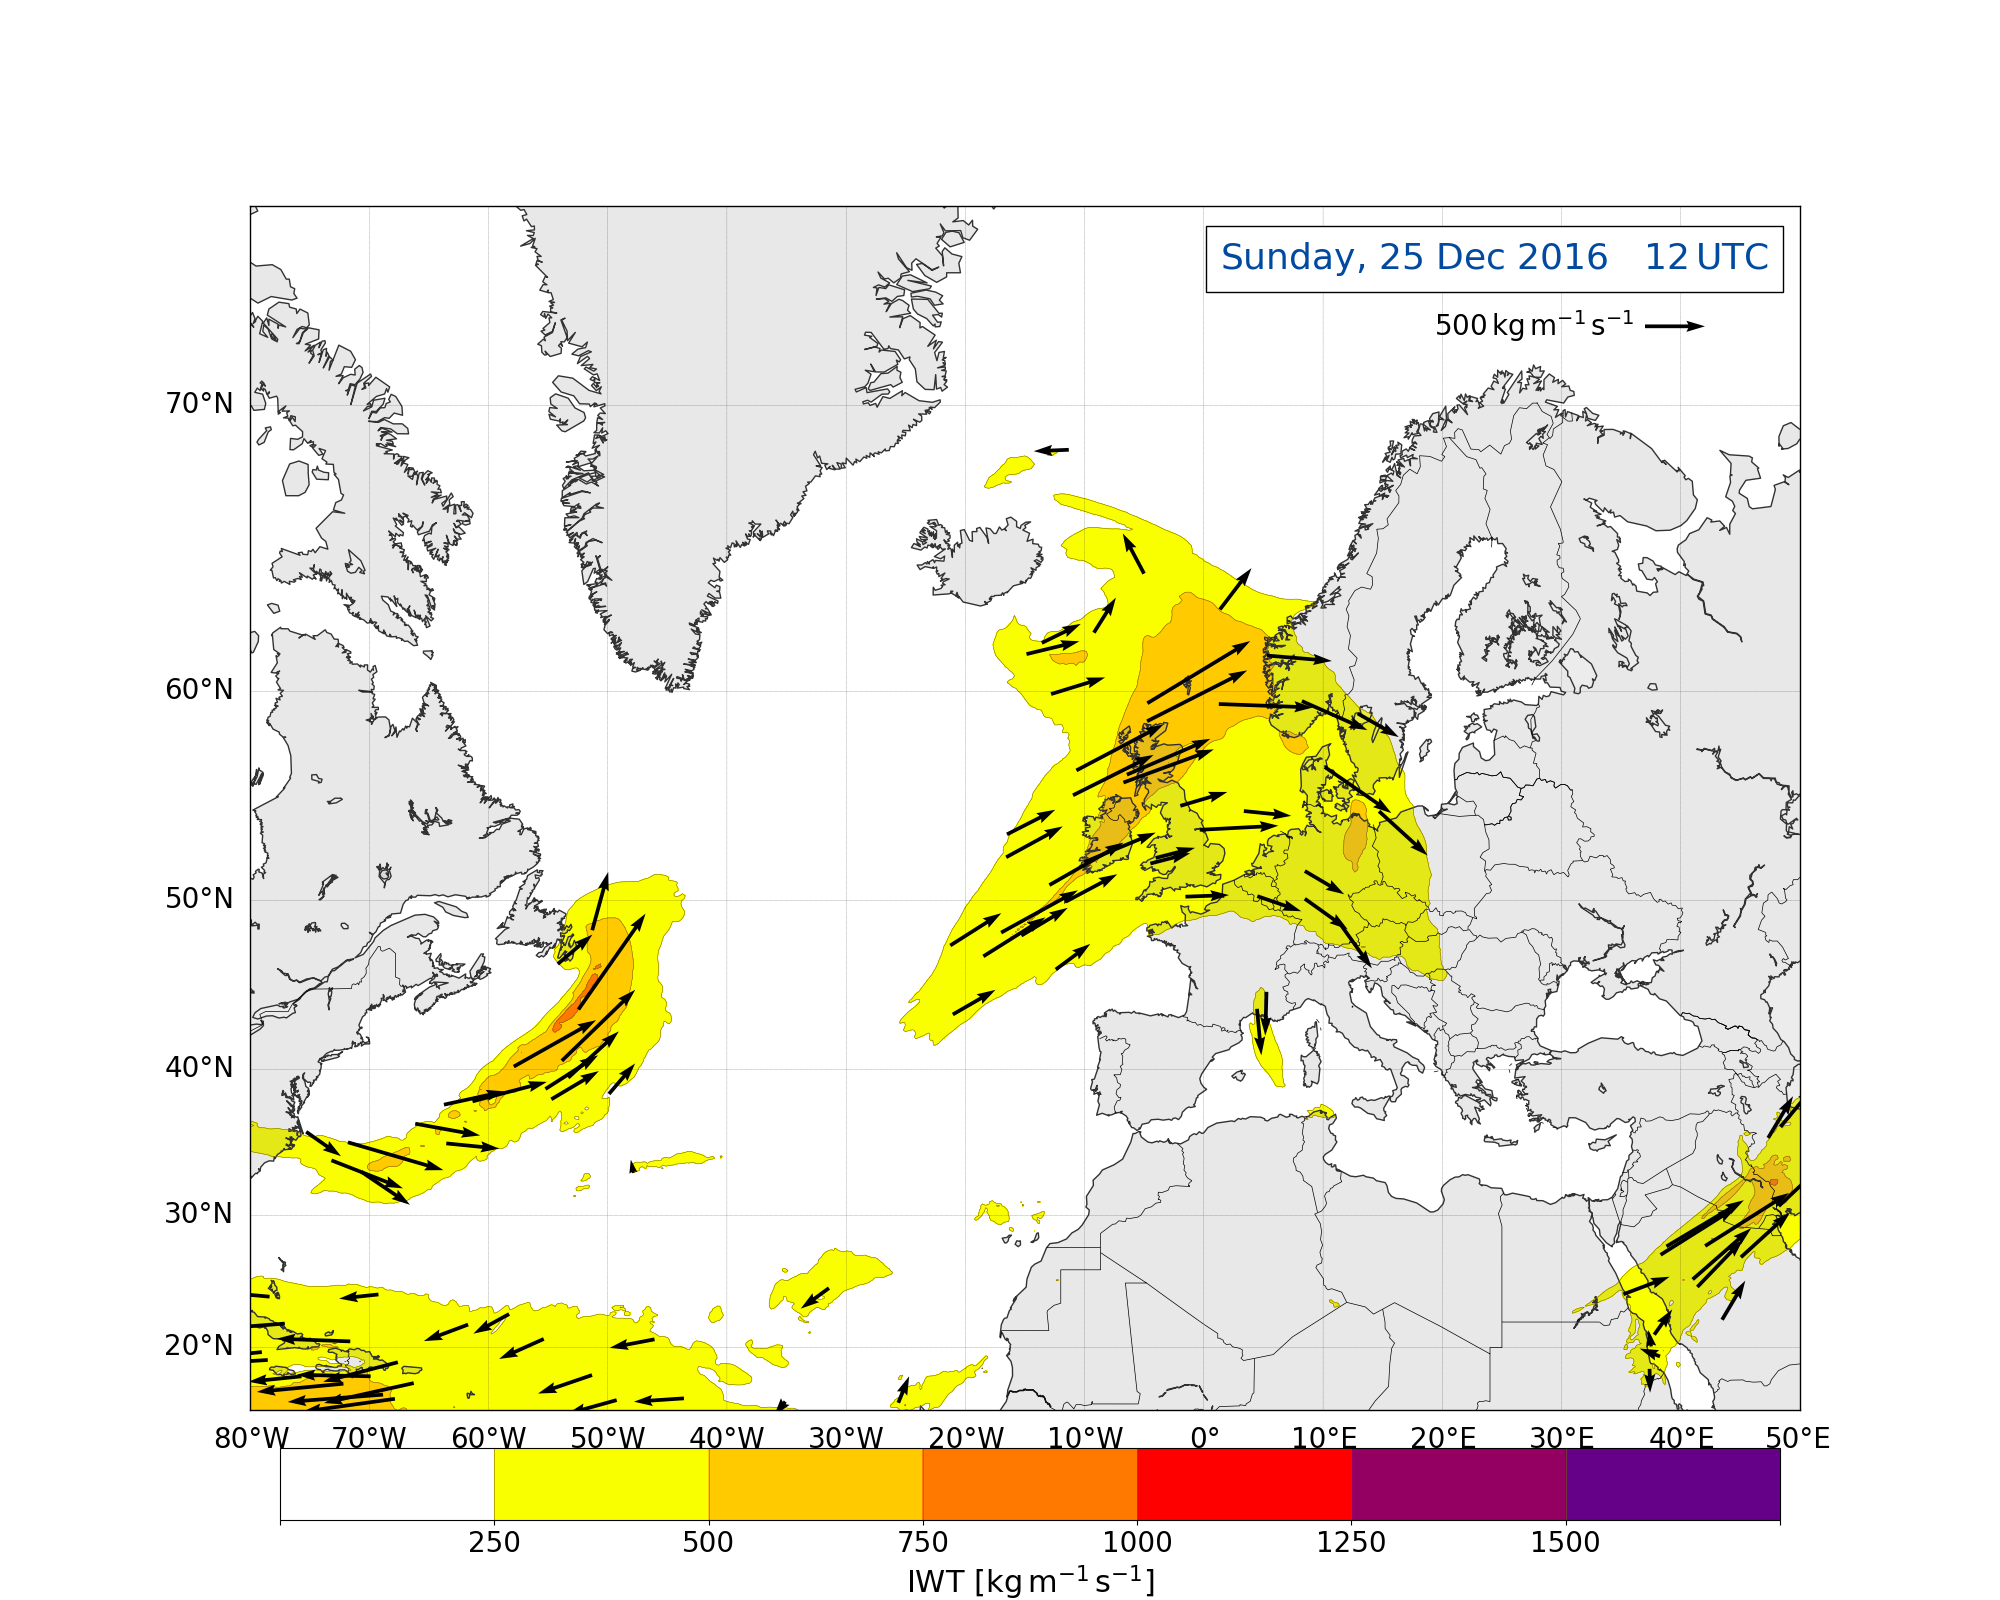
\includegraphics[trim={4.2cm 3.9cm 4.3cm 5.1cm},clip,
		width=\textwidth]{./fig_Atm_Riv/20161225_12}
		\caption{}\label{fig:AR25}
	\end{subfigure}
	%	\centering
	%%%%%% 26/12
	\begin{subfigure}[b]{0.49\textwidth}
		\includegraphics[trim={4.2cm 3.9cm 4.3cm 5.1cm},clip,
		width=\textwidth]{./fig_Atm_Riv/20161226_12}
		\caption{}\label{fig:AR26}
	\end{subfigure}
	%%%%%% 27/12
	\begin{subfigure}[b]{0.49\textwidth}
		\includegraphics[trim={4.2cm 3.9cm 4.3cm 5.1cm},clip,
		width=\textwidth]{./fig_Atm_Riv/20161227_12}
		\caption{}\label{fig:AR27}
	\end{subfigure}
	%%%%%% label
	\begin{subfigure}[b]{\textwidth}
		\includegraphics[trim={4.2cm 0cm 4.3cm 36.8cm},clip,
		width=\textwidth]{./fig_Atm_Riv/20161225_12}
	\end{subfigure}
	\caption{Atmospheric river analysis map, data from ECMWF. During \SIrange{20}{27}{\dec}. IVT, shaded according to the colour bar [\SI{}{\IVT}]. Vectors, indicating the direction and magnitude of the IVT. }\label{fig:AtmRiv}
\end{figure}
%%%%%%%%%%%%%%%%%%%%%%%%%%%%%%%%%%%%%%%%%%%%%%%%%%%%%%%%%%%%%%%%%%%%%%%%%
%%%%%%%%%%%%%%%%%%%%%%%%%%%%%%%%%%%%%%%%%%%%%%%%%%%%%%%%%%%%%%%%%%%%%%%%%

%%%%%%%%% WEATHERMAST OBSV %%%%%%%%%%%%%%
% !TeX spellcheck = en_GB
\section{Observations at the weather mast}
\label{sec:loc_obs}
The large scale synoptic analysis will be related to the local weather  observations at Haukeliseter. 
\\
\SI{60}{\minute} accumulation is presented as bars in \Cref{fig:TPU} and will show the continuous precipitation at Haukeliseter during the extreme event. The possible change of precipitation will be investigated with the temperature. Snow fall is likely for temperatures up to \SI{2}{\celsius}. The intensity of the storm can be classified by the hourly averaged wind speed and direction as wind barbs in \SI{}{\mPs}.
To understand which damage a storm can have, \cite{faeraas_urd_2016} released a table to associate wind strength with damage (see \Cref{tab:wind}).
%%% Damage related to wind speed %%%%%%%%%%%%%%%%%%%%%%%%%%%%%%%%%%%%%
% !TeX spellcheck = en_GB
\begin{table}[h!]
	\begin{center}
		\caption{Damage related to wind speed, from \cite{faeraas_urd_2016}. }\label{tab:wind}
		\begin{tabular}{l|c|l}
			\hline \hline
			slight storm& \SI{20.8}{\mPs} -- \SI{24.4}{\mPs}&  Large trees sway and hiver. \\
			&  &  Roofs can blow down. \\ \hline
			full storm & \SI{24.5}{\mPs} -- \SI{28.4}{\mPs}& Trees are pulled up with clutter. \\
			&  & Big damages to houses.\\ \hline
			strong storm & \SI{28.5}{\mPs} -- \SI{32.6}{\mPs}& Extensive damage.\\
			&  & \\ \hline
			hurricane & \textgreater \SI{32.6}{\mPs}& Unusually large destruction.\\
			\hline \hline
		\end{tabular}
	\end{center}
\end{table}
%%%%%%%%%%%%%%%%%%%%%%%%%%%%%%%%%%%%%%%%%%%%%%%%%%%%%%%%%%%%%%%%%%%%%%%%%%
%%% local observations @ Haukeliseter %%%%%%%%%%%%%%%%%%%%%%%%%%%%%%%%%%%%%
% !TeX spellcheck = en_GB
\begin{figure}[h!]
	\centering
	%%%%%% 20/12
	\begin{subfigure}[b]{0.49\textwidth}
		\includegraphics[trim={4.9cm 1.cm 1.5cm 1cm},clip,
		width=\textwidth]{./fig_weathermast/T_P_U_20161220}
		\caption{}\label{fig:TPU20}
	\end{subfigure}
	\hfill
	%%%%%% 21/12
	\begin{subfigure}[b]{0.49\textwidth}
		\includegraphics[trim={4.9cm 1.cm 1.5cm 1cm},clip,
		width=\textwidth]{./fig_weathermast/T_P_U_20161221}
		\caption{}\label{fig:TPU21}
	\end{subfigure}
% \end{figure}
% \begin{figure}\ContinuedFloat
	\centering
	%%%%%% 22/12
	\begin{subfigure}[b]{0.49\textwidth}
		\includegraphics[trim={4.9cm 1.cm 1.5cm 1cm},clip,
		width=\textwidth]{./fig_weathermast/T_P_U_20161222}
		\caption{}\label{fig:TPU22}
	\end{subfigure}
	\hfill
	%%%%%% 23/12
	\begin{subfigure}[b]{0.49\textwidth}
		\includegraphics[trim={4.9cm 1.cm 1.5cm 1cm},clip,
		width=\textwidth]{./fig_weathermast/T_P_U_20161223}
		\caption{}\label{fig:TPU23}
	\end{subfigure}
	%\end{figure}
	%\begin{figure}[h]\ContinuedFloat
	%%%%%% 24/12
	\begin{subfigure}[b]{0.49\textwidth}
		\includegraphics[trim={4.9cm 1.cm 1.5cm 1cm},clip,
		width=\textwidth]{./fig_weathermast/T_P_U_20161224}
		\caption{}\label{fig:TPU24}
	\end{subfigure}
	\hfill
	%%%%%% 25/12
	\begin{subfigure}[b]{0.49\textwidth}
		\includegraphics[trim={4.9cm 1.cm 1.5cm 1cm},clip,
		width=\textwidth]{./fig_weathermast/T_P_U_20161225}
		\caption{}\label{fig:TPU25}
	\end{subfigure}
	%%%%%% 26/12
	\begin{subfigure}[b]{0.49\textwidth}
		\includegraphics[trim={4.9cm 1.cm 1.5cm 1cm},clip,
		width=\textwidth]{./fig_weathermast/T_P_U_20161226}
		\caption{}\label{fig:TPU26}
	\end{subfigure}
	\hfill
	%%%%%% 27/12
	\begin{subfigure}[b]{0.49\textwidth}
		\includegraphics[trim={4.9cm 1.cm 1.5cm 1cm},clip,
		width=\textwidth]{./fig_weathermast/T_P_U_20161227}
		\caption{}\label{fig:TPU27}
	\end{subfigure}
	\caption{Observation from the weather mast at Haukeliseter during \SIrange{20}{27}{\dec}. \SI{60}{\minute} total accumulation [\SI{}{\mm}] in light blue as bar, temperature (red, [\SI{}{\celsius}]), and wind as barbs [\SI{}{\mPs}]. Gray dashed line indicates the freezing temperature and the green dashed line the 30-year climate mean temperature at \SI{-6}{\celsius}. Hourly processed data taken from \cite{eklima_norwegian_2016}.} \label{fig:TPU}
\end{figure}
%%%%%%%%%%%%%%%%%%%%%%%%%%%%%%%%%%%%%%%%%%%%%%%%%%%%%%%%%%%%%%%%%%%%%%%%%%
%%%%%%%%%%%%%%%%%%%%%%%%%%%%%%%%%%%%%%%%%%%%%%%%%%%%%%%%%%%%%%%%%%%%%%%%%%

%%%%%%%%%% LARGE SCALE CIRCULATION %%%%%%%%%%%%%%
% !TeX spellcheck = en_GB
\section{Large scale circulation} \label{sec:largeScale}
\textcolor{red}{Everything has to get into relation with the Radiosondes, \Cref{fig:sounding}. How to do that? Any suggestions? They took me some time to make, so I want to include them!}
%%% 21/12
% 21/00
% Westerly flow, perfect for orographic lifting
% → lots of moisture (check for correct values)
% Cold air goes right over Norway 
% → probably snow
% 21/18
% Low forming right at the main baroclinic zone (~45°N, south of Greenland)
% Formation @ the right entrance region of the jet, which helps for lifting
\subsection*{\SI{21}{\dec}}
The dynamic tropopause map in \Cref{fig:DT21} shows that Norway is influenced by a change of elevated tropopause to a suppressed tropopause during \SIrange{20}{21}{\dec}. Hence the potential vorticity changed from positive to negative at the tropopause and cold air stretches right over Norway.
A good amount of moisture is transported from the low latitudes to high latitudes, influencing Norways' west coast. This can be seen in the surface maps (\Cref{fig:GP21}) as well as in the atmospheric river maps (\Cref{fig:AR21}). The westerly flow in \Cref{fig:GP21} is conducive to orographic lifting. The precipitation was probably snow when having a look at the moisture content and the cold air. The change from warm air to cold air can also be observed in the time series of temperature in \Cref{fig:TPU21}. And the westerly flow, combined with a good amount of vapour transport from the tropics led to orographic lifting and precipitation at the Haukeliseter site. 
At around \ang{60}{\,W} a formation of a cyclone at the baroclinic zone can be implied.  

\subsection*{\SI{22}{\dec}}
%%% 22/12
% 22/12
% @ DT, phasing of the vorticity
% → low center is in perfect condition for synoptic scale lifting
\noindent Twenty-four hours later the analysis shows from \SI{22}{\dec} phasing between the surface relative vorticity and the baroclinic zone at \ang{50}{\,N} in the DT. The centre of the surface low is directly located below the temperature gradient at the \SI{2}{PVU} surface, hence this is good for synoptic lifting. Furthermore, the strongest baroclinicity is observed on the south west side of the surface low.
The synoptic map of the geopotential thickness and the surface pressure show the beginning of the frontal boundaries in \Cref{fig:GP22}. 
At the same time shows the AR map, \Cref{fig:AR22}, large values just at the baroclinic zone, where the low pressure is beginning to form. \textcolor{red}{Help?! Does that lead to even more lifting in this area? Or does it just mean that the cyclone gets a good amount of moisture?!}.
Norway is located in a cold area. The continues precipitation observed at Haukeliseter (\Cref{fig:TPU22}) is associated with the westerly flow which is conducive to orographic lifting, and therefore moisture release.  

\subsection*{\SI{23}{\dec}}
%%% 23/12
% 23/06
% Still conducive westerly flow → orographic lifting
% Norway in cold area
% Jet not very strong
% Probably frozen precipitation
% Baroclinicity strongest South West of low center
% Low has well formed frontal boundaries (low level vorticity, → lifting at the cold frontal boundary?)
% 23/12
% Westerlies change
% That is because of the ridging @ DT
% → pushes away the cold air
% First frontal boundary (warm front/Occluded front?) goes through
% 23/18
% Frontal boundary went through, warms up → probably mixed phase/liquid precip.
% Lifting associates with the warm front
% Some forcing due to low level flow / weak warm front
% Southern Norway is briefly into warm air mass, before the cold front comes along
\noindent The begin of the ridging on the \SI{22}{\dec} is more pronounced \SI{24}{\hour} later. The warmer air pushes away the cold air, which covered Norway.
The low pressure system moved north-east, and lies south of Iceland. The occluded front of this system passes through Haukeliseter, which is why a temperature 'jump' observed at \SI{14}{\UTC}. After this, Southern Norway is influenced by the warm sector, monitored as a temperature increase. 
The AR, as well as the total column water vapour amount in \Cref{fig:AR23} and \Cref{fig:GP23}, respectively show the amount of moisture, transported from low latitudes.
\\
At the same time forms a second cyclone at the baroclinic zone at \ang{40}{\,N}. The atmospheric river map (\Cref{fig:AR23}) indicates a large amount of moisture at this latitude. Again, moist, warm air is conducive to intensify the surface cyclone. In addition, shows the DT map a phasing between the low level vorticity and the upper level baroclinic zone. 

\subsection*{\SI{24}{\dec}}
%%% 24/12
% 24/00
% Norway goes right back into colder air @ DT, @ sfc (thickness lines)
% @ DT lifting associated with the low-level vorticity 
% 24/12
% Cold frontal boundary pushes through
% Norway is back into colder air → reduction in temp.
% Again westerly flow → good for orographic lifting
\noindent After the passage of the cold front over Norway, Scandinavia is within colder air (compare \Cref{fig:DT24} and \Cref{fig:GP24} for \SI{24}{\dec}). Over the Atlantic warmer air starts to push the colder air northward. \textcolor{red}{something something with the low level vorticity and lifting; lifting at the right entrance region of the jet streak, and very high IVT}.
\\
At Haukeliseter negative temperature up to \SI{-4}{\celsius} is observed, compare \Cref{fig:TPU24}. The westerly flow is again conducive for orographic lifting and associated precipitation.

\subsection*{\SI{25}{\dec}}
%%% 25/12
% 25/00
% @ DT ridging coming in
% @ sfc, low with frontal boundaries
% Jet exit region is directly over Norway → Haukeliseter on right exit region? → sinking?
% Some orographic lifting
% 25/12
% Warm front comes through
% → low-level vorticity → orographic lifting
% 25/18
% Ridging bring more warm air to Norway (should be moist too → check total water vapor)
% Norway in warm sector
% Conducive westerly flow → orographic lifting
\noindent Twenty-four hours later the ridge is more pronounced and covers large parts of Norway. The surface low south-east of Iceland has build its frontal boundaries, which can be seen in the low-level vorticity of \Cref{fig:DT25}. The warm front lies west of Haukeliseter and starts to be observed at the measurement site (compare \Cref{fig:TPU25} for \SI{25}{\dec}). \Cref{fig:AR25} indicating the integrated vapour transport shows that a lot of moisture is transported from the Atlantic, towards Great Britain and south-western Norway. Together with the lifting at the surface boundary a sufficient amount of precipitation is observed. 
\\
Since the ridging brings more moist (\Cref{fig:AR25}), warm air (\Cref{fig:DT25}) and Norway lies in a warm sector (\Cref{fig:GP25}) the assumption will be made, that the precipitation changed from solid to liquid. 

\subsection*{\SI{26}{\dec}}
%%% 26/12
% 26/06
% Cold front went through
% Norway lies in cold area (@ sfc: blue thickness lines, @ DT: cold anomaly)
% 26/18
% North westerly flow at west coast of Norway
% Conducive for orographic lifting, @ DT: strong low-level vorticity gradient
\noindent Within the next twenty-four hours the cold front passed through (temperature change in \Cref{fig:TPU26} for \SIrange{25}{26}{\dec}). Norway is covered in cold air (\Cref{fig:DT26}). The surface low-level indicates the occlusion of the cyclone and therefore a weakening. The wind is still from the west which is helpful for orographic lifting. The moisture content is still present but much weaker and smaller in extend. Since Norway is covered in cold air, the temperature is below zero and the precipitation had to be solid. 

\subsection*{\SI{27}{\dec}}
%%% 27/12
\noindent
The images of \SI{27}{\dec} show that the storm passed and disappeared. Southern Norway lies in cold air (\Cref{fig:DT27}), but on the right exit region of the jet ($\rightarrow$ sinking motion of cold air), compare \ref{fig:GP27}. A small amount of moisture is present (\Cref{fig:AR27}). Because of the wind change from west to north-west follows that orographic lifting is not present and the precipitation amount decreases at the end of the storm. 





